\documentclass[b5paper,11pt,twoside]{scrbook} %176x250mm
\usepackage[utf8]{inputenc}  
\usepackage[T1]{fontenc}      % Unterstützung für Europäische-Zeichen-Ausgabe
%\usepackage{ae}               % verbesserte Unterstützung für Umlaute
\usepackage[ngerman]{babel}% deutsche Übersetzungen und Wortumbrüche
\usepackage[autostyle=true,german=quotes]{csquotes}
\usepackage[scaled=.90]{helvet}  % schönere Schriftart: Helvetica
\usepackage{graphicx}              % Unterstützung für Graphiken
\usepackage[                
   pdftex,                  % Ausgabe-Medium: PDF
   colorlinks=true,         % farbige Links in der Bildschirm-Version?
   linkcolor=blue,          % Farbe für Querverweise
   citecolor=black,         % Farbe für Zitierungen
   urlcolor=blue,           % Farbe für Links
   bookmarks=true
   ]{hyperref}             % Paket für Links im PDF
\usepackage[backend=biber, %% Hilfsprogramm "biber" (statt "biblatex" oder "bibtex")
style=verbose-inote, %% Zitierstil (siehe Dokumentation)
natbib=true, %% Bereitstellen von natbib-kompatiblen Zitierkommandos
hyperref=true, %% hyperref-Paket verwenden, um Links zu erstellen
]{biblatex}
\addbibresource{literatur.bib}
\usepackage{listings,makeidx} \makeindex
\usepackage{array,longtable} 
\usepackage{mdframed}
\mdfsetup{skipabove=\topskip,skipbelow=\topskip}
%\newcounter{tip}[section]
\newenvironment{tip}[1][]{%
%\stepcounter{tip}%
\ifstrempty{#1}%
{\mdfsetup{%
frametitle={%
\tikz[baseline=(current bounding box.east),outer sep=1pt]
\node[anchor=east,rectangle,fill=pumablue!40]
{\strut Hinweis};}}
}%
{\mdfsetup{%
frametitle={%
\tikz[baseline=(current bounding box.east),outer sep=1pt]
\node[anchor=east,rectangle,fill=pumablue!40]
{\strut Hinweis:#1};}}%
}%
\mdfsetup{innertopmargin=10pt,linecolor=pumablue!40,%
          linewidth=1pt,topline=true,
          frametitleaboveskip=\dimexpr- \ht\strutbox\relax,}
\begin{mdframed}[]\relax%
}{\end{mdframed}}

\usepackage{todonotes}
\usepackage{microtype}
\usepackage{hyperref}
\usepackage[anythingbreaks]{breakurl}
\usepackage{wrapfig,graphicx}
\usepackage{tabu}
\definecolor{pumablue}{RGB}{0,81,158}
\sloppy
\newcommand{\tag}{$\langle$Tag$\rangle$}
\newcommand{\tags}{$\langle$Tags$\rangle$}
\lstdefinelanguage{JavaScript}{
keywords={typeof, new, true, false, catch, function, return, null, catch, switch, var, if, in, while, do, else, case, break},
keywordstyle=\color{pumablue}\bfseries,
ndkeywords={class, export, boolean, throw, implements, import, this},
ndkeywordstyle=\color{darkgray}\bfseries,
identifierstyle=\color{black},
sensitive=false,
comment=[l]{//},
morecomment=[s]{/*}{*/},
commentstyle=\color{purple}\ttfamily,
stringstyle=\color{red}\ttfamily,
morestring=[b]',
morestring=[b]"
}
 
\lstset{
language=JavaScript,
extendedchars=true,
basicstyle=\footnotesize\ttfamily,
showstringspaces=false,
showspaces=false,
numbers=left,
numberstyle=\footnotesize,
numbersep=9pt,
tabsize=2,
breaklines=true,
showtabs=false,
captionpos=b
}


\begin{document} 
%\begin{center}
    %\vspace*{1cm}
    \title{\Huge Literaturverwaltung mit PUMA}
    %\vspace{0.5cm}
    \subtitle{\Large Ein umfassendes Handbuch}
    %\vspace{1.5cm}
    \author{\textbf{Sibylle Hermann}}
    \author{\textbf{Stefan Drößler}}
    \date{2018}
    %\vfill
    %\includegraphics
    %[scale=0.25]
    %{USt_logo3_07_klein.jpg}\newline
    %\vspace{1cm}
%\end{center}

\maketitle
%\setcounter{tocdepth}{6}
\newpage
%\center{
%\textit{Mit herzlichsten Dank an Sibylle Hermann und Stefan Drößler, ohne sie wären einige Latex-Error-Meldungen nie gelöst worden.}\newline\newline
%\textit{Dieses Buch ist dem Entwickler von KOMA-Script, Markus Kohm, gewidmet.}%}
\listoftodos
\pagenumbering{Roman} 
\clearpage
\tableofcontents 
\setcounter{secnumdepth}{3} 
\setcounter{tocdepth}{3} 
\newpage
\pagenumbering{arabic}
\pagestyle{headings}
\chapter{PUMA - der digitale Zettelkasten}
\textit{Publikationen und Lesezeichen sammeln, verwalten und teilen, mit PUMA ein Kinderspiel.}\newline
\newline
Das Akademische Publikationsmanagement\index{Akademische 
Publikationsmanagement} (PUMA) ist ein System zum Sammeln, Verwalten, Teilen 
und Entdecken von Lesezeichen und Publikationen.\newline
Es ist zu vergleichen mit einem riesigen digitalen 
Zettelkasten, der für alle möglichen Quellen und Medien einsetzbar ist. PUMA 
ermöglicht Struktur und Ordnung für gesammelte Publikationen. Gespeicherte 
Publikationen und Lesezeichen lassen sich schnell wieder finden. Gleichzeitig 
bietet PUMA Platz für Notizen und Anmerkungen sowie eine Zusammenarbeit mit 
anderen PUMA-Nutzern. 
Die Software steht lizenzfrei als Webanwendung zur Verfügung.
\newline 
PUMA ist so konzipiert, dass es als alleiniges Eingabeportal für bibliografische Metadaten dienen kann. Außerdem können zu Literatureinträgen Dokumente hochgeladen werden. \newline
Durch die Vielzahl an Exportformaten und Schnittstellen zu anderen Programmen müssen die Nutzer ihre Daten nur einmal pflegen und können sie in anderen Systemen nachnutzen. Die wiederholte manuelle Eingabe von Publikationslisten entfällt. So können Forscher ihre Publikationslisten direkt aus PUMA auf ihre Homepage laden.  
\section{Für wen ist dieses Buch?} 
Dieses Buch richtet sich an die Angehörigen der Universität Stuttgart.
Die im Buch erklärten Beispiele basieren auf der PUMA-Installation der 
Universität. Diese Beispiele gelten in leicht abgewandelter 
Version für jede Institution, die PUMA installiert hat. 
\newline
Externe, die nicht der Universität Stuttgart angehören, können sich nicht bei 
dem hier vorgestellten PUMA anmelden. Für sie bietet sich die Nutzung 
von BibSonomy an. Da PUMA und BibSonomy über fast die gleichen Funktionen und 
Möglichkeiten verfügen, lassen sich die Beispiele aus dem Buch mit leichten 
Abweichungen auch auf BibSonomy übertragen.\newline
Besonders geeignet ist PUMA für
\begin{itemize}
\item Forschende, die ihre eigenen Publikationslisten verwalten.
\item Mitarbeitende, die Publikationslisten von Projekten, 
Instituten oder Fakultäten pflegen.
\item Studierende, die Material für Examensarbeiten verwalten 
möchten.
\item Autorinnen und Autoren, die ihre Veröffentlichungen der Unibibliografie 
melden möchten.
\item Studierende sowie Wissenschaftlerinnen und Wissenschaftler, 
die in Arbeitsgruppen Literatur teilen möchten.
\end{itemize}
\section{Typische Anwendungsbeispiele für PUMA}
PUMA ist für die Nutzung im akademischen Bereich entwickelt worden.
Es hilft bei Literaturrecherchen für eine Haus-, Bachelor- oder Masterarbeit, 
indem die recherchierte Literatur in PUMA gespeichert werden kann. Webseiten und 
Publikationen können mittels einer Schaltfläche (Bookmarklet) im Browser direkt 
in PUMA abspeichert werden. Am Ende der Arbeit hilft PUMA dabei das 
Literaturverzeichnis zu erstellen. Bei der Erstellung des Verzeichnisses kann 
aus 7.500 Zitationsstilen der passende ausgewählt werden oder auch eine 
individuelle Anpassung per Citation Style Language (CSL) vorgenommen werden.
\newline 
Eigene Veröffentlichungen können mit Hilfe von PUMA gepflegt und  durch den Tag 
\enquote{myown} gekennzeichnet werden. Dies vereinfacht das Erstellen einer 
Publikationsliste der eigenen Veröffentlichungen. Mit Hilfe des 
OpenCMS-Plugins kann die Publikationsliste direkt zum Beispiel auf der eigenen 
Homepage veröffentlicht werden und ist so für alle sichtbar.
\newline 
Ein weiteres typisches Anwendungsfeld bilden Institutspublikationslisten. 
Durch Erstellen einer Gruppe in PUMA kann eine gemeinsame Sammlung von 
Publikationen angelegt werden. Mit Hilfe des Plugins 
\enquote{Publikationsliste (aus BibSonomy/PUMA)} \index{Plugin für 
OpenCMS} kann eine Publikationsliste aus dieser 
Sammlung erzeugt werden.

   
\section{Anmelden\index{Anmeldung} bei PUMA} 
\begin{figure}[h!]
 \centering
 \fbox{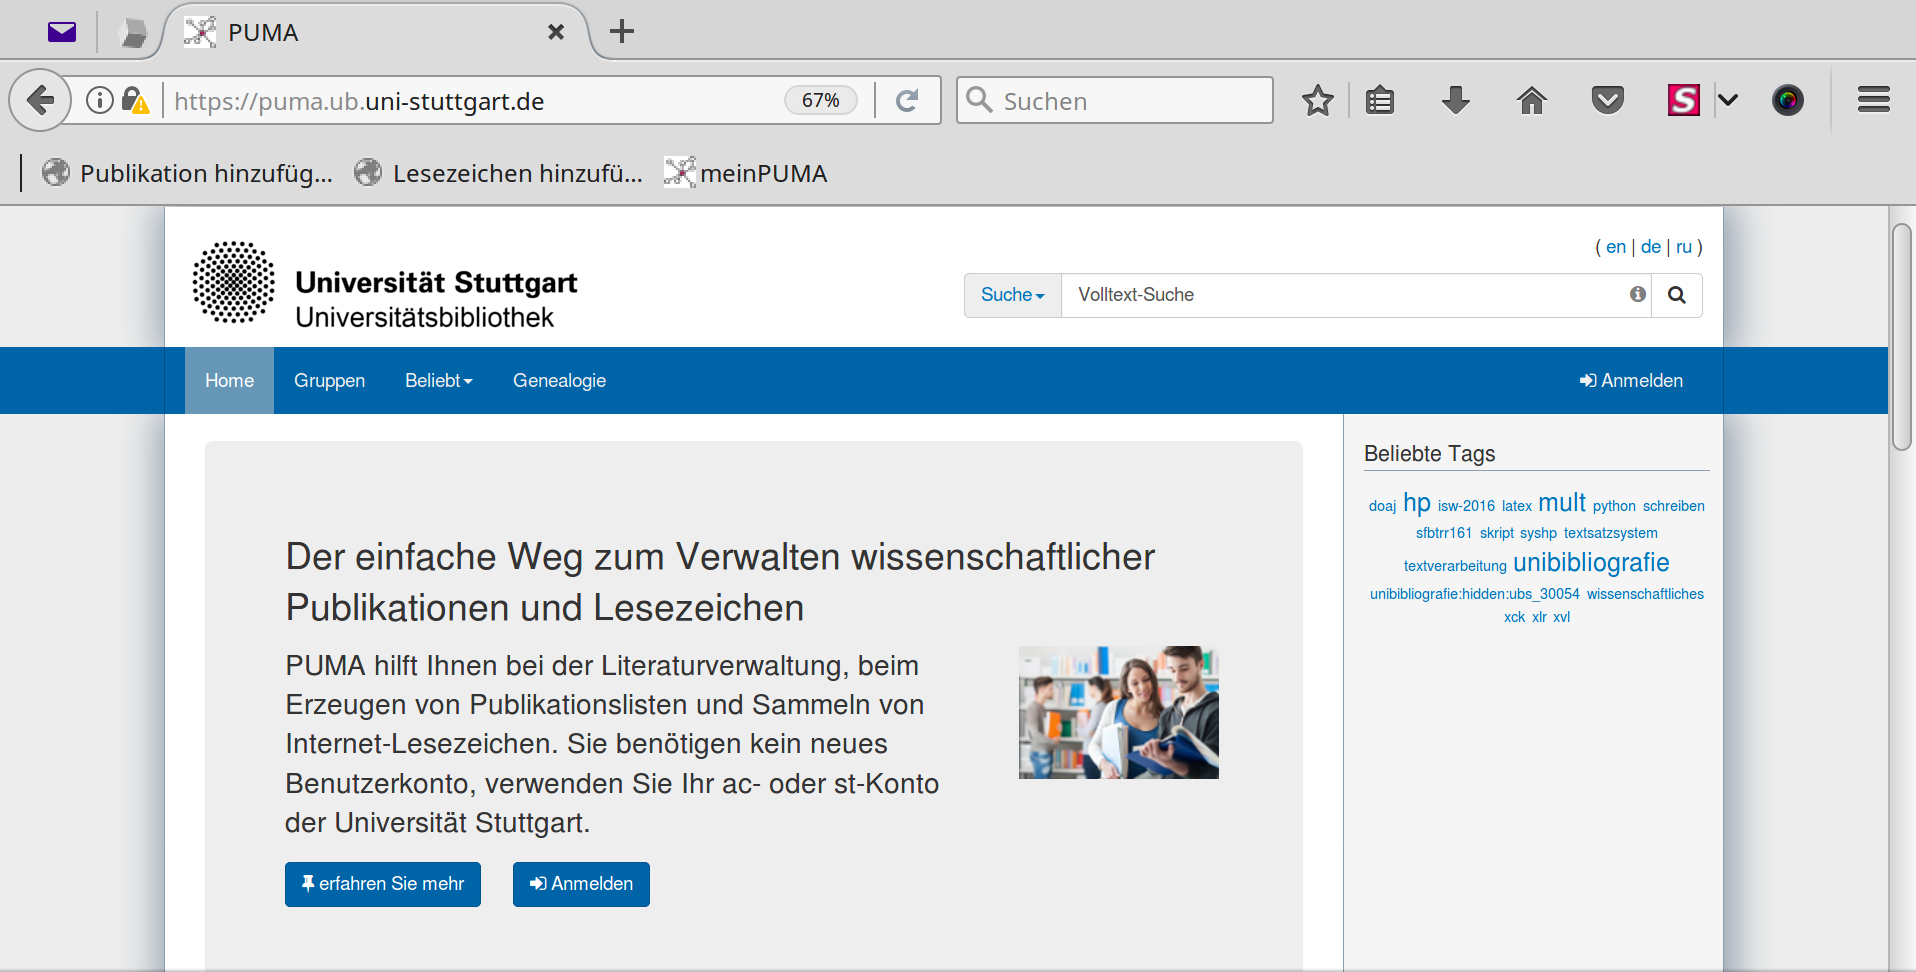
\includegraphics[width=10cm]{Bilder/Kapitel1/Startseite_PUMA}}
 \caption{Startseite PUMA}
 \label{figure001}
\end{figure}
\textbf{Vorab:} Sie benötigen ein st-, fn- oder ac-Konto der Universität Stuttgart.
\begin{enumerate}
    \item Rufen Sie die Anmeldeseite von PUMA auf:\newline \url{https://puma.ub.uni-stuttgart.de/}
    \item Geben Sie unter \enquote{Benutzername} Ihr ac- oder st-Konto der Universität Stuttgart ein (seltener ist das fn-Konto). 
    \item Unter  \enquote{Login} geben Sie Ihr Passwort ein. 
 \begin{figure}[h!]
 \centering
 \fbox{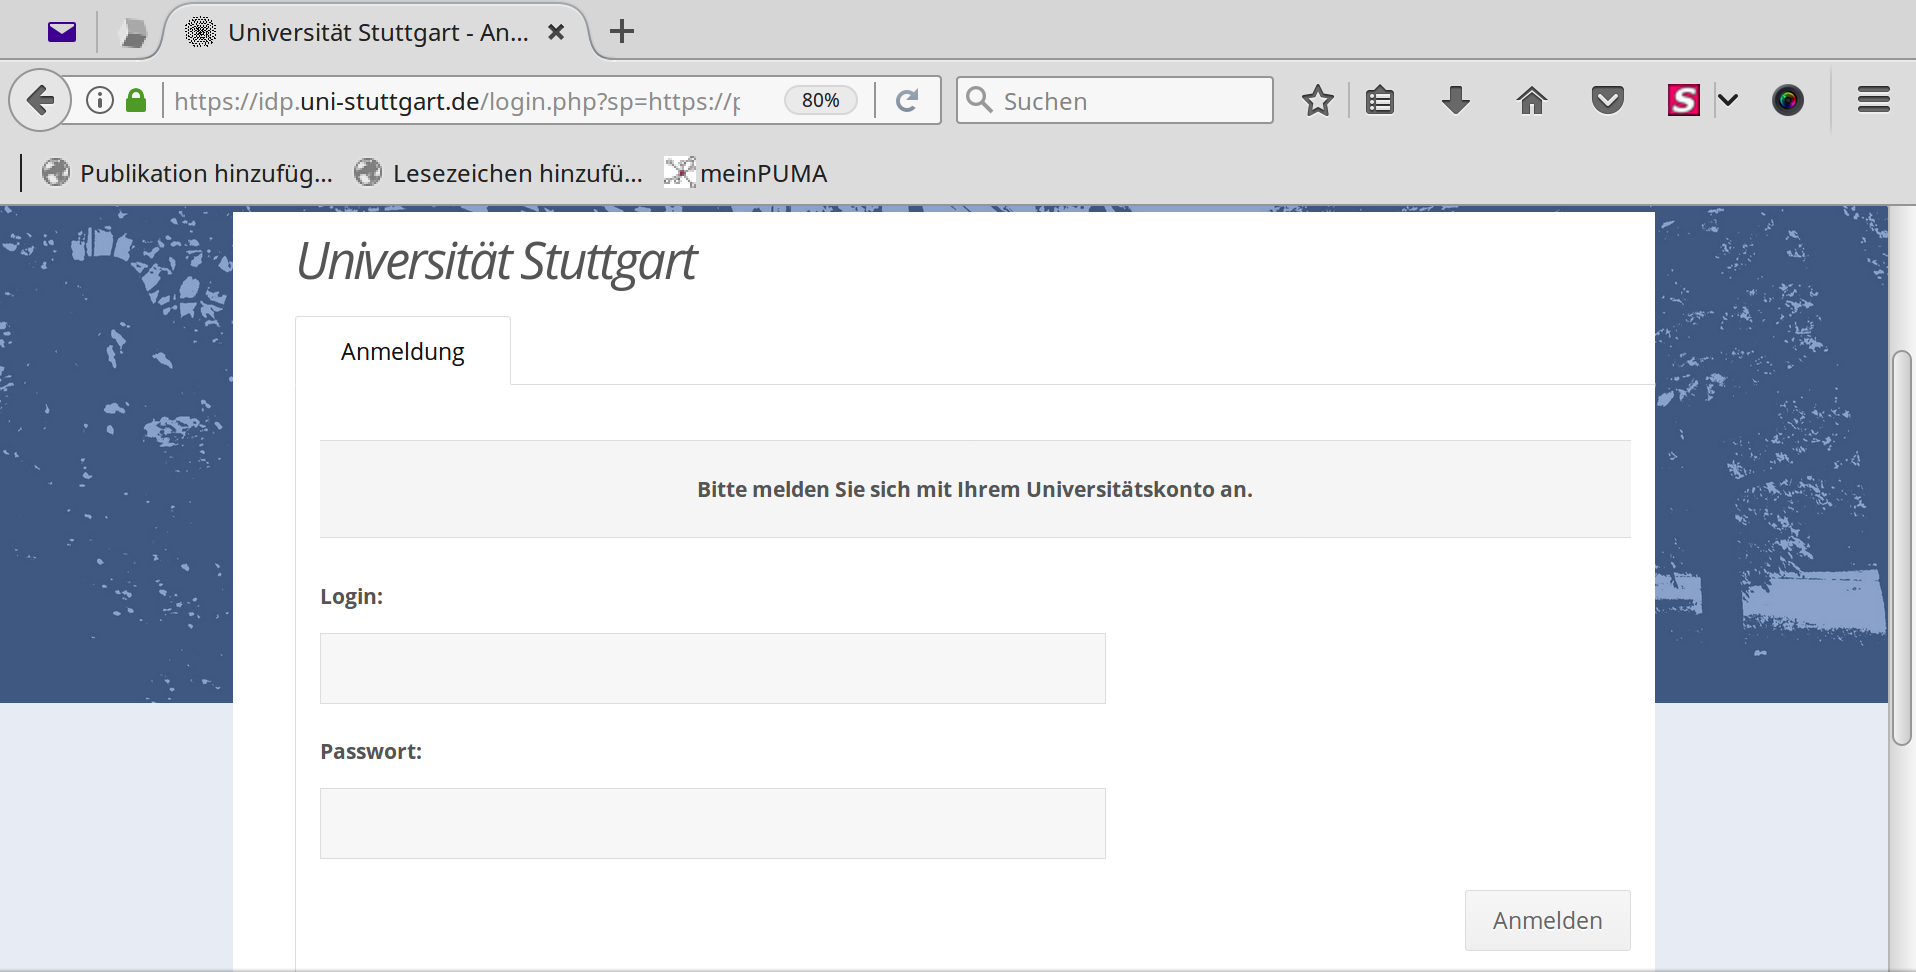
\includegraphics[width=9cm]{Bilder/Kapitel1/Anmeldung_bei_PUMA}}
 \caption{Anmeldung bei PUMA}
 \label{figure002}
\end{figure}  
    \item Klicken Sie auf \enquote{Anmelden}.
    \item Wenn Ihre Anmeldung erfolgreich war, zeigt Ihnen PUMA Ihre persönlichen Daten an. Überprüfen Sie die vorliegenden Daten, vergeben Sie einen Benutzernamen und klicken Sie anschließend auf \enquote{Registrieren}.
\end{enumerate}
Die Registrierung bei PUMA war erfolgreich. Ab sofort können Sie sich bei PUMA mit Ihrem Benutzerkonto anmelden. \newline
Bei der erstmaligen Anmeldung ist die Vergabe eines Benutzernamens erforderlich. Nur bei öffentlich geteilten Einträgen erscheint er bei den Publiaktionseinträgen in der Form @benutzername.
\section{Der PUMA-Blog}
Im Blog der Universitätsbibliothek Stuttgart (UB) ist neben allgemeinen Informationen zu der UB auch die Kategorie \enquote{PUMA} an wählbar (\url{http://blog.ub.uni-stuttgart.de/category/puma/}). Hier können die Nutzer sich über die aktuellen PUMA-Ereignisse einen Überblick verschaffen und werden über PUMA-Updates und neue Funktionen informiert.\newline
Mit Hilfe eines RSS-Feeds können Interessierte Informationen zu Server-Updates abonnieren. Über den Link: \url{http://blog.ub.uni-stuttgart.de/category/puma/feed/} werden die aktuellen Informationen angezeigt. Durch das Klicken auf \enquote{Jetzt abonnieren} öffnet sich ein Fenster, indem das Abonnieren nochmals bestätigt werden muss. Ab sofort können die Informationen über die Lesezeichen-Leiste angezeigt werden. 
\section{BibSonomy\index{BibSonomy}}
PUMA steht nur den Mitgliedern der Universität Stuttgart zu Verfügung, die über ein st-, fn- oder ac-Konto  verfügen. Für externe Nutzer der Universitätsbibliothek Stuttgart besteht die Möglichkeit das Muttersystem von PUMA, BibSonomy, zu nutzen. Beide Systeme verfügen über fast die gleichen Funktionen und Möglichkeiten seine Publikationen und Lesezeichen zu sammeln, verwalten und teilen. \newline
Die Anmeldung bei BibSonomy erfolgt über die Homepage \newline
\url{http://www.bibsonomy.org/?lang=de}.  

%\section{BibSonomy\index{BibSonomy} vs. PUMA}
%\suppressfloats[t]
\begin{table}[h!]
\tabulinesep=1.5mm
\begin{tabu}{|X[1.4,c]|X[2.2,m]|X[2,m]|} 
\tabucline[0.5pt]-\everyrow{\tabucline[0.5pt]-} 
\rowfont\bfseries
Unterschiede & PUMA \emph{Uni Stuttgart} & BibSonomy\\ \tabucline[1pt]-
\bfseries{Anmeldung}\strut & Nur möglich mit einem st-, fn- oder ac-Konto der Universität, mit dem sich die Nutzer authentifizieren.  & Für jeden frei zugänglich, ein Benutzerkonto muss selber angelegt werden. \\ 
\bfseries{Gruppen}\index{Gruppen} & Gruppen können jederzeit und selbständig gegründet werden. & Die Gründung einer Gruppe erfordert die Freigabe des BibSonomy-Admins. \\
\bfseries{OPUS}\index{OPUS} & Für die Zukunft geplant. Ermöglicht den Nutzern ein direktes Veröffentlichen auf dem Dokumentenserver OPUS. & \\ 
\bfseries{Unibibliografie}\index{Unibibliografie}& Die Publikationsmetadaten der Unibibliografie stehen zum Beispiel für Institutspublikationslisten zur Nachnutzung zur Verfügung.&\everyrow{} \\ \tabucline[1.0pt]-
\end{tabu}
\caption{Unterschiede zwischen PUMA und BibSonomy}
\end{table}
%\normalsize
\chapter{Schnelleinstieg}
\textit{Sammeln, Verwalten und teilen- so lautet die Devise.}
\section{Sammeln}
Bookmarks, bibliografische Daten und Volltexte kostenlos online speichern.\newline\newline
\textbf{Login}
\begin{itemize}
\item Sichere Verbindung: \url{https://puma.ub.uni-stuttgart.de/}
\item Angehörige der Universität Stuttgart: st- oder ac-Konto
\item Benutzername frei wählbar
\item Keine Lizenzgebühr
\end{itemize}
\textbf{Die ersten Schritte}
\begin{itemize}
\item Publikationen manuell eintragen oder per ISBN/DOI automatisch aus Datenbanken abrufen
\item Vergabe von Schlagwörtern (\enquote{Tags})
\item Mindestens ein \enquote{Tag} ist obligatorisch
\item Sichtbarkeit einstellen: privat, öffentlich oder für eine Gruppe
\item Ausführliche Anleitung: PUMA-Hilfe im Benutzermenü
\item Schulung für Einsteiger in der Universitätsbibliothek Stuttgart: \url{www.ub.uni-stuttgart.de/puma}
\end{itemize}
\textbf{Schlagworte (\enquote{Tags}) nutzen}
\begin{itemize}
\item Ausgabe von eigenen Publikationslisten per Systemtag \textit{myown}
\item Beliebige Sortiermöglichkeiten über Vergabe von Tags
\item Kombination von Tags zur Eingrenzung von Abfragen
\end{itemize}
\section{Verwalten}
Literaturlisten in unterschiedlichen Zitationsstilen erzeugen und exportieren.\newline\newline
\textbf{Import und Export von Daten}
\begin{itemize}
\item Vorhandene Publikationslisten importieren (BibTex oder Endnote-Formate)
\item Duplikatserkennung
\item Ausgabe von Literaturlisten in rund 7.500 Zitationsstilen
\item Oder individuelle Anpassung per Citation Style Language (CSL)
\item Export der Daten in Standardformate wie BibTex, Endnote oder XML
\item Viele Sortiermöglichkeiten nach Autor, Jahr, Dokumententyp u.a.
\end{itemize}
\section{Teilen}
Einträge per Plugin auf der Website veröffentlichen oder in Gruppen zugänglich machen.\newline\newline
\textbf{Soziale Funktion}
\begin{itemize}
\item Gruppen anlegen und Mitglieder verwalten
\item Sichtbarkeit auf die Gruppe beschränken
\item Gemeinsam Einträge bearbeiten (Community-Posts)
\item Freunden folgen und Einträge senden
\end{itemize}
\textbf{Plugin für OpenCMS der Universität Stuttgart}
\begin{itemize}
\item Verbindung mit dem PUMA-Benutzerkonto
\item Eigene Publikationslisten aus PUMA laden
\item Dokumentation im Typkatalog des TIK: \url{http://www.tik.uni-stuttgart.de/dienste/opencms/typkatalog/typ/PumaPublicationList/}
\end{itemize} 
\textbf{Typo3 Plugin}
\begin{itemize}
\item Verbindung mit dem PUMA-Benutzerkonto (Funktionsweise wie bei OpenCMS)
\item Eigene Publikationen aus PUMA laden und auf der eigenen Homepage veröffentlichen
\item Einfügen von eigenen CSL-Styles möglich
\end{itemize}
\chapter{Typische Anwendungsbeispiele}
\label{ch:typischeAnwendungsbeispiele}

\section{Institutspublikationsliste}
\label{sec:institutspublikationsliste}
Für die Veröffentlichung der Institutspublikationsliste (\autoref{subsec:opencms}) gibt es mehrere Möglichkeiten:
\begin{itemize}
\item Über die Gruppenfunktion (\autoref{sec:gruppen}) von PUMA: Diese Funktion ermöglicht, gemeinsam ein PUMA-Gruppenkonto zu verwalten. Gruppenadmins können Einträge bearbeiten, die Mitglieder der Gruppe an diese per Systemtag \textit{for:Gruppenname} (\autoref{systemtag}) geschickt haben. Damit ist der Eintrag im Besitz der Gruppe (\textit{@Gruppenname}) und des Gruppenmitglieds. Dieser Weg hat mehrere Vorteile: Zum einen können mehrere Personen Einträge bearbeiten. Zum anderen können in der Gruppe gleichzeitig auch Volltexte geteilt und Dubletten schneller erkannt werden. Aus dieser  Sammlung kann wiederum eine gemeinsame Institutspublikationsliste generiert werden.
\item Über ein Funktionskonto (fn-Konto): Das fn-Konto muss beim TIK über den Benutzerverwaltungsadministrator des Instituts beantragt werden. Dieses Konto funktioniert wie das st- oder ac-Konto, es hat den Vorteil, dass es nicht an eine Person gebunden ist und kann von verschiedenen Personen bedient werden. Aus der Sammlung kann eine gemeinsame Institutspublikationsliste generiert werden.
\item Über ein persönliches Konto werden die Publikationen gesammelt und in PUMA eingetragen. Aus der eigenen Sammlung wird dann die Institutspublikationsliste erstellt.
\end{itemize}
Scheidet ein Institutsmitarbeiter der Universität Stuttgart aus, bleibt sein Benutzerkonto bei PUMA auch nach Ausscheiden (\autoref{subsec:kontoAufloesen}) erhalten. Eine Authentifizierung ist nicht mehr möglich. Damit können diese Einträge vom Nutzer nicht mehr bearbeitet werden. Öffentlich geteilte Einträge des Ausgeschiedenen bleiben weiterhin nutzbar.\\
PUMA-Nutzer können ihr Konto jederzeit löschen (\autoref{subsec:kontoLoeschen}). Damit sind ihre Einträge ebenfalls gelöscht. Wenn die Publikationen am Institut erhalten bleiben sollen, kann ein anderer Nutzer des Instituts die Einträge vorher in die eigene Sammlung kopieren oder der Nutzer sendet per Systemtag \textit{for:Gruppenname} (\autoref{systemtag}) seine Publikationseinträge an eine Institutsgruppe. Die Pflege einer Institutspublikationsliste sollte aber möglichst von vorneherein über die Gruppenfunktion oder ein fn-Konto erfolgen.

\section{Eigene Publikationslisten verwalten und veröffentlichen}
\label{sec:eigenePublistenVerwalten}
Das Verwalten und Sortieren der eigenen Publikationen gestaltet sich mit PUMA einfach. Eigene  Publikationen können in PUMA gekennzeichnet werden. Nutzer können sich als Autoren der Publikation zu erkennen geben, indem beim Publikationseintrag ein Häkchen bei \textit{Ich bin (Mit-)Autor} gesetzt wird. Dies erzeugt automatisiert den Systemtag \textit{myown}. Systemtags sind \enquote{Tags}, die einheitlich definiert sind und weitere Funktionen beinhalten (\autoref{systemtag}).\\
Mit Hilfe des Plugins \enquote{Publikationsliste (aus BibSonomy/PUMA)} für OpenCms (\autoref{subsec:opencms}) kann die Publikationsliste auf einer Internetseite der Universität Stuttgart veröffentlicht werden. Das Plugin wird über das Zauberstab-Menü im Seiteneditor ausgewählt. Durch Verbindung mit dem PUMA-Benutzerkonto über den API-Schlüssel und Auswahl des eigenen Benutzerkontos werden alle Einträge, die mit diesem Konto bibliografiert wurden, angezeigt. Mit der Eingabe des \enquote{Tags} \textit{myown} wird nur die eigene Publikationsliste veröffentlicht.



\section{Materialsammlung für die Bachelorarbeit}
\label{sec:materialsammlungBachelorarbeit}
Um den Überblick über die Materialrecherche nicht zu verlieren, empfiehlt es sich spätestens bei der Bachelorarbeit den Umgang mit Literaturverwaltungsprogrammen zu üben. Bei der Literatursuche im Internet und in Bibliothekskatalogen unterstützt PUMA im Browser das Sammeln von Lesezeichen und Publikationen, ohne dass die Suche unterbrochen werden muss. Mit Unterstützung des PUMA-Add-ons für den Firefox (siehe \autoref{sec:addon}) oder Bookmarklet-Buttons (siehe \autoref{sec:button}) können diese in die eigenen PUMA-Sammlung eingetragen werden.\\
Es kommt nicht selten vor, dass einem bei der Menge an gesammelten Publikationen und Lesezeichen der Überblick verloren geht. In PUMA werden Materialsammlungen mit \enquote{Tags} (\autoref{subsec:tags}) strukturiert. Der Nutzer gibt diese \enquote{Tags} beim Eintragen mit an. Es gibt keine Beschränkung was die Anzahl der Tags betrifft. Die Vergabe der Tags erleichtert einem später das Finden der passenden Literatur zu einem Thema in der eigenen Sammlung. Wird nach einem Tag gesucht, zeigt PUMA alle Einträge mit diesem \enquote{Tag} an. So unterstützt PUMA das Entstehen einer strukturierten Literaturliste.\\
Im nächsten Schritt wird die Literatursammlung in Word importiert (siehe \autoref{sss:exportWord}). LaTeX-Nutzer können eine BibTeX-Datei aus PUMA exportiert. Beim Schreiben kann die Literatur dann referenziert und ein Literaturverzeichnis erzeugt werden.

\section{Aufbau}
\textit{Ein Blick genügt: Der Aufbau von PUMA ist durchschaubar. Durch ausprobieren lernt man ihn am Besten kennen.}
%Screenshot vom Hauptmenü
\subsection{Suchleiste}
Die Suche\index{Suche} bei PUMA bietet viele Möglichkeiten den Datensatz nach unterschiedlichen Informationen zu durchsuchen. Durch das Klicken auf den kleinen Pfeil neben \enquote{Suche}\index{Suche} erscheint ein Dropdown- Menü.  Der zu durchsuchende Datensatz wird durch anklicken ausgewählt. Anschließend wird der Suchbegriff in das weiße Feld daneben eingegeben. Durch das Klicken auf \enquote{Suche} oder \enquote{Enter} gibt PUMA in wenigen Sekunden die entsprechende Ergebnisse aus.

\begin{figure}[ht]
 \centering
 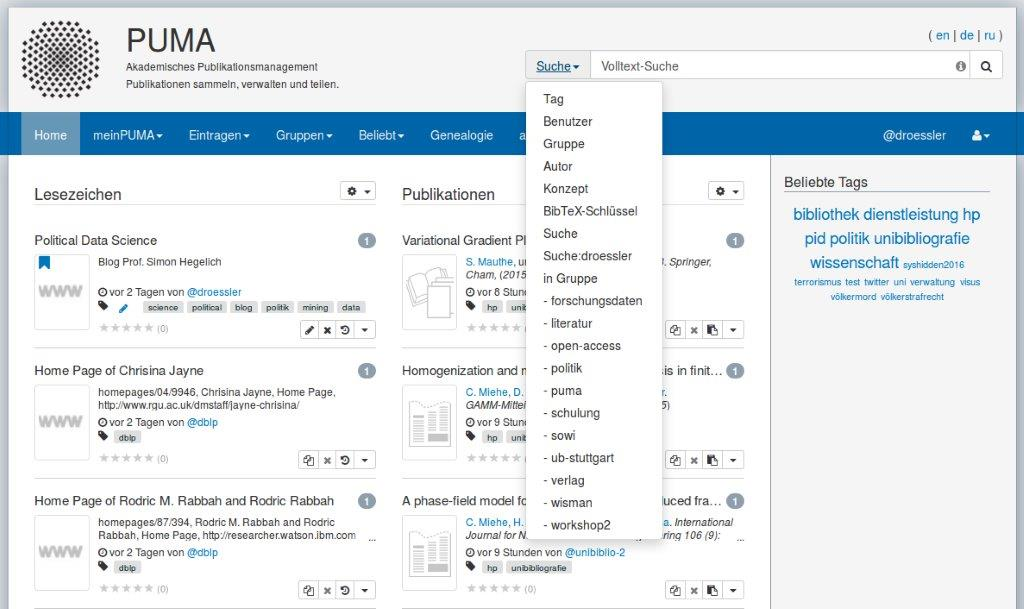
\includegraphics[scale=0.25]{puma-003.png}
 \caption{Suchleiste}
 \label{figure3}
\end{figure}  

\subsection{Spracheinstellung}
Hier haben Sie die Möglichkeit zwischen den drei verfügbaren Sprachen\index{Sprachen} in PUMA zu wechseln. Es gibt die Möglichkeiten zwischen Englisch (en), Deutsch (de) und Russisch (ru) zu wählen.
\newline
\begin{shaded}
\centering
\textbf{TIPP:} Um die Sprache für die Seite festzulegen, sodass diese bei jedem neuen Besuch bei PUMA gleich ist, müssen Sie dies in den Einstellungen festlegen. Dorthin gelangen Sie über das Personensymbol rechts im Hauptmenü. Sie klicken auf die schwarzen Einstellungs-Zahnräder und die Seite mit den Einstellungen öffnet sich. Anschließend klicken Sie auf den Reiter \enquote{Einstellungen}. Auf der erscheinenden Seite können Sie nun die gewünschte Sprache festlegen und müssen anschließend auf \enquote{Layout speichern} die Änderung bestätigen.
\end{shaded}
\subsection{Linkes Hauptmenü}
Das Hauptmenü stellt die wichtigsten Funktionen von PUMA bereit. Es ist zu beachten, dass sich einige Einstellungen unterscheiden, da es bei PUMA die Unterscheidung zwischen einfachen Funktionen\index{Funktionen!Einfache} und erweiterten Funktionen\index{Funktionen!Erweiterte} gibt (vgl. Kapitel 4.3: Freischalten von erweiterten Funktionen), dies betrifft vor allem den unten genannten Punkt \enquote{Mein PUMA}. 
\subsubsection{Home\index{Home}}
Damit gelangen Sie zur Startseite und erhalten einen Überblick über Publikationen und Lesezeichen die vor kurzer Zeit eingetragen wurden.
\subsubsection{Mein PUMA\index{Mein PUMA}}
Es ist zu beachten, dass sich einige Einstellungen unterscheiden, da es bei PUMA die Unterscheidung zwischen einfachen Funktionen\index{Funktionen} und erweiterten Funktionen gibt. Durch das Freischalten der erweiterten Funktionen kommen weitere Funktionen hinzu.
\begin{enumerate}
    \item Einfache Funktion\index{Funktionen!Einfache}:
    \begin{itemize}
        \item meine Einträge\index{Einträge}: Hier gelangen Sie zu dem eigenen Publikations- und Lesezeichenverzeichnis, das Sie sich angelegt haben.
        \item Diskutierte Einträge\index{Einträge!Diskutierte}: Hier finden Sie alle Publikationen und Lesezeichen, die Sie selber bewertet haben. Ebenso werden Kommentare und Rezessionen von anderen Nutzern zu Ihren Publikationen hier angezeigt.
    \end{itemize}
    \item Erweiterte Funktionen\index{Funktionen!Erweiterte}:
    \begin{itemize}
        \item Private Einträge\index{Einträge!Privat}: Damit gelangen Sie zu Ihren Einträgen, die nur für Sie sichtbar sind. 
        \item Einträge für Freunde\index{Einträge!Freunde}: Zeigt die Einträge, die nur Sie selber und Ihre Freunde sehen können.
        \item Dokumente\index{Dokumente}: Wenn Sie Ihren Einträgen Dokumente (z.B. eine PDF) angehängt haben, können Sie hier eine Übersicht über die angehängten Dokumente sehen.
        \item Duplikate\index{Duplikate}: Zeigt Ihnen die Einträge, die wahrscheinlich Duplikate sind. So können Sie ihre Literaturliste ganz einfach bereinigen. 
        \item Konzepte\index{Konzepte}: Konzepte ermöglichen es Ihnen mehreren Schlagwörtern zu gruppieren. %vllt noch mehr
        \item Lebenslauf\index{Konzepte}: Hier können Sie Ihre persönlichen Daten hinterlegen, welche für andere Nutzer in PUMA sichtbar sind.
        \item Publikationen durchstöbern: Mit dieser Funktion können Sie Ihre eigenen Lesezeichen/Publikationen durchstöbern. Sie erhalten so einen schnellen Überblick über den eigenen Literaturbestand. (vgl. Kapitel 4.5)
        \item BibTex\index{BibTex} exportieren: Exportiert Ihre Daten in das BibTex-Format.
    \end{itemize}
\end{enumerate}
\subsubsection{Eintragen}
\begin{enumerate}
    \item Lesezeichen eintragen\index{Lesezeichen!Eintragen}: Fügen Sie ein neues Lesezeichen Ihrer Sammlung hinzu. (vgl. Kapitel 3.2) 
    \item Publikation eintragen\index{Publikationen!Eintragen}: Fügen Sie ein neue Publikation Ihrer Sammlung hinzu. (Vgl. 3.3)
    \item Lesezeichen importieren\index{Lesezeichen!Import}: Importieren Sie Lesezeichen aus Ihrem Browser oder Ihren Delicious Daten.
\end{enumerate}


\subsubsection{Gruppen}
Zeigt Ihnen die Funktionen zu Gruppen\index{Gruppen} an, sowie die Gruppen in denen Sie Mitglied sind.
\begin{enumerate}
    \item Alle Gruppen: Verschafft Ihnen einen Überblick über alle existierenden Gruppe bei PUMA.
    \item Eine neue Gruppe erstellen: Bietet Ihnen die Möglichkeit eine eigene Gruppe zu erstellen.
\end{enumerate}
\subsubsection{Beliebt\index{Beliebt}}
Ermöglicht Ihnen, die derzeitig beliebtesten Einträge bei PUMA zu durchforsten.
\begin{enumerate}
    \item Einträge: Zeigt die beliebtesten Einträge an.
    \item Tags: Zeigt die beliebtesten Tags in einer Schlagwortwolke an. Je größer ein Tag ist, desto beliebter ist er.
    \item Autor: Zeigt die beliebtesten Autoren an.
    \item Konzepte: Zeigt die beliebtesten Konzepte und deren Zuordnungen an. 
    \item Diskussionen: Zeigt Lesezeichen und Publikationen an, über welche viel diskutiert wurde. 
\end{enumerate}
\subsubsection{Genealogie}

%InHALT
\subsection{Rechtes Hauptmenü}
\subsubsection{@username\index{@username}}
Über diesen Button gelangen Sie zu Ihrer Publikations- und Lesezeichensammlung. 
\subsubsection{Das Personensymbol}
\begin{enumerate}
    \item Eingang\index{Eingang}: Dies ist Ihr Lesenzeichen-/Publikations-Posteingang. Freunde/ Gruppen können Ihnen Publikationen und Lesezeichen zuschicken, diese Eingänge landen dann hier.
    \item Ablage\index{Ablage}: In der Ablage können Sie aktuelle Literaturlisten zusammenstellen. \hyperlink{Ablage}{(vgl. Kapitel 3.8)}
    \item Freunde\index{Freunde}: Hier erhalten Sie einen Überblick über Ihre Freunde. 
    \item Tags bearbeiten\index{Tags!Bearbeiten}: Hier können Sie Tags und Konzepte überarbeiten, beispielsweise alte Tags durch neue ersetzten. Genauere Informationen zu Tags vgl. Kapitel 3.5 .
    \item Einstellungen\index{Einstellungen}: Zeigt Ihre persönlichen Benutzereinstellungen an. Sie können hier Ihr Profil, die allgemeinen Einstellungen, Ihren Lebensauf sowie Einstellungen zu Gruppen ändern.
    \item Weblog\index{Weblog}: Leitet Sie zu dem Weblog \footnote{\url{http://blog.ub.uni-stuttgart.de/category/puma/}} von PUMA weiter.
    \item Hilfe\index{Hilfe}: Damit gelangen Sie zur Online-Hilfe.
    \item Abmelden\index{Abmelden}: Wenn Sie PUMA verlassen wollen melden Sie sich hier ab. 
\end{enumerate}

\textbf{Der PUMA-Aufbau im Überblick}
\small
\begin{longtable}{|c|m{3cm}|m{3cm}|m{3cm}|}\hline 
\bfseries Hauptmenü&\bfseries Untermenü&Reiter &\bfseries Rubrik\\  \hline
Eintragen&Lesezeichen eintragen &- &-\\ \cline{2-4}
&Publikation eintragen &Per Hand& Trage Sie Ihre Publikation hier ein\\\cline{3-4}
&&BibTex/EndNote-Schnipsel& Tragen Sie hier Ihre BibTex- oder EndNote-Schnipsel ein\\ \cline{4-4}
&&& Einstellungen\\ \cline{3-4}
&&Datei hochladen& Laden Sie ihre BibTex- oder EndnOte-Datei hier hoch\\ \cline{4-4}
&&&Einstellungen\\ \cline{3-4}
&&ISBN/DOI& ISBN\\ \cline{4-4}
&&& ISSN \\ \cline{4-4}
&&&DOI\\ \cline{3-4}
&&Code scannen&-\\ \cline{2-4}
&Lesezeichen importieren& &Importieren Sie Ihre Lesezeichen aus Ihrem Browser\\ \cline{4-4}
&& & Importiern Sie Ihre Delicious Daten\\ \hline 
Gruppen&Alle Gruppen& Gruppen von A-Z &-\\ \cline{2-4}
&Gruppen, in denen der Nutzer Mitglied ist& Einträge &-\\\cline{3-4}
&&Interessant für &- \\ \cline{3-4}
&&Sichtbar&-\\ \cline{3-4}
&&Dokumente&-\\ \cline{3-4}
&&diskutierte Einträge&-\\ \cline{3-4}
&&Einstellungen& Gruppeneinstellungen und Mitgliederliste\\ \cline{2-4}
&Eine neue Gruppe erstellen&-&-\\ \hline
Personensymbol&Eingang&-&-\\ \cline{2-4}
&Ablage&-&-\\ \cline{2-4}
&Freunde&Ihre Freunde&- \\ \cline{3-4}
&&Sie sind ein Freund von&- \\ \cline{2-4}
&Tags bearbeiten&-&Umbenennen/ Ersetzen von Tags\\ \cline{4-4}
&&&Subtags zu Konzepten hinzufügen\\ \cline{4-4}
&&&Subtags von Konzept löschen\\ \cline{2-4}
&Einstellungen&Mein Profil&Allgemeine Informationen\\ \cline{4-4}
&&&Kontakt\\ \cline{4-4}
&&&Über mich\\ \cline{4-4}
&&&Ein Bild für meinen Lebenslauf\\\cline{3-4}
&&Einstellungen&Layouts Ihrer Tagbox und Ihrer Eintragsbilder\\\cline{4-4}
&&&API\\\cline{4-4}
&&&Logging und Löschen\\\cline{4-4}
&&&Passwort ändern\\\cline{4-4}
&&&Mein Konto löschen\\\cline{3-4}
&&JabRef Layout-Datei&-\\\cline{3-4}
&&Lebenslauf& Lebenslauf editieren\\\cline{4-4}
&&&layout editieren\\ \cline{4-4}
&&&Vorschau wird erzeugt\\\cline{3-4}
&&OAuth-Consumers&- \\\cline{3-4}
&&Gruppen&Eine neue Gruppe erstellen\\\cline{4-4}
&&&Gruppen\\\cline{2-4}
&Einstellungen&Synchronisation&-\\\cline{2-4}
&Weblog&-&-\\\cline{2-4}
&Hilfe&-&-\\\cline{2-4}
&Abmelden&-&-\\\hline
\end{longtable}
\normalsize

\subsection{Inhaltsbereich}
Hier sehen Sie die aktuellsten Lesezeichen und Publikationen von Ihnen und anderen Nutzern. 
\subsection{Beliebte Tags}
Zeigt Ihnen die beliebtesten Tags\index{Tags} an. Sie können zwischen der Wolken-oder Listen-Ansicht wählen.
\chapter{Basics}
\label{ch:basics}
\textit{Man muss kein Computerexperte ein, um mit PUMA arbeiten zu können. Wie alles genau funktioniert erfahren Sie in diesem Kapitel.}
\section{Einstellungen}
\label{sec:einstellungen}
Zu den Einstellungen\index{Einstellungen} gelangen Sie über das Personensymbol. Klicken Sie im Dropdown-Menü auf \enquote{Einstellungen}. In den Einstellungen können Sie zwischen unterschiedlichen Reitern wählen:\newline \newline
\textbf{Mein Profil\index{Mein Profil}} \newline
Unter diesem Reiter können Sie alle Einstellungen in Bezug auf Ihr Profil vornehmen.\newline \newline 
\textbf{Einstellungen} \newline
In den \enquote{Einstellungen} können Sie das Layout Ihrer Tagwolken festlegen, Ihr Passwort ändern oder Ihr PUMA-Konto löschen. Unter der Rubrik \enquote{Bevorzugte Exportformate} können Sie die Zitationsstile auswählen, die Ihnen auf den Publikationsseiten angezeigt werden sollen. So werden die Zitiervorlagen nach Ihren Vorlieben und Anforderungen angepasst.\newline Außerdem finden Sie unter diesem Reiter alle nötigen Informationen zu Ihrem API-Key.\newline \newline
\textbf{JabRef Layout-Datei\index{JabRef! Layout-Datei}}\newline
In diesem Reiter können Sie Ihre JabRef Layout-Dateien hochladen, um Ihre Publikationsliste nach Ihren eigenen Wünschen darzustellen.  \newline \newline
\textbf{Lebenslauf\index{Lebenslauf}} \newline
Dieser Reiter ermöglicht Ihnen Ihren Lebenslauf zu bearbeiten. \newline \newline
\textbf{OAuth-Consumers\index{OAuth-Consumers}} \newline
Hier sind alle OAuth-Consumer aufgelistet, die eine Autorisierung auf Ihren PUMA Account von Ihnen bekommen haben. \newline \newline
\textbf{Gruppen\index{Gruppen}}\newline
Sie erhalten einen Überblick über alle Gruppen, in denen Sie Mitglied sind. Sie können auch eine neue Gruppe anlegen. \newline \newline
\textbf{Synchronisation} \newline
Mit Hilfe der Synchronisation können Sie Ihre Lesezeichen und Publikationen zwischen zwei Systemen synchron halten.  
\section{CV/Lebenslauf}
\label{sec:cv}
Ihr Lebenslauf ermöglicht anderen Benutzern Sie und Ihre Arbeiten kennen zu lernen. Die Daten, die Sie in Ihr Profil schreiben sind für alle PUMA-Nutzer sichtbar. Für Ihr Profil können Sie entweder vordefinierte Layouts benutzen oder selbst ein Layout mit Hilfe der MediaWiki-Syntax\footnote{\url{https://en.wikipedia.org/wiki/Help:Wiki_markup}} definieren. 
\begin{figure}[h!]
 \centering
 \fbox{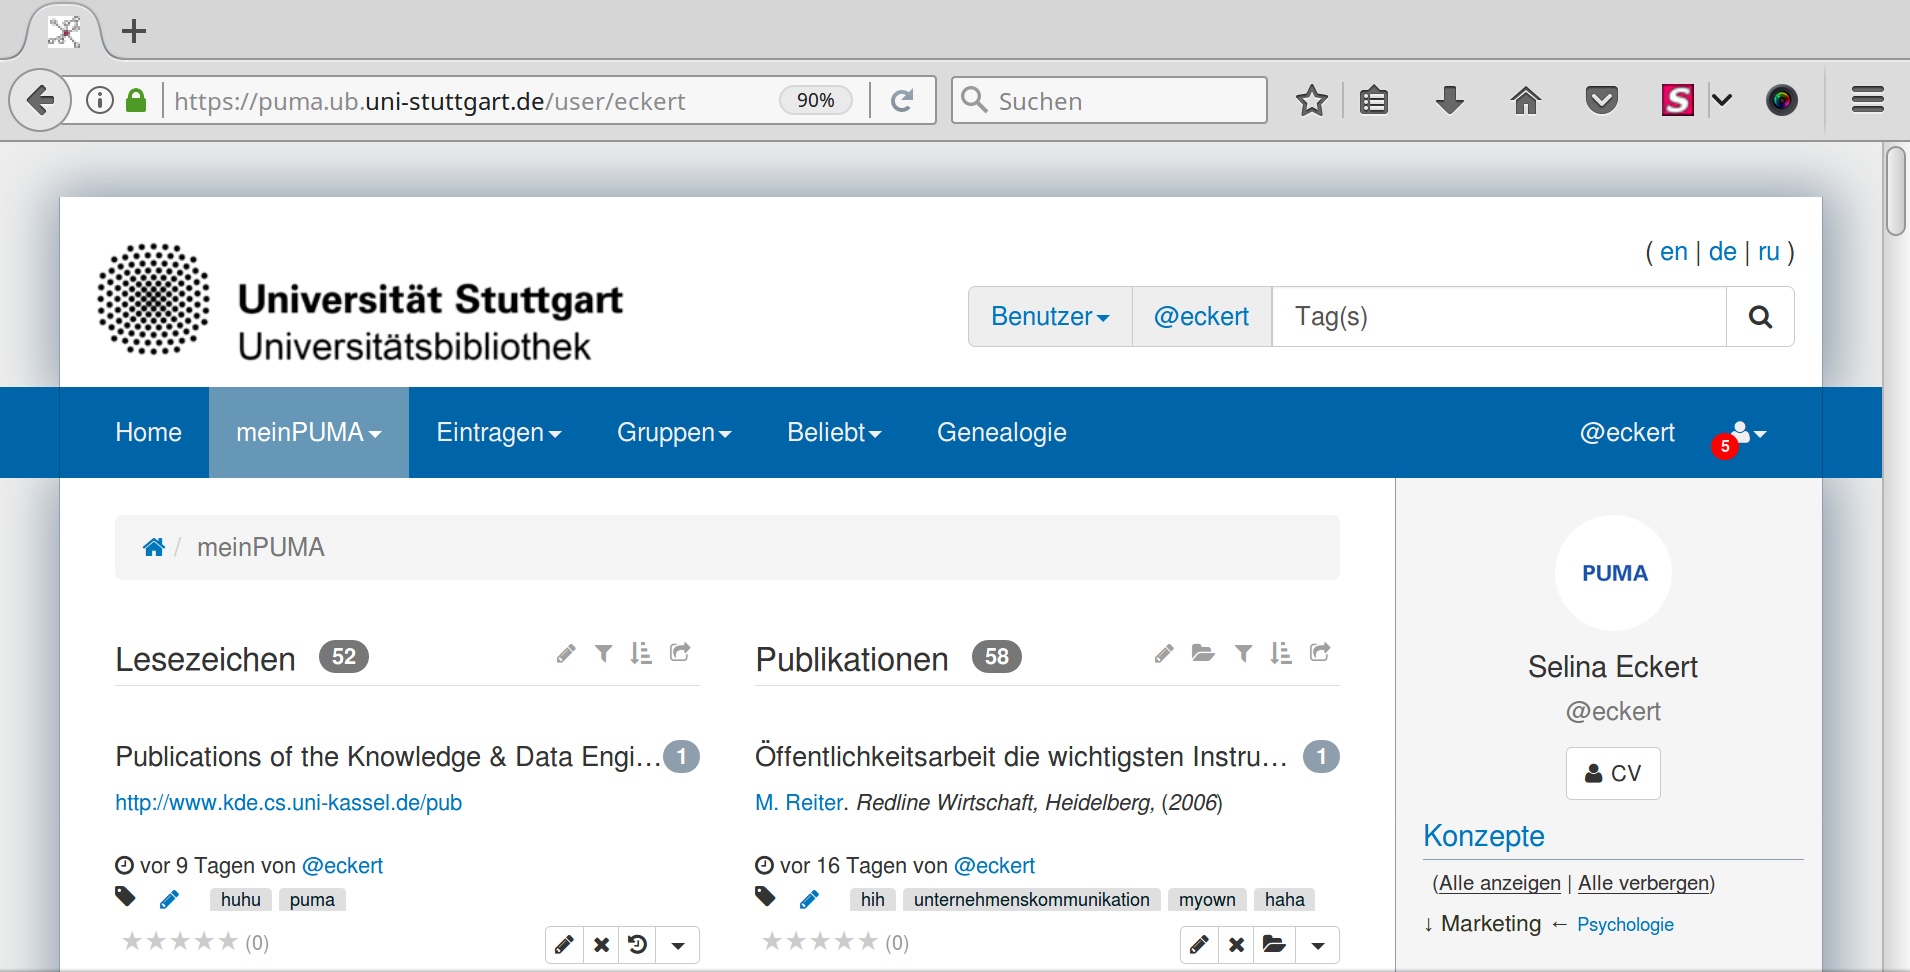
\includegraphics[width=11cm]{Bilder/Kapitel5/CV_Benutzerkonto}}
 \caption{Das Benutzerkonto}
 \label{fig:benutzerkonto}
\end{figure}  
Lebenslauf bearbeiten\index{Lebenslauf!bearbeiten}: 
\begin{enumerate}
    \item Klicken Sie auf Ihren Benutzernamen (@username).
    \item Klicken Sie rechts neben Ihrem Profilbild auf den CV-Button.
    \item Ihr Lebenslauf öffnet sich (Ansicht: So wie ihn andere Nutzer sehen).
    \item Um den Lebenslauf zu bearbeiten klicken Sie auf das schwarze Zahnrad neben \enquote{Curriculum Vitae}.
    \item Klicken Sie anschließend im Untermenü auf \enquote{Lebenslauf bearbeiten}. Sie können nun ein vordefiniertes Layout auswählen oder selbst ein Layout mit der MediaWiki-Syntax definieren.
\end{enumerate}
\textbf{Alternativer Weg:} 
\begin{enumerate}
    \item Klicken Sie auf das Personensymbol. Es öffnet sich ein Untermenü.
    \item Klicken Sie im Untermenü auf \enquote{Einstellungen}.
    \item Eine neue Seite öffnet sich. Klicken Sie auf den Reiter \enquote{Lebenslauf}. Sie können nun ein vordefiniertes Layout auswählen oder selber ein Layout mit der MediaWiki-Syntax definieren.
\end{enumerate}
%\begin{wrapfigure}{l}{5cm}
\begin{mdframed}[style=tipp]\texttt{Wenn Sie zwischen den vordefinierten Layouts wechseln, geht Ihr selbst definiertes Layout verloren.} 
\end{mdframed}
%\end{wrapfigure}
\begin{figure}[h!]
 \centering
 \fbox{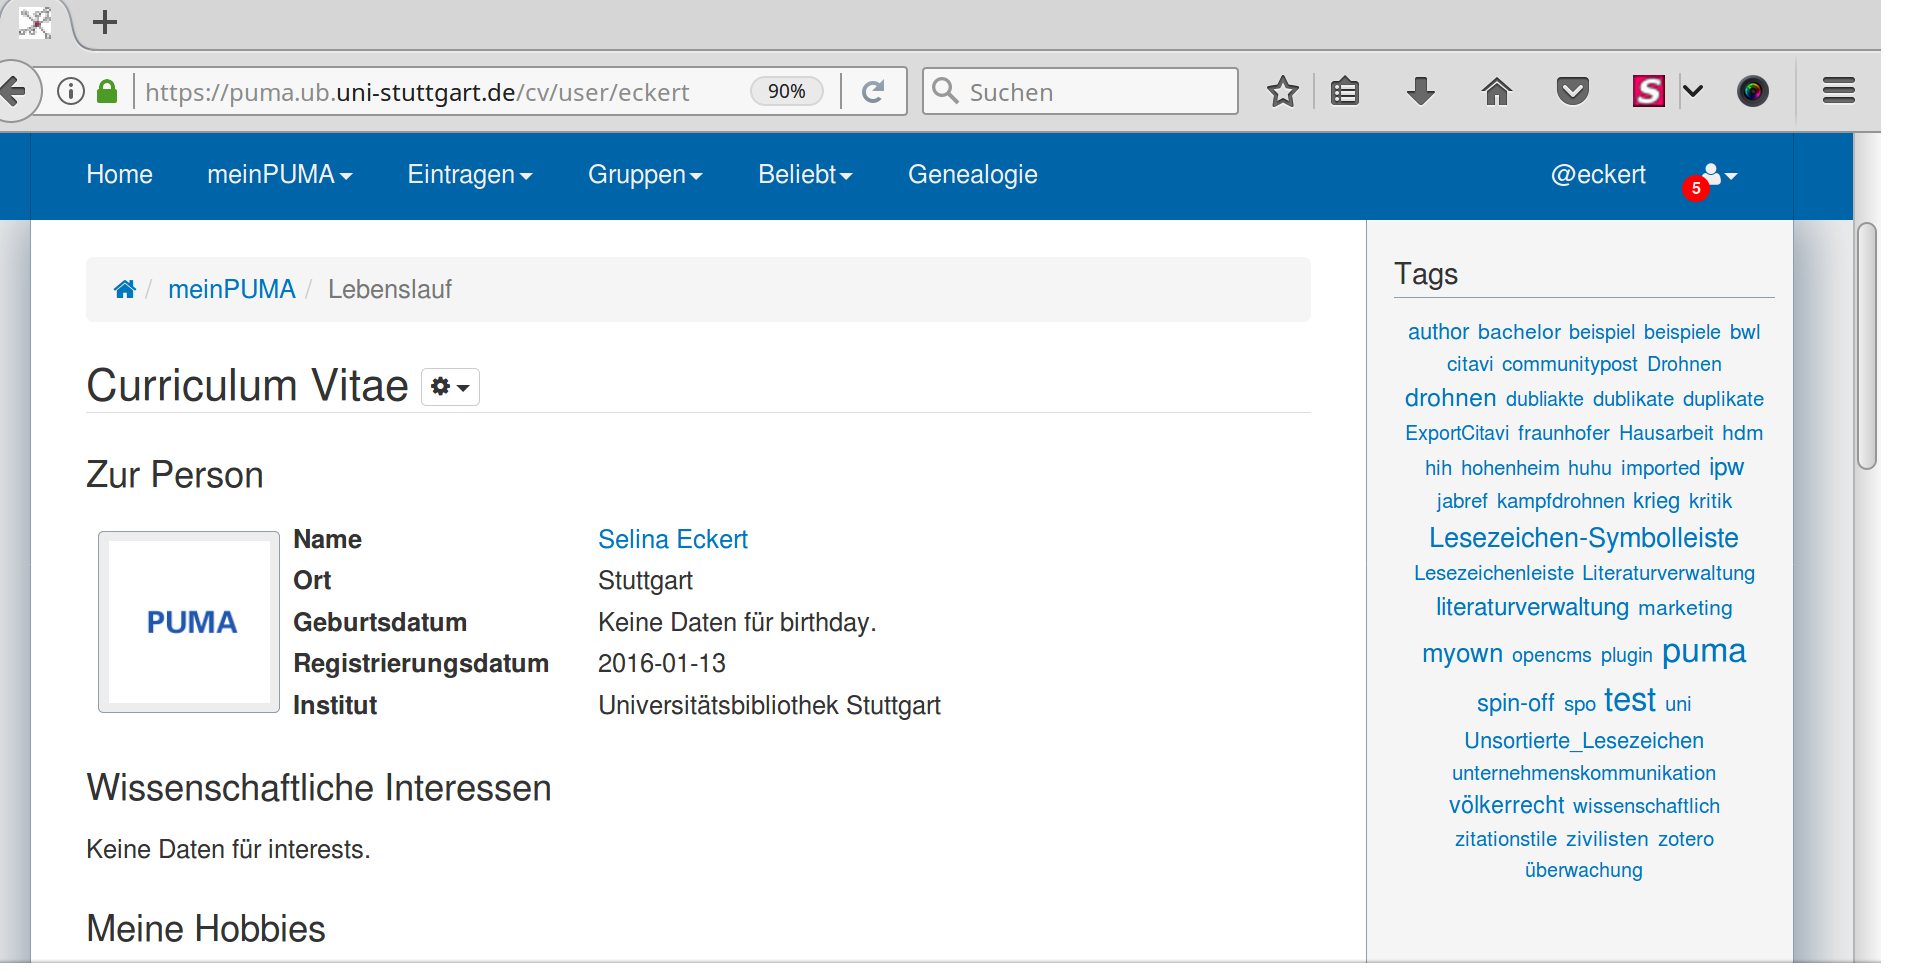
\includegraphics[width=11cm]{Bilder/Kapitel5/CV_Seite}}
 \caption{Curriculum Vitae-Seite}
 \label{fig:curriculumVitaeSeite}
\end{figure}  
\hypertarget{Eigenes Layout}{Eigenes Layout\index{Lebenslauf!Eigenes Layout}:}
\newline
Um sich selbst ein Layout zu definieren, müssen Sie die MediaWiki-Sytax verwenden. Um Zeit zu sparen bieten wir Ihnen einige XHTML-Tags an: % Tabelle % ist XHTML bei wiki???
\newline
Für die Tags \textit{<publications />} und \textit{<bookmarks />} können Sie außerdem eigene Tags als Ressourcenselektoren benutzen, wenn Sie tags=\enquote{tag1 tag2 (...)} als Attribute anfügen. Beispielsweise liefert \textit{<publications tags=\enquote{data mining} />} alle Ihre Publikationen, die Sie sowohl mit data als auch mit mining getagged haben. 
\begin{figure}[h!]
 \centering
 \fbox{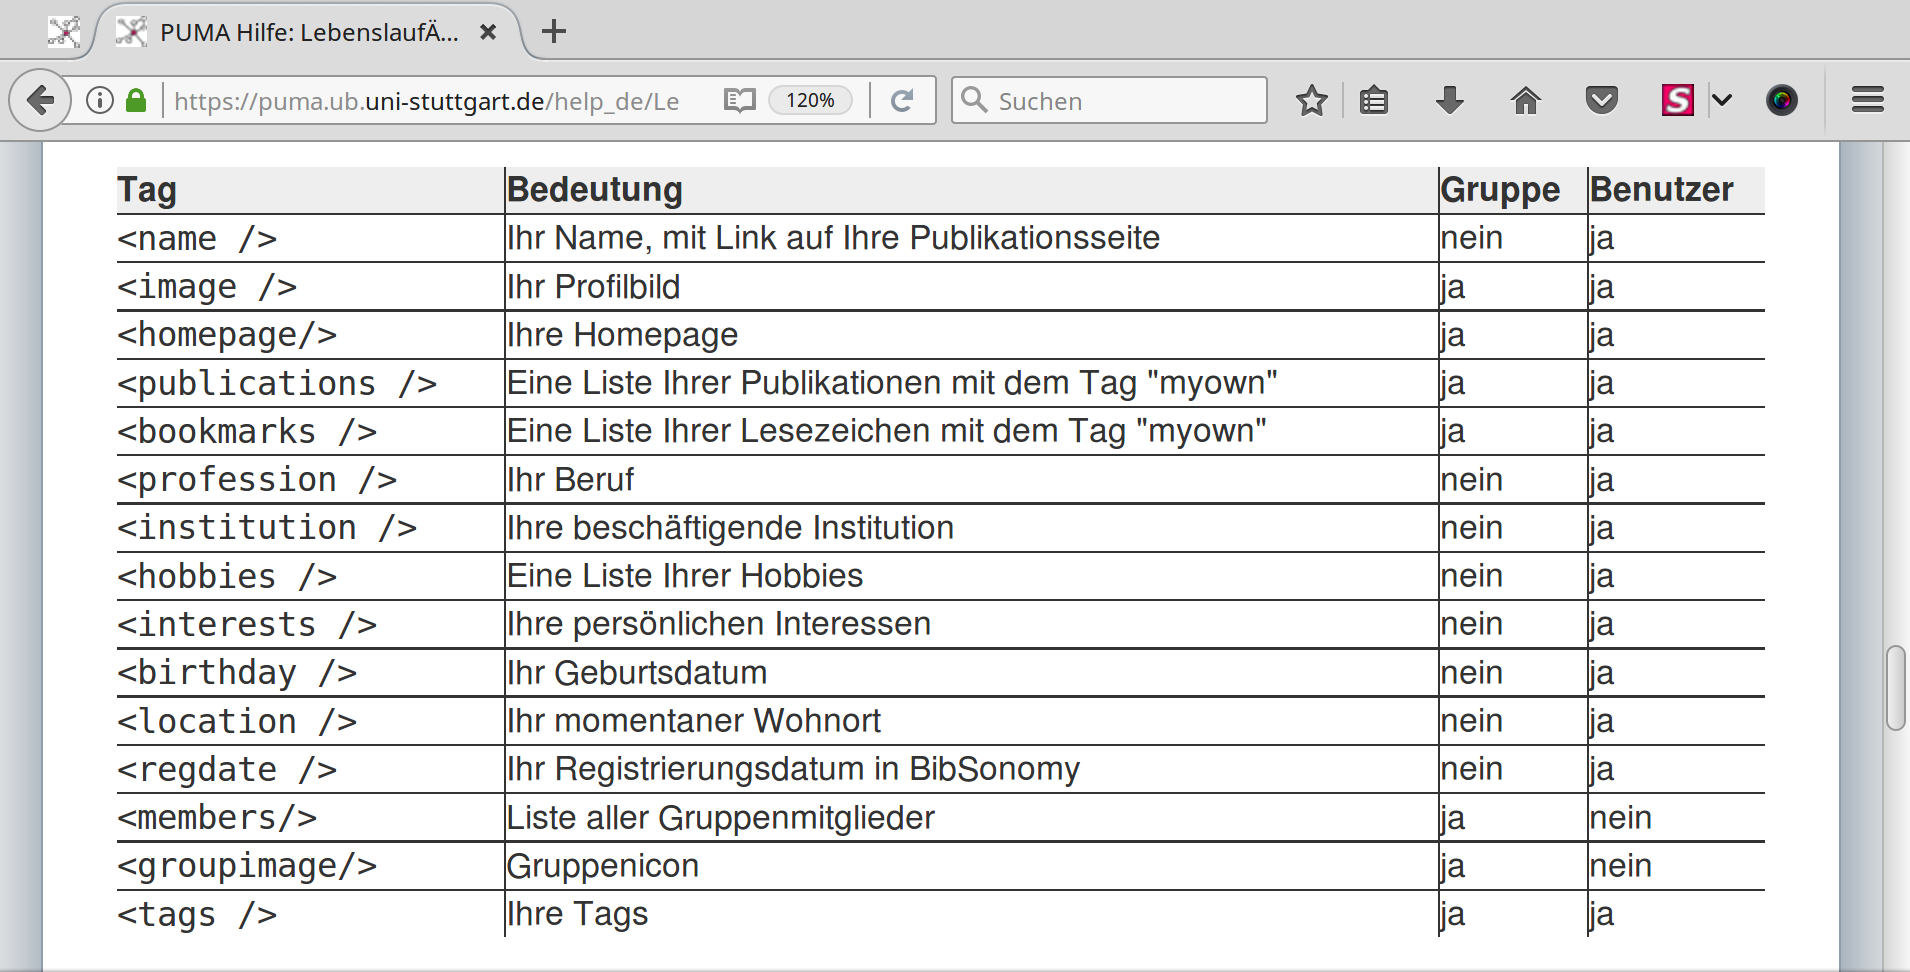
\includegraphics[width=11cm]{Bilder/Kapitel5/xhtml_tags}}
 \caption{XHTML-Tags}
 \label{fig:xhtmlTags}
\end{figure}  
\section{Publikationen}
\label{sec:publikationen}
Grundlagen:
\newline
Unter Publikationen\index{Publikationen} versteht man in PUMA alle Arten von Dokumenten (Artikel, Monografie, usw.). Sie können eigene oder fremde Publikationen (z.B. als Basis für eine Literaturrecherche) mit PUMA erstellen/~verwalten/~recherchieren. 
\begin{figure}[h!]
 \centering
 \fbox{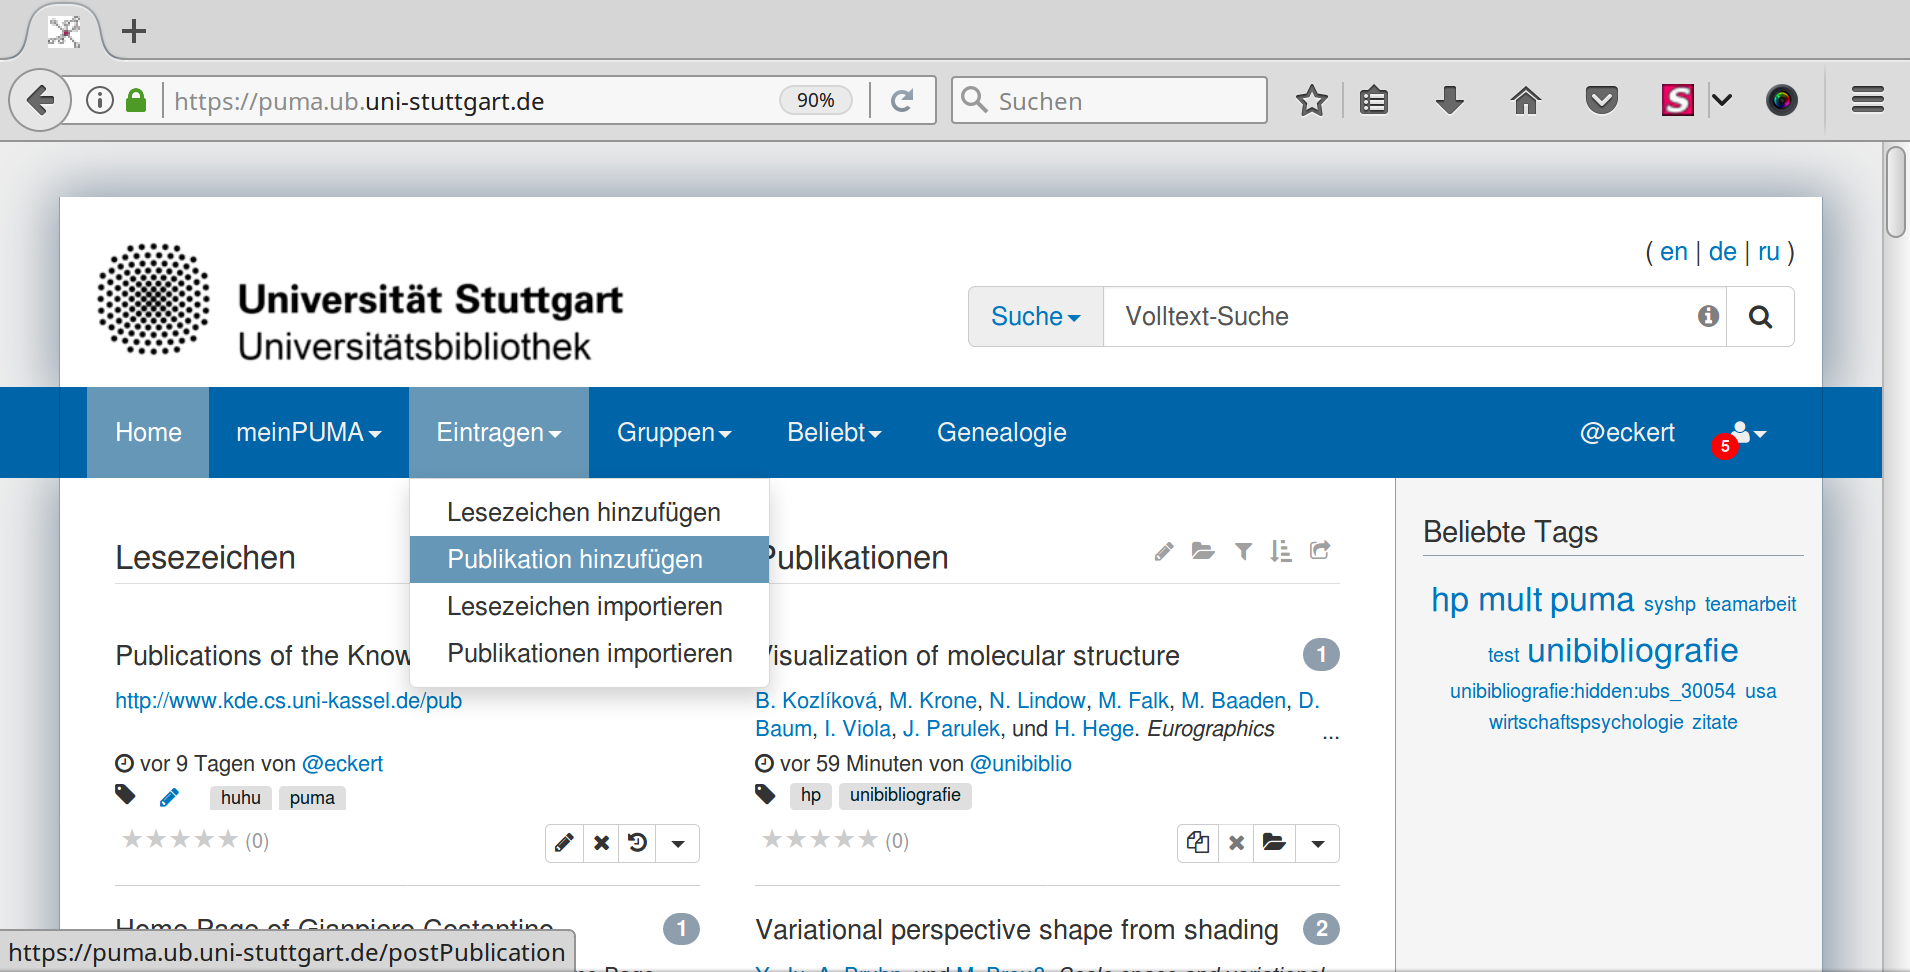
\includegraphics[width=11cm]{Bilder/Kapitel5/Publikation_eintragen}}
 \caption{Publikationen eintragen}
 \label{fig:publikationenEintragen}
\end{figure}  
Publikationen hinzufügen\index{Publikationen!hinzufügen}:
\begin{enumerate}
    \item Klicken Sie auf den Menüpunkt \enquote{Eintragen} im Hauptmenü. Ein Untermenü klappt auf.
    \item Klicken Sie im Untermenü auf \enquote{Publikation hinzufügen}.
    \item Sie können nun direkt in das Textfeld den Titel oder die ISBN/~ISSN/~DOI der Publikationen eingeben und PUMA zeigt Ihnen die entsprechenden Metainformationen der Publikation an. Neben dieser Weg bietet PUMA Ihnen vier weitere Möglichkeiten Ihre Publikationen einzutragen:
\begin{figure}[h!]
 \centering
 \fbox{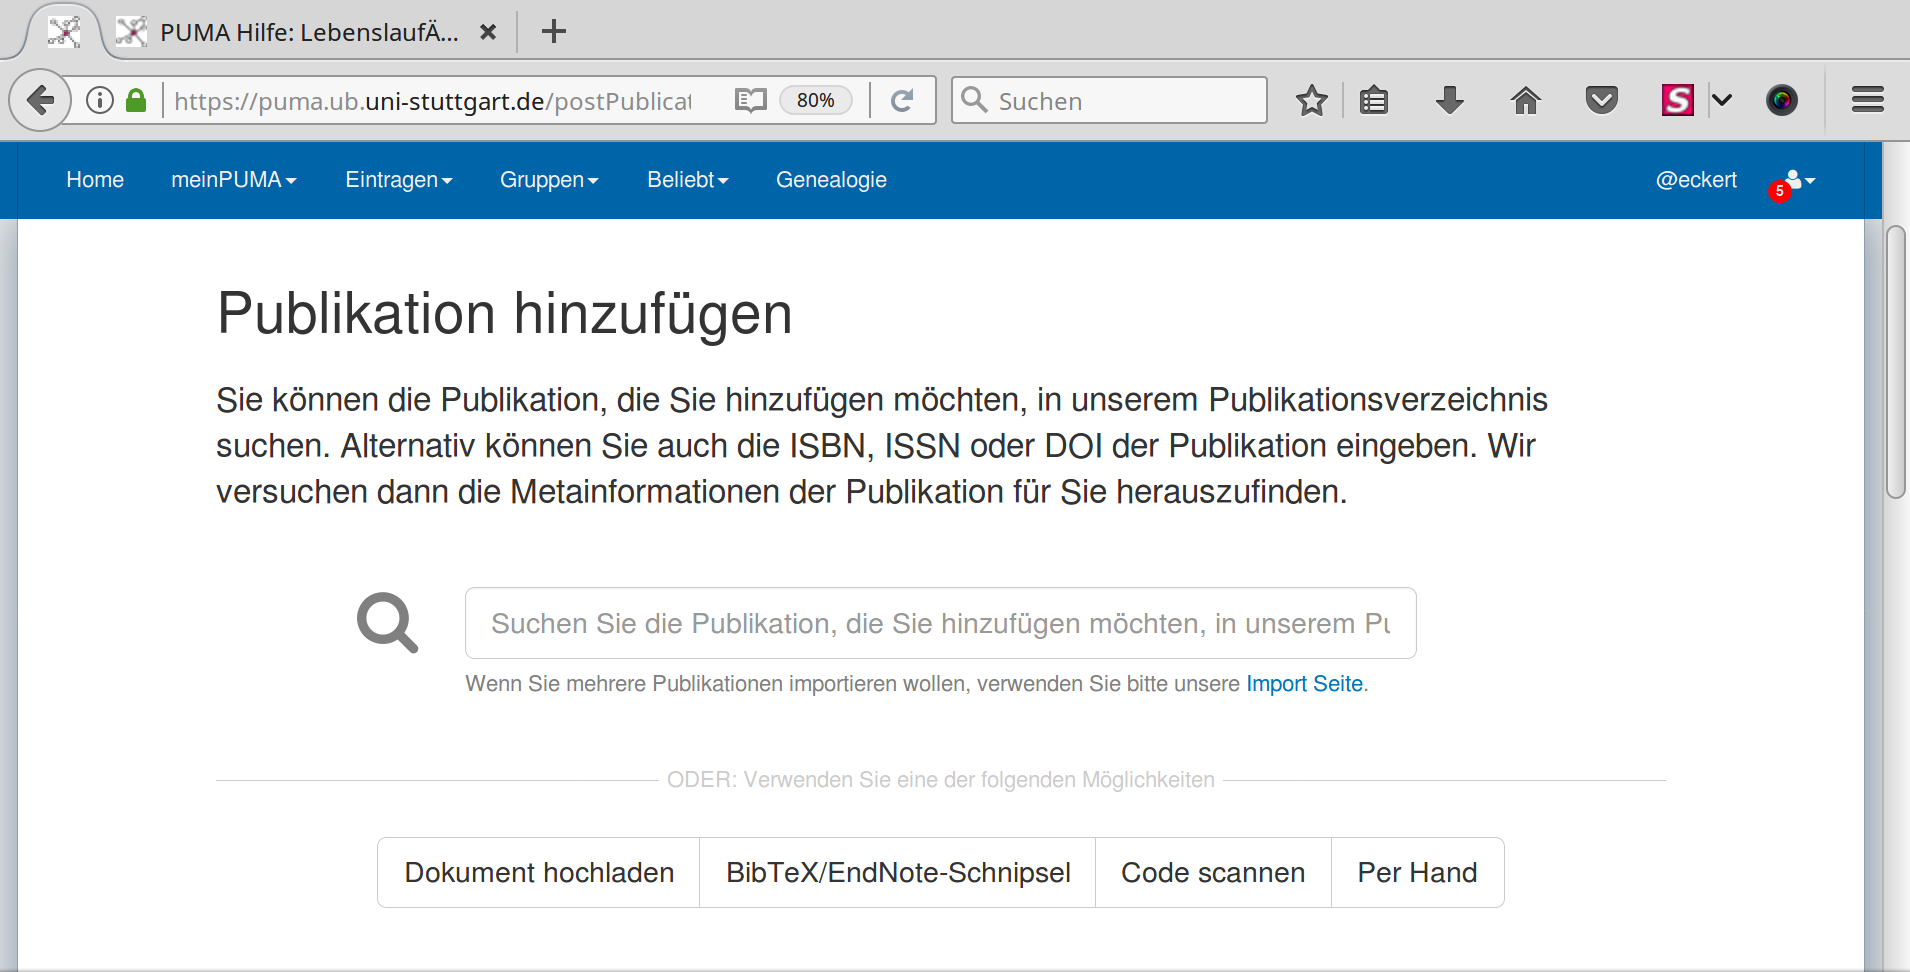
\includegraphics[width=11cm]{Bilder/Kapitel5/Eintragsmoeglichkeiten}}
 \caption{Eintragsmöglichkeiten}
 \label{fig:eintragungsmoeglichkeiten}
\end{figure}  
    \begin{itemize}
    	\item Dokument hochladen:\newline
        Voraussetzung ist, dass es sich um eine BibTex- oder EndNote-Datei handelt.
        \begin{enumerate}
            \item Klicken Sie auf \enquote{Datei hochladen}.
            \item Über den \enquote{Durchsuchen} Button haben Sie die Möglichkeit die gewünschte Datei auszuwählen.
            \item Der Dateiname, der ausgewählten Datei, erscheint hinter dem Durchsuchen-Button. Sie können anschließend die Sichtbarkeit des Eintrags festlegen. Durch das Klicken auf \enquote{Speichern} erhalten Sie die Detailansicht der Publikation und können diese nochmals überarbeiten und auf ihre Richtigkeit überprüfen.
            \item Klicken Sie anschließend nochmals auf \enquote{Speichern} um die Publikation in Ihre Sammlung einzutragen.
        \end{enumerate}
        \item BibTex\index{BibTex}/EndNote\index{EndNote}-Schnipsel:
        \newline
        Voraussetzung ist, dass Sie Ihre Literaturliste aus Ihrem bisherigen Literaturverwaltungsprogramm in die Zwischenablage exportieren.
        \begin{enumerate}
            \item Klicken Sie auf den Reiter \enquote{BibTex/EndNote-Schnipsel}.
            \item Fügen Sie den Text aus der Zwischenablage in das Textfeld \enquote{Auswahl} ein. Dies können Sie so erreichen, indem Sie auf das Textfeld Auswahl gehen und mit der rechte Maustaste das Menü öffnen und auf \enquote{Einfügen} klicken. Erscheint das Wort \enquote{Einfügen} grau, dann haben Sie keine Daten in die Zwischenablage exportiert und Sie müssen den Text erneut in die Zwischenablage einfügen.
            \item Klicken Sie auf \enquote{Weiter}.
            \item PUMA zeigt Ihnen nun eine Übersicht über alle Daten an. Überprüfen Sie diese auf ihre Richtigkeit.
            \item Klicken Sie \enquote{Speichern}.
        \end{enumerate}
        \item Code scannen\index{Code Scannen}: 
        \newline
        Voraussetzung ist, dass Sie über eine eingebaute Webcam verfügen oder eine externe Webcam anschließen, bevor Sie mit der Aufnahme beginnen können.
        \begin{enumerate}
            \item Klicken Sie auf den Reiter \enquote{Code scannen}. Es kann passieren, dass Ihr Webbrowser eine Warnmeldung anzeigt, dass die Webseite (PUMA) versucht auf Ihre Webcam zuzugreifen. Falls dies der Fall sein sollte, erlauben Sie den Zugriff.
            \item Das Bild der Webcam erscheint auf Ihrem Bildschirm. Halten Sie den Strichcode ruhig und gut sichtbar vor Ihre Webcam. Sobald PUMA den ISBN-Strichcode erkennt, ertönt ein Kamerageräusch.
            \item Wenn der Strichcode erkannt wurde, werden die Daten automatisch angezeigt. Überprüfen Sie diese auf ihre Richtigkeit und klicken Sie anschließend auf \enquote{Speichern}.
        \end{enumerate}
\begin{figure}[h!]
 \centering
 \fbox{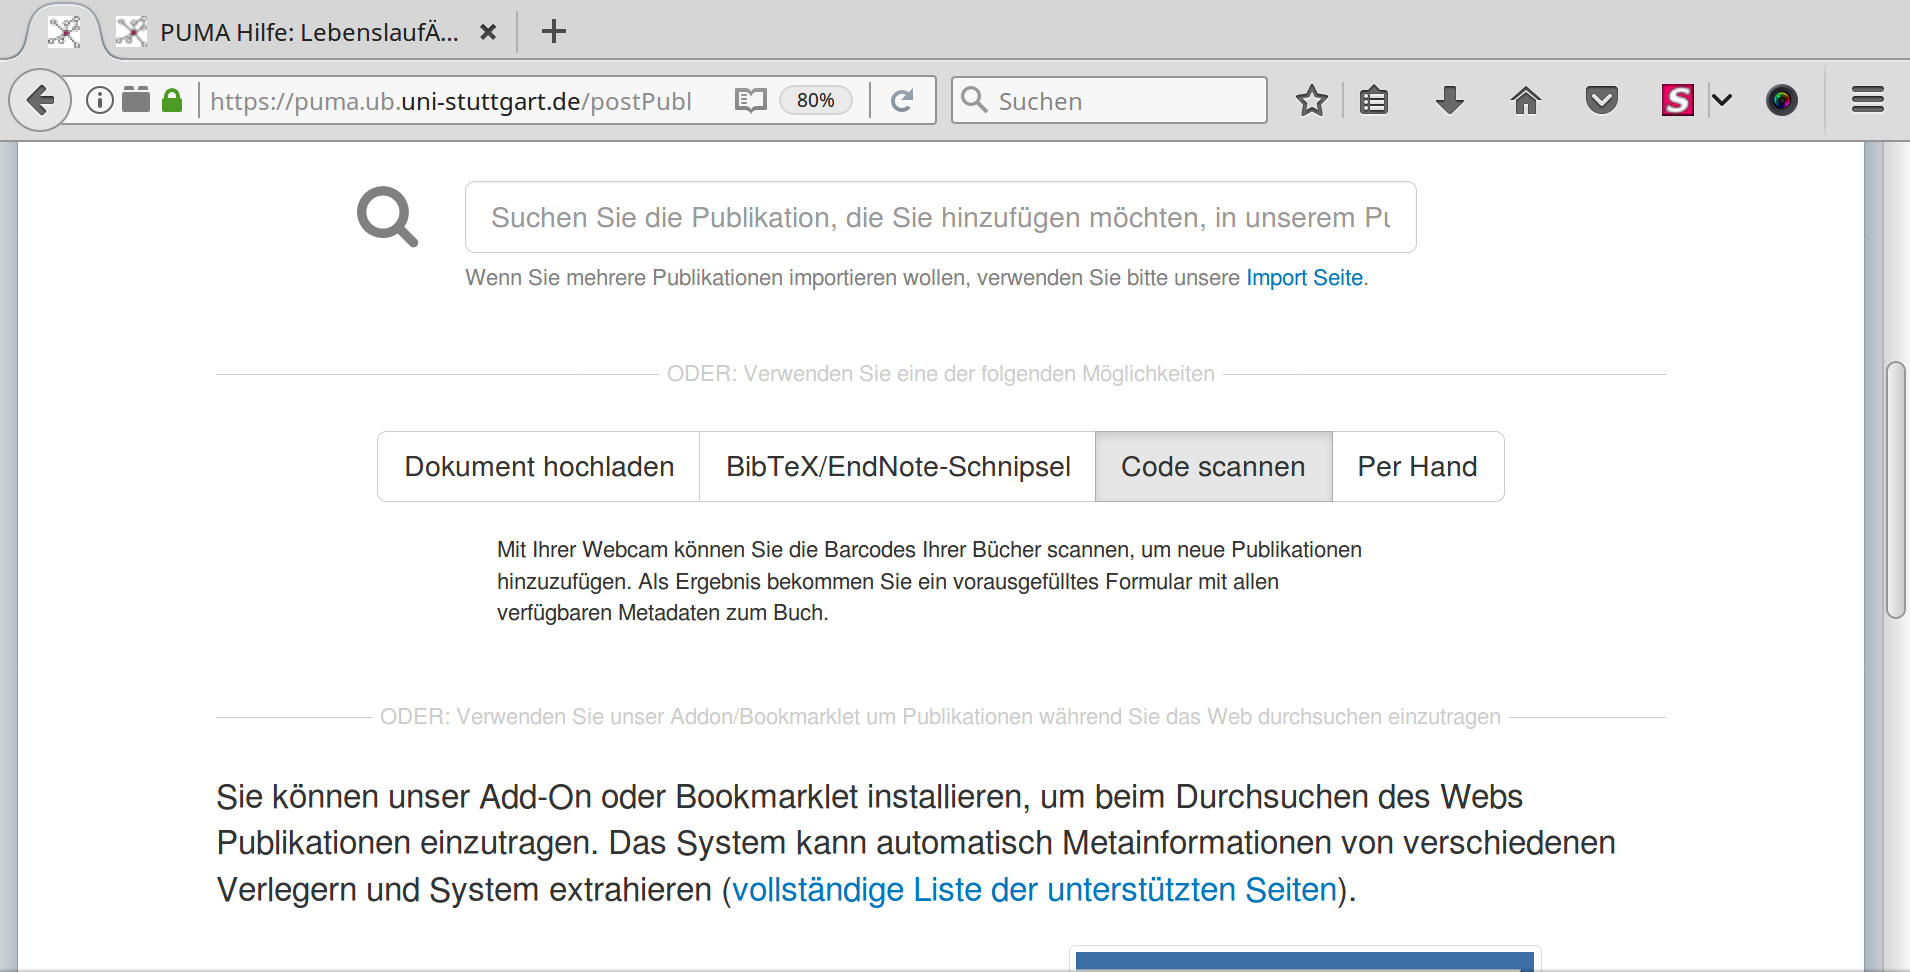
\includegraphics[width=11cm]{Bilder/Kapitel5/Code_scannen}}
 \caption{Code scannen}
 \label{fig:codeScannen}
\end{figure}  
        \item Per Hand:
        \begin{enumerate}
            \item Klicken Sie auf den Reiter \enquote{Per Hand}.
            \item Geben Sie alle geforderten Daten in die entsprechenden Felder ein und klicken Sie anschließend auf \enquote{Weiter}. 
            \item Im nächsten Schritt können Sie weiterführende Informationen angeben. Sie können aber auch gleich auf \enquote{Speichern} klicken, um die Publikation einzutragen.
        \end{enumerate}        
    \end{itemize}
\end{enumerate}
\section{Lesezeichen} % 2Screenshots: Anfang+Möglichkeiten
\label{sec:lesezeichen}
Grundlagen:
\newline
Lesezeichen\index{Lesezeichen} (engl. Bookmark) ermöglichen es, das Internet wie ein Buch zu verwenden. Mit einem Lesezeichen merken Sie sich die genaue Adresse eines Internet-Dokuments. PUMA gibt Ihnen die Möglichkeit Lesezeichen zentral zu speichern, zu verwalten und auf sie zuzugreifen. 
\newline
\newline
Lesezeichen hinzufügen\index{Lesezeichen!hinzufügen}: 
\begin{figure}[h!]
 \centering
 \fbox{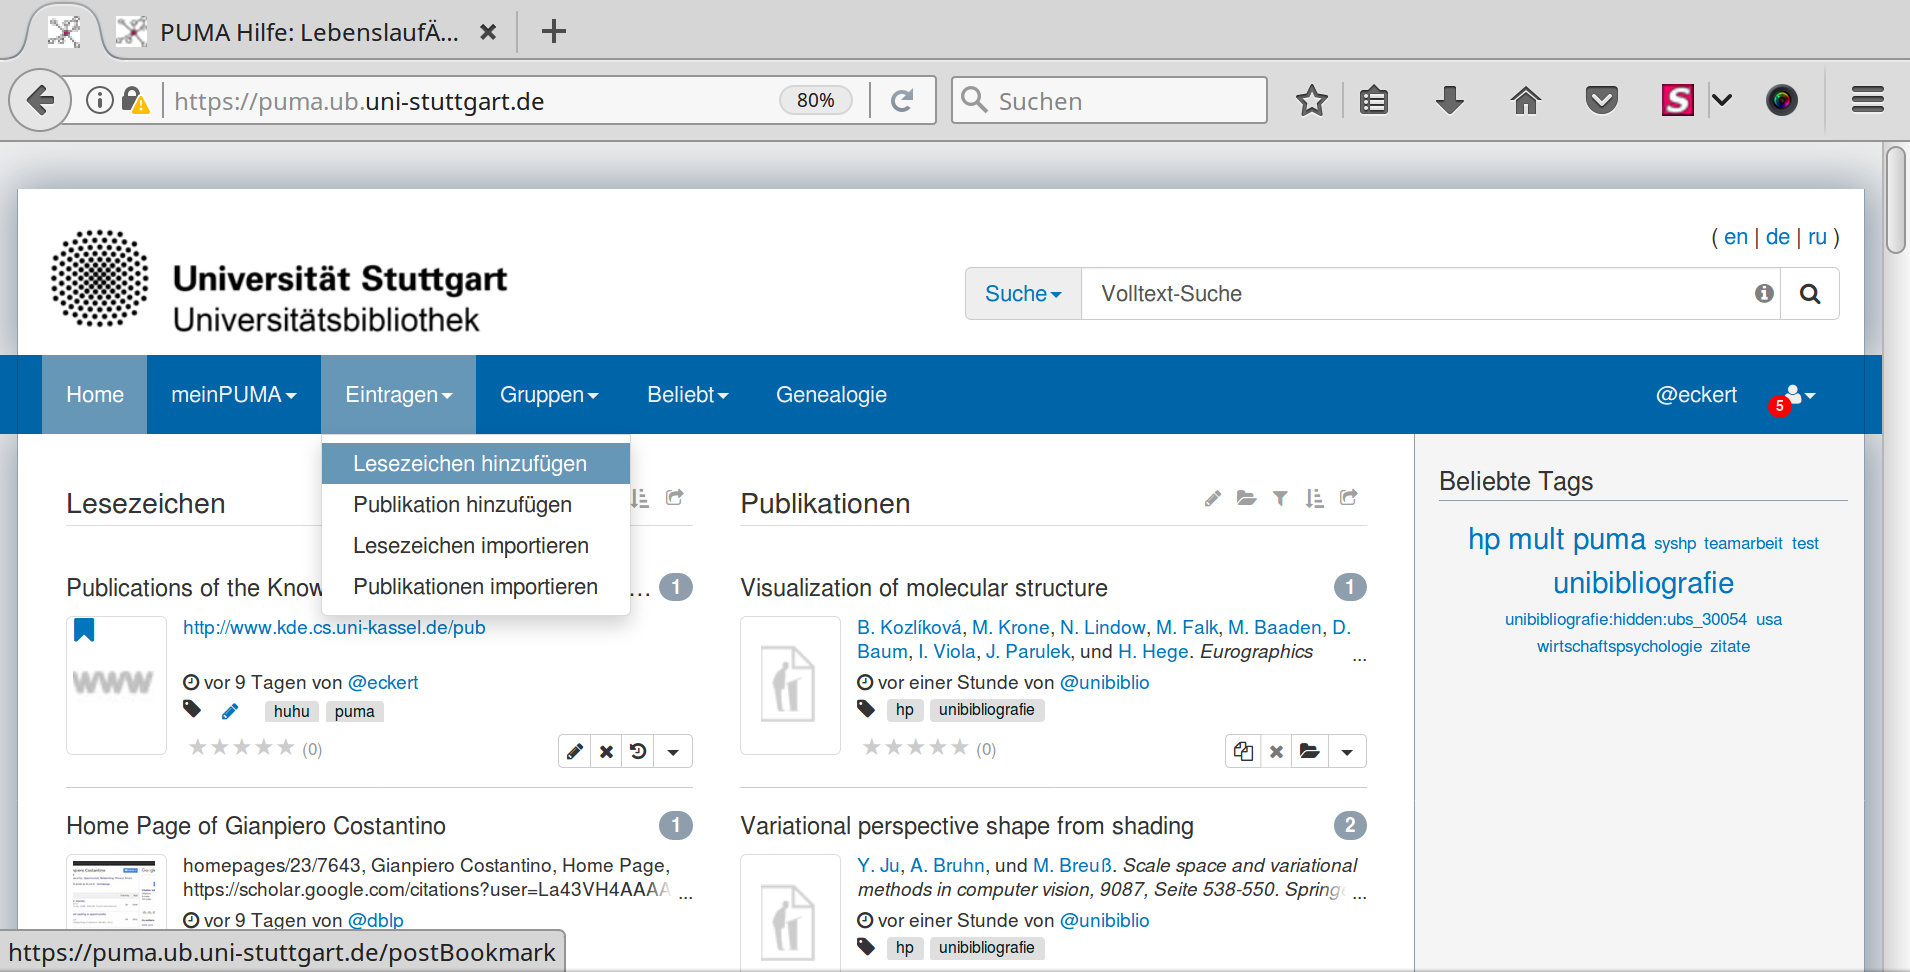
\includegraphics[width=11cm]{Bilder/Kapitel5/Lesezeichen_hinzufuegen}}
 \caption{Lesezeichen hinzufügen}
 \label{fig:lesezeichenHinzufuegen}
\end{figure} 
\begin{enumerate}
    \item Klicken Sie auf den Menüpunkt \enquote{Eintragen}\index{Lesezeichen!eintragen} im Hauptmenü. Ein Untermenü klappt auf.
    \item Klicken Sie im Untermenü auf \enquote{Lesezeichen hinzufügen}.
    \item Tragen Sie in das Feld \enquote{URL} die Adresse (URL) der Webseite ein, die Sie als Lesezeichen hinzufügen möchten. Anschließend klicken Sie auf \enquote{Weiter}. 
    \item Im Folgenden werden Sie aufgefordert einige Zusatzdaten einzugeben:
    \begin{itemize}
        \item URL: Wird automatisch aus dem Schritt davor übernommen.
        \item Titel: Tragen Sie den Titel der Seite ein. 
        \item Beschreibung/~Kommentar: Hier können Sie eigene Kommentare zum Lesezeichen hinterlegen. 
			%\begin{wrapfigure}{r}{5cm}
			\begin{mdframed}[style=tipp]\texttt{In diesem Feld können Sie z. B. auch ein kleines Abstract hinterlegen.} 
			\end{mdframed}
			%\end{wrapfigure}
        \item Tags: Tags\index{Tags} (dt. Schlagwörter) ermöglichen ein übersichtliches Organisieren und Strukturieren der Lesezeichen. Sie können so viele Tags verwenden, wie Sie wollen. Die einzelnen Tags werden durch Leerzeichen von einander getrennt. \newline 
        	%\begin{wrapfigure}{r}{5cm}
        	\begin{mdframed}[style=tipp]
	\texttt{Wenn Sie einen Tag verwenden möchten, der aus mehreren Worten besteht (z.~B. Fachbereich Architektur) dann verwenden Sie PascalCase, z.~B. FachbereichArchitektur.} 
			\end{mdframed}
			%\end{wrapfigure}
        \item Sichtbarkeit: Legen Sie fest, wer Ihr Lesezeichen sehen darf. Sie können wählen zwischen öffentlich\index{Sichtbarkeit!öffentlich} (alle Nutzer), privat\index{Sichtbarkeit!privat} (nur Sie selbst) oder andere\index{Sichtbarkeit! andere} (Freunde oder eine Gruppe). Außerdem können Sie bei \enquote{Interessant für} eine spezielle Gruppe auf Ihr Lesezeichen aufmerksam machen.  
    \end{itemize}
    \item Klicken Sie abschließend auf \enquote{Speichern} um das Lesezeichen einzutragen. Das Lesezeichen ist nun gespeichert. Bitte beachten Sie, dass ein neues Lesezeichen bei der Suchanfrage ein bisschen Zeit benötigt (1 Sekunde bis weniger als eine Minute). 
\end{enumerate}
\underline{Wichtig bei der Recherche und Archivierung von Lesezeichen:}
\begin{itemize}
    \item Puma speichern nicht das eigentliche Dokument, sondern nur die Adresse des Internet-Dokuments. Es kann somit passieren, dass ein Dokument zu einem späteren Zeitpunkt nicht mehr abrufbar ist, da z.B. sich die Adresse geändert hat oder es gelöscht wurde.  Aus diesem Grund ist es nützlich, dass Sie sich ein Sicherheitskopie des Dokuments anlegen und diese auf Ihrem Computer speichern.
    \item Neben den oben genannten Punkten bitten wir Sie auch darum zu bedenken, dass ein Internet-Dokument jederzeit geändert werden kann. Aus diesem Grund empfiehlt sich hier ebenfalls eine Sicherungskopie. 
    \item Zudem sollten Sie beachten, dass in der Literaturangabe zu einem Internet-Dokument IMMER das Datum und die Uhrzeit des letzten Abrufs mit angegeben werden muss. Dies entspricht den allgemeinen Richtlinien wissenschaftlichen Arbeitens. Diese Angaben können Sie in das Feld Beschreibung/~Kommentar eintragen.
    \item PUMA unterstützt die RFC 7089\footnote{\url{http://tools.ietf.org/html/rfc7089}} Spezifikation\index{RFC 7089 Spezifikation}. Damit wird es möglich, Lesezeichen so zu betrachten, wie sie in PUMA gespeichert wurden, selbst wenn sich die Seite in der Zwischenzeit geändert hat. Um diese Funktion zu nutzen, müssen Sie das Memento-Plugin in ihrem Browser installieren. Das Plugin existiert für Mozilla Firefox\footnote{\url{https://addons.mozilla.org/de/firefox/addon/mementofox/}} und Google Chrome\footnote{\url{https://chrome.google.com/webstore/detail/memento-time-travel/jgbfpjledahoajcppakbgilmojkaghgm?hl=en&gl=US}}. 
\end{itemize}
\section{Versionierung der Publikationen und Lesezeichen}
\label{sec:versionierung}
Publikationen und Lesezeichen können jederzeit eingetragen und bearbeitet werden. Um sich einen Überblick über die vorgenommen Änderungen zu verschaffen, bietet PUMA eine Versionsgeschichte\index{Versionierung} zu jeder Publikation und jedem Lesezeichen an. Klicken Sie in Ihrer eigenen Sammlung auf den kleinen schwarzen Pfeil neben einer beliebigen Publikation. Es öffnet sich ein Dropdown-Menü, in dem Sie \enquote{Verlauf dieser Publikation} auswählen. Ihnen wird sofort die Versionsgeschichte der jeweiligen Publikation/~Lesezeichen angezeigt und Sie können jede Ihrer Änderungen nachverfolgen. 
\begin{figure}[h!]
 \centering
 \fbox{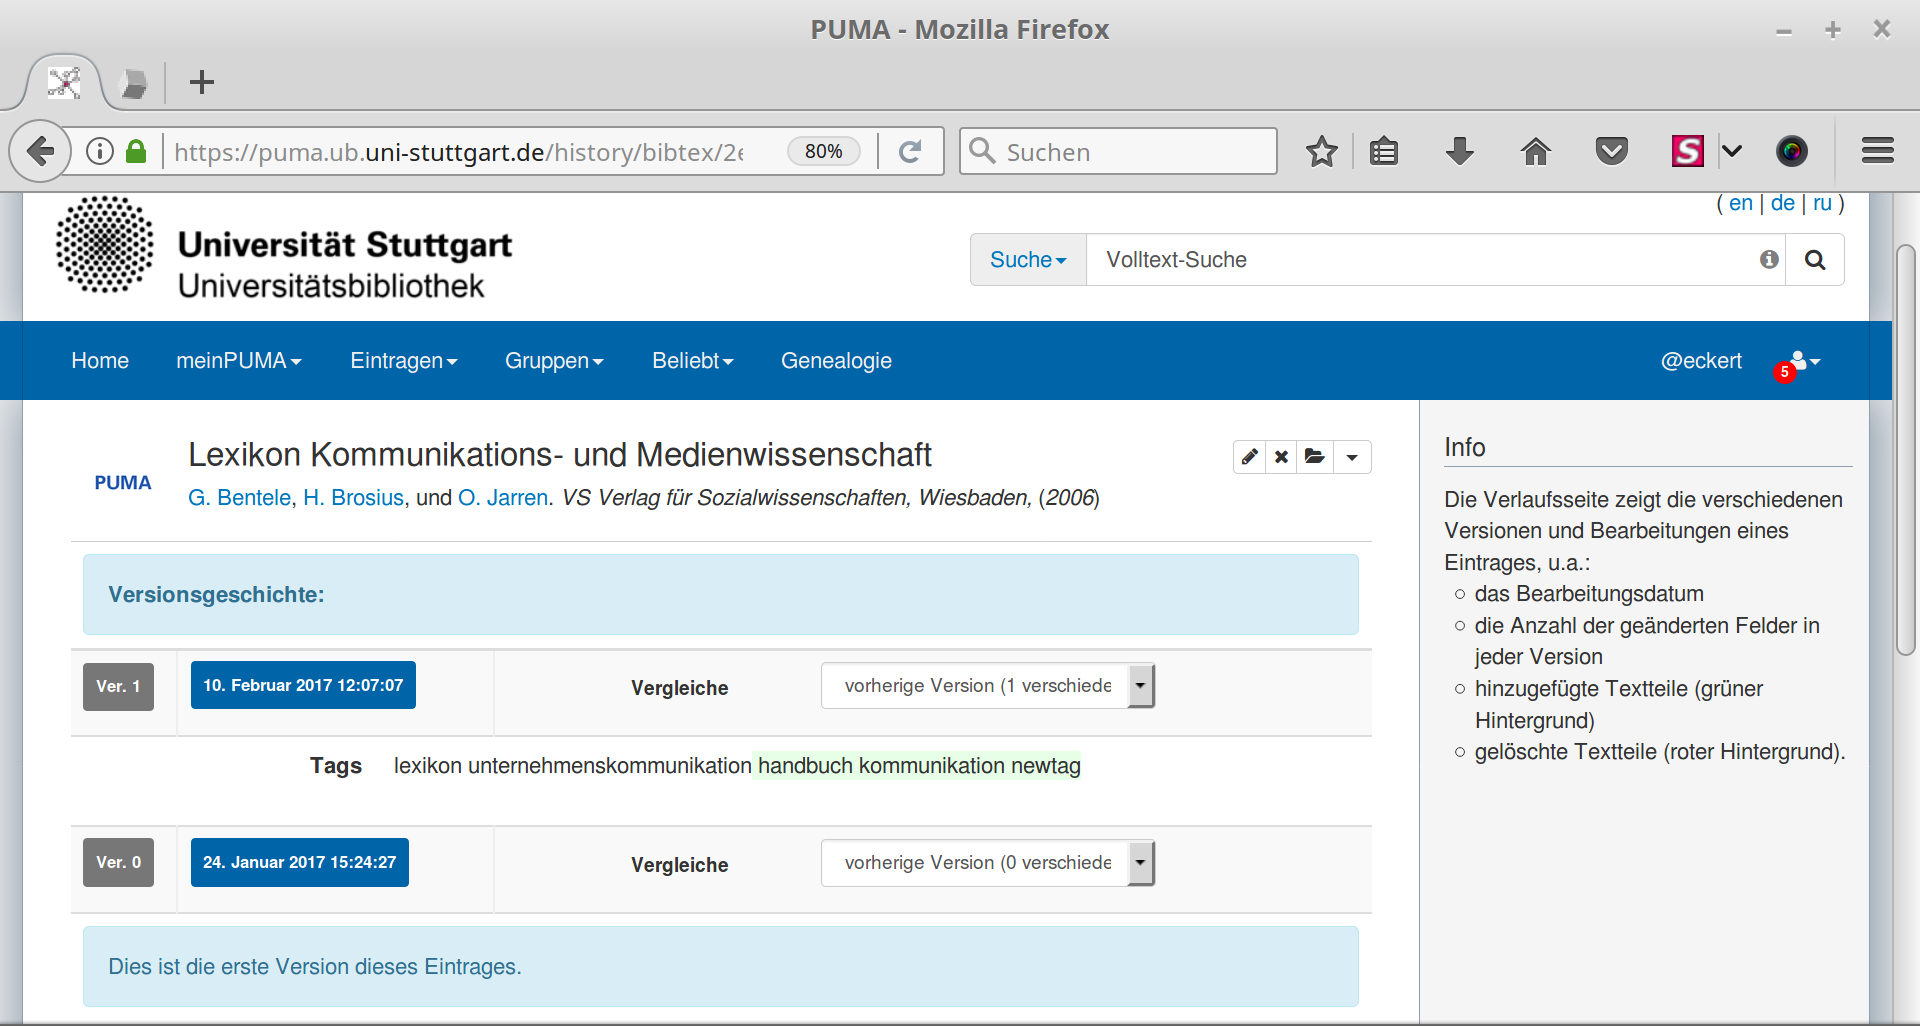
\includegraphics[width=9cm]{Bilder/Kapitel5/Versionsgeschichte}}
 \caption{Die Versionsgeschichte}
 \label{fig:versionsgeschichte}
\end{figure} 
\section{Lesezeichen importieren}
\label{sec:lesezeichenImportieren}
\subsection{Browser}
\label{subsec:browser}
PUMA ermöglicht es Ihnen HTML-Dateien in PUMA zu importieren. Hierfür exportieren Sie ihre Lesezeichen aus ihrem Browser als HTML-Datei und importieren diese anschließend. Je nach Browser unterscheidet sich das Exportieren der Lesezeichen.
\newline
\newline
\textbf{Chrome}%Screenshots hab ich schon
\newline Um ihre Lesezeichen in Chrome\index{Chrome} als HTML-Datei zu exportieren, klicken Sie im Menü oben rechts auf \enquote{Lesezeichen} und anschließend auf \enquote{Lesezeichen-Manager}. Es öffnet sich ein neues Fenster, in dem Sie auf \enquote{Organisieren} klicken und im Dropdown-Menü \enquote{Lesezeichen in HTML-Datei exportieren...} wählen. Speichern Sie die Datei ab und fahren mit Schritt 1 von HTML-Datei in PUMA importieren fort, um Ihre Lesezeichen endgültig nach PUMA zu importieren.  
\begin{figure}[h!]
 \centering
 \fbox{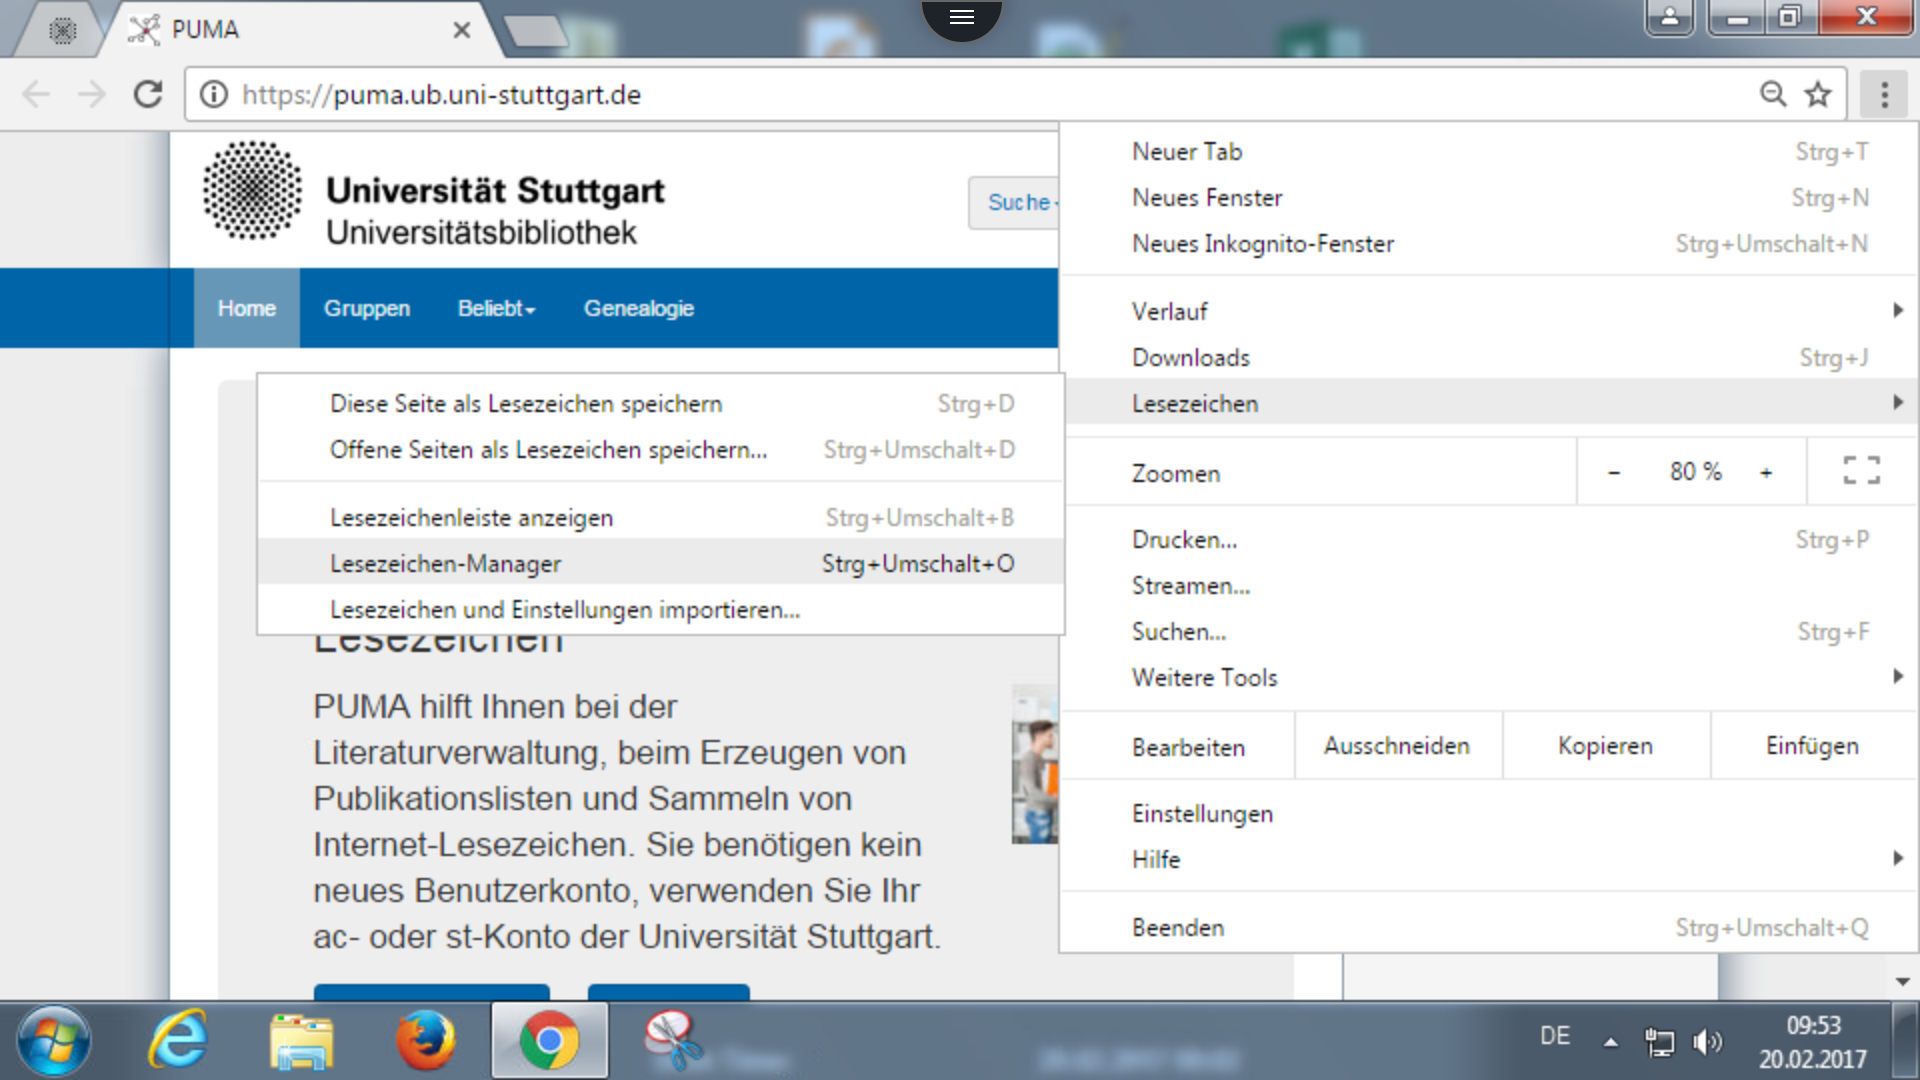
\includegraphics[width=11cm]{Bilder/Kapitel5/Lesezeichen-Manager_Chrome}}
 \caption{Der Lesezeichen-Manager}
 \label{fig:lesezeichenManager}
\end{figure}
\begin{figure}[ht]
 \centering
 \fbox{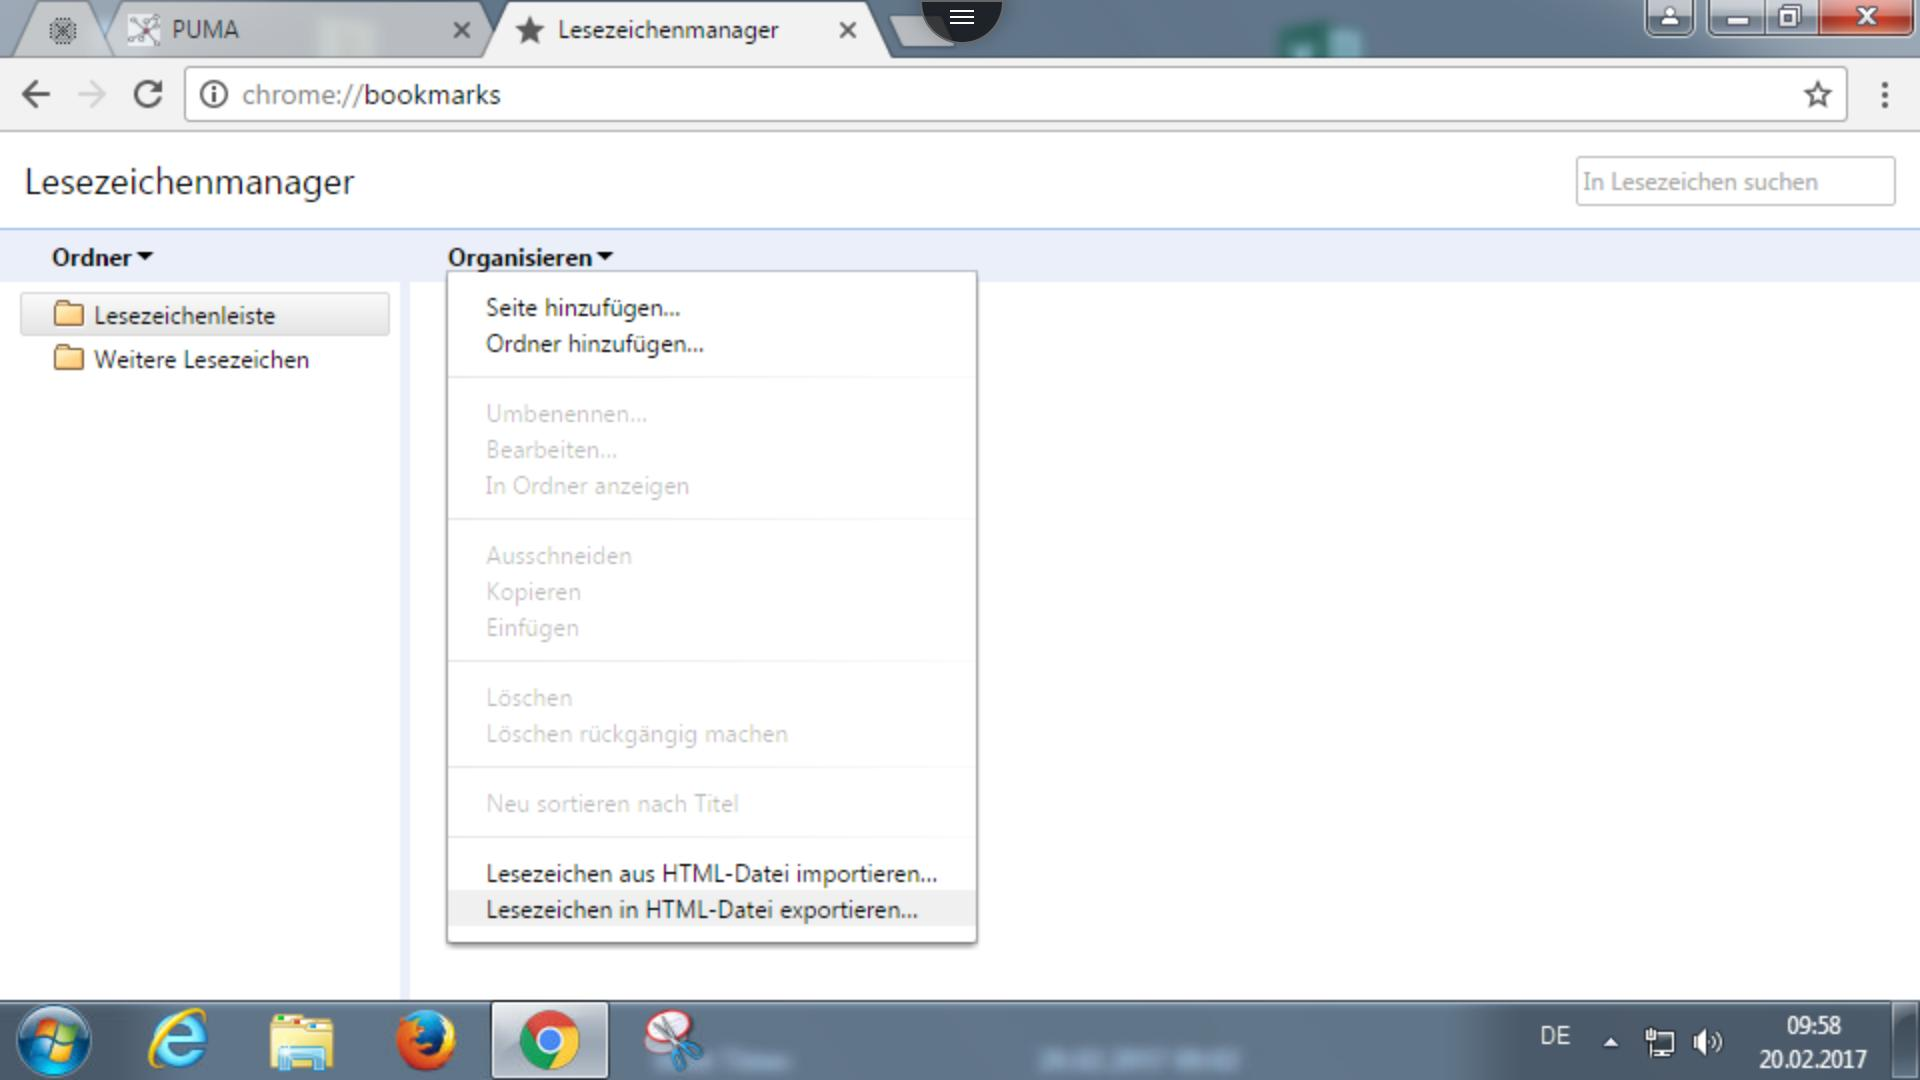
\includegraphics[width=9cm]{Bilder/Kapitel5/Lesezeichen_HTML_Chrome}}
 \caption{Lesezeichen in HTML-Datei exportieren}
 \label{fig:lesezeichenHtmlExportieren}
\end{figure}

\textbf{Firefox}
\newline Um Ihre Lesezeichen in Firefox\index{Firefox} als HTML-Datei zu exportieren, klicken Sie auf das Lesezeichensymbol rechts neben der Suchleiste. Wählen Sie im Dropdown-Menü \enquote{Lesezeichen verwalten} aus.

\begin{figure}[h!]
 \centering
 \fbox{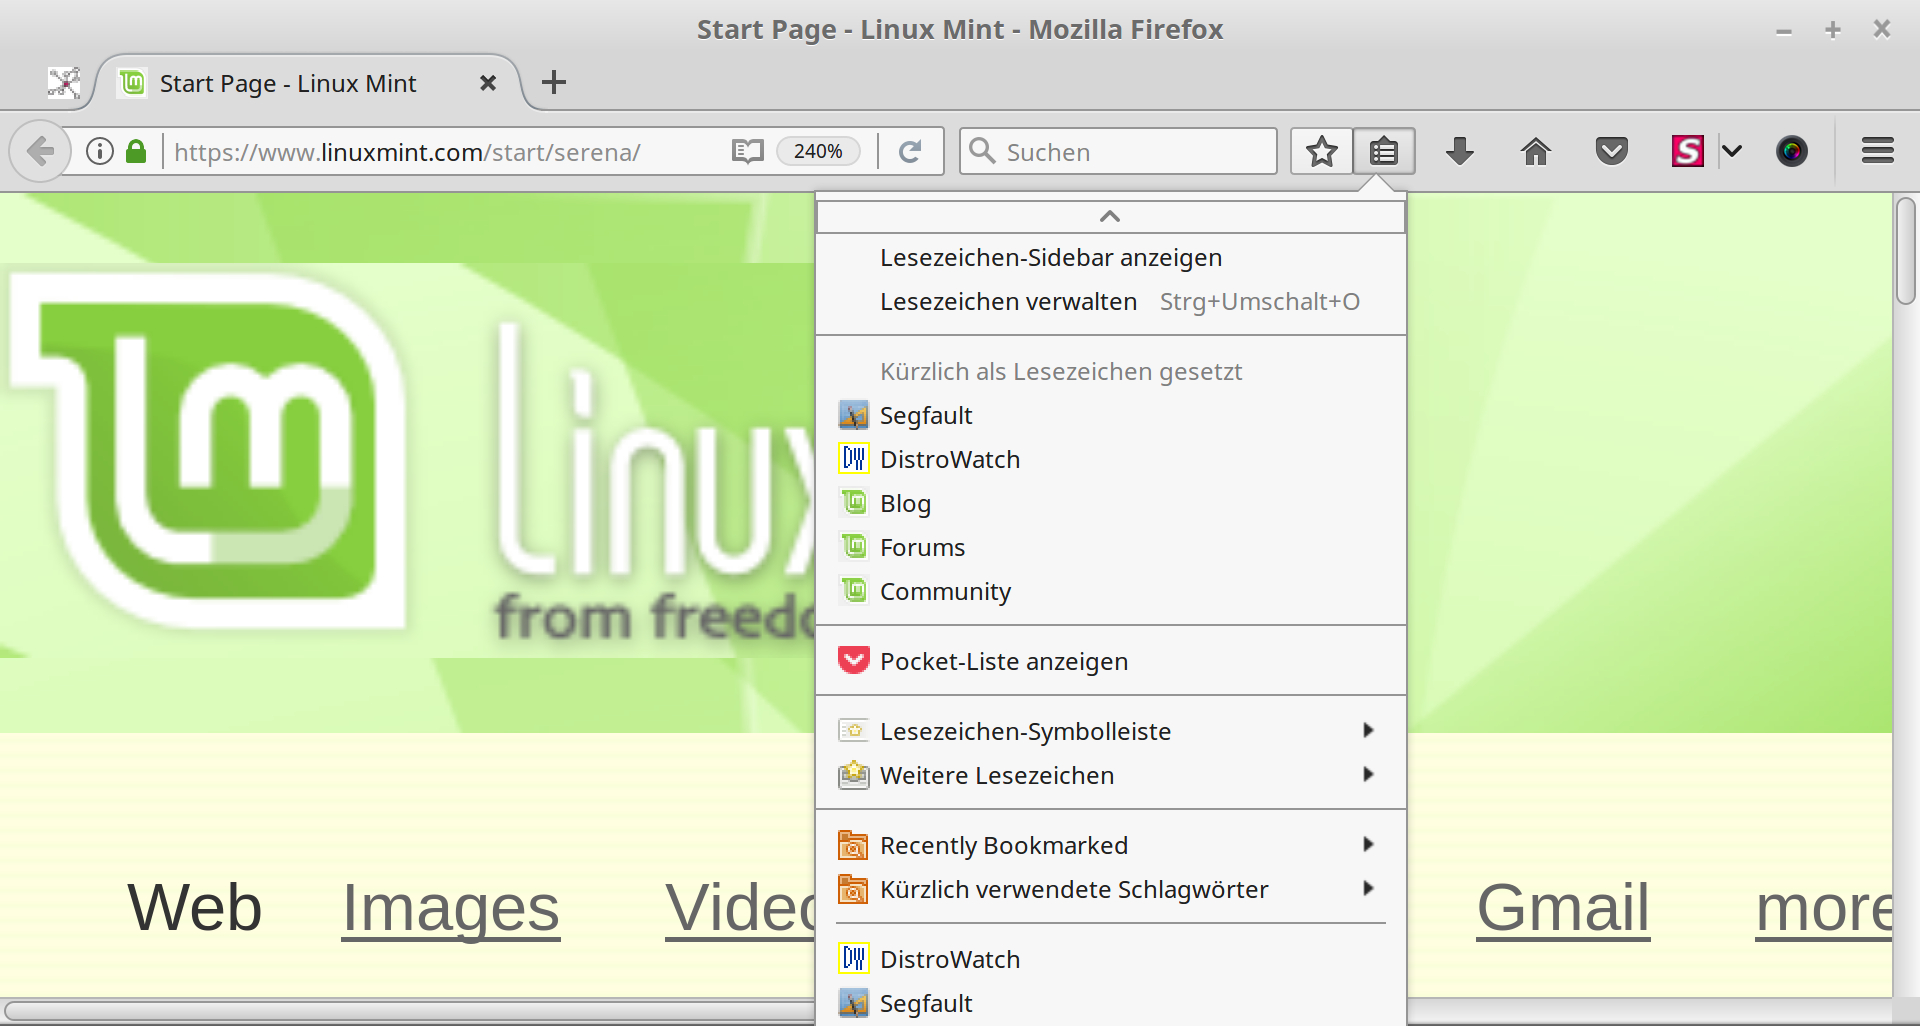
\includegraphics[width=11cm]{Bilder/Kapitel5/Firefox_Lesezeichen_verwalten}}
 \caption{Lesezeichen verwalten}
 \label{fig:lesezeichenVerwalten}
\end{figure}
Anschließend klicken Sie auf \enquote{Importieren und Sichern} und wählen \enquote{Lesezeichen nach HTML exportieren} aus. Speichern Sie die Datei ab und fahren mit Schritt 1 von HTML-Datei in PUMA importieren fort, um Ihre Lesezeichen endgültig nach PUMA zu importieren.  

\begin{figure}[h!]
 \centering
 \fbox{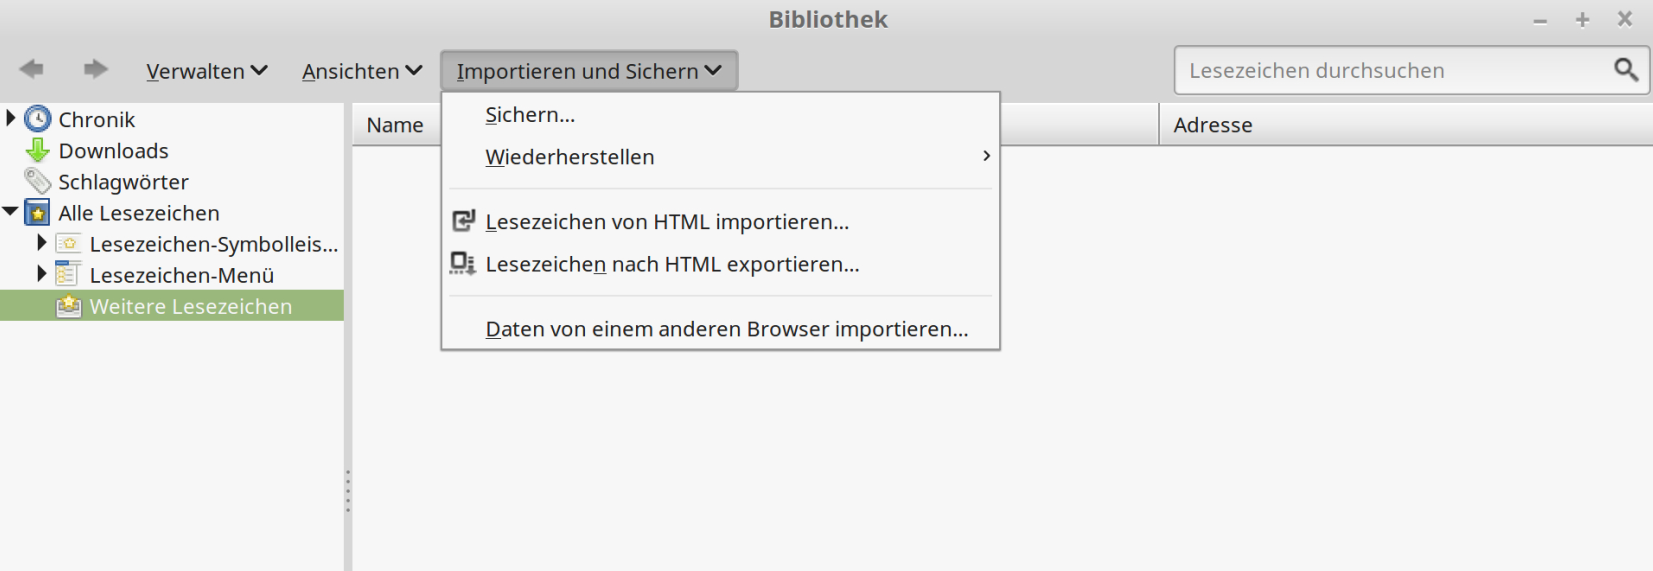
\includegraphics[width=11cm]{Bilder/Kapitel5/Firefox_Importieren_Speichern}}
 \caption{Importieren und Sichern}
 \label{fig:importierenSichern}
\end{figure}
\subsection{HTML-Datei\index{HTML-Datei} in PUMA importieren}
\label{subsec:htmlDateiImportieren}
\begin{enumerate}
    \item Klicken Sie auf \enquote{Eintragen} und wählen im Dropdown-Menü \enquote{Lesezeichen importieren} aus.
    \item Es öffnet sich eine neue Seite. In dem Bereich \enquote{Importieren Sie Ihre Lesezeichen aus Ihrem Browser} können Sie nun die entsprechende Datei hochladen. 
    \item Legen Sie die Sichtbarkeit der Lesezeichen fest und bestätigen Sie Ihren Import anschließend mit \enquote{Importieren}.
\end{enumerate}
\begin{figure}[h!]
 \centering
 \fbox{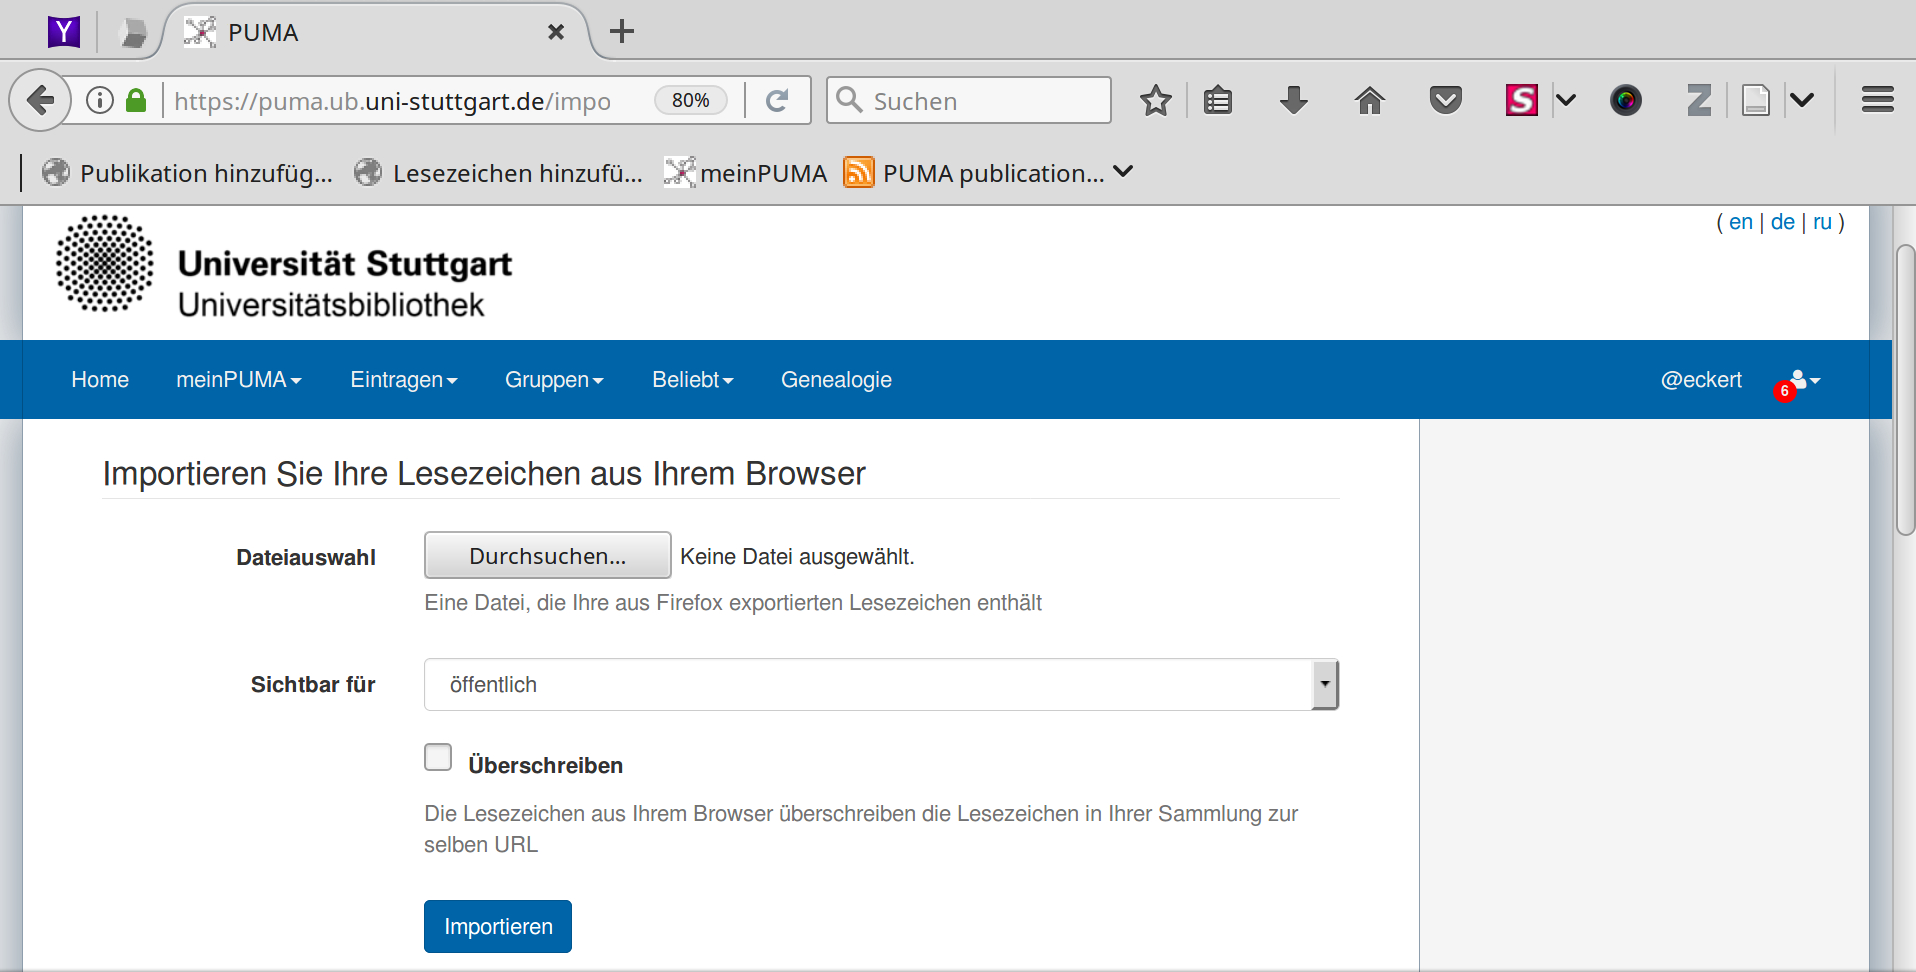
\includegraphics[width=11cm]{Bilder/Kapitel5/HTML-Datei_hochladen}}
 \caption{HTML-Datei hochladen}
 \label{fig:htmlDateiHochladen}
\end{figure}
\subsection{Delicious}
\label{subsec:delicious}
Sie möchten Ihre Lesezeichen von Delicious\index{Delicious} nach PUMA importieren. Klicken Sie auf \enquote{Eintragen} und wählen im Dropdown-Menü \enquote{Lesezeichen importieren} aus. Geben Sie unter dem Bereich \enquote{Importieren Sie Ihre Delicious Daten} Ihre Delicious-Nutzerdaten ein. \newline
Legen Sie im darauffolgenden Schritt fest, ob Ihre Delicious Lesezeichen bereits vorhandene Lesezeichen in Ihrer Sammlung mit der selben URL überschreiben sollen.\newline
Sie können im letzten Schritt festlegen, ob Sie Ihre Lesezeichen oder Tag-Bundles importieren möchten. Wenn Sie die Option \enquote{Lesezeichen} wählen, werden zusammen mit Ihren Lesezeichen die dazugehörigen Tags und Sichtbarkeitsdefinitionen mit übernommen.
\newline Klicken Sie abschließend auf \enquote{Importieren} um den Import endgültig durchzuführen.
\begin{figure}[h!]
 \centering
 \fbox{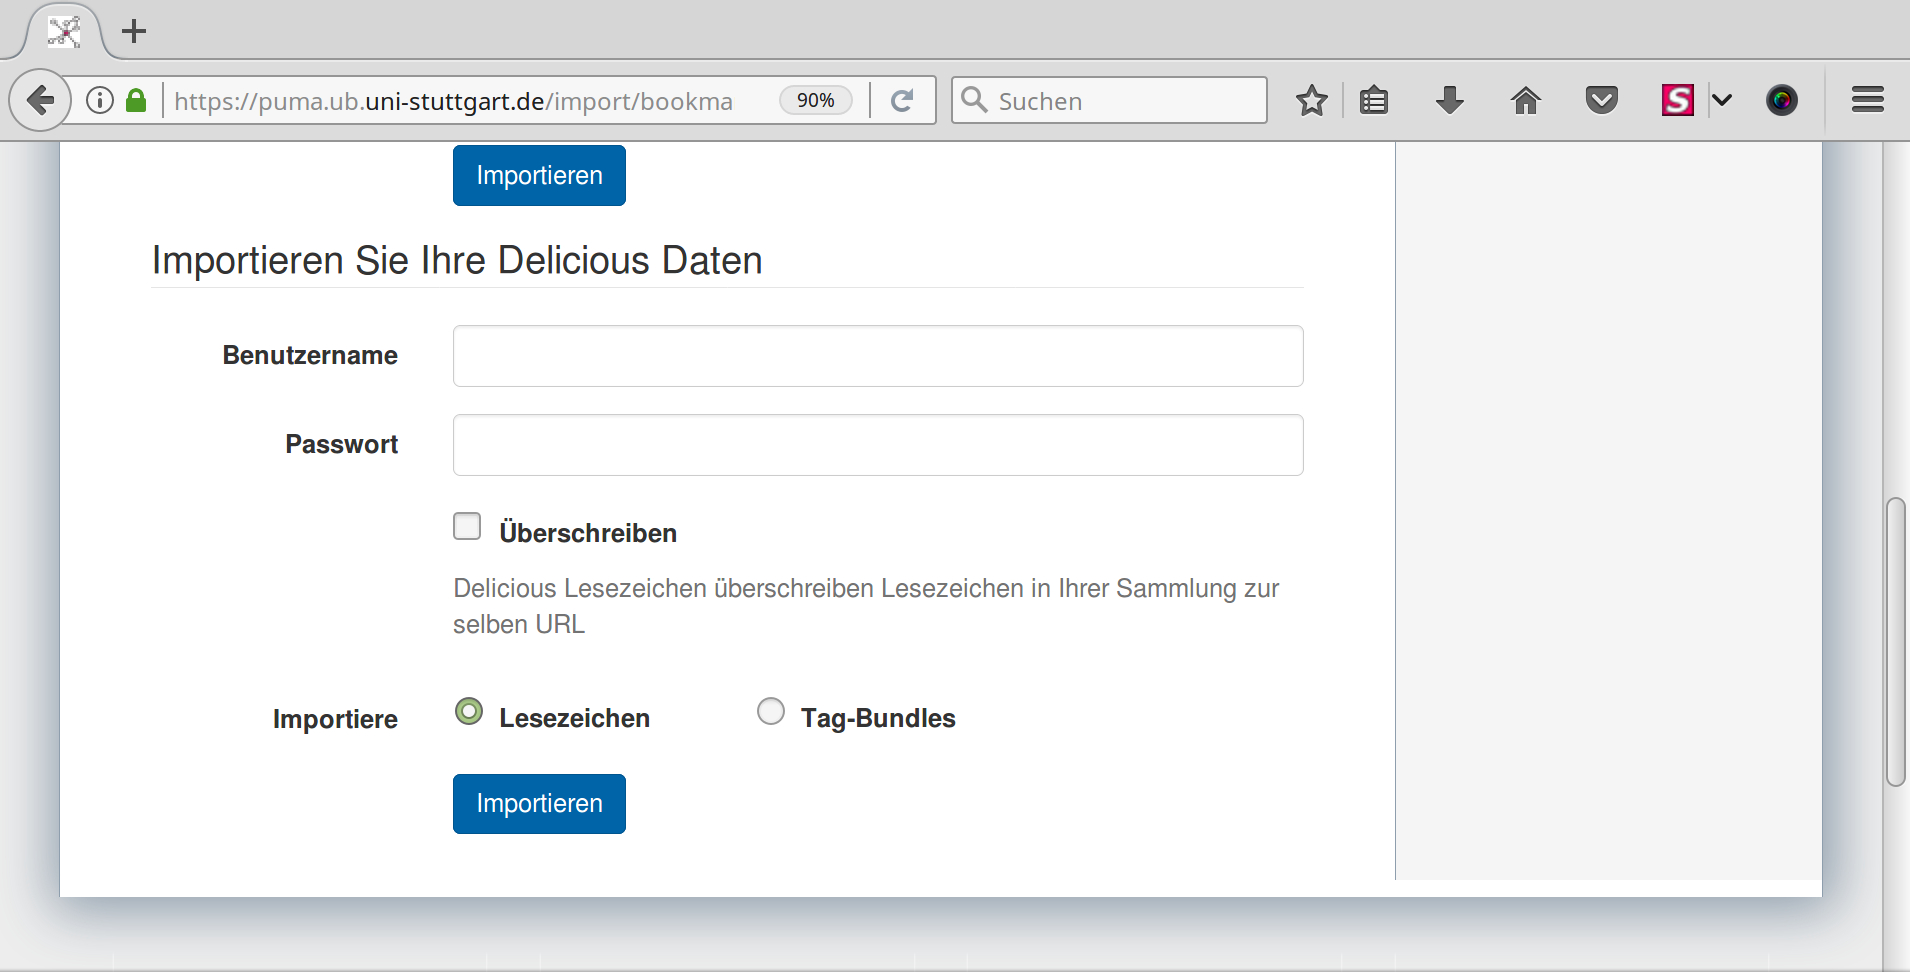
\includegraphics[width=11cm]{Bilder/Kapitel5/Delicious_Daten}}
 \caption{Delicious Daten}
 \label{fig:deliciousDaten}
\end{figure} 
\section{Publikationen importieren}
\label{sec:publikationenImportieren}
PUMA ermöglicht Ihnen bereits bestehende BibTeX- oder EndNote-Datei hochladen. Vergewissern Sie sich hierbei, dass Sie die korrekte Kodierung gewählt haben. Falls die Datei nur wenige Einträge enthält, können Sie diese auf der folgenden Seite bearbeiten. 
\begin{enumerate}
	\item Klicken Sie auf das Feld \enquote{Durchsuchen} und laden die entsprechende Datei hoch. 
	\item Wählen Sie die Sichtbarkeit aus.
	\item In den \enquote{Erweiterte Einstellungen} können Sie anschließend noch die Datei vor dem Import bearbeiten und festlegen, ob ein älterer Eintrag überschrieben werden soll, wenn der importierte Eintrag die gleiche Publikation referenziert wie ein bereits existierender Eintrag.
	\item Klicken Sie anschließend auf \enquote{Weiter}, um den Eintrag zu vervollständigen und zu speichern.
\end{enumerate}
\begin{figure}[h!]
 \centering
 \fbox{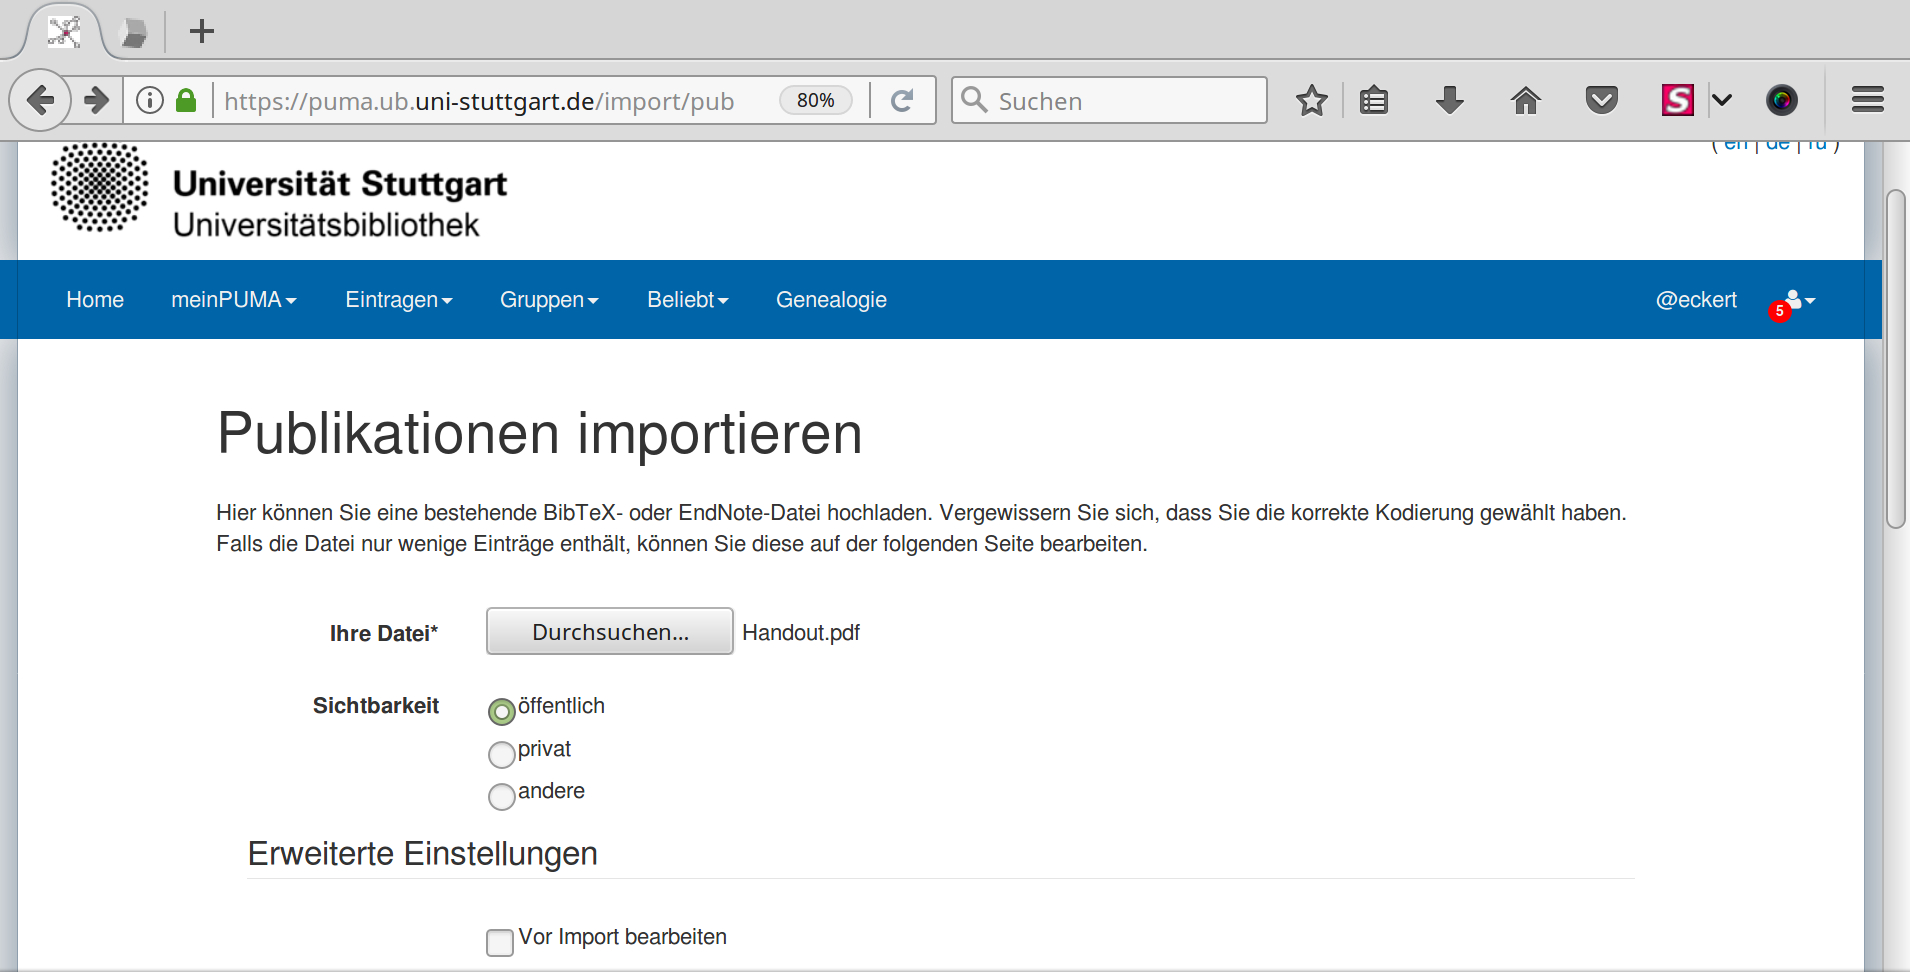
\includegraphics[width=11cm]{Bilder/Kapitel5/Publikationen_importieren}}
 \caption{Publikationen importieren}
 \label{fig:publikationenImportieren}
\end{figure}  



  
\section{Bookmarklet-Buttons für Ihre Lesezeichen-Leiste}\label{sec:button}
Die Bookmarklet-Buttons\index{Bookmarklet-Buttons} ermöglichen Ihnen ein schnelles Arbeiten mit PUMA, während Sie im Internet unterwegs sind. Sie vereinfachen Ihnen das Eintragen von Publikationen und Lesezeichen und gelangen mit dem PUMA-Home Bookmarklet-Button direkt zu PUMA. Ziehen Sie die Buttons\footnote{\url{https://puma.ub.uni-stuttgart.de/buttons}} einfach in Ihre Lesezeichen-Leiste und schon können Sie loslegen.
\begin{figure}[h!]
 \centering
 \fbox{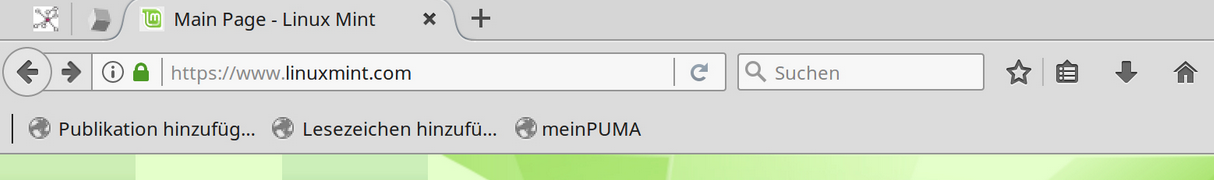
\includegraphics[width=11cm]{Bilder/Kapitel5/Bookmarklet-Buttons}}
 \caption{Bookmarklet-Buttons}
 \label{fig:bookmarkletButtons}
\end{figure} 
\section{PUMA-Browser-Add-ons\index{Add-ons}}\label{sec:addon}
Erweitern Sie Ihren Browser mit diesem Add-on um drei nützliche PUMA-Schaltflächen: Mit einem Klick zu PUMA, eine Publikation oder ein Lesezeichen speichern.\newline
\begin{enumerate}
\item Klicken Sie rechts oben im Firefox-Browser auf das Menü.
\begin{figure}[h!]
 \centering
 \fbox{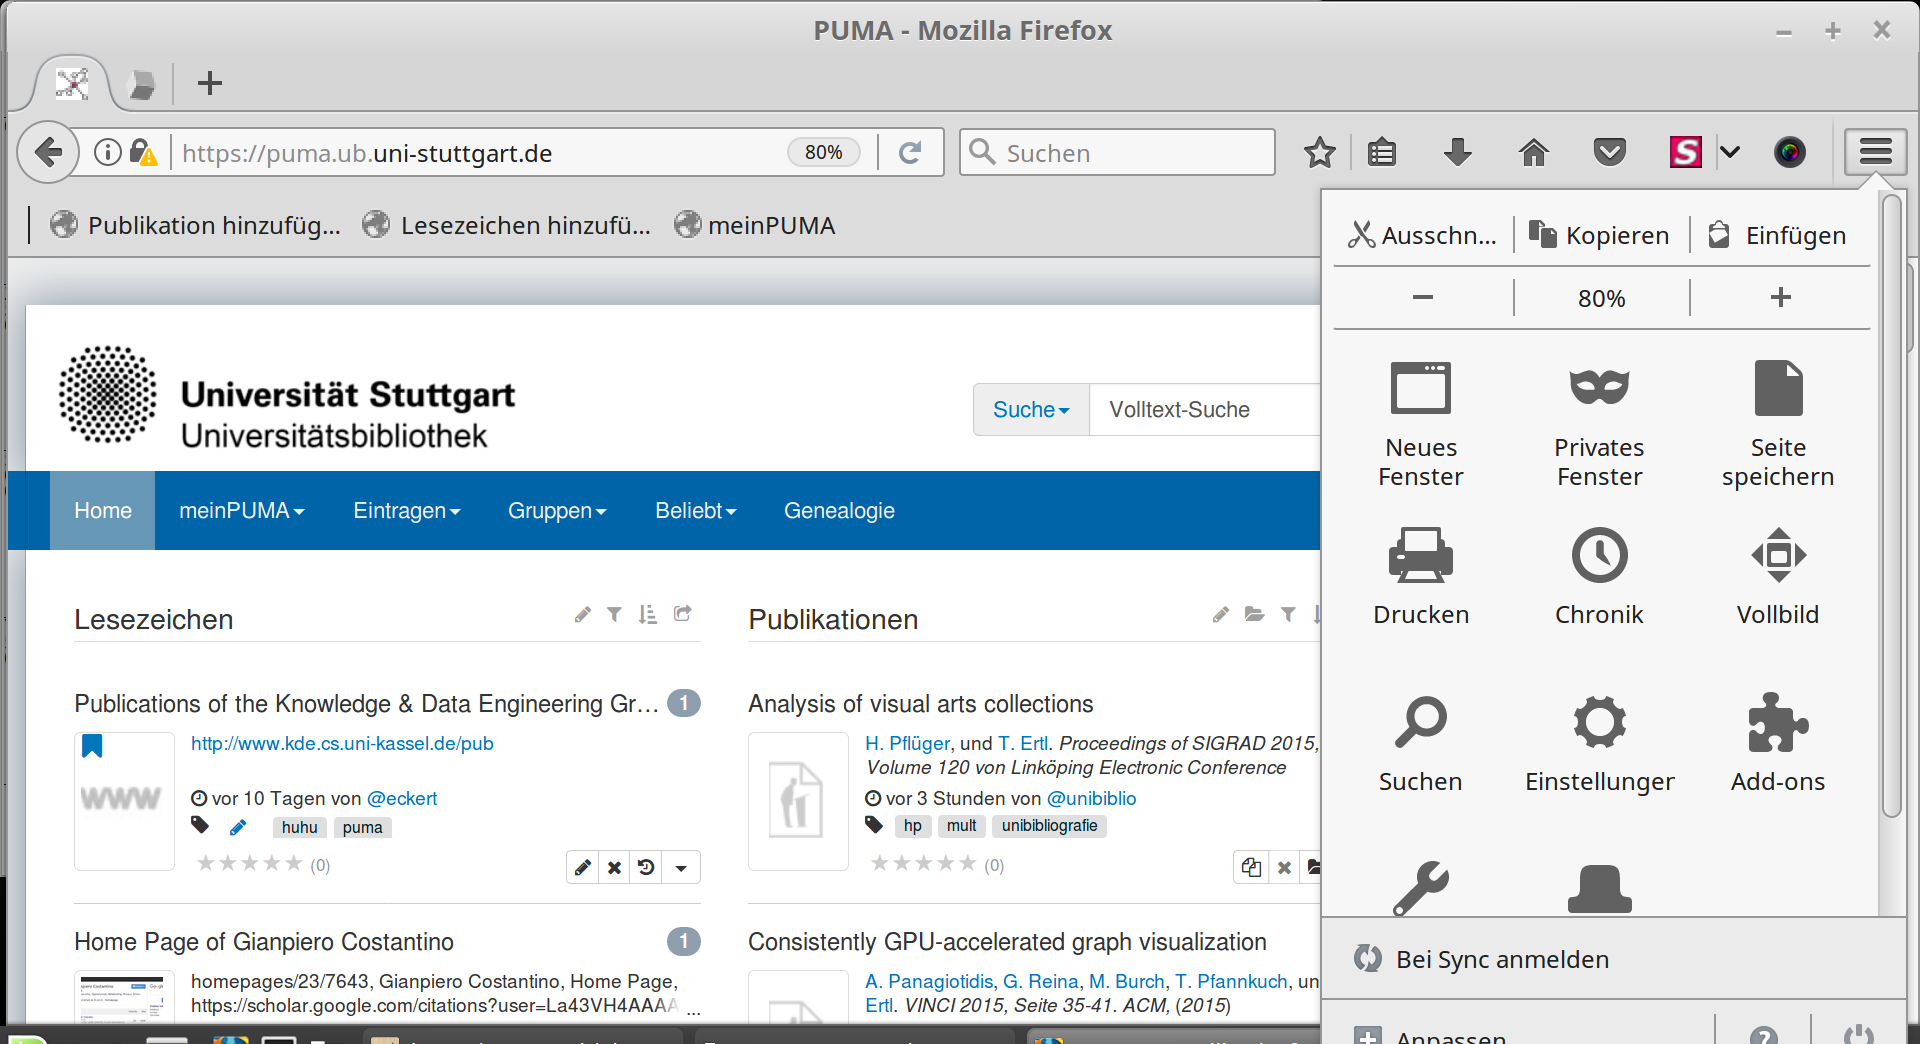
\includegraphics[width=11cm]{Bilder/Kapitel5/Menue_Firefox}}
 \caption{Firefox-Browser}
 \label{fig:firefoxBrowser}
\end{figure} 
\item Es öffnet sich das Menü, wählen Sie den Reiter \enquote{Add-ons} aus. 
\item Geben Sie in die Suchleiste oben rechts \enquote{puma} ein.
\item Es erscheint das Add-on \enquote{PUMA Buttons}. Installieren Sie die Buttons (Version 1.6.2).
\begin{figure}[h!]
 \centering
 \fbox{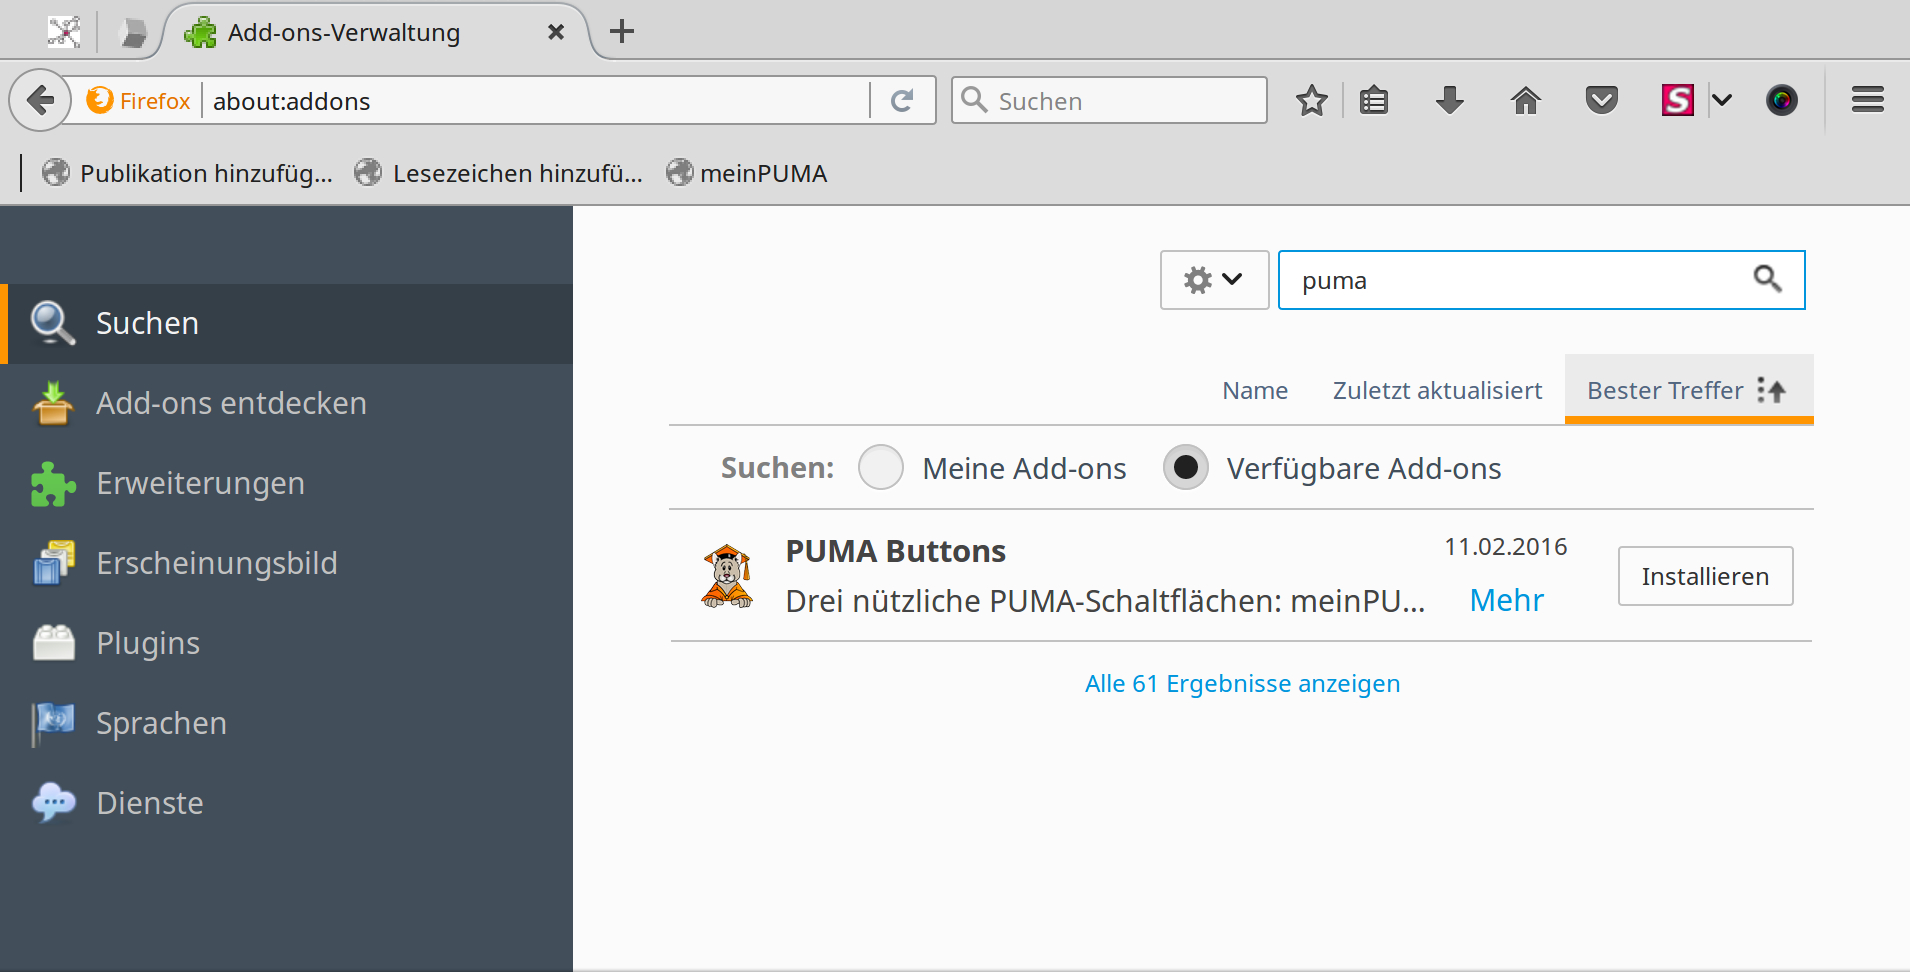
\includegraphics[width=11cm]{Bilder/Kapitel5/PUMA_Buttons}}
 \caption{Puma Buttons}
 \label{fig:pumaButtons}
\end{figure} 
\item Klicken Sie anschließend auf \enquote{mehr} und scrollen auf der Seite runter bis zum Abschnitt \enquote{Instanz wechseln}. 
\item Durch das Klicken auf \enquote{Instanz wechseln} öffnet sich eine Übersicht über alle verfügbaren PUMAs. Wählen Sie  \enquote{UB Stuttgart} aus und speichern Ihre Wahl.
\item Falls die Buttons nicht sofort in der Taskleiste neben dem Menüsymbol  erscheinen, schließen Sie Firefox. Beim erneuten Öffnen des Firefox-Browsers wurden die Buttons eingerichtet.
\end{enumerate}
\section{Ablage}
\label{sec:ablage}
Die Ablage\index{Ablage} ermöglicht es Ihnen eigene und fremde Publikationen vorzumerken. Sie können so in der Ablage aktuelle Literaturlisten zusammenstellen.
\newline
Publikationen in Ablage aufnehmen: %Screenshot
\begin{enumerate}
    \item Klicken Sie auf das Symbol \enquote{Diese Publikation zur Ablage hinzufügen}.
    \item Die Publikationen gelangen direkt in die Ablage. Zur Ablage gelangen Sie über das Personensymbol.
\end{enumerate}
\begin{figure}[h!]
 \centering
 \fbox{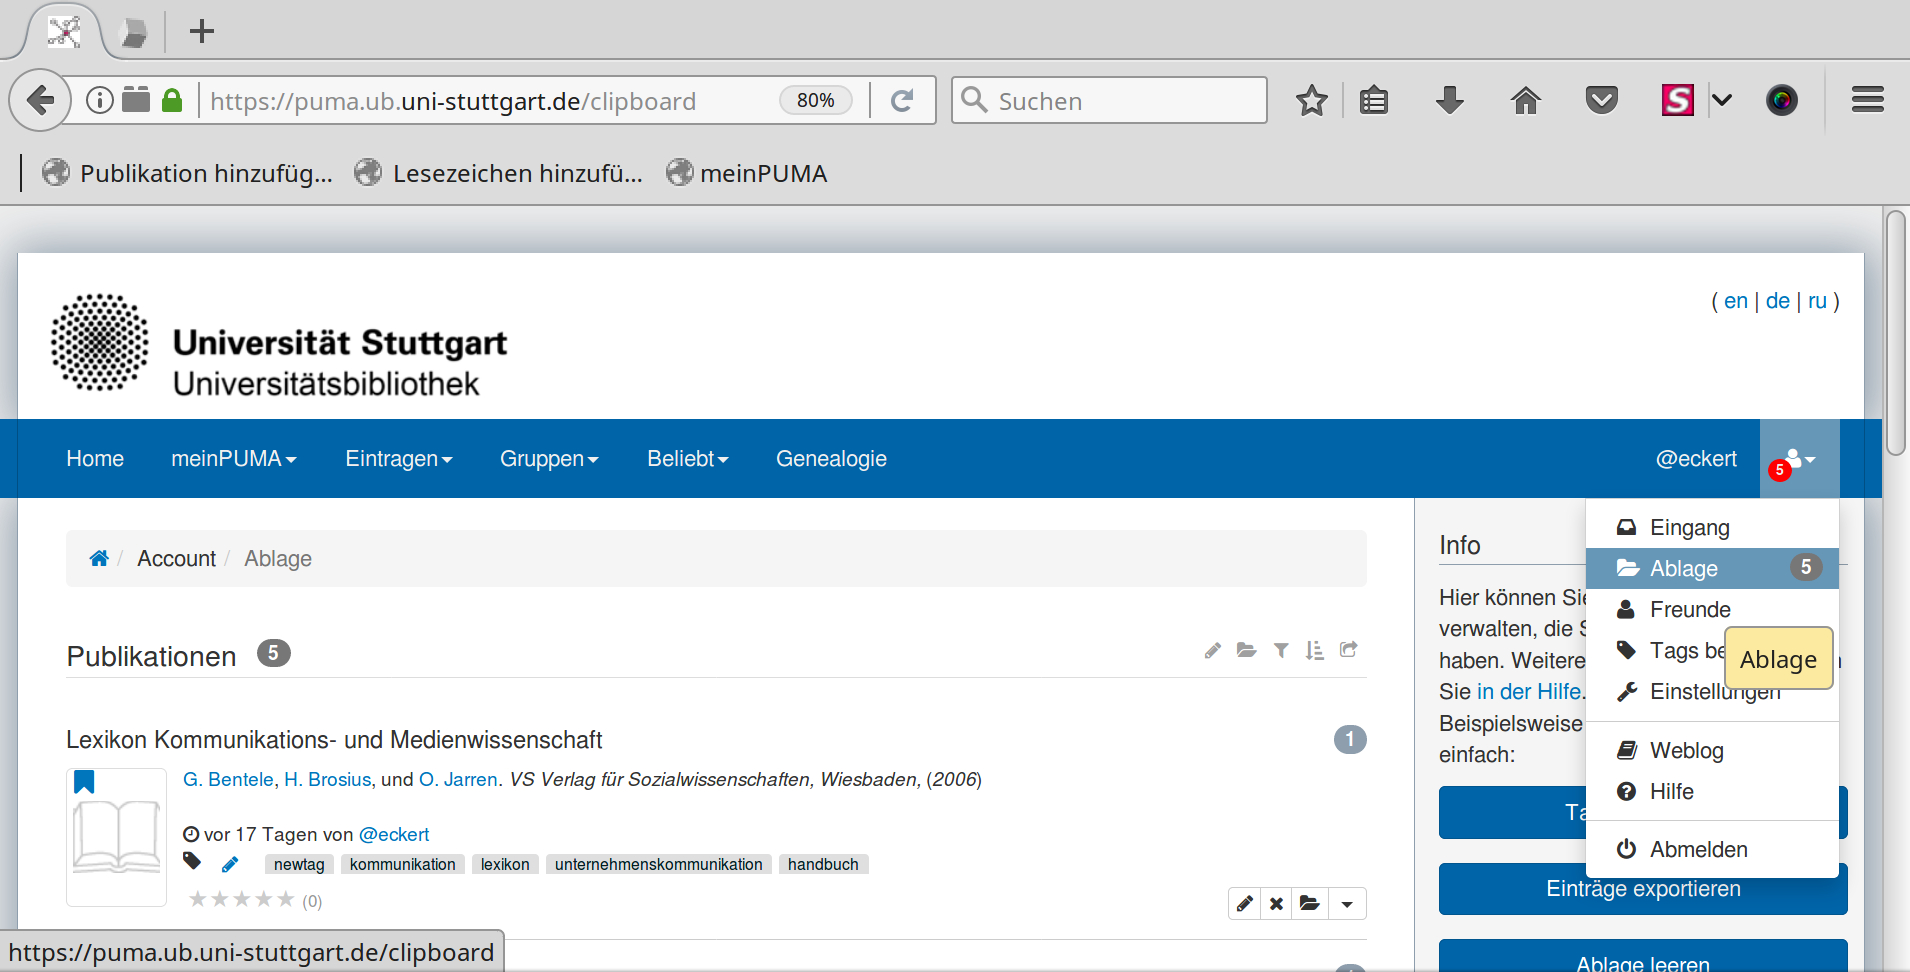
\includegraphics[width=11cm]{Bilder/Kapitel5/Ablage}}
 \caption{Die Ablage}
 \label{fig:ablage}
\end{figure} 
Falls Sie die vorgemerkten Publikationen nicht mehr in der Ablage haben möchten können Sie diese löschen, indem Sie auf das schwarze \enquote{X} (diese Publikation aus Ihrer Sammlung löschen) klicken.\newline
%\begin{wrapfigure}{l}{5cm}
\begin{mdframed}[style=mdfexample1,frametitle={\texttt{ACHTUNG}},backgroundcolor=gray!40]\texttt{Wenn Sie die Publikation in der Ablage löschen ist diese gleichzeitig auch in Ihrer Sammlung gelöscht und kann nicht wiederhergestellt werden.}
\end{mdframed}
%\end{wrapfigure}

Eine andere Möglichkeit ist das Leeren der Ablage. Dies erreichen Sie, indem Sie auf der rechten Seite auf das blaue Feld \enquote{Ablage leeren} klicken. In diesem Fall werden die Publikationen aus der Ablage entfernt, sind aber in Ihrer Sammlung noch vorhanden.
\section{Freischalten erweiterter Funktionen}
\label{sec:freischaltenErweiterterFunktionen}
Bei PUMA gibt es die Unterscheidung zwischen einfachen\index{Funktionen!Einfache} und erweiterten Funktionen\index{Funktionen!Erweiterte}. In den Grundeinstellungen stehen jedem Nutzer, bei dessen Anmeldung bei PUMA, die einfachen Funktionen zur Verfügung. Durch das Freischalten der erweiterten Funktionen kommen weitere Funktionen hinzu, sodass Sie mehr Möglichkeiten haben, PUMA zu nutzen.  Wenn Sie die erweiterten Funktionen freischalten möchten, gehen Sie wie folgt vor:
\begin{enumerate}
    \item Klicken Sie auf das Personensymbol. Ein Dropdown-Menü öffnet sich, klicken Sie auf \enquote{Einstellungen}.
    \item Es öffnet sich die Einstellungs-Seite. Klicken Sie oben auf den Reiter \enquote{Einstellungen}.
    \item Unter dem Bereich \enquote{Layouts Ihrer Tagbox und Ihrer Eintragslisten} befindet sich das Feld \enquote{Erscheinungsbild}. Sie können nun zwischen den Standardeinstellungen \textit{Erweitert} (Alle Optionen werden stets angezeigt) oder \textit{Einfach} (Einige \enquote{Experten}-Optionen werden standardmäßig nicht angezeigt) wählen.
    \begin{figure}[h!]
 \centering
 \fbox{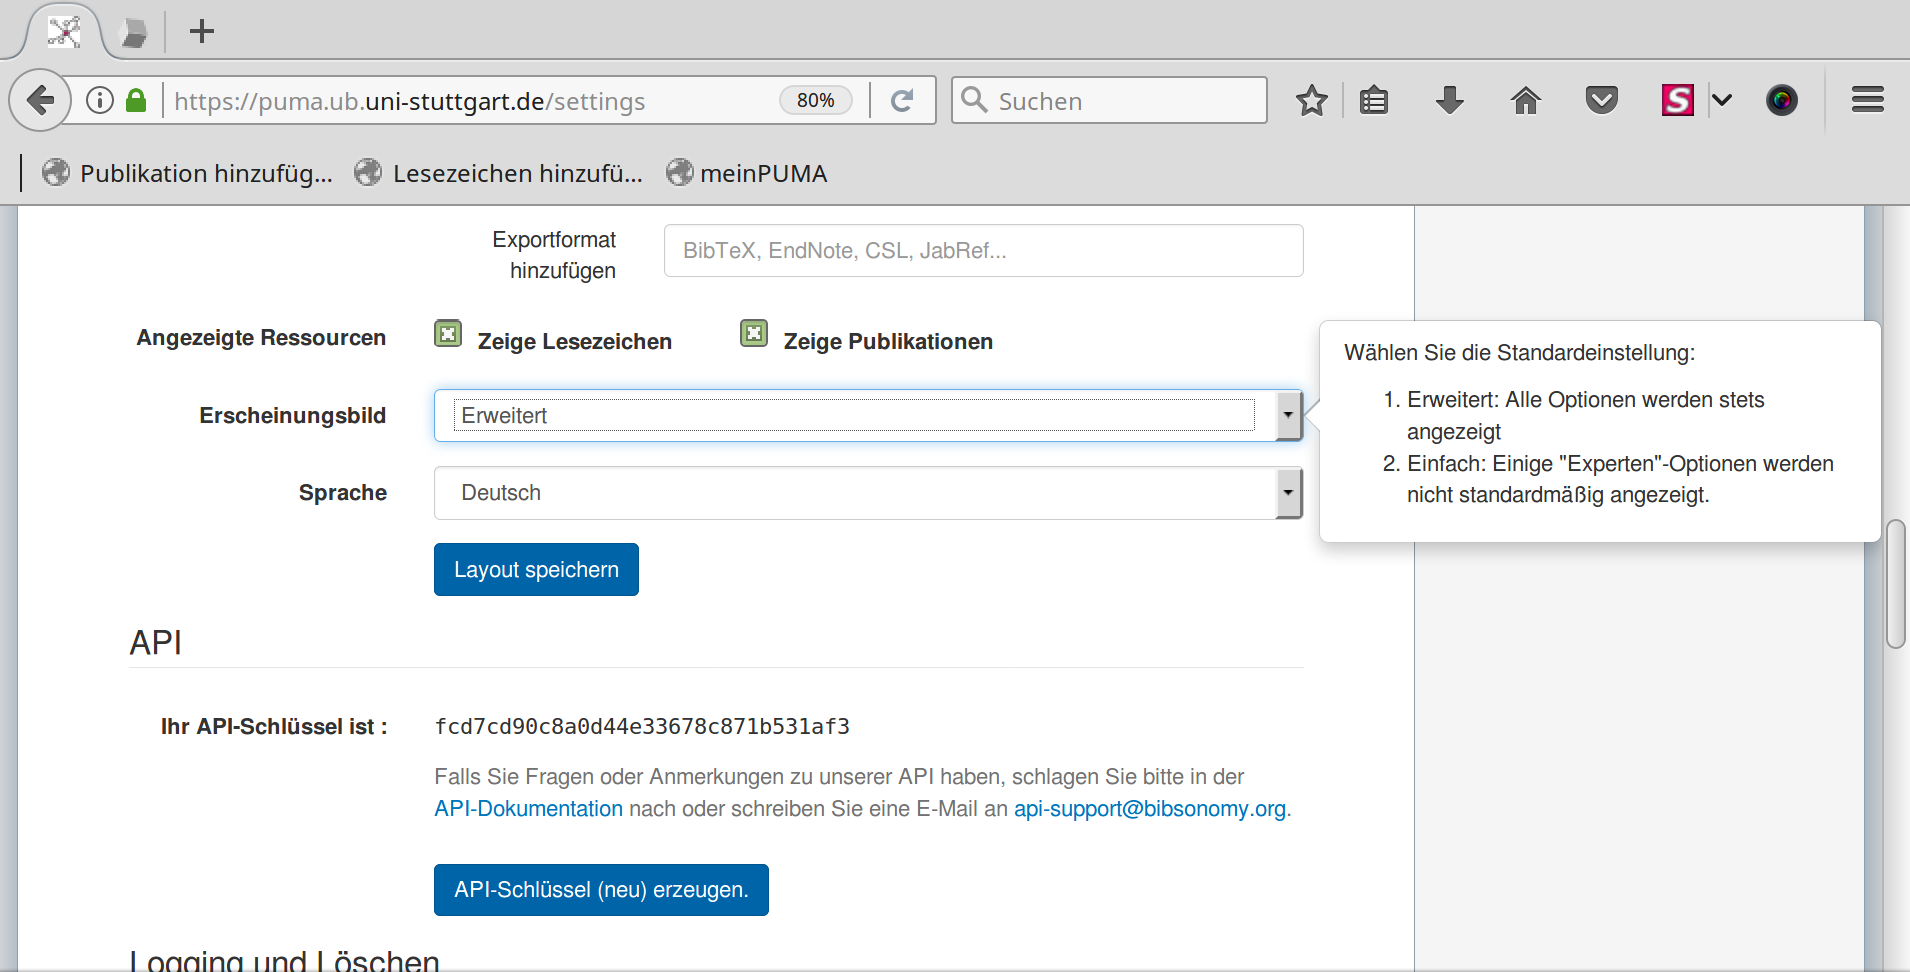
\includegraphics[width=11cm]{Bilder/Kapitel5/Erweiterte_Funktionen}}
 \caption{Erweiterte Funktionen}
 \label{fig:erweiterteFunktionen}
\end{figure} 
    \item Klicken Sie anschließend auf \enquote{Layout speichern}, um Ihre Änderung zu sichern.
\end{enumerate}
\section{Konto auflösen}
\label{sec:kontoAufloesen} 
\subsection{Konto löschen}\index{Konto!löschen} \label{subsec:kontoAufloesen}
\subsection{Ausscheiden aus der Uni}\index{Konto!auflösen} \label{subsec:kontoLoeschen}

\chapter{Erweiterte Funktionen}
\textit{Richtig verwalten ist das A\&O in PUMA. Es geht einfach und spart Zeit.}
\section{Richtig verwalten}

\subsection{Tags/ Schlagwortsystem}
\label{subsec:tags}
Tags\index{Tags} (dt. Schlagwörter) ermöglichen ein übersichtliches Organisieren und Strukturieren der Lesezeichen. Einem Literatureintrag können so viele Tags zu geordnet werden, wie Sie wollen. Durch den Gebrauch von Tags wird die Suche zu einem bestimmten Thema erleichtert, da Sie in die Such-Leiste nur den entsprechenden Tag eingeben müssen und Ihnen werden alle Einträge mit diesem Tag vorgelegt. Ein weiterer Vorteil des Tag-Systems ist, dass Sie bei der Literatursuche Tags kombinieren können und so spezifische Ergebnisse erhalten. So können Sie beispielsweise, wenn Sie Literatur zu dem Thema \enquote{Politik in Deutschland} suchen, die Tags \enquote{Politik} und \enquote{Deutschland} eingeben und erhalten die gesamte Literatur, die sich mit den Themen befasst. 
\begin{figure}[h!]
 \centering
 \fbox{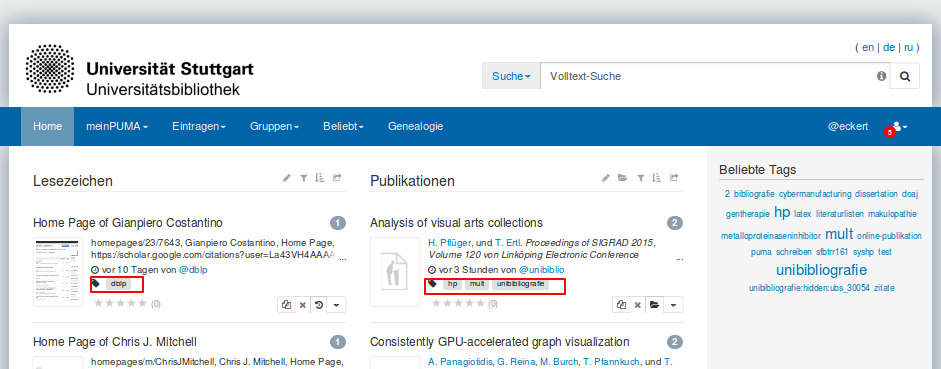
\includegraphics[width=10cm]{Bilder/Kapitel6/Tags}}
 \caption{Tags}
 \label{figure025}
\end{figure}
\textbf{Tags zu Lesezeichen/~Publikationen hinzufügen}\newline
Tags ermöglichen ein übersichtliches Organisieren und Strukturieren der Lesezeichen. Sie können so viele Tags verwenden, wie Sie wollen. Die einzelnen Tags werden durch Leerzeichen voneinander getrennt.
\begin{figure}[h!]
 \centering
 \fbox{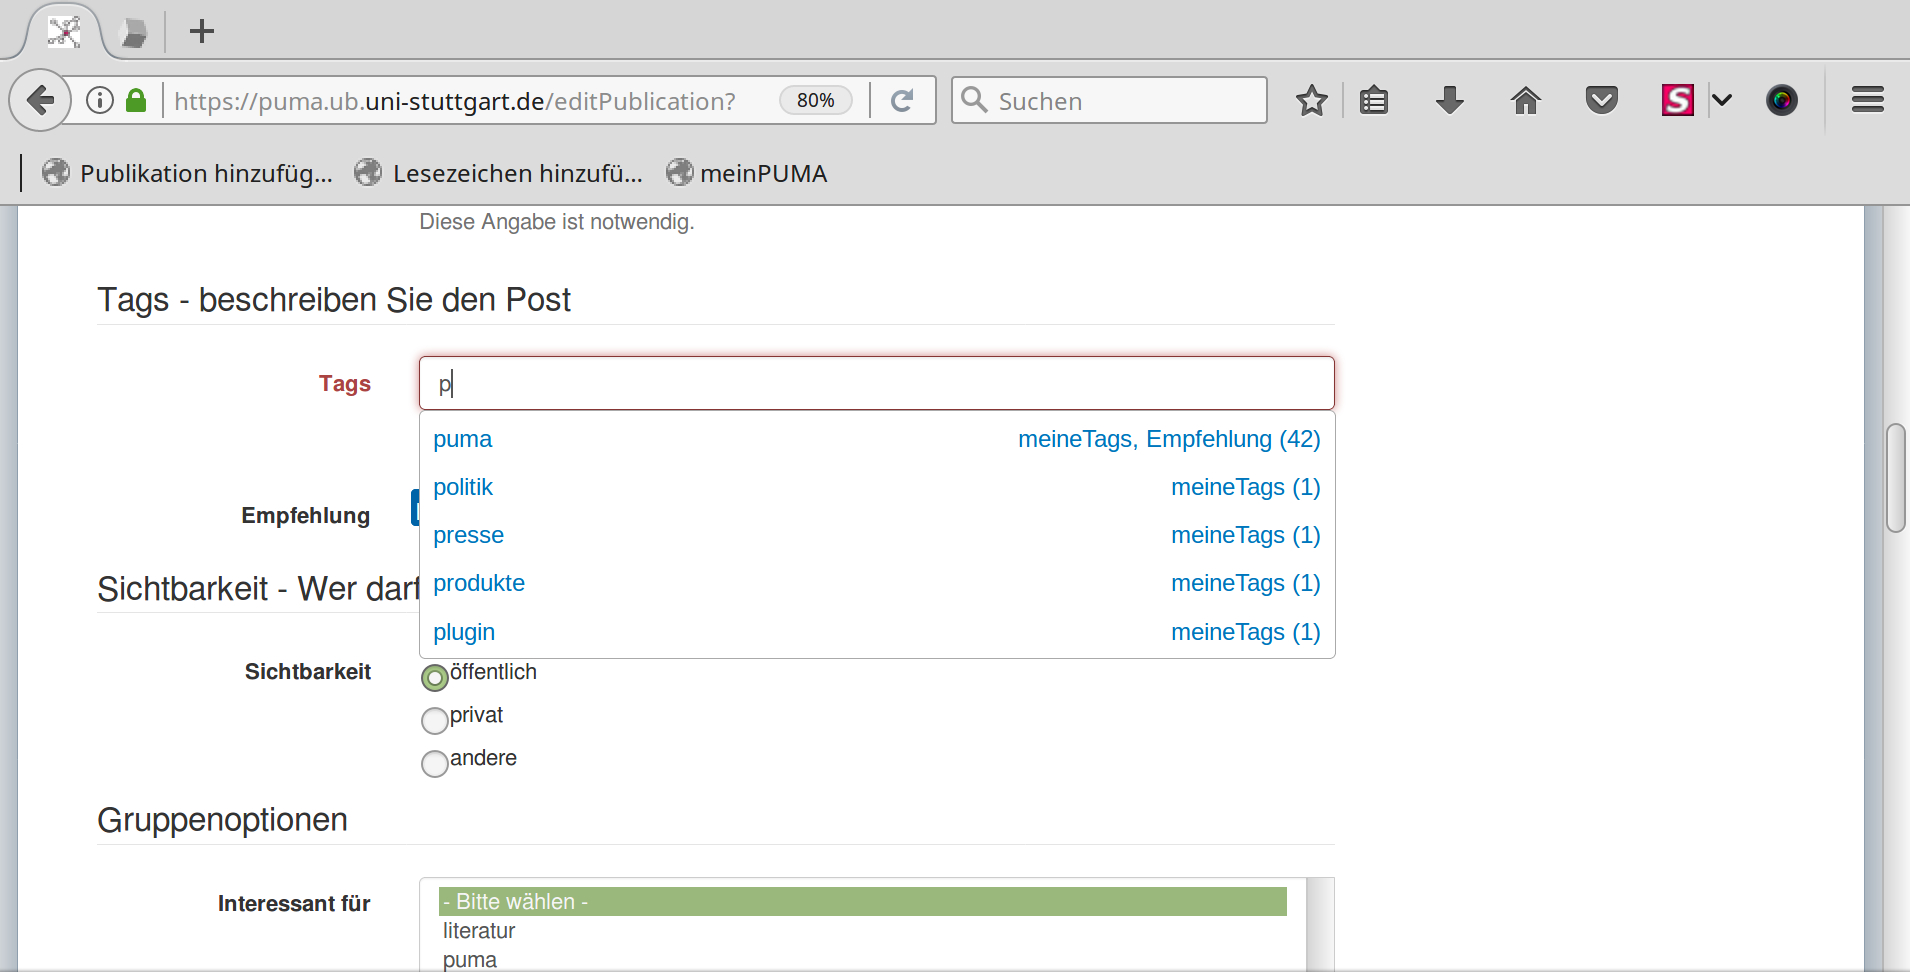
\includegraphics[width=10cm]{Bilder/Kapitel6/Tags_hinzufuegen}}
 \caption{Tags hinzufügen}
 \label{figure026}
\end{figure} 
%\begin{wrapfigure}{l}{7cm}
\begin{mdframed}
[style=mdfexample1,frametitle={\texttt{TIPP}},backgroundcolor=gray!40]
\texttt{Wenn Sie einen Tag verwenden möchten, der aus mehreren Worten besteht (z.~B. Fachbereich Architektur) dann verwenden Sie PascalCase\index{PascalCase} (z.~B. FachbereichArchitektur).} 
\end{mdframed}
%\end{wrapfigure}
\textbf{Tags von Lesezeichen/~Publikationen bearbeiten} \newline
PUMA bietet Ihnen die Möglichkeit bei Publikationen/~Lesezeichen, die schon Teil Ihrer Sammlung sind, die Tags zu bearbeiten. Es gibt drei Möglichkeiten die Tags\index{Tags!bearbeiten} zu bearbeiten:
\begin{enumerate}
    \item \underline{Tags bearbeiten über die \enquote{Schnellbearbeitung}}\newline
    Klicken Sie neben der Publikation/~Lesezeichen auf den blauen Stift (Tags bearbeiten). Es öffnet sich ein Pop-Up-Fenster. Sie können nun alte Tags entfernen, indem Sie auf das \enquote{X-Symbol} klicken. Um neue Tags hinzuzufügen, klicken Sie in das Textfeld und geben die Tags getrennt durch Leerzeichen ein. Um die Änderungen zu speichern klicken Sie auf \enquote{Speichern} und anschließend auf das \enquote{X} um das PopUp-Fenster zu schließen. Wenn Sie die Änderung verwerfen möchten, klicken Sie auf \enquote{Schließen}.
    \item \underline{Tags bearbeiten über \enquote{Eintrag bearbeiten}}\newline
    Klicken Sie auf den schwarzen Stift (Dieses Lesezeichen/Diese Publikation bearbeiten) rechts neben einem Eintrag. Sie können nun die Informationen, die Tags und die Sichtbarkeit des Eintrages bearbeiten. Klicken Sie anschließend auf \enquote{Speichern}.
    \item \underline{Tags bearbeiten über \enquote{Tags bearbeiten}}\newline
    PUMA bietet nicht nur die Möglichkeit die Tags eines einzelnen Eintrags zu bearbeiten, sondern auch alle Tags, die Sie verwenden. Klicken Sie auf das Personensymbol und wählen \enquote{Tags bearbeiten}. Sie können auf dieser Seite Tags und Konzepte\index{Konzepte} bearbeiten:
    \begin{enumerate}
        \item Umbenennen/~Ersetzten von Tags: \newline Hier können Sie alte Tags durch Neue ersetzen. Sie haben so die Möglichkeit, ähnliche Tags zu einem Tag zusammenzufügen.
        \item Subtags zu Konzepten hinzufügen: \newline
        Um ein Subtag zu einem Konzept hinzuzufügen, geben Sie den Namen des Konzepts in das Feld \enquote{Supertag} ein und das Tag, das Sie hinzufügen möchten in das Feld \enquote{Subtag}. Anschließend klicken Sie auf \enquote{Einfügen}.
        \item Subtags von Konzepten löschen:\newline Um ein Subtag von einem Konzept zu löschen, geben Sie den Namen des Konzepts in das Feld \enquote{Supertag} und das Tag, welches Sie löschen wollen, in das Feld \enquote{Subtag} ein. Anschließend klicken Sie auf \enquote{Löschen}.
    \end{enumerate}
\end{enumerate}
\textbf{Suchen\index{Suche} via Tags}\newline
PUMA ermöglicht, dass Sie mit Hilfe der Tags Lesezeichen und Publikationen finden können. \newline\newline
\underline{Möglichkeit 1:} Um einen Eintrag mit einem bestimmten Tag zu finden klicken Sie in der Suchleiste neben \enquote{Suche} auf den blauen Pfeil und wählen im Dropdown-Menü \enquote{Tags} aus. Geben Sie den Tag in das Suchfeld ein und drücken auf das Lupensymbol oder die Enter-Taste.\newline \newline
\underline{Möglichkeit 2:} Wenn Sie bei einem Eintrag auf einen Tag klicken, öffnet sich eine Seite mit allen Einträgen des Nutzer mit diesem bestimmten Tag. Auf der rechten Seite sehen Sie Informationen zu diesen Tag: Der Tag als Tag von allen Nutzern, verwandte Tags, die Konzepte des Nutzers und die verwendeten Tags des Nutzers. 
\newline
\newline
\subsubsection*{Systemtags\index{Systemtags}}
Systemtags\index{Tags!Systemtags} \label{systemtag} sind spezielle Tags, die eine feste Bedeutung haben. Derzeit bietet PUMA drei Typen von Systemtags an:
\begin{description}
\item[Ausführbare Systemtags:]
Ausführbare Systemtags werden zu einem Eintrag hinzugefügt, um eine spezielle Aktion mit diesem Eintrag auszuführen. Sie tragen ausführende Systemtags, wie die anderen Tags, in das Feld \enquote{Tags} ein. 
\begin{enumerate}
    \item \textit{for:<Gruppenname>} : Mit diesem Systemtag kopieren Sie den Eintrag in die Sammlung der Gruppe. In der Gruppe wird der Tag durch \textit{from:<IhrBenutzername>} ersetzt. Wenn Sie ihren Eintrag löschen oder bearbeiten, so bleibt der in die Gruppe kopierte Eintrag unverändert. Nur Mitglieder der Gruppe können Einträge für die Gruppe kopieren.
    \item \textit{send:<Benutzername>} : Damit senden Sie den Eintrag in den Eingang eines anderen Benutzers. Damit dies funktioniert, muss der Empfänger Sie als Freund eingetragen haben oder Sie müssen Mitglied in der gleichen Gruppe sein. Sobald der Eintrag bei dem Nutzer angekommen ist wird der Tag durch \textit{sent:<Benutzername>} ersetzt.
\end{enumerate}
\item[Meta-Systemtags:]  
Mit Meta-Systemtags markieren Sie Einträge. Derzeit werden folgende Meta-Systemtags unterstützt:
\begin{enumerate}
    \item \textit{myown:} Ein Eintrag, der mit dem Tag myown\index{myown} versehen wurde, erscheint auf Ihrer CV-Seite. Durch den Tag geben Sie an, dass Sie der Verfasser des Lesezeichen/der Publikation sind.
    \item \textit{sys:relevantFor:<Gruppenname>} : Einträge mit dem Tag sys:relevantFor:xy werden auf der \enquote{Interessant für\index{Interessant für}}-Seite der Gruppe xy angezeigt. Damit hat dieser Tag den gleichen Effekt, wie das  Auswählen der Gruppe xy in der \enquote{Interessant für}-Box beim Bearbeiten eines Eintrages. Der Tag wird durch eine blaue Blume am Anfang der Tag-Reihe dargestellt. 
    \item \textit{sys:hidden:<tag>} : Der Tag ist nur für Sie selbst sichtbar. Man findet diesen Tag bei einer Publikation, die im Inhaltsbereich abgebildet wird, nicht sichtbar in der Reihe der anderen Tags. Der Tag wird durch eine blaue Blume am Anfang der Tag-Reihe dargestellt. Wenn Sie auf die Detailansicht der Publikation klicken, taucht er sichtbar in der Tag-Reihe auf.
\end{enumerate}
\item[Such-Systemtags:] 
\label{itm:suchSystemtag}
Such-Systemtags sind nicht dazu da, um in einen Eintrag geschrieben zu werden, sondern um Einträge nach Suchanfragen zu filtern. Alle Such-Systemtags haben die gleiche Syntax: \textit{sys:<Feldname>:<Feldwert>}. Beispielsweise werden  bei der Suchanfrage \textit{sys:author:xyz} nur die Einträge angezeigt, welche von dem Autor \textit{xyz} stammen.\newline
Die Syntax kann entweder in die Suchleiste oder mit der URL eingeben werden. Folgende Filter unterstützt PUMA (Suche beschränkt sich auf die Publikationseinträge):\newline
\newline
Für die Suche nach einem bestimmten Autor oder Erscheinungsjahr müssen Sie vorher festlegen, in welchen Einträgen eines Nutzers Sie nach dem Autor oder dem Erscheinungsjahr suchen möchten. Zum Beispiel suchen Sie, wenn Sie diese Daten eingeben: \newline https://puma.ub.uni-stuttgart.de/user/\newline droessler/sys:year:2013 \newline Publikationen aus dem Jahr 2013 in den Einträgen des Nutzers Droessler. 
\begin{enumerate}
    \item \textit{sys:author:<Autorenname>} filtert die Suche nach dem Autor.
    \item \textit{sys:year:<Jahr>} filtert die Suche nach dem Erscheinungsjahr. Dabei sind mehrere Schreibweisen für das Jahr möglich:
    \begin{enumerate}
        \item 2000: Alle Einträge aus dem Jahr 2000
        \item 2000-: Alle Einträge aus dem Jahr 2000 oder einem Jahr danach
        \item -2000: Alle Einträge aus dem Jahr 2000 oder einem Jahr davor
        \item 1990-2000: Alle Einträge aus den Jahren 1990 bis 2000
    \end{enumerate}
%muss noch raus rutschen
Bei der Suche nach Titel, Gruppe, Nutzer, usw. spielt der Nutzer, bei dem Sie suchen keine Rolle. Sie müssen dementsprechend nur den Zusatz tag/ vor die Suchsyntax setzten, zum Beispiel  https://puma.ub.uni-stuttgart.de/tag/sys:entrytype:article. Hier finden Sie nun alle Artikel, die auf PUMA eingetragen wurden.
    \item \textit{sys:title:<title>} sucht nach Einträgen mit diesem Titel.
    \item \textit{sys:user:<user>} sucht nach Einträgen eines Nutzers.
    \item \textit{sys:group:<group>} filtert die Suche nach einer bestimmten Gruppe.
    \item \textit{sys:entrytype:<Eintragstyp>} filtert die Suche nach dem Eintragstypen. Eintragstypen\footnote{\url{https://www.ctan.org/pkg/biblatex?lang=de}} werden verwendet, um BibTex-Einträge nach ihren Typen zu klassifizieren. Derzeit unterstützt Puma folgende Eintragstypen\index{Eintragstypen}: 
    \begin{enumerate}
        \item \textbf{article\index{Article}:} Zeitungs- oder Zeitschriftenartikel\newline
        Erforderliche Felder: Autor, Titel, Zeitschriftentitel, Ausgabennummer, Jahr/Datum 
        \item \textbf{book\index{Book}:} Buch, Monografie mit angegebenem Verlag\newline
        Erforderliche Felder: Autor, Titel, Jahr
        \item \textbf{booklet\index{Booklet}:} Gebundenes Druckwerk, aber ohne Verlag oder Sponsororganisation\newline
        Erforderliche Felder: Autor/Lektor, Titel, Jahr/Datum
        \item \textbf{conference\index{Conference}:} Ein Beitrag zu einer Konferenz, der nicht in einem Konferenzband erschienen ist\newline
        Erforderliche Felder: Autor, Titel, Buchtitel, Jahr/Datum
        \item \textbf{electronic\index{Electronic}:} Elektronische Veröffentlichungen, z. B. eBooks oder Blogeinträge\newline 
        Erforderliche Felder: Autor, Buchtitel, Verlag, Adresse, Jahr
        \item \textbf{inbook\index{Inbook}:} Teil eines Buches, z. B. ein Kapitel oder ein Seitenbereich\newline
        Erforderliche Felder: Autor, Titel, Buchtitel, Jahr/Datum 
        \item \textbf{incollection\index{Incollection}:} Teil eines Buches mit einem eigenem Titel, z. B. Beitrag in einem Sammelband\newline
        Erforderliche Felder: Autor, Titel, Buchtitel, Jahr/Datum
        \item \textbf{inproceedings\index{Inproceedings}:} Artikel in einem Tagungsband bzw. Konferenzband\newline
        Erforderliche Felder: Autor, Titel, Buchtitel, Jahr/Datum
        \item \textbf{manual\index{Manual}:} Technische Dokumentation, Handbuch\newline
        Erforderliche Felder: Autor/Lektor, Titel, Jahr/Datum
        \item \textbf{mastersthesis\index{Mastersthesis}:} Master-, Magister- oder Diplomarbeit\newline
        Erforderliche Felder: Autor, Titel, Art der Arbeit, Institut, Jahr/Datum
        \item \textbf{misc\index{Misc}:} Diesen Eintragstyp können Sie wählen, wenn nichts anderes zu passen scheint. \newline
        Erforderliche Felder: Autor/Lektor, Titel, Jahr/Datum
        \item \textbf{patent\index{Patent}:} Patent\newline 
        Erforderliche Felder: Autor, Titel, Nummer, Jahr/Datum
        \item \textbf{periodical\index{Periodical}:} Ein regelmäßig erscheinendes Werk, z.B. Zeitschrift\newline
        Erforderliche Felder: Lektor, Titel, Jahr/Datum
        \item \textbf{phdthesis\index{Phdthesis}:} Doktor- oder andere Promotionsarbeit\newline 
        Erforderliche Felder: Autor, Titel, Hochschule/Universität, Jahr 
        \item \textbf{presentation\index{Presentation}:} Präsentation, Vortrag auf einer Veranstaltung\newline 
        Erforderliche Felder: Verfasser, Titel, Anlass der Präsentation, Jahr
        \item \textbf{proceedings\index{Proceedings}:} Tagungsband einer Konferenz\newline
        Erforderliche Felder: Titel, Jahr/Datum
        \item \textbf{standard\index{Standard}:} Standard\newline 
        Erforderliche Felder: Autor, Buchtitel, Verlag, Adresse, Jahr 
        \item \textbf{techreport\index{Techreport}:} Bericht einer Hochschule oder einer anderen Institution\newline
        Erforderliche Felder: Autor, Titel, Jahr/Datum
        \item \textbf{unpublished\index{Unpublished}:} Nicht formell veröffentlichtes Dokument\newline 
        Erforderliche Felder: Autor, Titel, Jahr/Datum
    \end{enumerate}
    \item \textit{sys:not:<tag>} filtert die Suche, indem alle Ergebnisse ignoriert werden, die diesen Tag enthalten. An dieser Stelle können Sie auch Platzhalter verwenden, z.B. werden bei sys:not:news\_ 
    alle Ergebnisse ignoriert, die Tags enthalten, die mit news\_
    beginnen.
    \item \textit{sys:bibtexkey:<bibtexkey>} filtert die Suche nach einem bestimmten BibTeX-Schlüssel.
\end{enumerate}
\end{description}
\subsection{Konzepte}
\underline{Was sind Konzepte\index{Konzepte}?}
\newline
Durch Konzepte können Sie Ihre Tags nach Gruppen ordnen und sich so die Suche erleichtern. Sie haben beispielsweise das Konzept mit dem Supertag\index{Supertag} (Namen) Obst, diesem sind die Subtags\index{Subtag} Banane, Apfel und Kiwi zugeordnet. Wenn Sie nun mit dem Konzept Obst suchen, werden Ihnen automatisch alle Publikationen und Lesezeichen angezeigt, die mit mindestens einem der Subtags getagged wurden. Dies erleichtert Ihre Suche, da oft nach Publikationen/Lesezeichen zu einem bestimmten Thema gesucht wird. 
\newline Ihre angelegten Konzepte finden Sie über das Untermenü von \enquote{mein PUMA}. Um zu den beliebten Konzepten von PUMA zu gelangen klicken Sie im Hauptmenü auf \enquote{Beliebte} und anschließend im Untermenü auf \enquote{Konzepte}. 
\newline
\newline
\underline{Konzepte erstellen}
\newline
Um Konzepte zu erstellen oder zu überarbeiten, klicken Sie auf das Personensymbol auf der rechten Seite. Ein Untermenü öffnet sich und Sie klicken auf Tags bearbeiten. 
\begin{figure}[h!]
 \centering
 \fbox{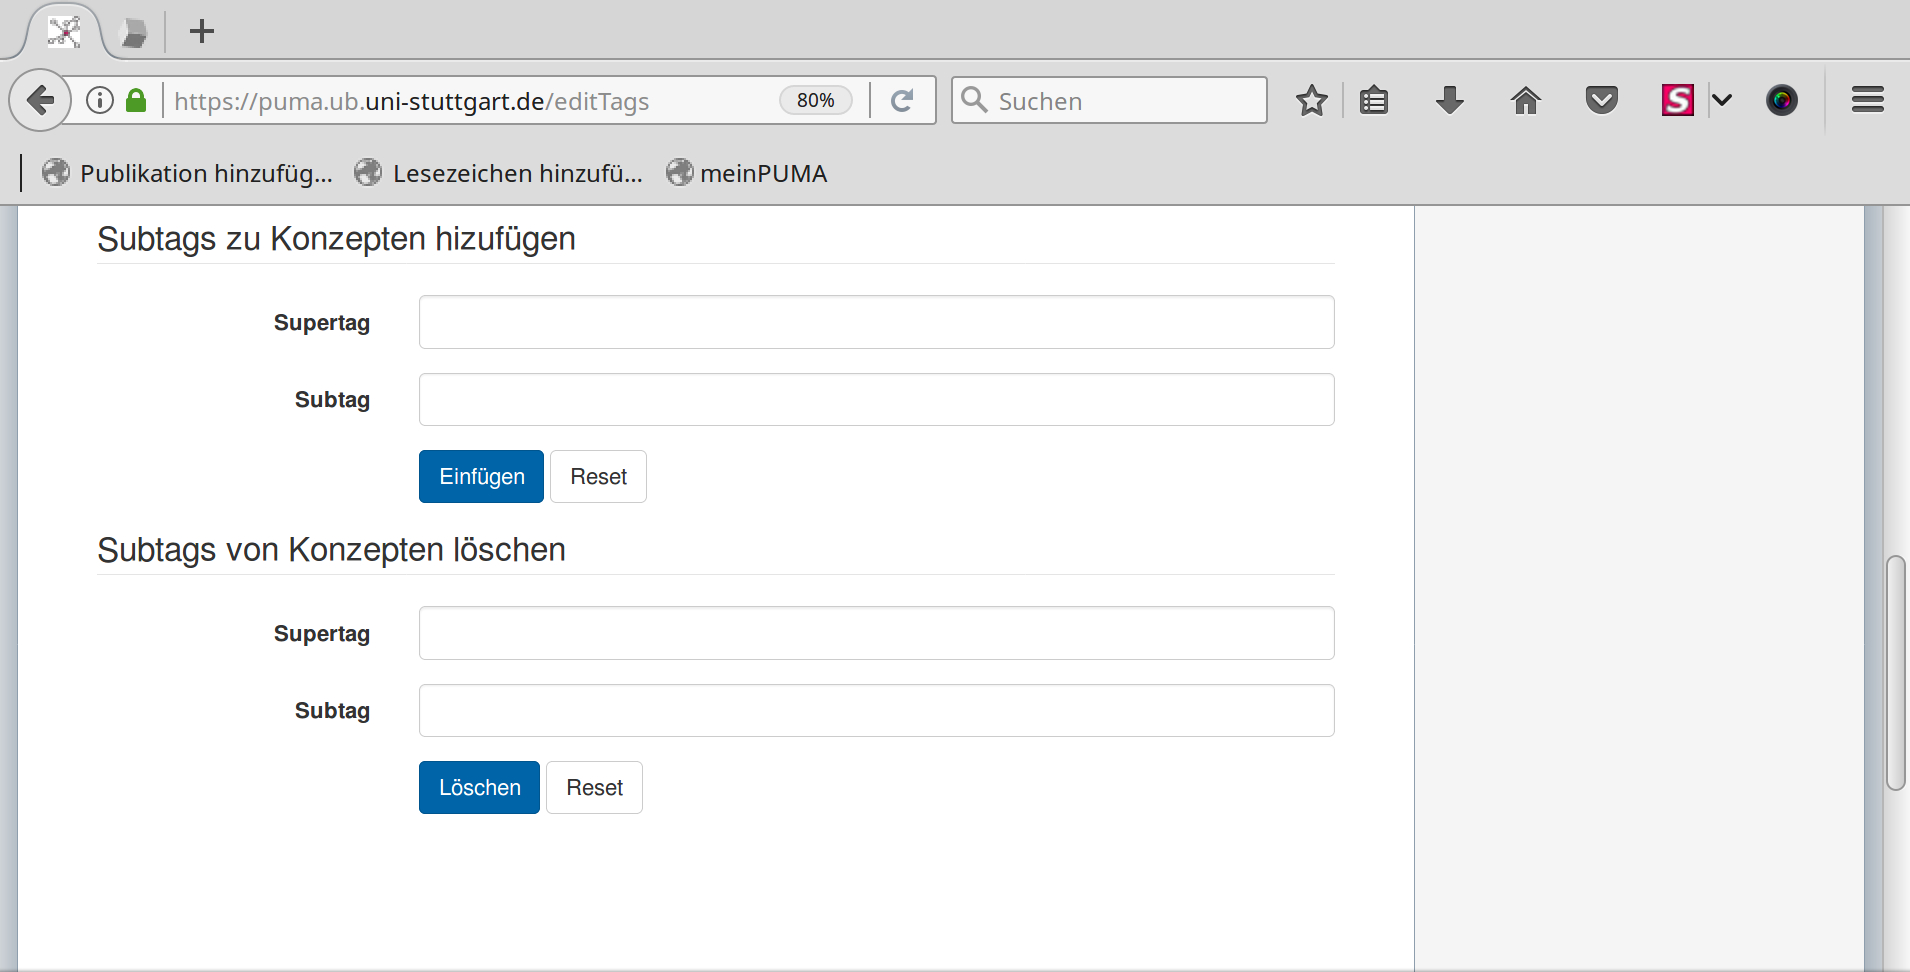
\includegraphics[width=10cm]{Bilder/Kapitel6/Konzepte_erstellen}}
 \caption{Ein Konzept erstellen}
 \label{figure027}
\end{figure}
\textbf{Subtags zu Konzepten hinzufügen:} PUMA ermöglicht Ihnen neue Konzepte zu erstellen oder zu einem bereits existierenden Konzept neue Tags hinzufügen. Um ein neues Konzept hinzuzufügen, wählen Sie einen Tag, der als Name für das Konzept stehen soll, aus. Diesen Tag geben Sie in das Feld \enquote{Supertag} ein. Den Tag, der dem Konzept hinzugefügt werden soll, geben Sie in das Feld \enquote{Subtag} ein.
\begin{mdframed}[style=mdfexample1,frametitle={\texttt{ACHTUNG}},backgroundcolor=gray!40]\texttt{Es kann immer nur ein Subtag eingegeben werden, wenn Sie zwei Subtags gleichzeitig eingeben wird das Konzept nicht erstellt. Um mehrere Subtags in einem Konzept zu vereinen, müssen sie den oben genannten Ablauf zur Erstellung eines Konzeptes mit jedem neuen Subtag wiederholen und dabei das Supertag unverändert lassen.} 
\end{mdframed}
\textbf{Subtags von Konzept löschen:} Sie können auch Tags aus einem Konzept entfernen. Dafür geben Sie in das Feld \enquote{Supertag} den Namen des Konzepts ein und in das Feld \enquote{Subtag} den Tag, der gelöscht werden soll. 
\begin{mdframed}[style=mdfexample1,frametitle={\texttt{ACHTUNG}},backgroundcolor=gray!40]\texttt{Hier kann ebenfalls immer nur ein Tag in das Feld Subtag eingegeben werden, da sonst die Aktion nicht durchgeführt wird.}
\end{mdframed}
\underline{Navigation mit Konzepten}
\newline
Um mit Konzepten zu suchen, benutzen Sie einfach die Suchleiste rechts oben. Klicken Sie auf den blauen Pfeil neben \enquote{Suche} und wählen Sie im Dropdown-Menü Konzepte aus. Geben Sie den Namen des Konzepts, mit dem Sie suchen möchten, in das Suchfeld ein und klicken Sie auf das Lupensymbol oder drücken Sie die Enter-Taste. Die Lesezeichen/Publikationen, die mit einem der Subtags des Konzepts getagged worden sind, werden Ihnen angezeigt. 
\subsection{Duplikate}
Beim Sammeln von Publikationen und Lesezeichen kann es vorkommen, dass Publikationen zweimal in eine PUMA-Sammlung eintragen werden. Hier bietet PUMA die Möglichkeit Duplikate\index{Duplikate} sofort zu erkennen und seine Sammlung aufzuräumen. Um einen Überblick über alle Duplikate in seiner Sammlung zu erhalten, klicken Sie im Hauptmenü auf \enquote{meinPuma}. Im Dropdown-Menü können Sie nun \enquote{Duplikate} auswählen und gelangen so auf die Übersichtsseite. Ein anderer Weg, um sich einen Überblick zu verschaffen, bieten die Zahlen oben rechts bei jedem Eintrag. Sie geben an, wie viele Einträge mit dem gleichen Titel es in der Sammlung gibt. Ist diese Zahl größer als 1 handelt es sich um Duplikate. Wenn Sie auf die Zahl klicken werden Ihnen die Duplikate angezeigt.
\begin{figure}[h!]
 \centering
 \fbox{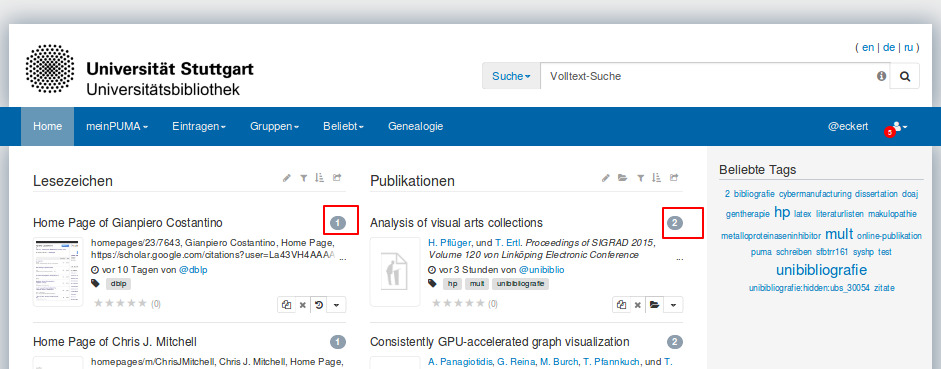
\includegraphics[width=10cm]{Bilder/Kapitel6/Duplikate}}
 \caption{Duplikate}
 \label{figure027}
\end{figure}
\subsection{Private Dateien anhängen}
Sie können an jede Ihrer Publikationen ein Dokument\index{Dokumente! anhängen} anhängen (max. 50 MB pro Datei - erlaubte Dateiendungen: pdf, ps, djv, djvu, txt, tex, doc, docx, ppt, pptx, xls, xlsx, ods, odt, odp, jpg, jpeg, svg, tif, tiff, png, htm, html, epub). Der Anhang ist aus urheberrechtlichen Gründen nur für Sie selbst sichtbar.

\begin{mdframed}[style=mdfexample1,frametitle={\texttt{BEDINGUNG}},backgroundcolor=gray!40]\texttt{Um an eine Publikation eine Datei anzuhängen, muss die Publikation in Ihrer Sammlung eingetragen sein.}\end{mdframed}
\begin{enumerate}
    \item Klicken Sie auf den Titel der Publikation. Es öffnet sich die Detailansicht der Publikation.
    \item Klicken Sie nun entweder auf den schwarzen Stift oben rechts auf der Seite. Es öffnet sich eine neue Seite, auf der Sie die Publikation bearbeiten können. Scrollen Sie runter bis zu \enquote{private Dokumente} und klicken auf \enquote{Durchsuchen}. \newline \textbf{ODER:} Sie klicken in der Detailansicht auf das Bild der Publikation. Unterhalb des Bildes erscheint der Durchsuchen-Button. 
    \item Es öffnet sich ein Pop-Up Fenster, indem Sie das Dokument auswählen können, welches Sie anhängen wollen. Klicken Sie anschließend auf \enquote{Öffnen}.
    \item Der Upload startet automatisch. Sobald er abgeschlossen ist, wird der Dateienname der hochgeladenen Datei und ein schwarzes \enquote{X} unter dem Abschnitt \enquote{private Dokumente} angezeigt. Über das schwarze \enquote{X} kann das Dokument wieder entfernt werden.
    \item Klicken Sie anschließend ganz unten auf der Seite auf \enquote{Speichern}, da ansonsten Ihre Änderung nicht gespeichert wird.
\end{enumerate}
\begin{figure}[h!]
 \centering
 \fbox{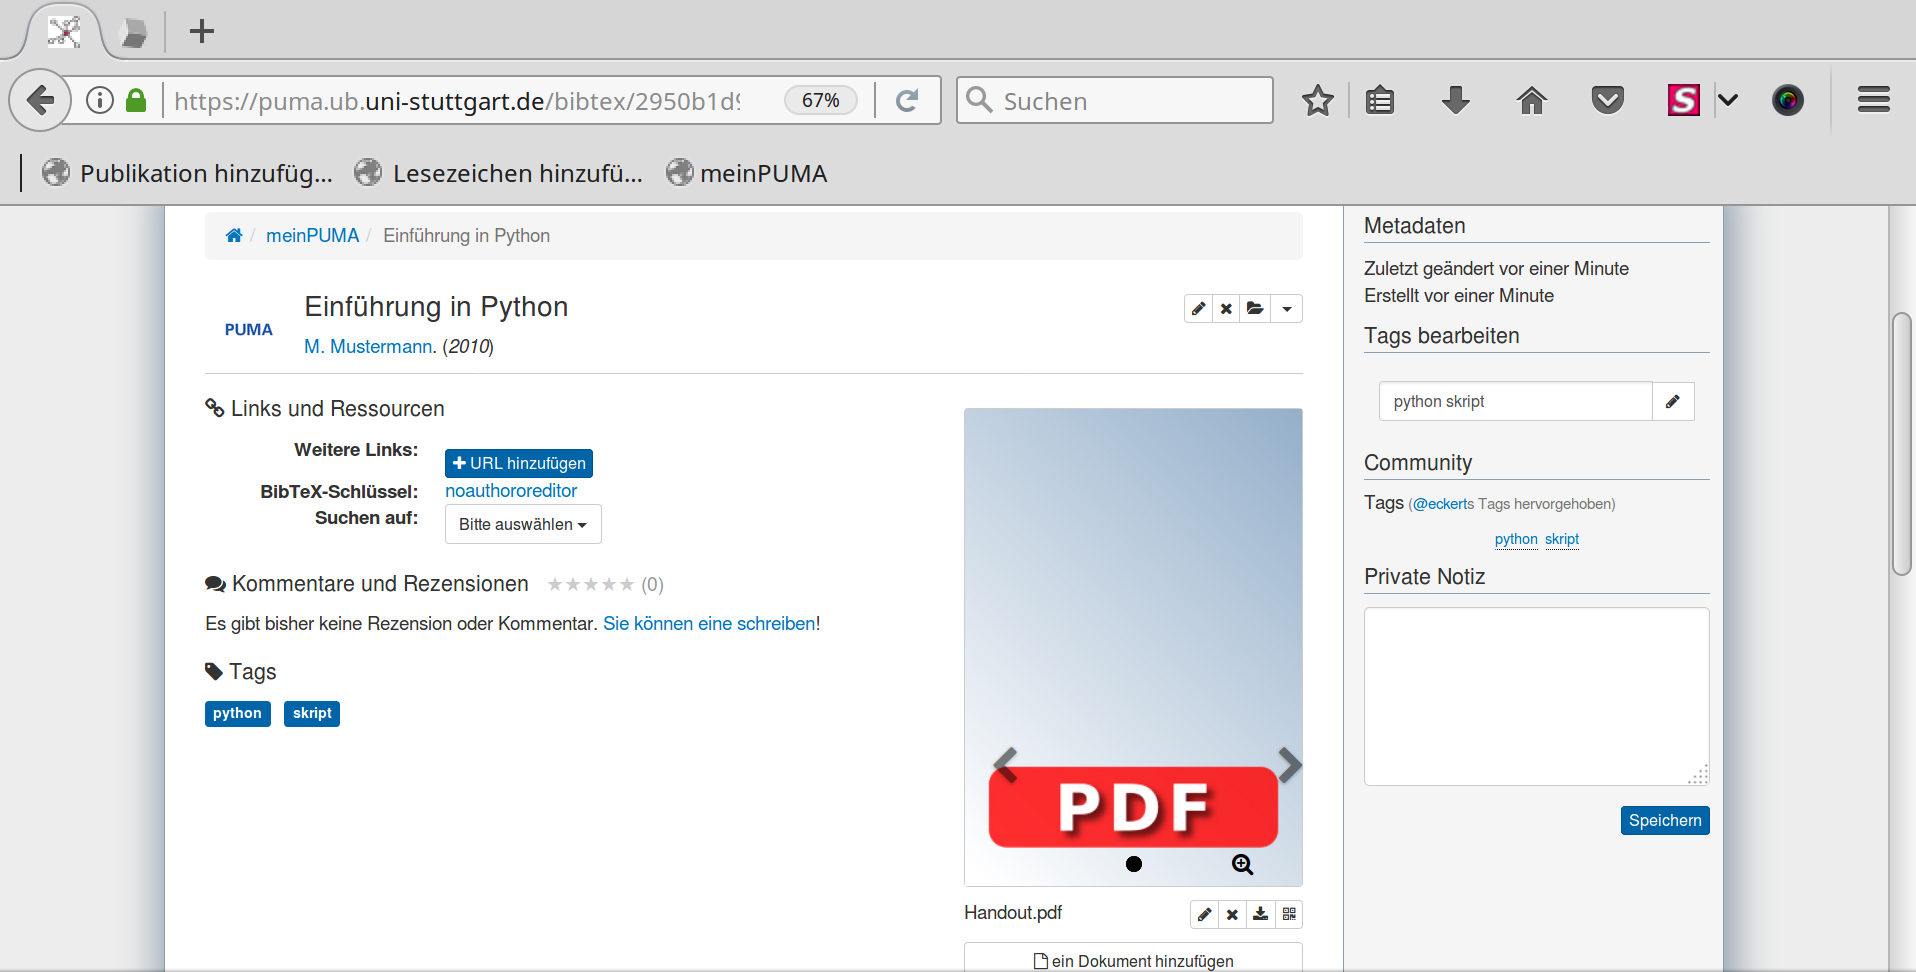
\includegraphics[width=10cm]{Bilder/Kapitel6/Private_Dokumente}}
 \caption{Private Dokumente anhängen}
 \label{figure028}
\end{figure}
Wenn die angehängte Datei auch für Gruppenmitglieder sichtbar seien soll, muss der  Gruppenadministrator das Teilen von Dokumenten erlauben
und die einzelnen Mitglieder dies ebenfalls in ihrer Gruppeneinstellung freischalten. In den Einstellungen kann der Nutzer unter dem Reiter \enquote{Gruppen} für jede einzelne Gruppe festlegen, ob Dateien geteilt werden oder nicht. Diese Funktion kann jederzeit wieder deaktiviert werden.
\subsection{Publikationen durchstöbern}
Oftmals verliert man schnell den Überblick über seine Einträge. Um sich schnell einen Überblick über seinen Literaturbestand machen zu können bietet PUMA die Funktion \enquote{Publikation\index{Publikationen!durchstöbern} durchstöbern} an. 
\begin{enumerate}
    \item Klicken Sie im Hauptmenü auf \enquote{meinPUMA}. Ein Dropdown-Menü öffnet sich.
    \item Klicken Sie auf \enquote{Publikationen durchstöbern}.
    \item Unter \enquote{Suchoptionen} können Sie verschiedene Tags und Autoren auswählen, zu denen Sie die Einträge sehen möchten. Um mehrere Begriffe aus der Liste auszuwählen, halten Sie die STRG- bzw. CTRL-Taste während des Mausklicks gedrückt.
\begin{figure}[h!]
 \centering
 \fbox{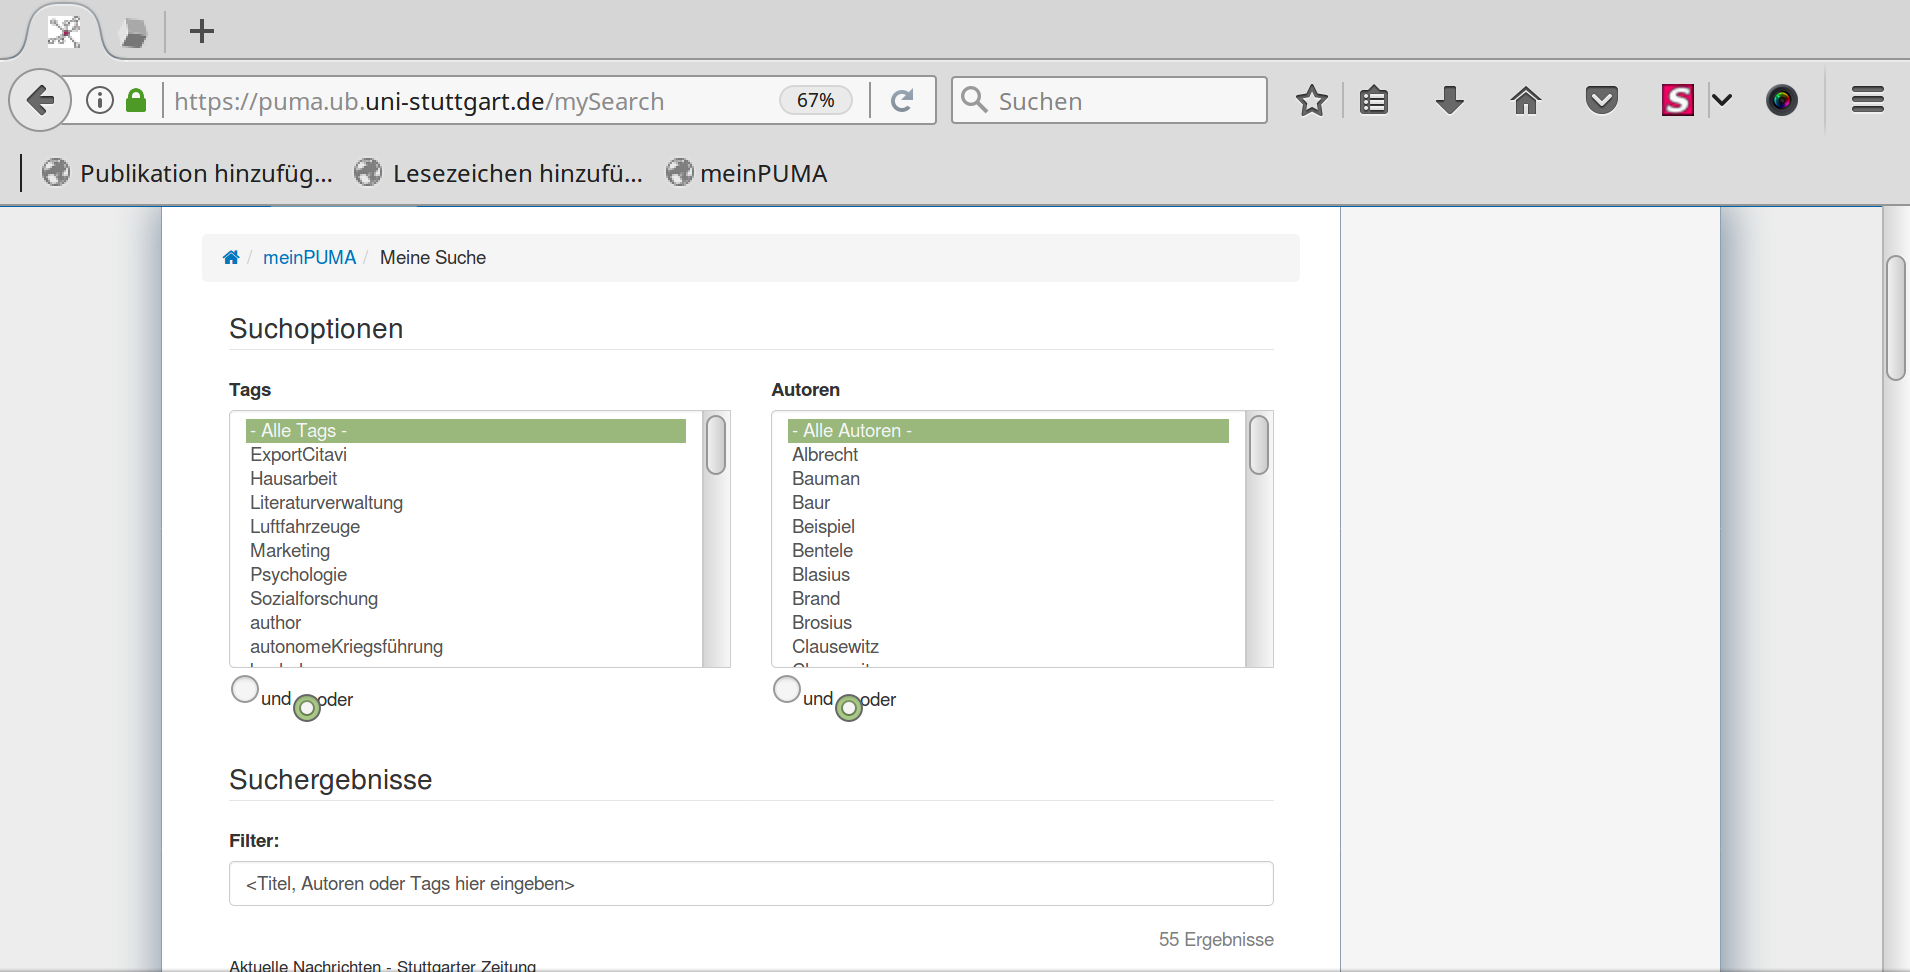
\includegraphics[width=10cm]{Bilder/Kapitel6/Publikationen_durchstoebern}}
 \caption{Publikationen durchstöbern}
 \label{figure029}
\end{figure}
    \item Die Buttons \enquote{und/~oder} können Sie dazu nutzen, um die Listenauswahl unterschiedlich zu verknüpfen. 
    \item Unter \enquote{Suchergebnisse} sehen Sie alle Ergebnisse, die zu ihren Vorgaben aus 3. und 4. passen.
    \item Das Textfeld \enquote{Filter} ermöglicht es die Ergebnisse aus Schritt 5 noch weiter zu filtern.
\end{enumerate}
\subsection{Eigene Einträge bearbeiten}
Ist ein Eintrag einmal hinzugefügt, heißt dies nicht, dass man ihn nie mehr bearbeiten kann. Die erste Möglichkeit wäre, dass der Nutzer jeden Eintrag selber von Hand nachträglich bearbeitet. Die zweite Lösung ist zeitsparender und schneller.\newline
In der Sammlung befindet sich oben rechts oberhalb der Publikations- und Lesezeichenspalte ein Stift, mit dem Sie Ihre eigenen Eintrage bearbeiten können. Durch das Klicken auf den Stift gelangen Sie auf die Seite \enquote{Eigene Einträge bearbeiten}. Hier können Sie auswählen, was Sie an der/~den Publikation/~en ändern möchten:
\begin{itemize}
\item Tags zu allen ausgewählten Posts hinzufügen
\item Die Tags aller ausgewählten Einträge separat bearbeiten
\item BibTex-Schlüssel normalisieren
\item Einträge löschen
\item Sichtbarkeit einstellen
\end{itemize}
Die Änderungen können für eine Publikation/Lesezeichen oder mehrere sein. Dies können Sie unten auf der Seite festlegen. Durch klicken auf die entsprechenden Einträge wählen Sie diese aus.
\begin{figure}[h!]
 \centering
 \fbox{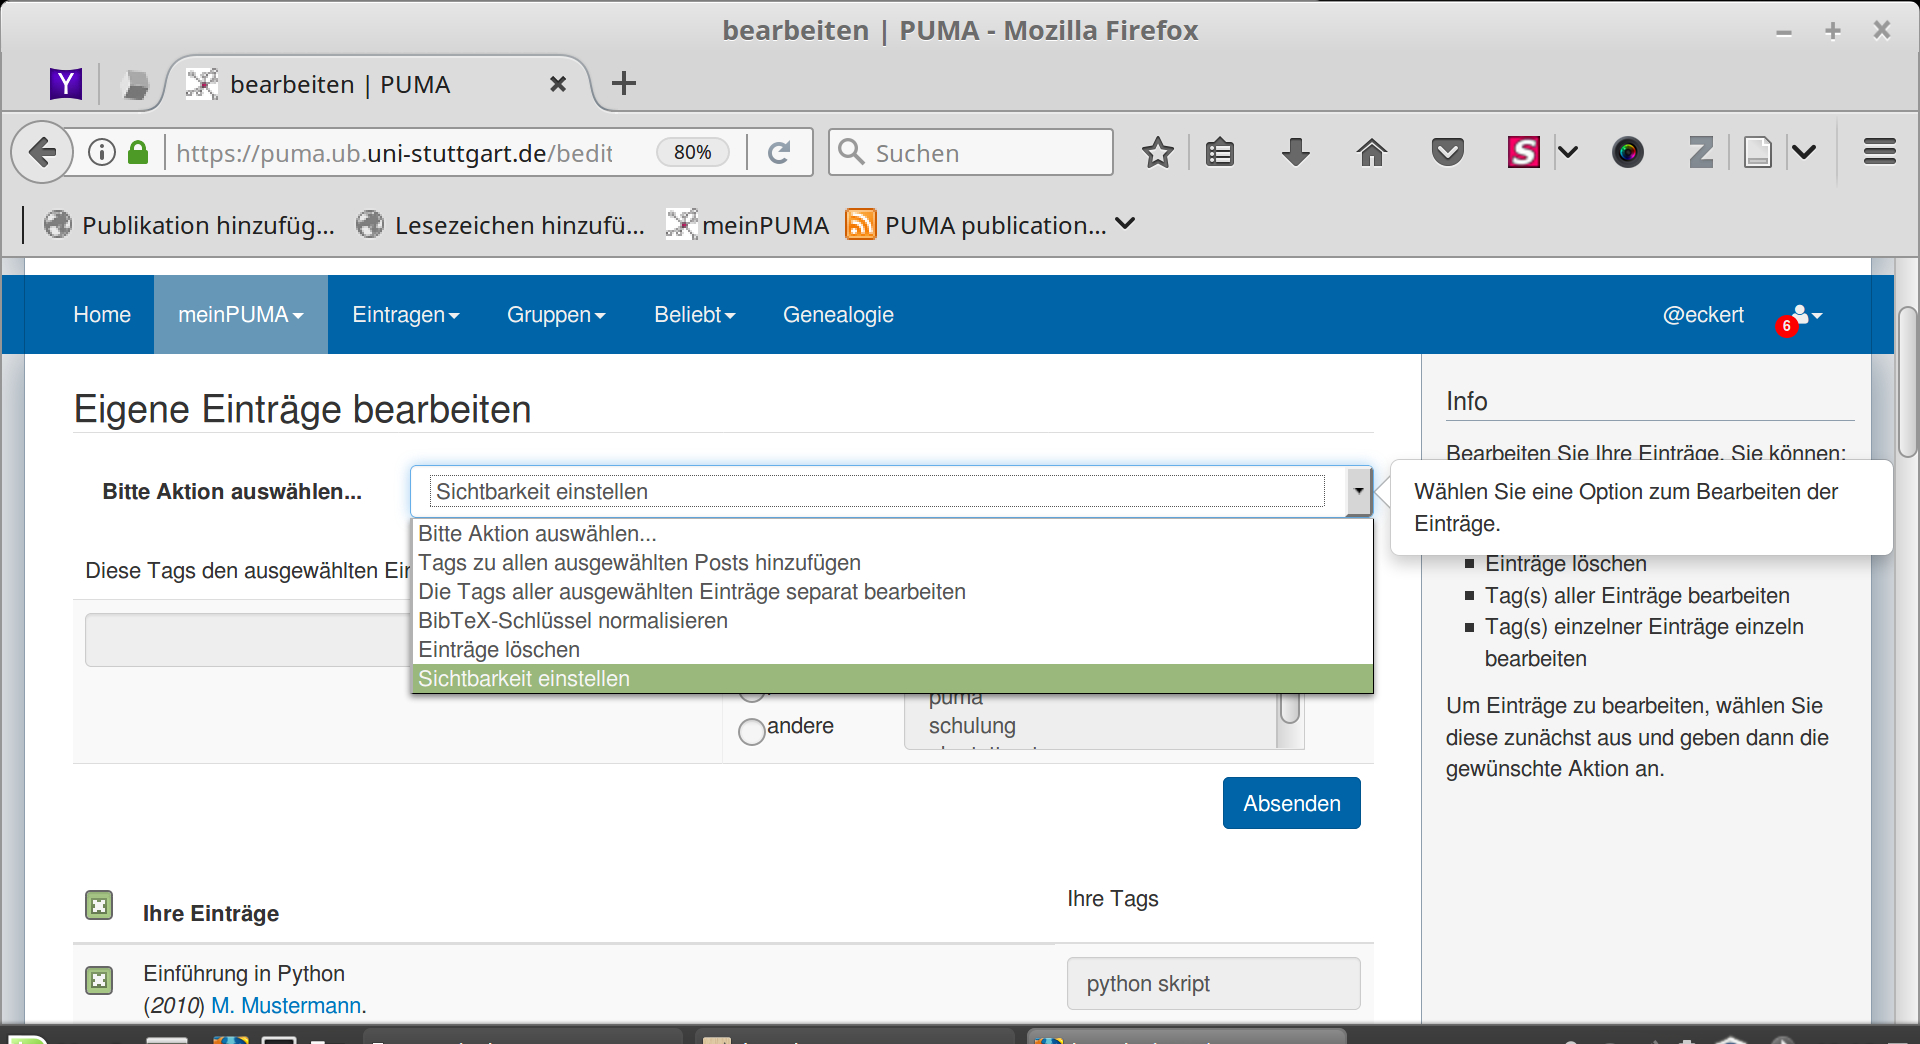
\includegraphics[width=10cm]{Bilder/Kapitel6/Eigene_Eintraege_bearbeiten}}
 \caption{Eigene Einträge bearbeiten}
 \label{figure030}
\end{figure}
\subsection{Open-URL Resolver/Bestandsanfrage}
Mit Hilfe von Open-URL\index{Open-URL} kann man bei Publikationen aus seiner eigenen Sammlung überprüfen, ob sich diese im Katalog der jeweiligen Büchereien befindet. Dafür müssen Sie  die folgende URL:  
\url{http://www.redi-bw.de/links/unist} in Ihre Einstellungen kopieren, dabei gehen Sie wie folgt vor:
\begin{enumerate}
    \item Klicken Sie auf das Personensymbol, ein Untermenü öffnet sich.
    \item Klicken Sie auf \enquote{Einstellungen}.
    \item Geben Sie in der Rubrik \enquote{Kontakt} in das Feld \enquote{OpenURL} die URL \url{http://www.redi-bw.de/links/unist} ein. 
\begin{figure}[h!]
 \centering
 \fbox{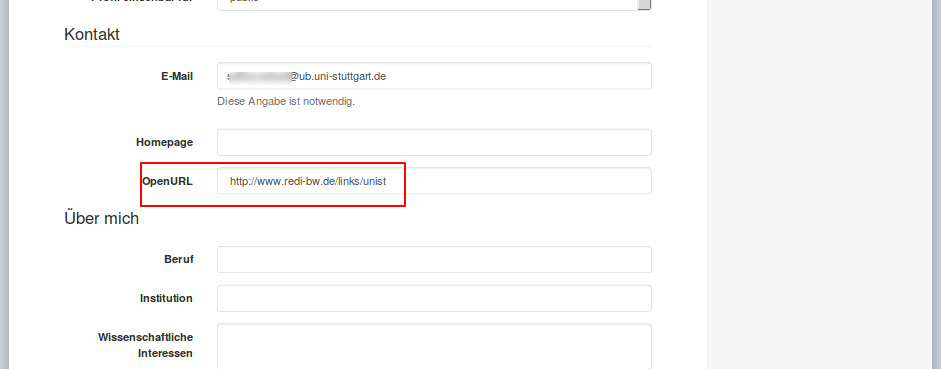
\includegraphics[width=10cm]{Bilder/Kapitel6/Open_URL}}
 \caption{Open-URL der Universität Stuttgart}
 \label{figure031}
\end{figure}
    \item Speichern Sie die Änderung auf dem Ende der Seite.
\end{enumerate}
Ab sofort befindet sich bei jeder Ihrer Publikationen unter dem Bereich \enquote{Links und Ressourcen} die entsprechende Open-URL, über die Sie nun eine Bestandsabfrage durchführen können.
\begin{figure}[h!]
 \centering
 \fbox{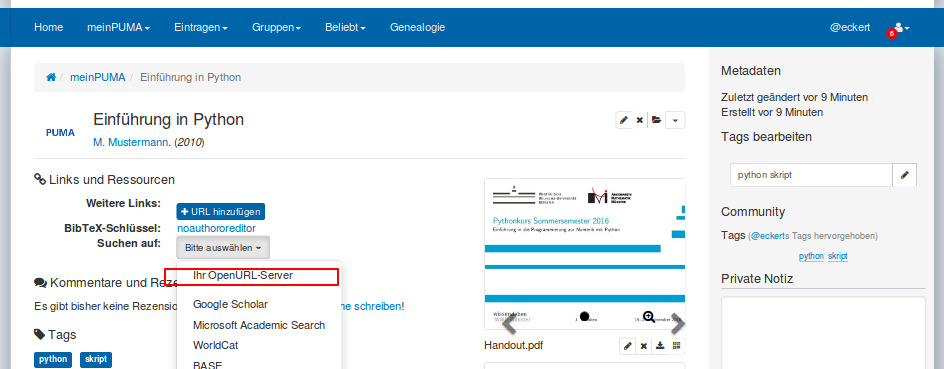
\includegraphics[width=10cm]{Bilder/Kapitel6/OpenURL-Resolver}}
 \caption{OpenURL-Resolver}
 \label{figure032}
\end{figure}
\subsection{Open Access-Zugriff auf Publikationsdienste}%Screenshot
Der Zugriff auf Open Access\index{Open Access} Publikationsdienste ermöglicht Ihnen über die Detailansicht einer Publikation nach der digitalen Ausgabe in einer Open Access-Datenbank zu suchen. Voraussetzung hierfür ist, dass die Detailansicht der Publikation aufgerufen ist. Zur Detailansicht gelangen Sie, indem Sie im Inhaltsbereich oder Ihrer persönlichen Sammlung (unter \enquote{Mein PUMA}) auf den Titel einer Publikation klicken. 
\begin{enumerate}
    \item Klicken Sie auf das Auswahlmenü \enquote{Suchen auf}. Ein Untermenü erscheint.
\begin{figure}[h!]
 \centering
 \fbox{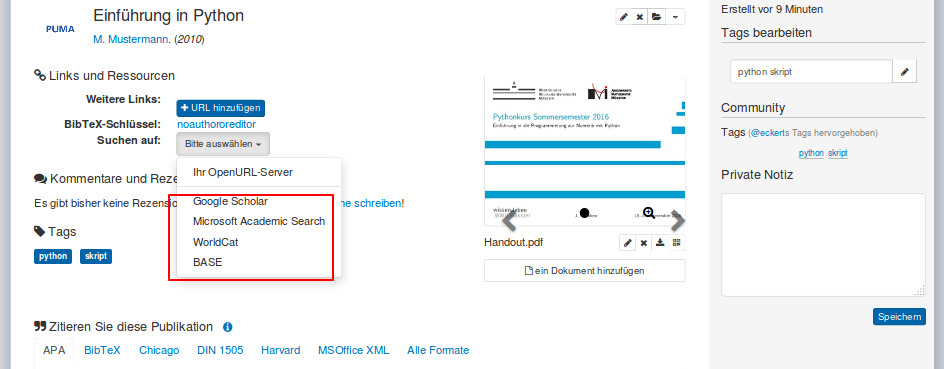
\includegraphics[width=10cm]{Bilder/Kapitel6/Open-Access}}
 \caption{Open Access}
 \label{figure033}
\end{figure}
    \item Wählen Sie aus der angezeigten Liste die Open Access-Datenbank, die Sie nach diesem Artikel durchsuchen möchten. 
\end{enumerate}
 So gelangen Sie schnell und einfach zu der digitalen Ausgabe einer Publikation. 
\subsection{Eingang}
In Ihrem Eingang\index{Eingang} finden Sie alle Beträge, die Ihnen von Freunden geschickt wurden.
\begin{figure}[h!]
 \centering
 \fbox{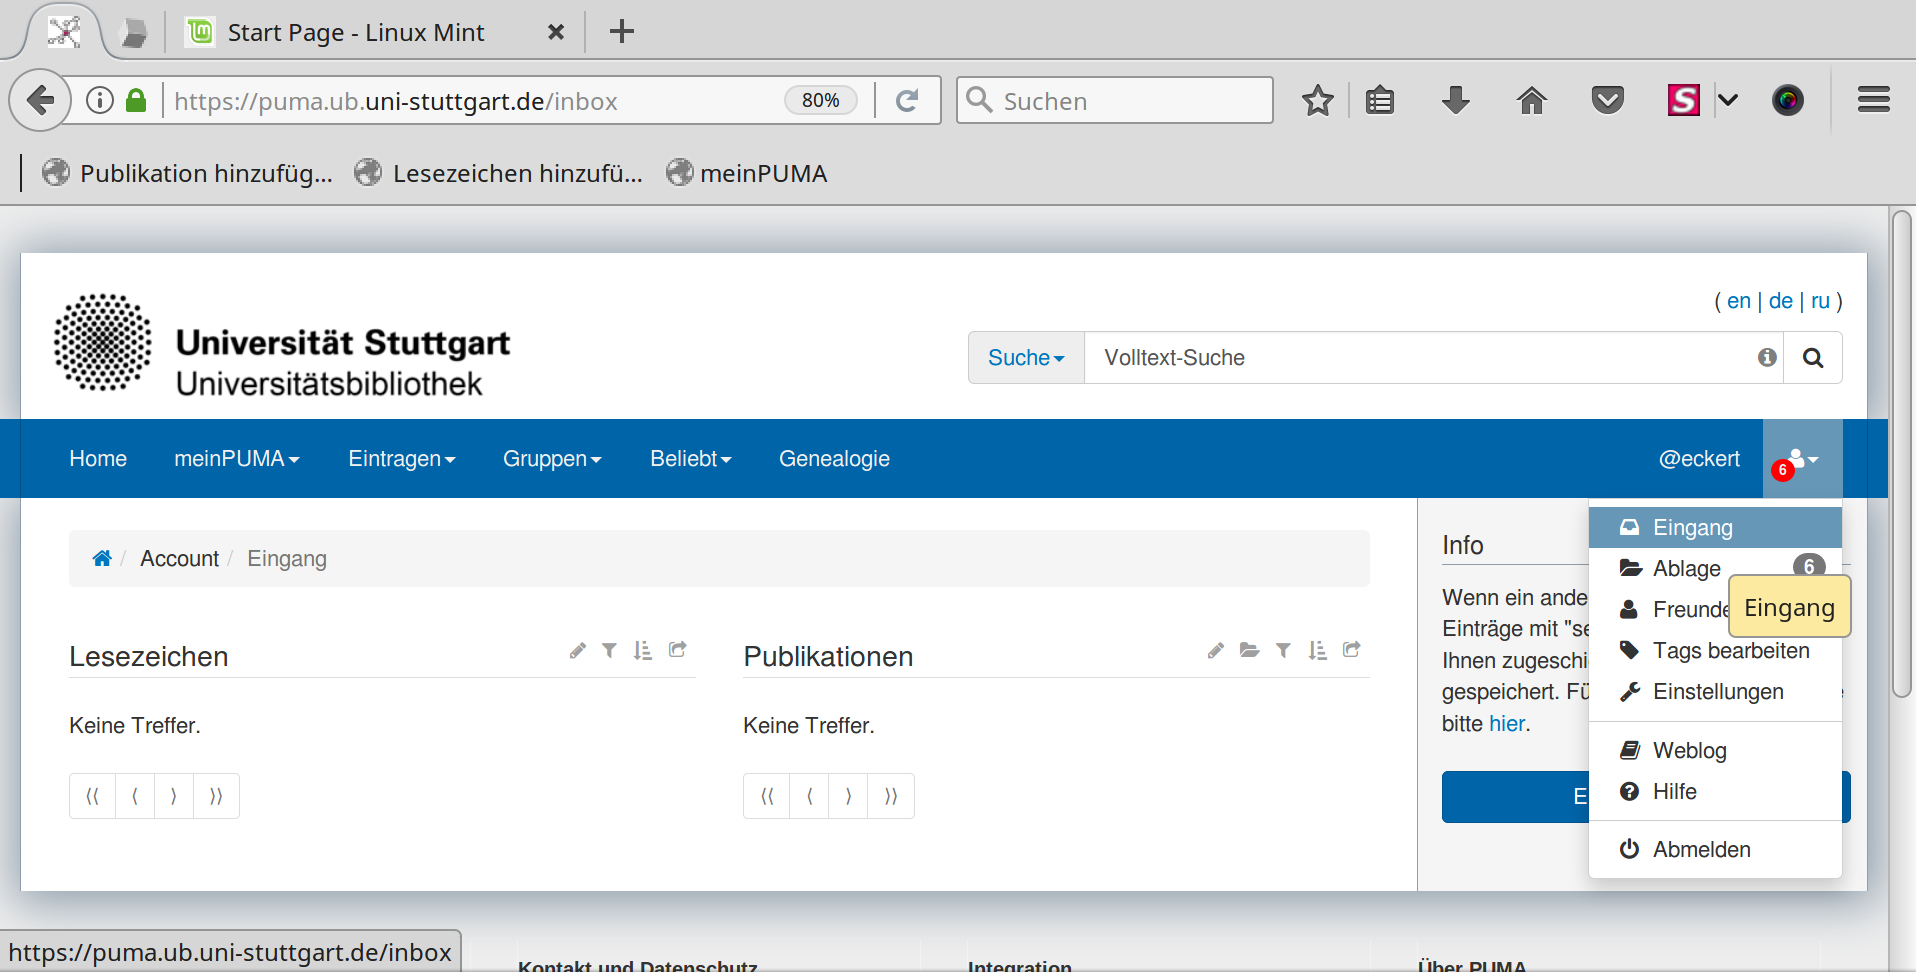
\includegraphics[width=10cm]{Bilder/Kapitel6/Eingang}}
 \caption{Der Eingang}
 \label{figure034}
\end{figure}
\underline{Einträge verschicken\index{Einträge!verschicken}}
\newline
Um einem anderen Nutzer ein Lesezeichen oder eine Publikation zu schicken, verwenden Sie das Systemtag \textit{send:xyz}. Dieses Tag geben Sie mit weiteren Tags beim Eintragen einer Publikation/Lesezeichen mit ein. Der Eintrag wird dann getaggt mit from:<YourUserName> und in den Eingang von dem Nutzer xyz kopiert. Um den Missbrauch des Eingangs zu verhindern, muss der Empfänger des Eintrags
\begin{enumerate}
    \item entweder mit Ihnen befreundet sein
    \item oder Mitglied einer gemeinsamen Gruppe sein.
\end{enumerate}
Nachdem der Eintrag gesendet wurde wird der Tag von \textit{send:xyz} in \textit{sent:xyz} automatisch umgewandelt.
\newline
\newline
\underline{Einträge erhalten\index{Einträge!erhalten}}
\newline
In Ihrem Eingang liegen alle Einträge, die Ihnen geschickt wurden. Sie können diese Einträge über den Button \enquote{Diese Publikation in die eigene Sammlung einfügen}, rechts neben dem Eintrag (zwei Blätter) übernehmen. Mit \enquote{Diese Publikation aus Ihrem Eingang entfernen} können Sie den Eintrag aus dem Eingang löschen und über das schwarze Zahnrad den ganzen Eingang leeren.
\section{Literaturlisten erstellen}
PUMA bietet Ihnen die Möglichkeit, aus Ihren gesammelten Publikationen Literaturlisten\index{Literaturlisten} zu erstellen, die Sie später beispielsweise auf externen Webseiten verwenden können. \newline
Hierfür fügen Sie die Publikationen, die in das Literaturverzeichnis sollen, zu Ihrer Ablage\index{Ablage} hinzu. Wenn Sie alle Publikationen hinzugefügt haben, klicken Sie in der Ablage, oberhalb von den Publikationen, auf Exportzeichen und wählen Sie \enquote{mehr...} aus. Sie gelangen nun zu einer Übersichtsseite, auf der Ihnen alle verfügbaren Zitationsstile angezeigt werden, und Sie nur noch den passenden aussuchen müssen. 
\subsection{Eigene Literaturlisten erstellen} 
Neben den Layouts für das Erstellen einer Literaturliste können Sie auch folgenden URLs verwenden, die Sie in Ihren Browser eingeben:
\begin{enumerate}%Beispielscreenshots ?
    \item \textbf{Allgemeine Liste:}\newline
    \textit{https://puma.ub.uni-stuttgart.de/publ/user/<username>} \newline
    Ersetzen Sie \textit{<username>} durch Ihren Benutzernamen und Ihnen werden alle Publikationen aus Ihrer Sammlung in einer Literaturliste angezeigt.\newline
    \textbf{Beispiel:} https://puma.ub.uni-stuttgart.de/publ/user/eckert 
\begin{figure}[h!]
 \centering
 \fbox{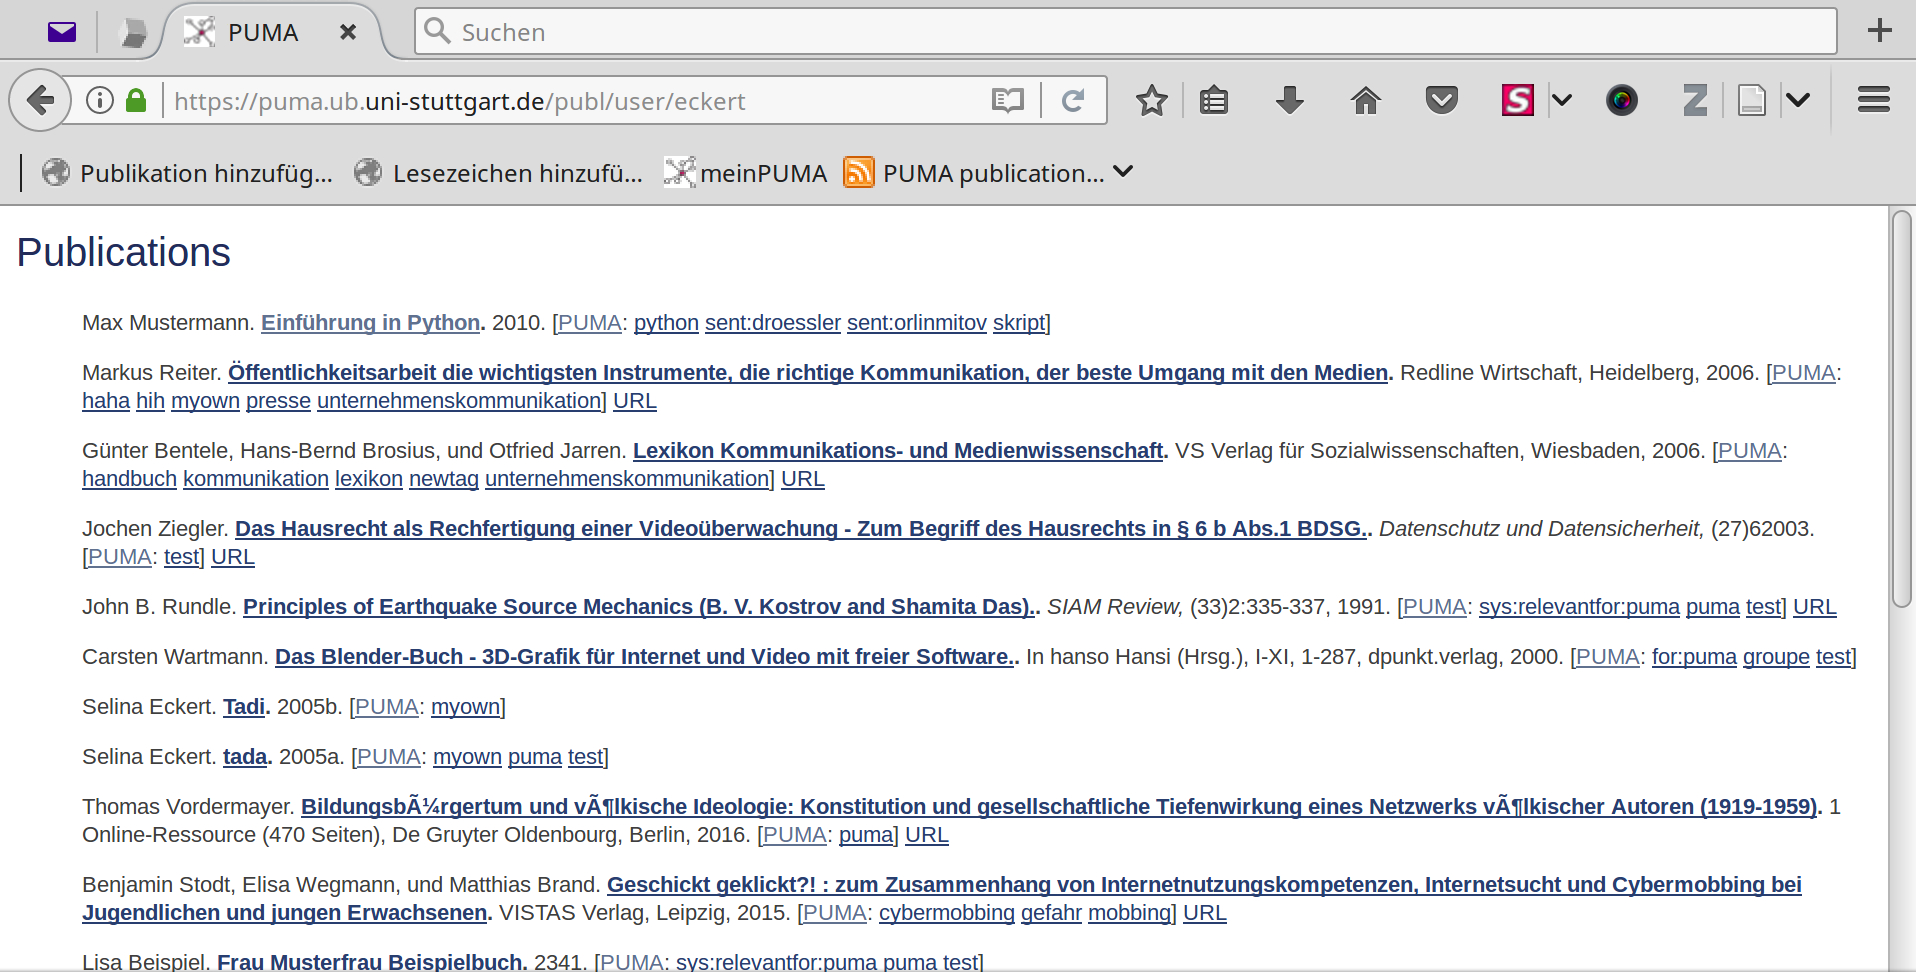
\includegraphics[width=11cm]{Bilder/Kapitel6/Allgemeine_Liste}}
 \caption{Allgemeine Liste}
 \label{figure035}
\end{figure}

    \item \textbf{Allgemeine Liste ohne Tags:}\newline
    \textit{https://puma.ub.uni-stuttgart.de/publ/user/<username>?notags=1}\newline
    Ersetzen Sie \textit{<username>} durch Ihren Benutzernamen und Ihnen werden alle Publikationen aus Ihrer Sammlung, ohne Tags, in einer Literaturliste angezeigt.\newline
    \textbf{Beispiel:} https://puma.ub.uni-stuttgart.de/publ/user/eckert?notags=1 
    
\begin{figure}[h!]
 \centering
 \fbox{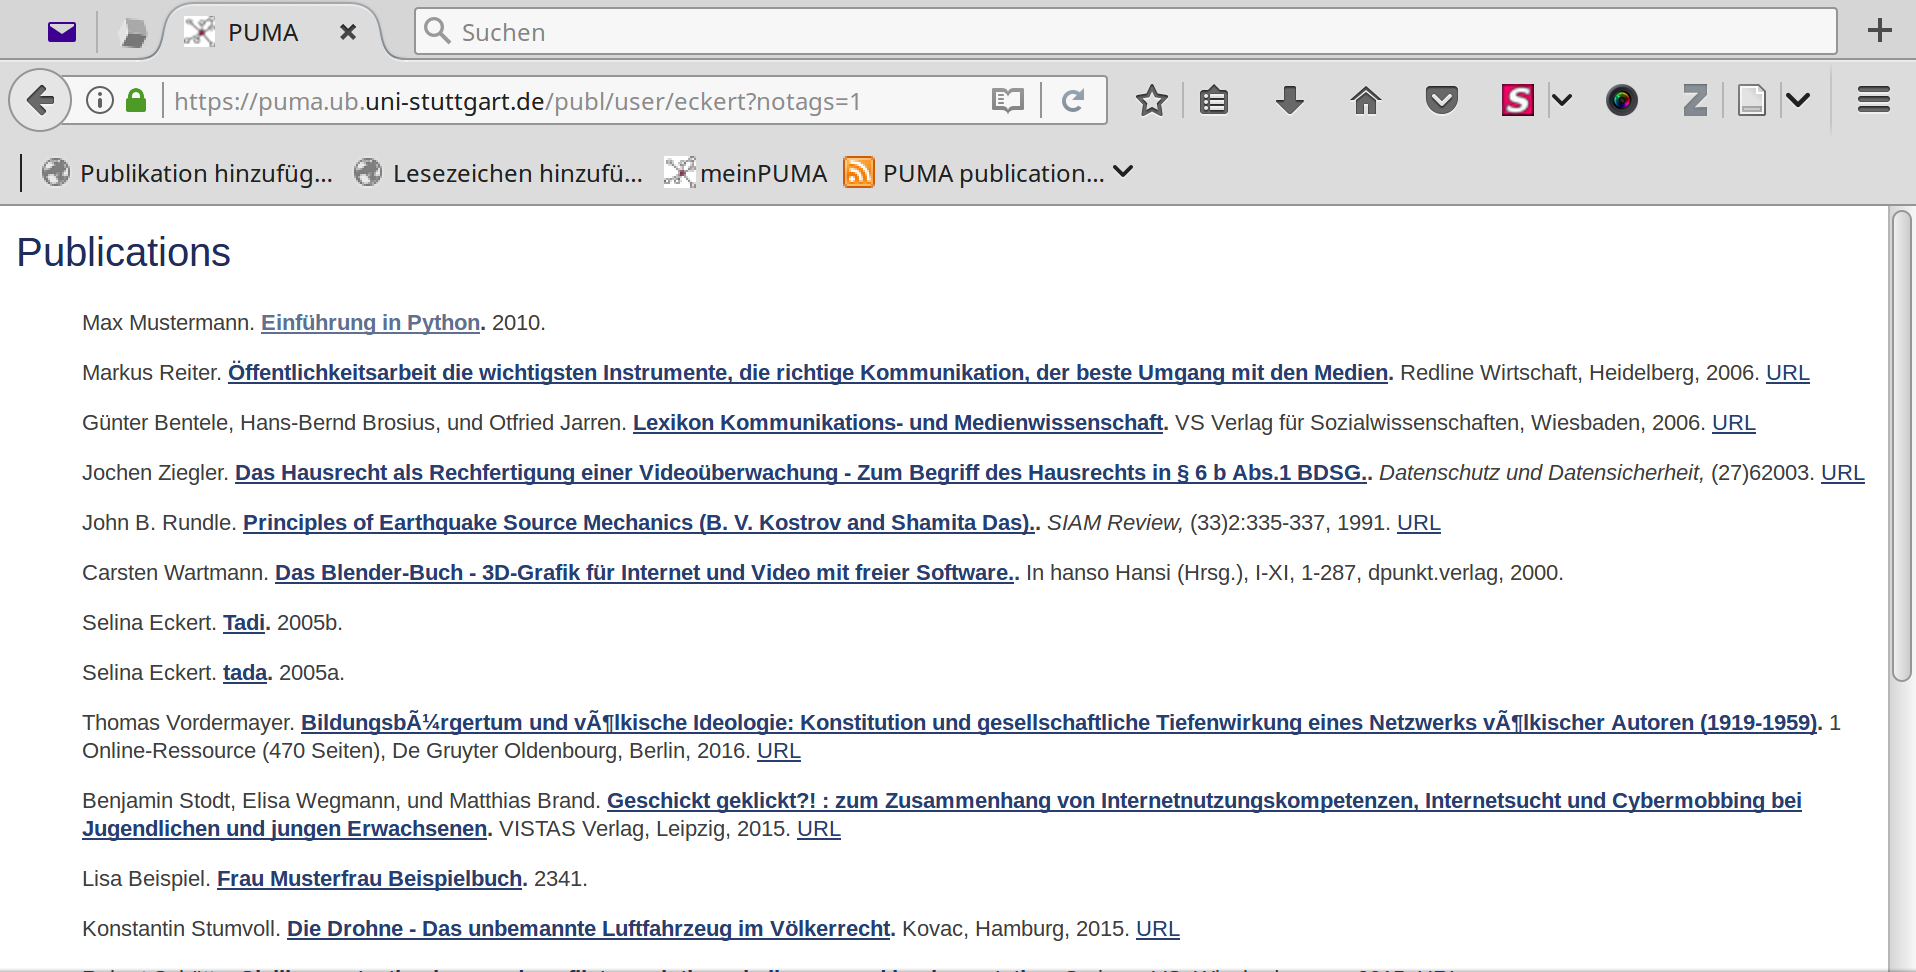
\includegraphics[width=11cm]{Bilder/Kapitel6/Allgemeine_Liste_ohne_Tags}}
 \caption{Allgemeine Liste ohne Tags}
 \label{figure036}
\end{figure}

    \item \textbf{Allgemeine Liste mit Tag-Einschränkung:}\newline
    \textit{https://puma.ub.uni-stuttgart.de/publ/user/<username>/<tagname>}\newline
    Ersetzen Sie \textit{<username>} durch Ihren Benutzernamen und \textit{<tagname>} durch den Tag, der in den Publikationen enthalten sein soll. Ihnen wird eine Literaturliste angezeigt, die jene Publikationen aus Ihrer Sammlung enthält, die den speziellen Tag enthalten. Ein besonderes Beispiel hierfür ist der Tag \textit{myown\index{myown}}. Durch diesen Tag geben Sie an, dass Sie der/~die Verfasser/~in der Publikation sind. \newline
    \textbf{Beispiel:} https://puma.ub.uni-stuttgart.de/publ/user/eckert/puma
   
\begin{figure}[h!]
 \centering
 \fbox{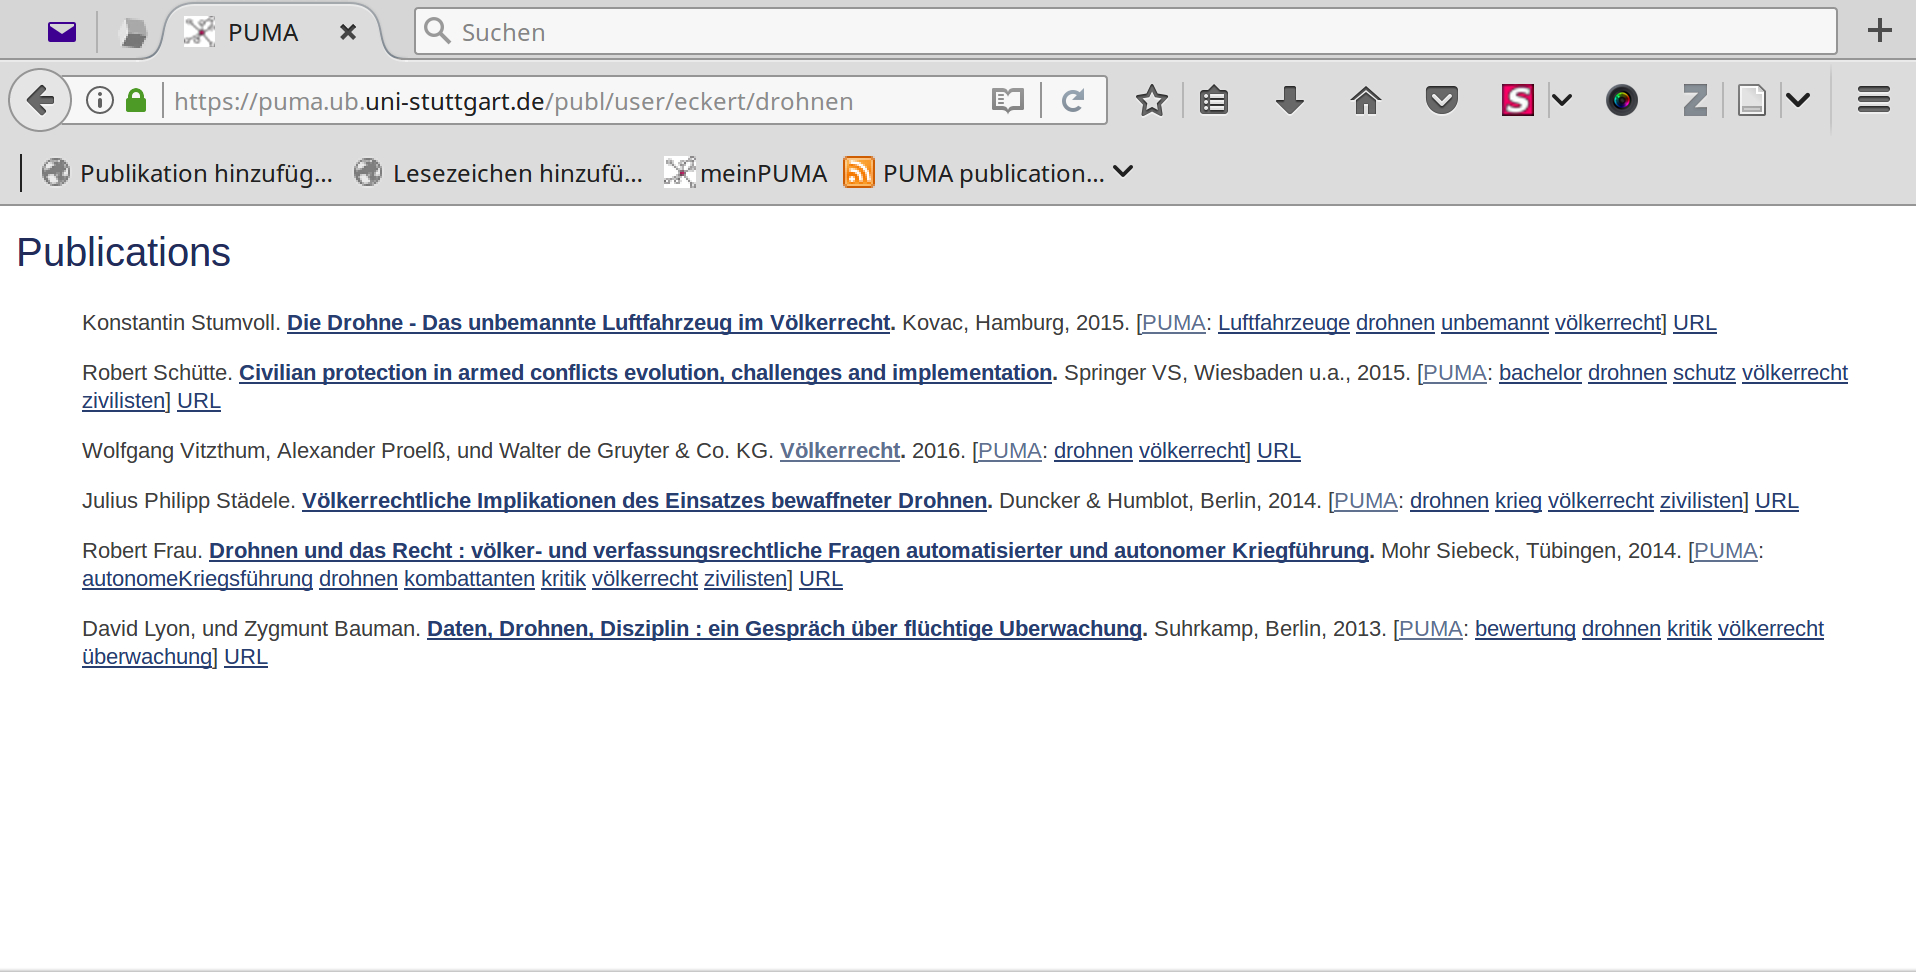
\includegraphics[width=11cm]{Bilder/Kapitel6/Allgemeine_Liste_Tag_Einschraenkung}}
 \caption{Liste mit Tagauswahl}
 \label{figure037}
\end{figure}

    \item \textbf{BibTeX-Liste:}\newline
    \textit{https://puma.ub.uni-stuttgart.de/bib/user/<username>} \newline
    Ersetzen Sie \textit{<username>} durch Ihren Benutzernamen. Ihnen wird eine Literaturliste mit all Ihren Publikationen im BibTex-Format\index{BibTex} angezeigt.\newline
    \textbf{Beispiel:} https://puma.ub.uni-stuttgart.de/bib/user/eckert 

\begin{figure}[h!]
 \centering
 \fbox{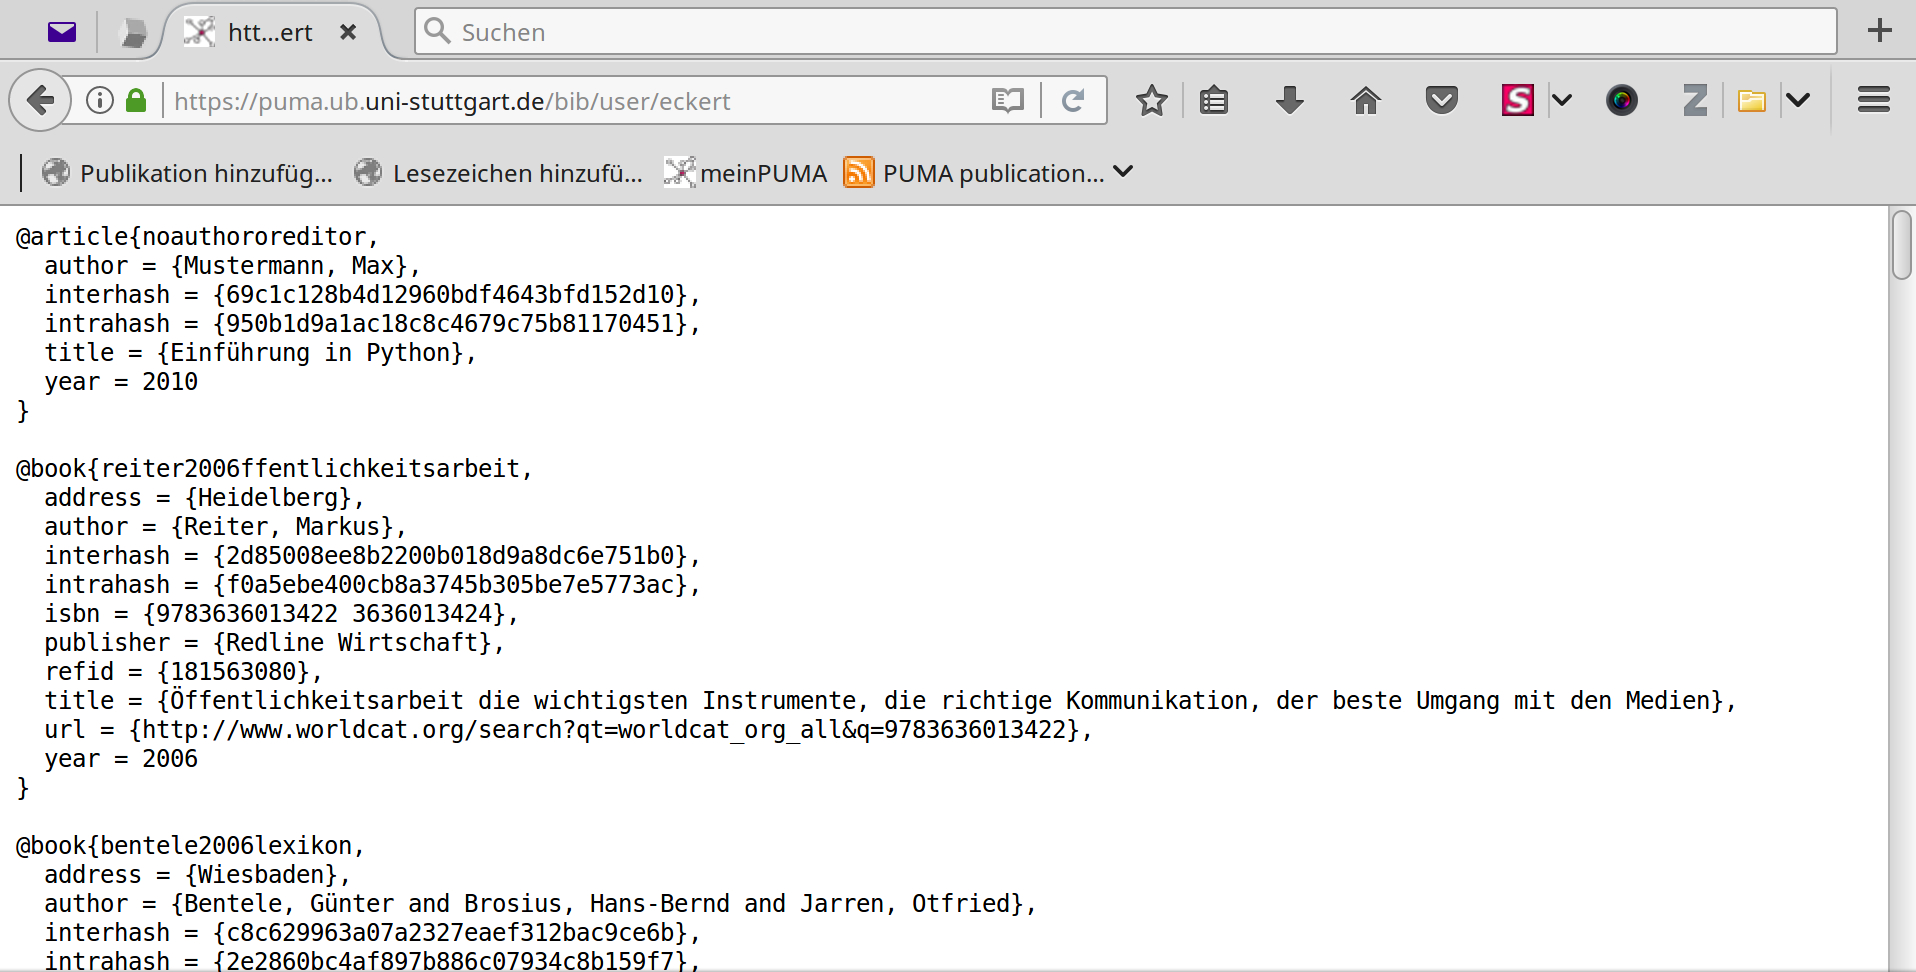
\includegraphics[width=11cm]{Bilder/Kapitel6/Bibtex_Liste}}
 \caption{BibTex-Liste}
 \label{figure038}
\end{figure}

\end{enumerate}
\subsection{JabRef-Layouts}
Einen kompletten Überblick zu allen verfügbaren Jabref-Layouts\index{JabRef!Layouts} erhalten Sie auf der Export-Seite von PUMA.
\begin{enumerate}
	\item  \textbf{/layout/simplehtml/}\newline
	Sie erhalten eine HTML-Übersicht - über alle Publikationen im 		Inhaltsbereich - ohne Kopf- oder Fußzeile nützlich für die 			Einbindung von Publikationslisten in andere HTML-Seiten.
	\item \textbf{/layout/html/}\newline
    Eine einfache Übersicht aller Publikationen aus dem Inhaltsbereich, in der jeder Eintrag als Zeile in einer Tabelle dargestellt ist.
	\item \textbf{/layout/tablerefs/} \newline
    HTML-Ausgabe mit jedem Eintrag als Zeile in einer Tabelle und einer zusätzlichen JavaScript-Suchfunktion.
\item \textbf{/layout/tablerefsabsbib/} \newline
    Ähnelt \textit{/layout/tablerefs/}. Enthält auch die BibTeX-Quelle und die Kurzbeschreibung der Publikation.
\item \textbf{/layout/docbook/} \newline
    Dies ist eine XML-Ausgabe gemäß dem DocBook-Schema.
\item \textbf{/layout/endnote/} \newline
    Sie erhalten eine Ausgabe in RIS, welche von dem Literaturverwaltungsprogramm EndNote verwendet wird.
\item \textbf{/layout/dblp/} \newline
    DBLP exportiert alle Publikationen aus dem Inhaltsbereich in eine DBLP-konforme XML-Struktur. 
\item \textbf{/layout/text/}\newline
    Alle Publikationen aus dem Inhaltsbereich werden in einer BibTeX-Ausgabe dargestellt.
\end{enumerate}



\chapter{Export und Import}
\label{ch:exportImport}
\textit{Nicht nur in der Wirtschaft spielen Import und Export eine wichtige Rolle. Auch PUMA ist global vernetzbar.}
\section{Literaturlisten exportieren}
\label{sec:llExportieren}
PUMA ermöglicht den vollständigen Export\index{Export} von Publikationslisten aus PUMA in andere Programme. Das gängigste Datenformat, dass die meisten Programme unterstützen, ist BibTex\index{BibTex}. \newline 
Der Export erfolgt in zwei Schritten. Es wird zuerst ein Literaturverzeichnis in Puma zusammengestellt und exportiert, bevor es dann in das andere Programm importiert wird.
\subsection{Literaturverzeichnis zusammenstellen}
\label{subsec:lvZusammenstellen}
\begin{enumerate}
    \item Um ein Literaturverzeichnis zusammenzustellen, müssen Sie im ersten Schritt die Publikationen, die in Ihrem Verzeichnis abgelegt werden sollen, in Ihre Ablage\index{Ablage} kopieren. Hierfür gehen Sie in Ihre persönliche Publikations- und Lesezeichensammlung über den @Ihr Benutzername-Button oder klicken im Dropdown-Menü von \enquote{meinPUMA} auf \enquote{meine Einträge}.  Neben jeder Publikation befindet sich eine Symbolleiste.
    \item Klicken Sie auf das Aktenordner-Symbol (\enquote{Diese Publikation zur Ablage hinzufügen}). Die Publikation gelangt nun automatisch in Ihre Ablage und wird dort gespeichert.
\begin{figure}[h!]
 \centering
 \fbox{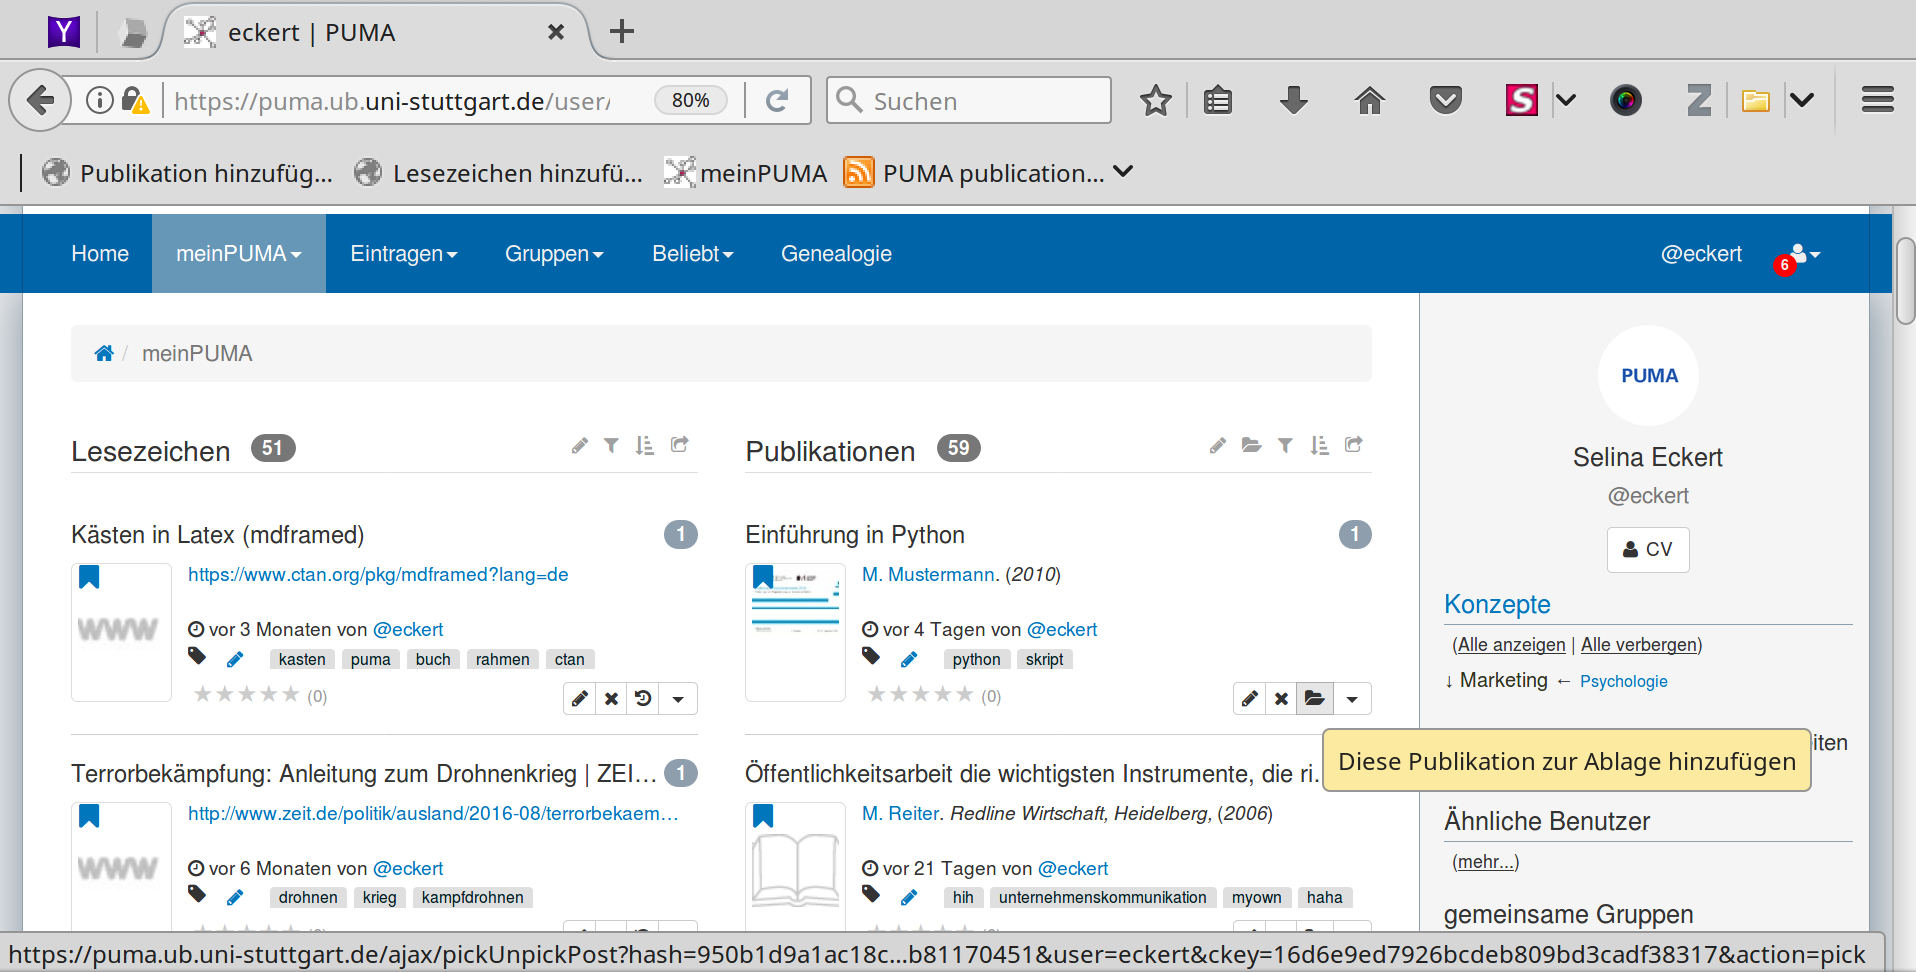
\includegraphics[width=10cm]{Bilder/Kapitel7/Zur_Ablage_hinzufuegen}}
 \caption{Zur Ablage hinzufügen}
 \label{fig:zurAblageHinzu}
\end{figure}
    \item Zur Ablage gelangen Sie über das Personensymbol. Klicken Sie im Dropdown-Menü auf \enquote{Ablage} und Ihnen werden alle Publikationen, die sich in Ihrer Ablage befinden angezeigt. 
\end{enumerate} 
Schnellerer Weg: Klicken Sie auf das Einstellungs-Zahnrad im Inhaltsbereich über den Publikationen. Wählen Sie unter der Rubrik \enquote{Ablage} \enquote{alle hinzufügen} aus. Alle Publikationen aus dem Inhaltsbereich werden in die Ablage übernommen. 
\subsection{Literaturverzeichnis exportieren}
\label{subsec:lvExportieren}
\textbf{Voraussetzung:} Sie haben ein Literaturverzeichnis zusammengestellt.
\begin{enumerate}
    \item Klicken Sie in der Ablage auf das Exportzeichen oben rechts. Ein Dropdown-Menü erscheint.
\begin{figure}[h!]
 \centering
 \fbox{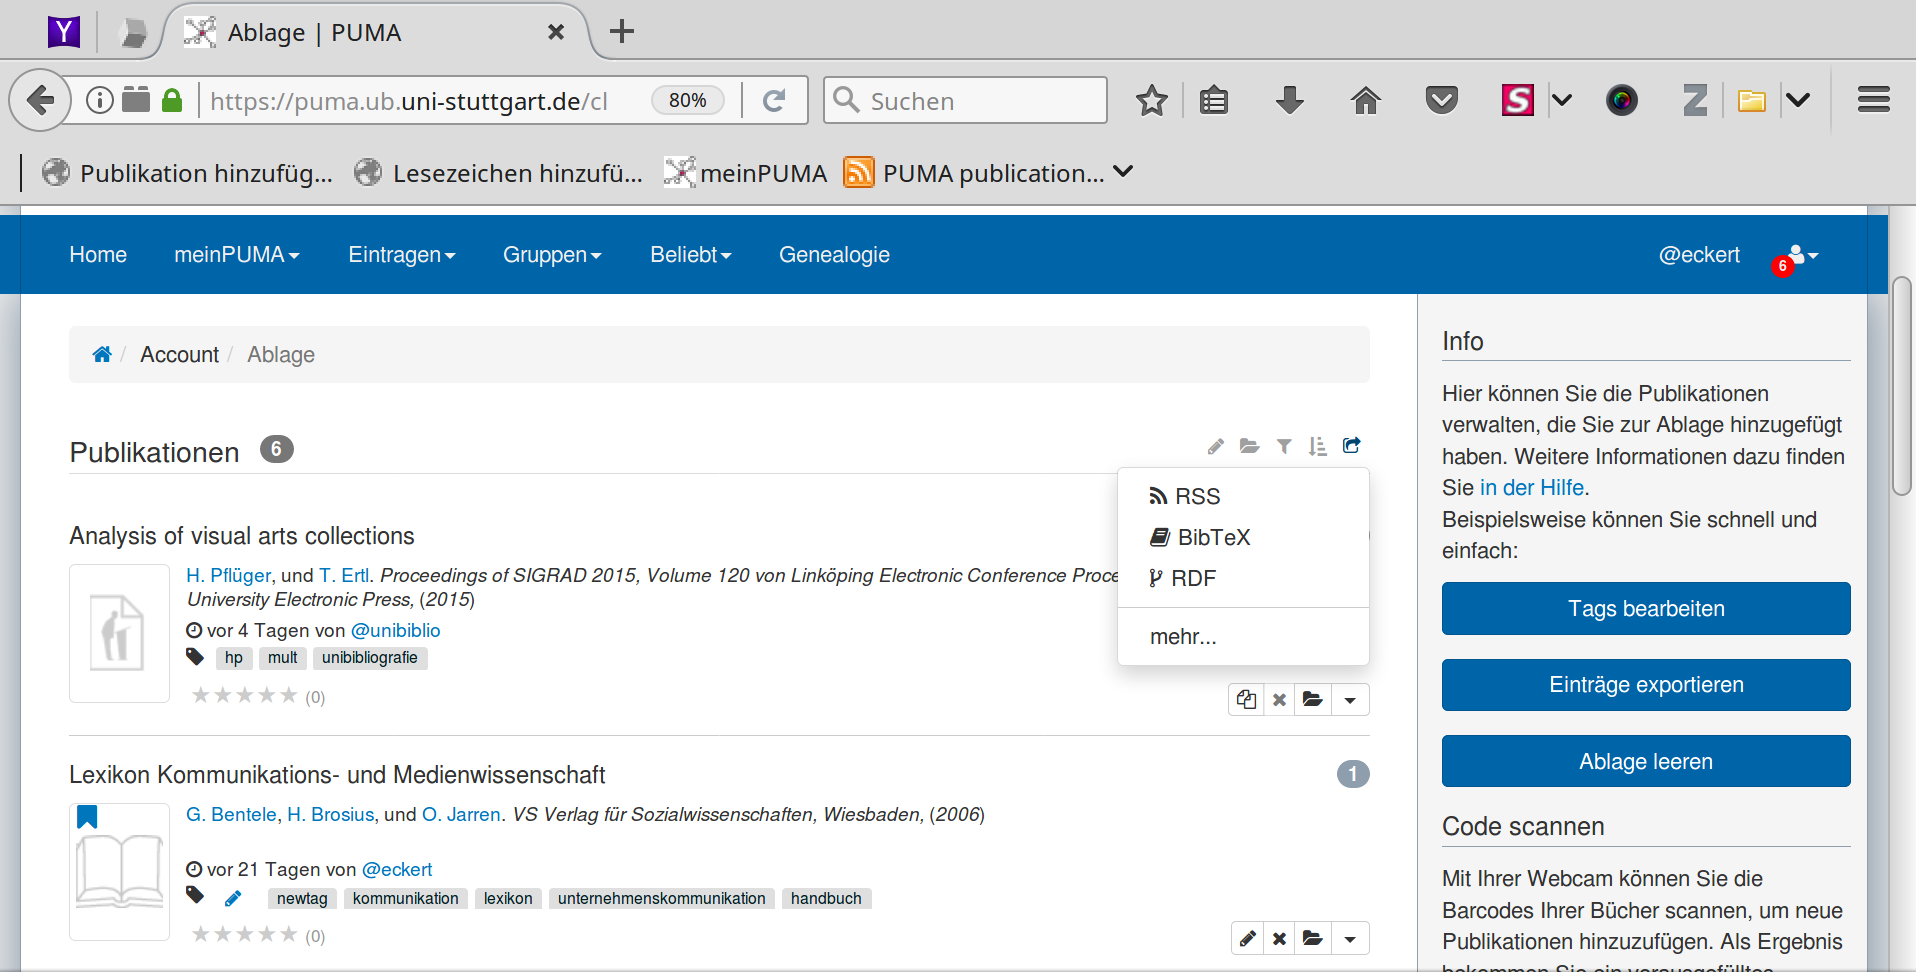
\includegraphics[width=11cm]{Bilder/Kapitel7/Exportformat_auswaehlen}}
 \caption{Das Exportformat auswählen}
 \label{fig:exportformatAuswaehlen}
\end{figure}
    \item Wählen Sie das Format, in dem Sie ihr Literaturverzeichnis haben möchten. PUMA gibt Ihnen einige Beispiele vor (RSS, BibTex, RDF). Klicken Sie auf \enquote{mehr...} haben Sie auch die Möglichkeit Ihr Literaturverzeichnis mit weiteren Formaten zu exportieren. 
\begin{figure}[h!]
 \centering
 \fbox{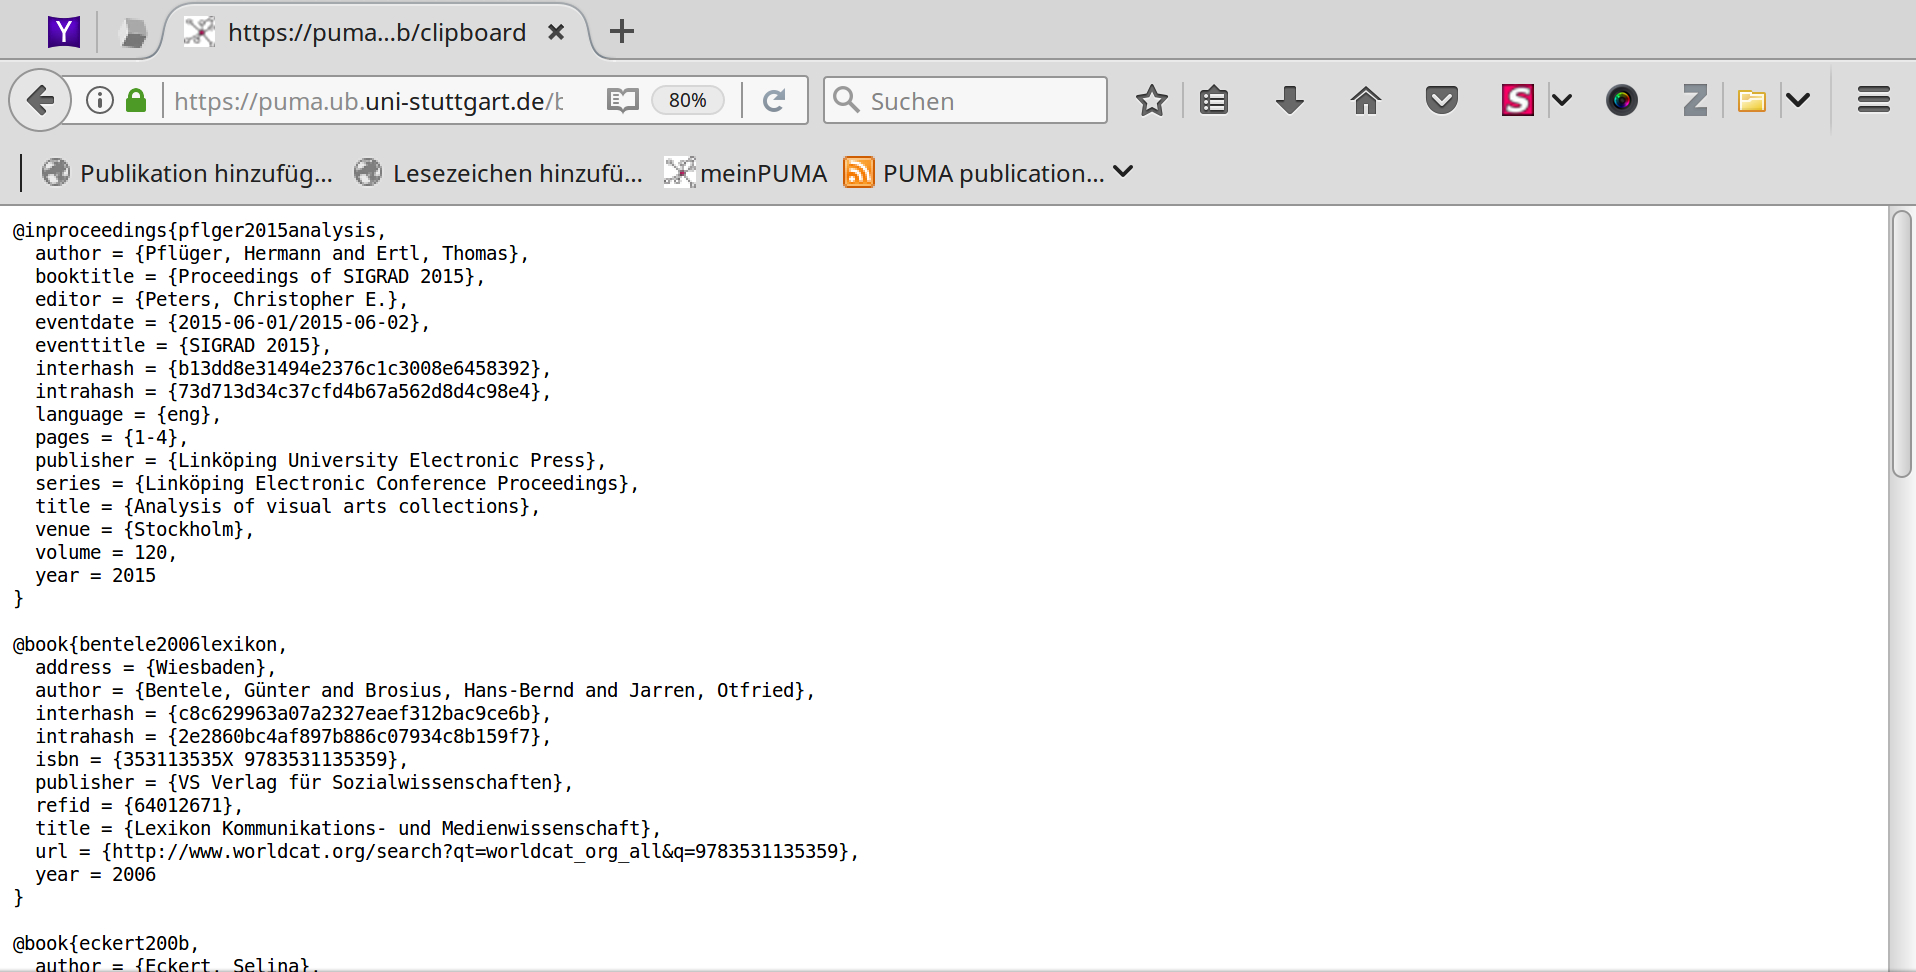
\includegraphics[width=11cm]{Bilder/Kapitel7/Das_Literaturverzeichnis}}
 \caption{Das Literaturverzeichnis}
 \label{fig:literaturverzeichnis}
\end{figure}
\begin{mdframed}[style=mdfexample1,frametitle={\texttt{TIPP}},backgroundcolor=gray!40] \texttt{Der Gebrauch des BibTex-Formates\index{BibTex} ist zu empfehlen, da dieses Format sehr verbreitet ist.}
\end{mdframed}
    \item Sobald Sie das gewählte Format angeklickt haben erscheint ein neues Fenster. Klicken Sie mit der rechten Maustaste auf die Seite und wählen \enquote{Speichern unter} um die Datei zu speichern.
\end{enumerate}
\subsection{Literaturverzeichnis exportieren- Programmspezifisch}
\label{subsec:lvExportProgramme}
\subsubsection*{Export nach Word\index{Export!Word}} \index{Word} \label{sss:exportWord}
\begin{enumerate}
    \item Klicken Sie in der Ablage auf das Exportzeichen.
    \item Wählen Sie im Dropdown-Menü \enquote{mehr...} aus.
    \item Es öffnet sich die Übersichtsseite der Exportformate. Wählen Sie das Format \enquote{MSOffice XML\index{MSOffice XML}}. Speichern Sie anschließend die Datei.
\begin{figure}[h!]
 \centering
 \fbox{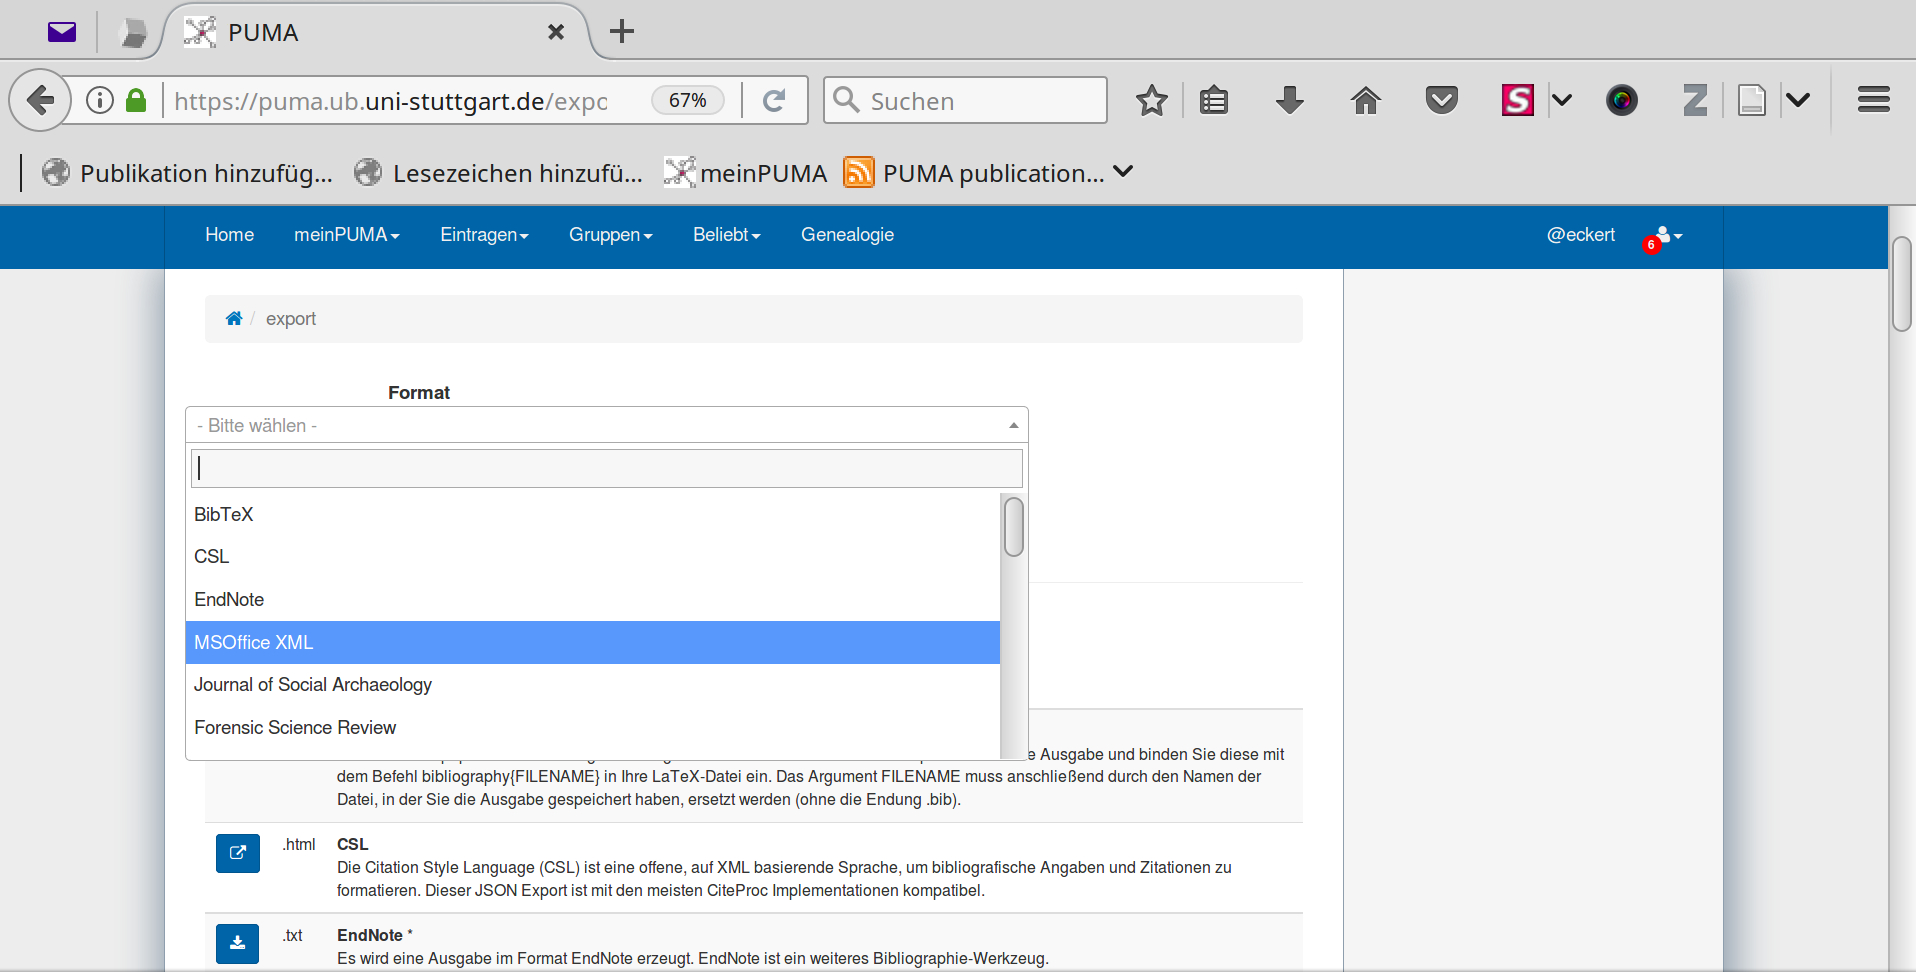
\includegraphics[width=11cm]{Bilder/Kapitel7/MSOffice_XML}}
 \caption{Das Exportformat MSOffice XML}
 \label{fig:exportformatMSOfficeXml}
\end{figure}
    \item In Microsoft Word können Sie nun die gespeicherte Datei hochladen, indem Sie unter \enquote{Verweise} auf \enquote{Quellen verwalten} klicken. Im erscheinenden Dialog (Quellen-Manager) können Sie auf \enquote{Durchsuchen} klicken und die gespeicherte Datei auswählen.
\begin{figure}[h!]
 \centering
 \fbox{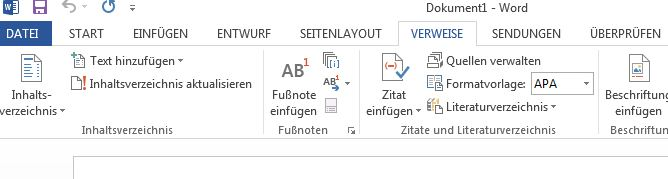
\includegraphics[width=11cm]{Bilder/Kapitel7/Word}}
 \caption{Reiter Verweise}
 \label{fig:reiterVerweise}
\end{figure}
\begin{figure}[h!]
 \centering
 \fbox{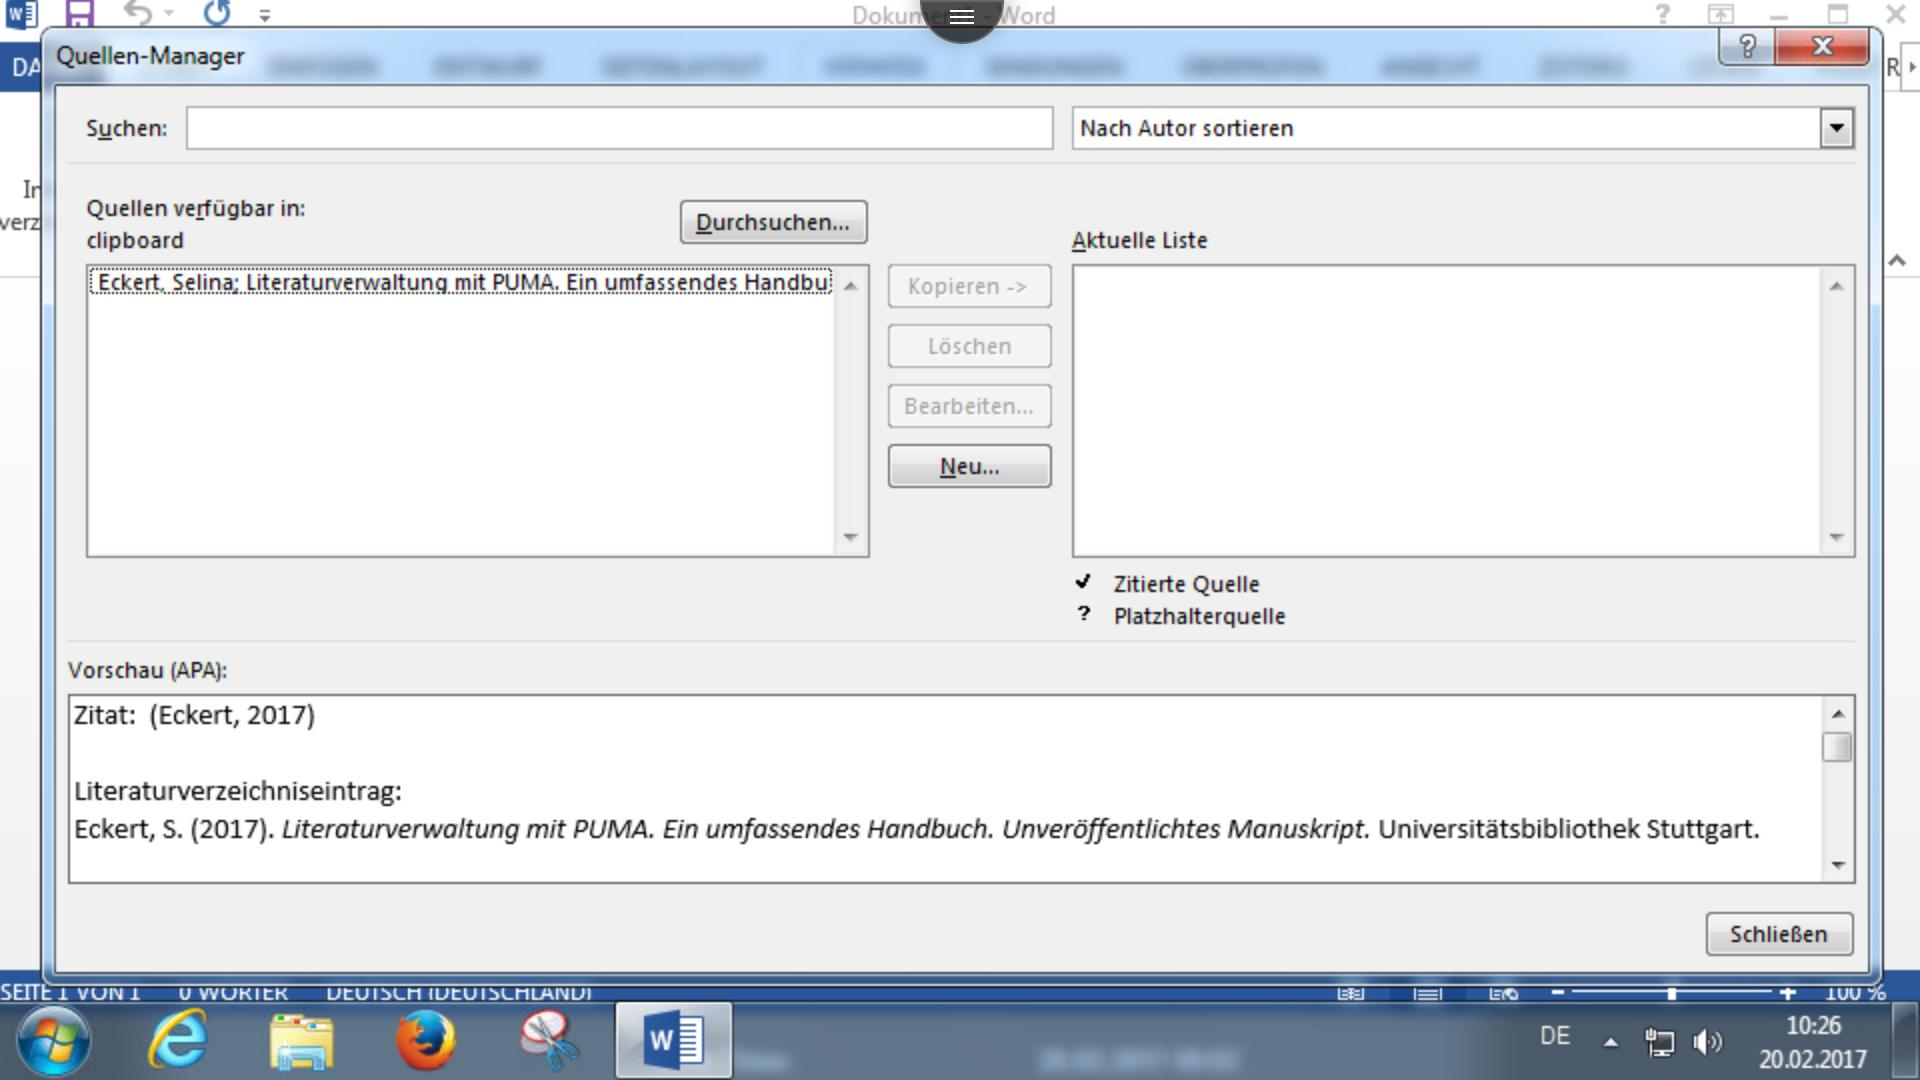
\includegraphics[width=11cm]{Bilder/Kapitel7/Quellen-Manager}}
 \caption{Quellen-Manager}
 \label{fig:quellenManager}
\end{figure} 
    \item Kopieren Sie Quellen in die aktuelle Liste, durch markieren der entsprechenden Quellen und klicken auf \enquote{Kopieren}. Schließen Sie anschließend das Fenster.
    \item Sie können sich nun das Literaturverzeichnis anzeigen lassen, indem Sie auf \enquote{Literaturverzeichnis} klicken und sich das gewünschte Layout aussuchen.
\end{enumerate}
\subsubsection*{Export nach Citavi\index{Export!Citavi}}\label{sss:exportCitavi}
\begin{enumerate}
	\item Klicken Sie auf den Titel der Publikation, die Sie nach Citavi\index{Citavi} importieren möchten.
	\item Es öffnet sich die Detailansicht der Publikation. Wählen Sie unten auf der Seite unter \enquote{Zitieren Sie diese Publikation} den Stil \enquote{BibTex\index{BibTex}} aus. 
	\item Markieren Sie die Zitation im Textfeld und kopieren Sie diese in die Zwischenablage. Benutzen Sie hierfür entweder STRG+C oder über die rechte Maustaste und \enquote{Kopieren}.
	\item Öffnen Sie Citavi. Klicken Sie in der Menüleiste oben links auf \enquote{Datei}.
	\item Wählen Sie im Dropdown-Menü \enquote{Importieren} aus. Es öffnet sich ein Popup-Fenster.
	\item Wählen Sie \enquote{Aus einer Textdatei (Ris-, BibTex-formatiert o.ä.)} aus. Klicken Sie anschließend auf \enquote{Weiter}.
	\item Wählen Sie auf der nächsten Seite BibTex als Format aus. Anschließend klicken Sie auf \enquote{Weiter}.
	\item Wählen Sie \enquote{Textdaten in der Zwischenablage verwenden} aus und klicken anschließend auf \enquote{Weiter}.
	\item Setzen Sie ein Häkchen bei \enquote{Importierte BibTex Keys ersetzen}. Klicken Sie auf \enquote{Weiter}.
	\item Wählen Sie im letzten Schritt die entsprechende Datei aus und klicken auf \enquote{Titel übernehmen}. Sie werden gefragt, ob Sie die Tags mit übernehmen möchten, setzen Sie für die Übernahmen ein Häkchen und klicken auf \enquote{OK}.
\end{enumerate}




\subsubsection*{Export nach Zotero\index{Export!Zotero}}\label{sss:exportZotero}
\begin{enumerate}
    \item Sie befinden sich auf einer PUMA-Seite (z.B. die Home-Seite oder Ihre Benutzerseite), von der Sie eine Publikation in Ihre Zotero-Bibliothek übernehmen möchten. Klicken Sie auf den schwarzen Pfeil neben dem Zotero\index{Zotero}-Symbol oben rechts bei Firefox.
    \item Ein Dropdown-Menü öffnet sich. Wählen Sie \enquote{In Zotero mit \enquote{unAPI} speichern}.
    
\begin{figure}[h!]
 \centering
 \fbox{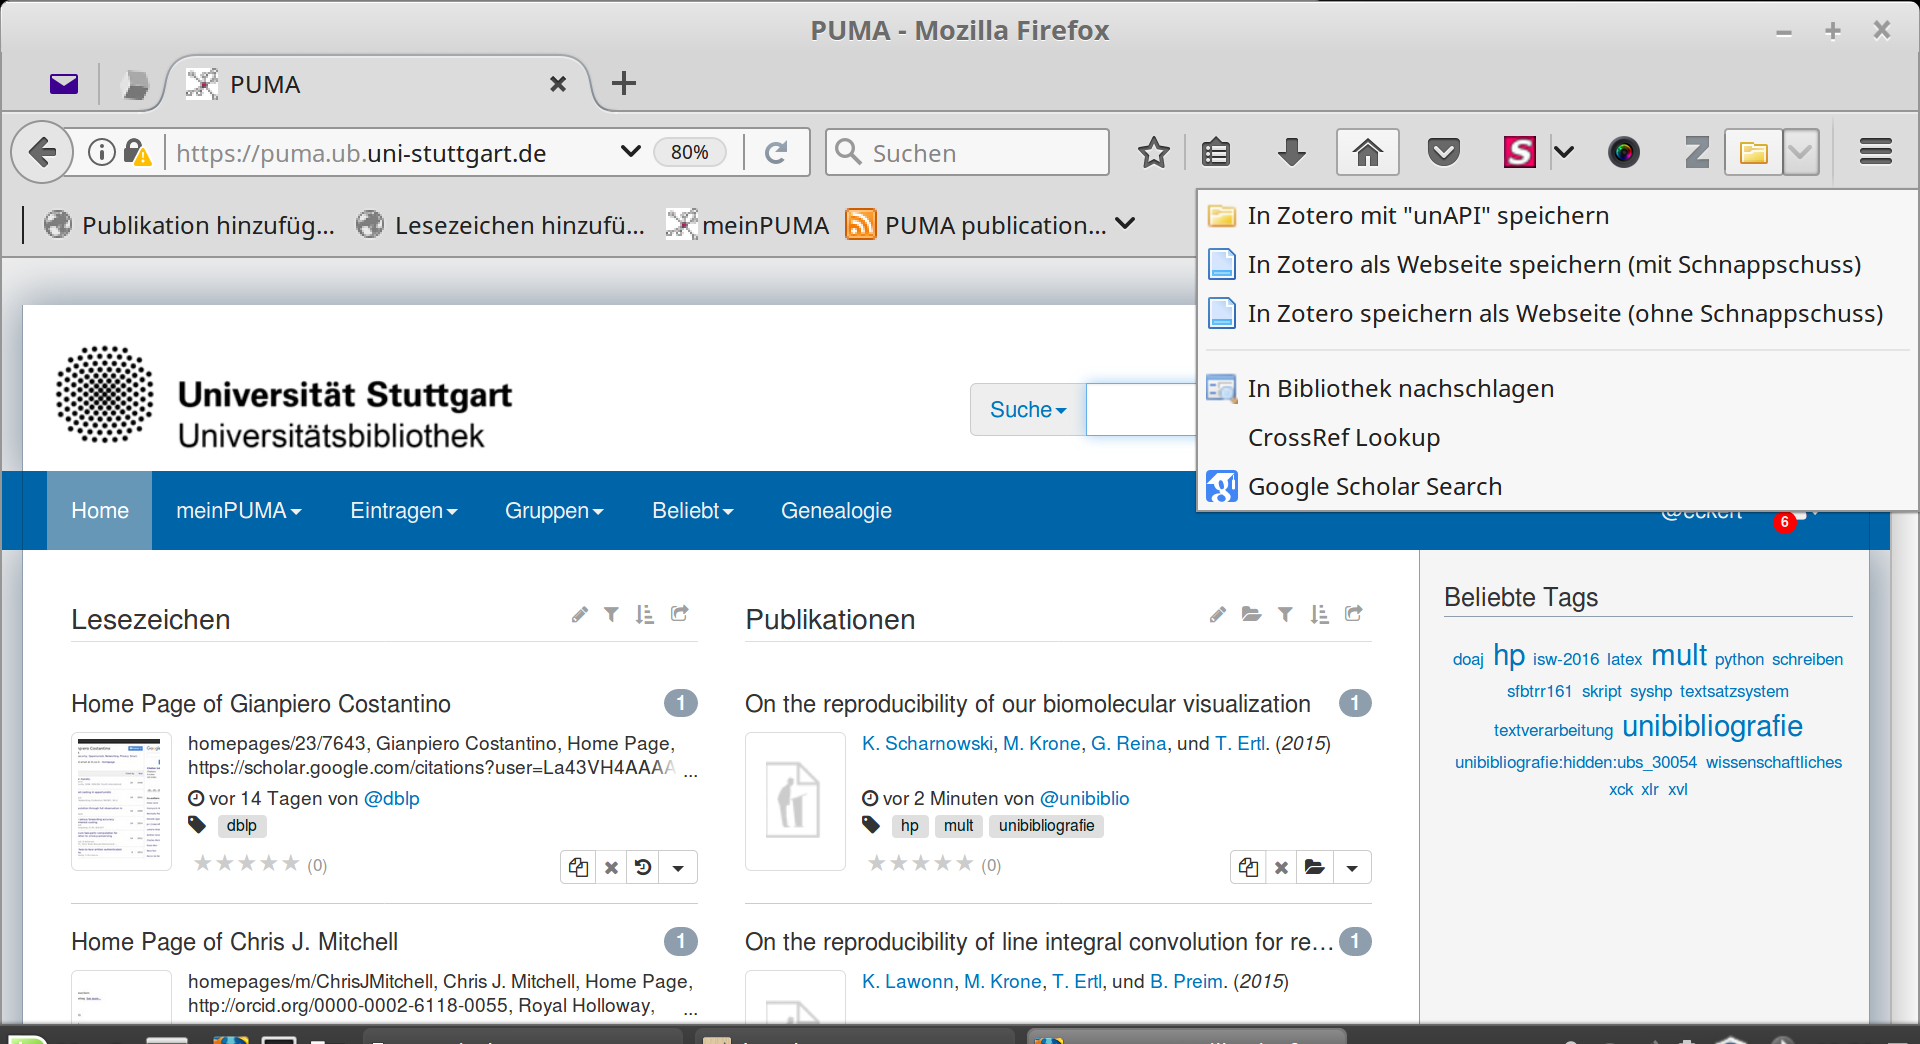
\includegraphics[width=10cm]{Bilder/Kapitel7/Zotero_Dropdown_Menue}}
 \caption{Dropdown-Menü}
 \label{fig:dropdownMenue}
\end{figure}

    \item Es öffnet sich ein Popup-Fenster, in dem alle Publikationen der entsprechenden PUMA-Seite aufgelistet sind. Wählen Sie die Publikationen aus, die Sie in Ihre Zotero-Bibliothek übernehmen möchten. Bestätigen Sie anschließend Ihre Wahl mit \enquote{OK} und Ihre ausgewählten Einträge erscheinen in Ihrer Zotero-Bibliothek.

\begin{figure}[h!]
 \centering
 \fbox{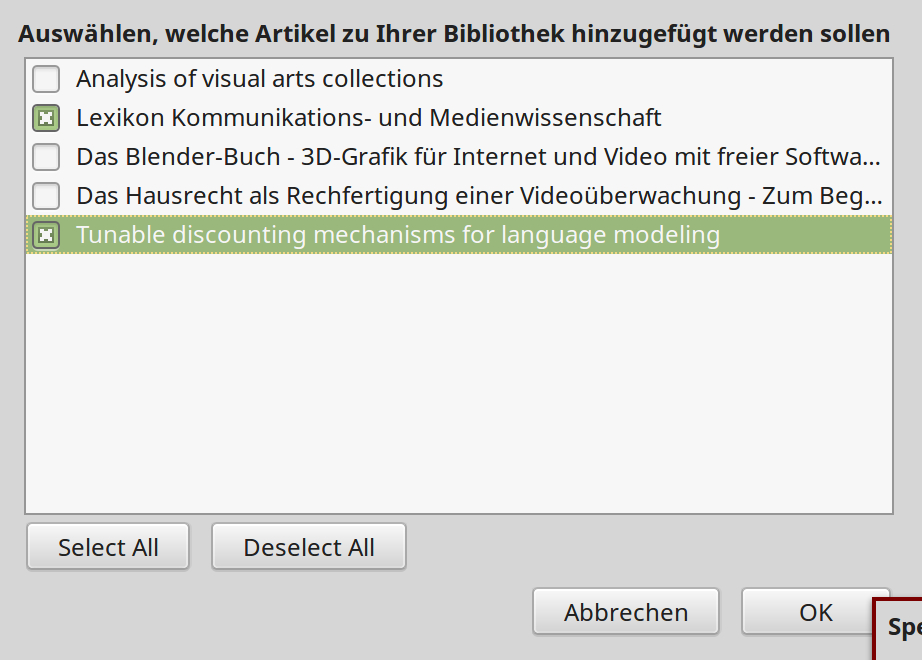
\includegraphics[width=10cm]{Bilder/Kapitel7/Zotero_Eintraege_auswaehlen}}
 \caption{Einträge auswählen}
 \label{fig:eintraegeAuswaehlen}
\end{figure}

\end{enumerate} 
\subsubsection*{Export nach JabRef\index{Export!JabRef}}\label{sss:exportJabref}
\begin{enumerate}
    \item Legen Sie alle Publikationen, die Sie in JabRef\index{JabRef} exportieren möchten in Ihre Anlage.
    \item Klicken Sie aus das Exportzeichen oben rechts in der Ablage und wählen Sie im Dropdown- Menü das Dateiformat \enquote{BibTex} aus.
    \item Ihre Publikationen werden Ihnen anschließend dem ausgewählten Dateiformat angezeigt. Drücken Sie auf die rechte Maustaste und speichern Sie die Publikationen, indem Sie \enquote{Speichern unter...} wählen, an dem gewünschten Platz. 
    \item Öffnen Sie JabRef und klicken auf den Reiter \enquote{Datei}. 
    \item Es öffnet sich ein Dropdown-Menü. Wählen Sie zwischen den Optionen: \enquote{Importieren in neue Datenbank} oder \enquote{Importieren in aktuelle Datenbank}.
    \item Auf dem Bildschirm erscheint ein Popup-Fenster, indem Sie, die in Schritt 3 abgespeicherte Datei, auswählen können. Bestätigen Sie anschließend Ihre Wahl mit \enquote{Öffnen}. Die Publikationen werden Ihnen in der ausgewählten Datenbank automatisch angezeigt.
\end{enumerate}

\section{Literaturlisten importieren}
\label{sec:llImportieren}
Das Importieren\index{Import} von Literaturlisten aus anderen Programmen in PUMA ist jederzeit möglich. Das gängigste Datenformat, das die meisten Programme unterstützen, ist BibTex\index{BibTex}. \newline 
Der Import erfolgt in zwei Schritten. Exportieren Sie zuerst die gewünschten Publikationen aus dem Litertaurverwaltungsprgramm, bevor Sie sie anschließend nach PUMA importieren. 
\subsection{BibTex-Export aus verwendeten Literaturverwaltungsprogrammen}
\label{subsec:bibtexExport}
\subsubsection*{Bib-TeX-Export aus Citavi\index{Import!Citavi}}\label{sss:importCitavi} 
\begin{enumerate}
    \item Klicken Sie bei Citavi\index{Citavi} oben rechts auf \enquote{Datei}, dann im Dropdown-Menü auf \enquote{Exportieren}.
    \item Ein Dialog erscheint. Wählen Sie aus, ob Sie nur den markierten oder alle Artikel exportieren möchten. Klicken Sie dann im Dialog unten auf \enquote{Weiter}.

\begin{figure}[h!]
 \centering
 \fbox{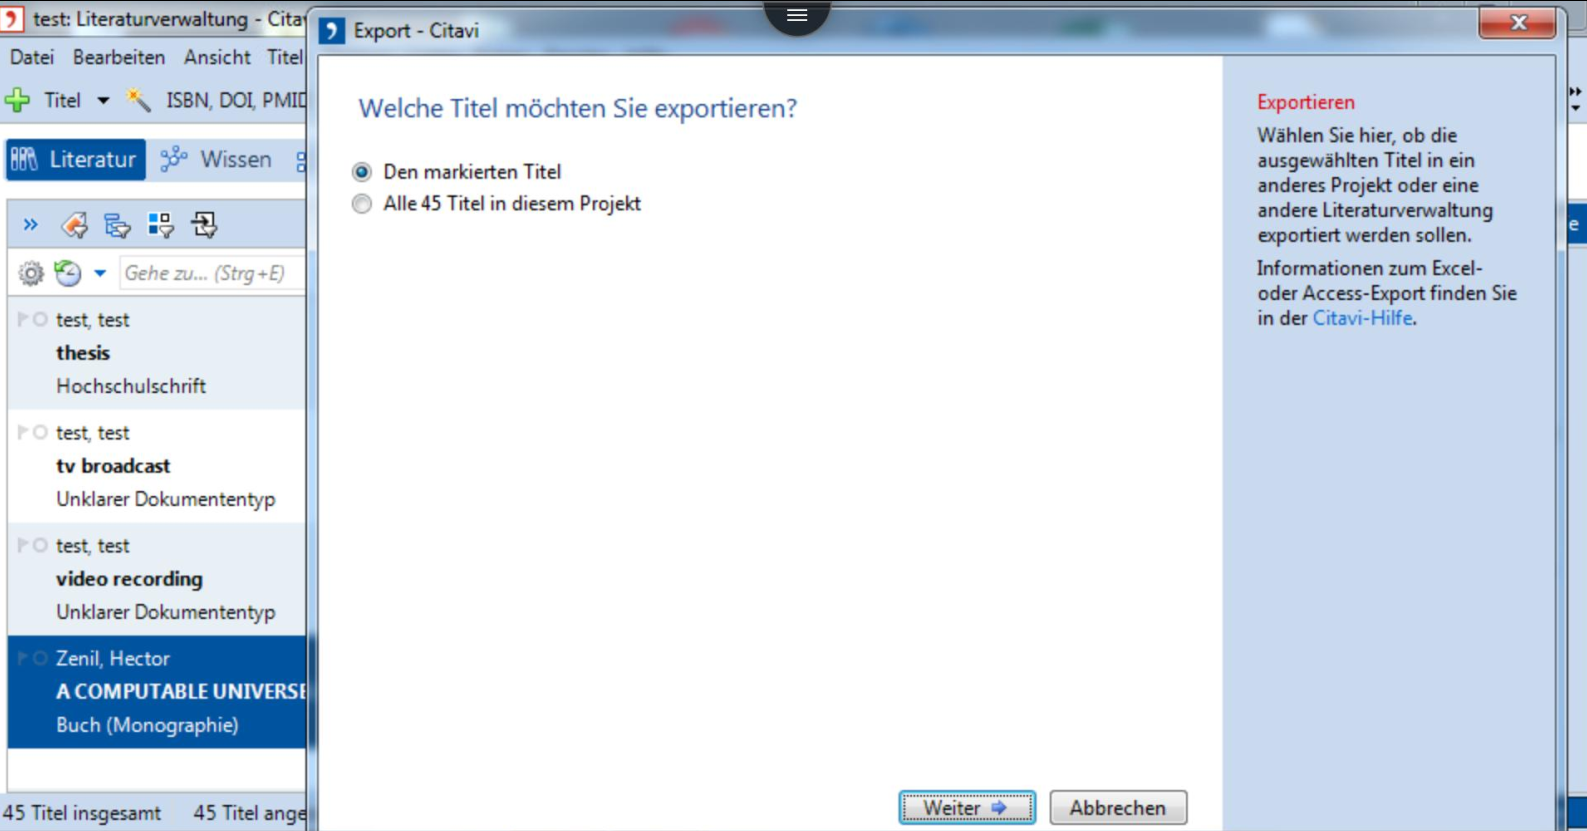
\includegraphics[width=9cm]{Bilder/Kapitel7/Citavi_Schritt2}}
 \caption{Auswählen der zu exportierenden Artikel}
 \label{fig:exportierendenArtikelAuswaehlen}
\end{figure}
    \item Im nächsten Schritt werden Sie nach dem Export-Format gefragt, wählen Sie hier \enquote{BibTex} aus und klicken anschließend auf \enquote{Weiter}.
  
\begin{figure}[h!]
 \centering
 \fbox{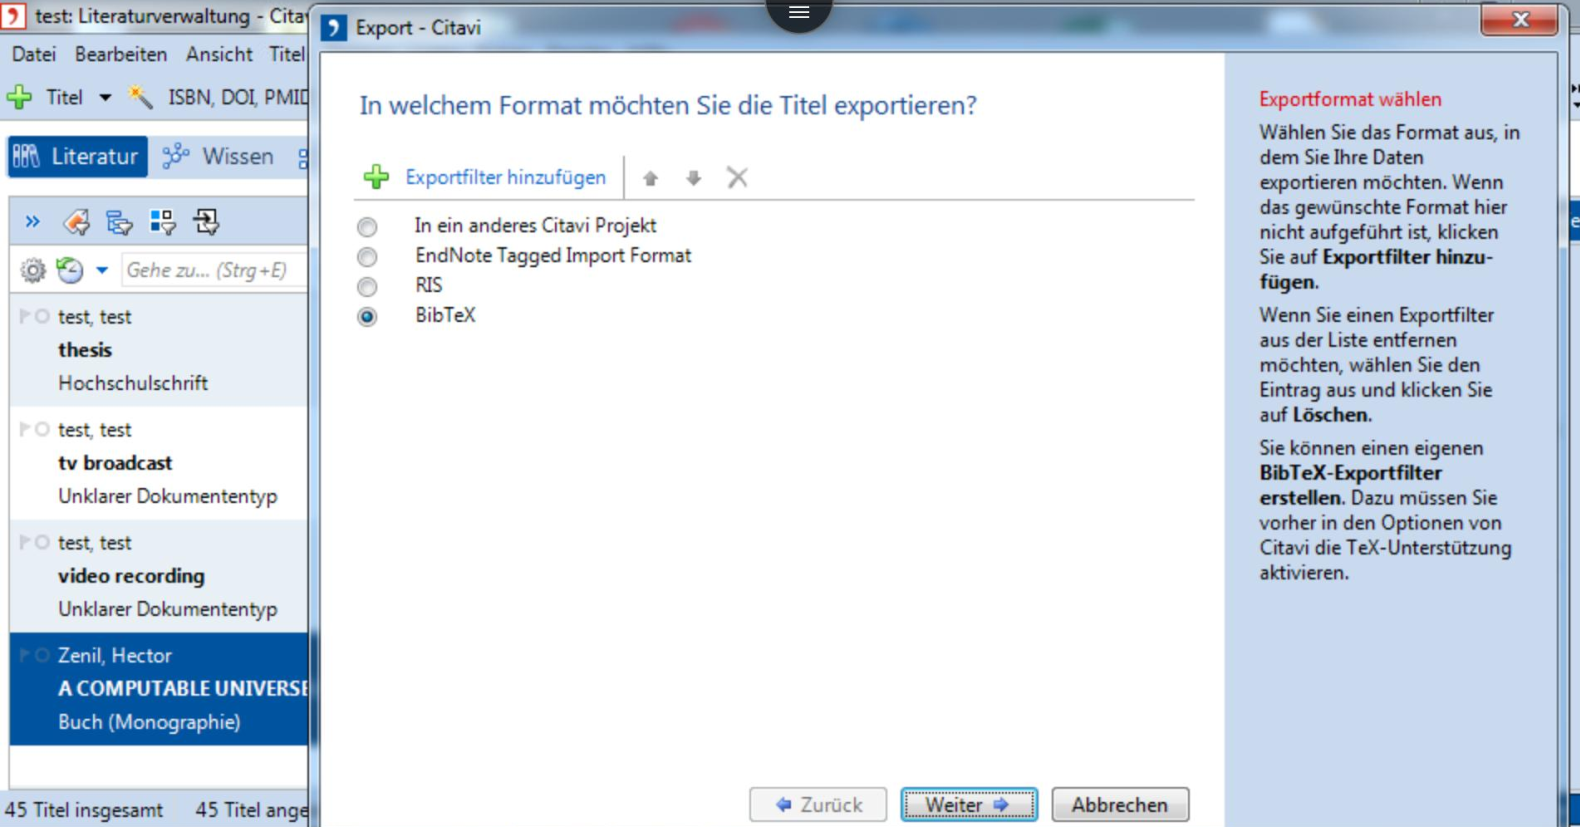
\includegraphics[width=9cm]{Bilder/Kapitel7/Citavi_Schritt3}}
 \caption{Export-Format festlegen}
 \label{fig:exportFormatFestlegen}
\end{figure}
    \item Sie werden nach dem Speicherort gefragt, wählen Sie hier \enquote{Textdaten in der Zwischenablage speichern}. Klicken Sie anschließend auf \enquote{Weiter}.
   
\begin{figure}[h!]
 \centering
 \fbox{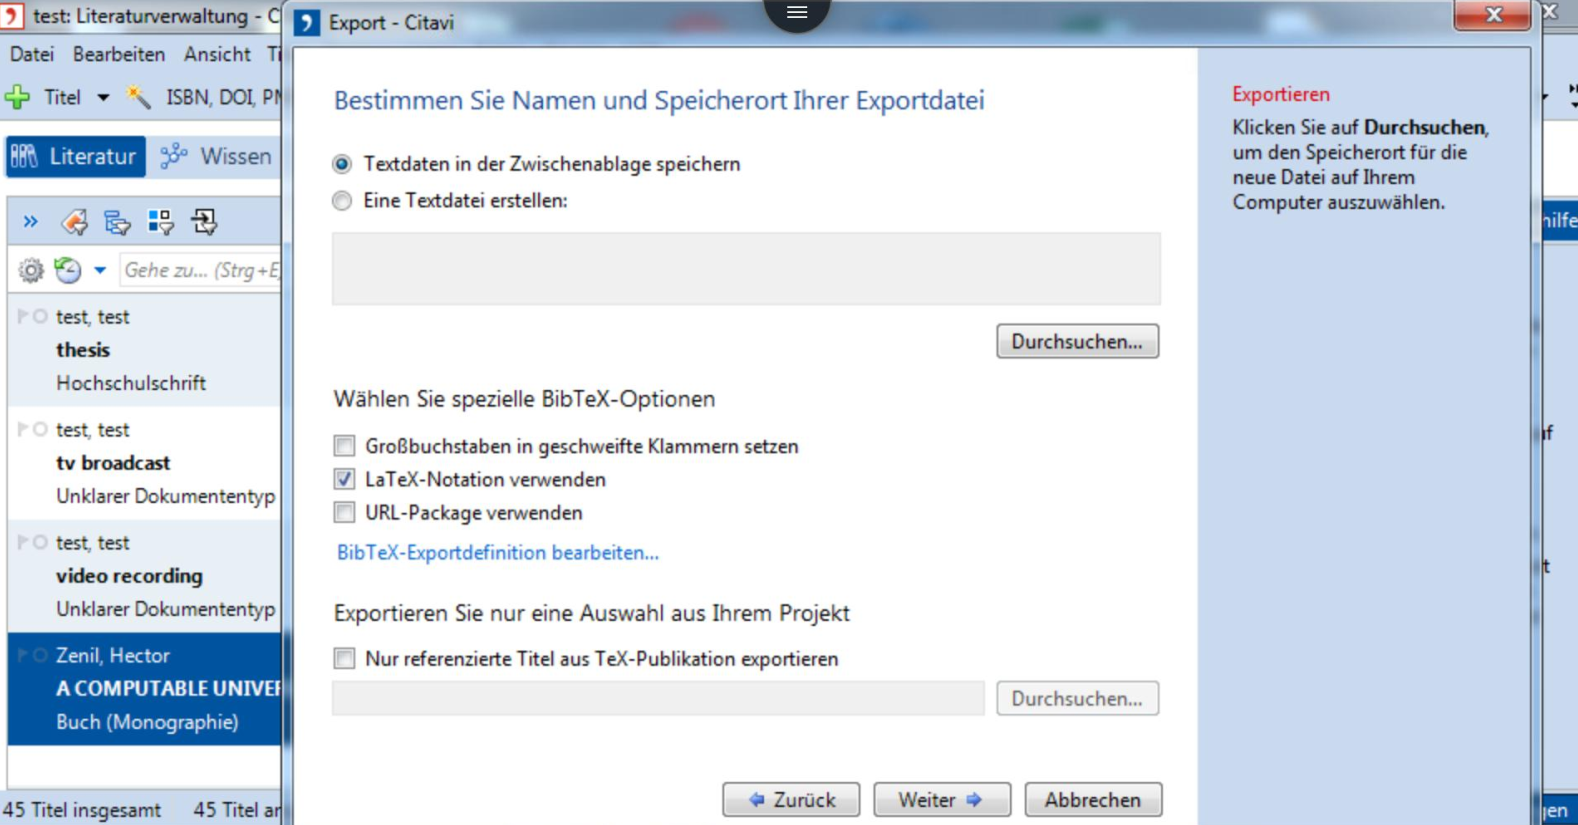
\includegraphics[width=9cm]{Bilder/Kapitel7/Citavi_Schritt4}}
 \caption{Speicherort}
 \label{fig:speicherort}
\end{figure}
    \item Anschließend werden Sie gefragt, ob Sie die Export-Vorlage speichern möchten. Wählen Sie hierfür \enquote{Ja, unter dem Namen:} aus und tragen in das Textfeld \textit{BibTex} als Namen ein. Klicken Sie anschließend auf \enquote{Weiter}.
   
\begin{figure}[h!]
 \centering
 \fbox{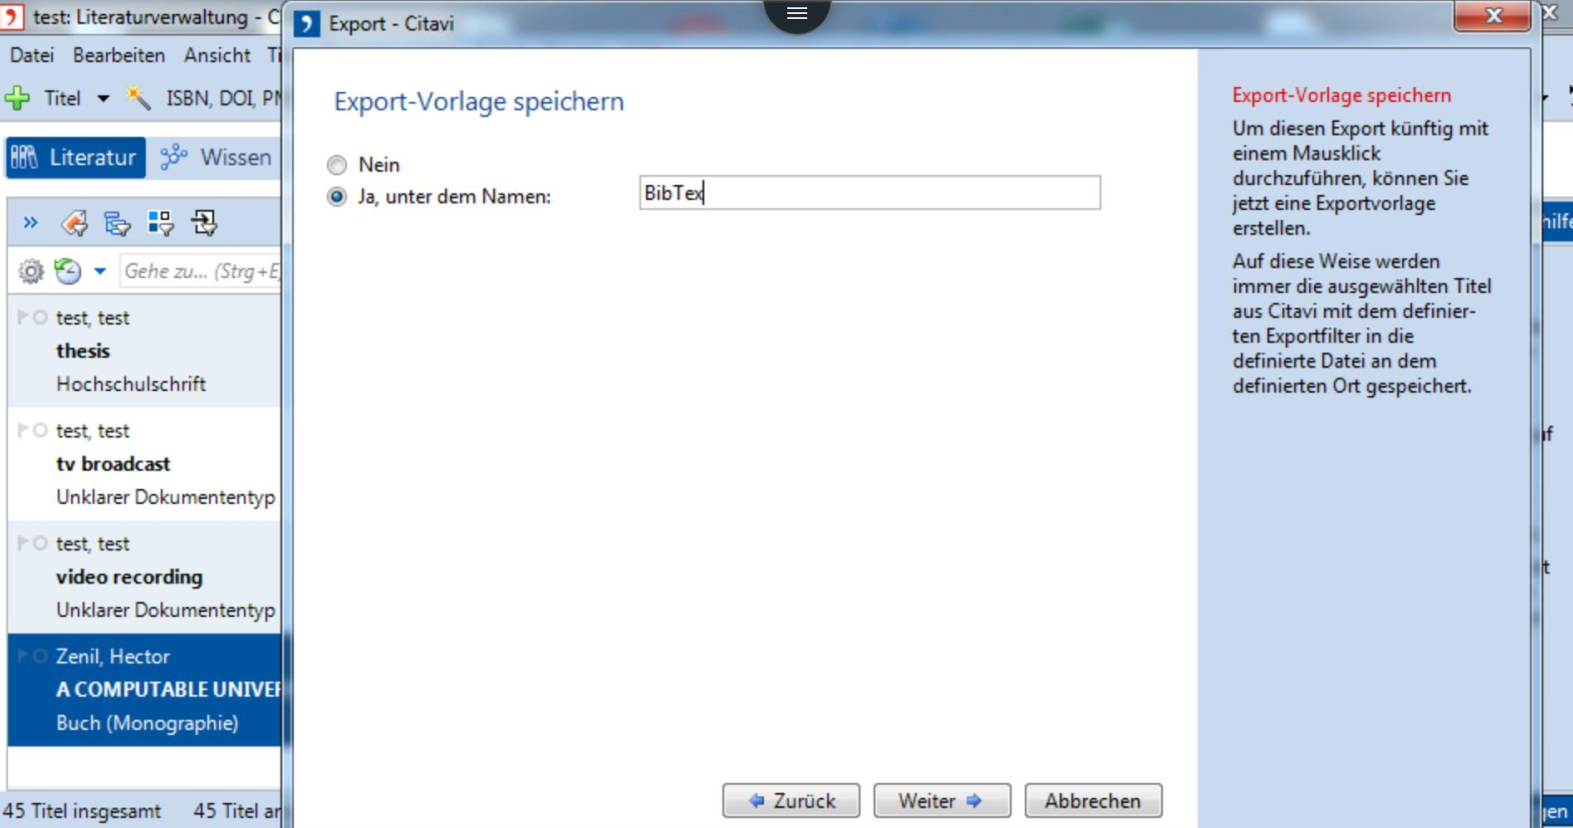
\includegraphics[width=9cm]{Bilder/Kapitel7/Citavi_Schritt5}}
 \caption{Export-Vorlage speichern}
 \label{fig:exportVorlageSpeichern}
\end{figure}
    \item Es öffnet sich ein Popup-Fenster \enquote{Export erfolgreich abgeschlossen}. Bestätigen Sie den Export mit \enquote{OK}.
\end{enumerate}
Die von Ihnen exportierten Daten befinden sich nun in der Zwischenablage. Fahren Sie mit Schritt 1 von BibTex aus der Zwischenablage importieren fort, um Ihre Daten endgültig nach PUMA zu exportieren.\newline

\subsubsection*{Import aus Zotero\index{Import!Zotero}} \label{sss:importZotero}

Um den Import von Zotero\index{Zotero} zu PUMA möglich zu machen, muss Zotero erst einmal für PUMA konfiguriert werden. In den folgenden Schritten erfahren Sie, wie Sie genau vorgehen müssen:
\begin{enumerate}
    \item Öffnen Sie Zotero, indem Sie oben rechts bei Firefox auf das Zotero-Symbol klicken.
    \item Ändern Sie die Einstellungen, indem Sie auf das schwarze Zahnrad klicken. 
\begin{figure}[h!]
 \centering
 \fbox{\includegraphics[width=9cm]{Bilder/Kapitel7/Zotero_Import}}
 \caption{Import aus Zotero}
 \label{fig:importZotero}
\end{figure}
    \item Wählen Sie im Dropdown-Menü \enquote{Einstellungen} aus.
    \item Es öffnet sich ein Popup-Fenster, wählen Sie hier den Menüpunkt \enquote{Export} aus.
\begin{figure}[h!]
 \centering
 \fbox{\includegraphics[width=9cm]{Bilder/Kapitel7/Zotero_Menuepunkt_Export}}
 \caption{Menüpunkt Export}
 \label{fig:menueExport}
\end{figure} 
    \item Fügen Sie zu den Website-Spezifischen Einstellungen, durch klicken auf das \enquote{ '+'-Symbol}, einen neuen Eintrag hinzu. Geben Sie in dem Popup-Fenster \textit{puma.ub.uni-stuttgart.de} ein und wählen Sie \textit{BibTeX\index{BibTex}} als Ausgabeformat. Bestätigen Sie den Eintrag mit \enquote{OK}. 
\end{enumerate}
Nachdem Sie die Konfiguration vorgenommen haben, können Sie die Publikationen nach PUMA importieren. 
\begin{enumerate}
    \item Klicken Sie im Hauptmenü auf \enquote{Eintragen} und wählen im Dropdown-Menü die Option \enquote{Publikation eintragen} aus.  
    \item Klicken Sie auf den Reiter \enquote{BibTex\index{BibTex}/EndNote\index{EndNote}-Schnipsel}. In das Feld \enquote{Auswahl} können Sie nun den entsprechenden Eintrag aus Ihrer Zotero-Bibliothek durch Drag und Drop hineinziehen (klicken Sie auf den Zotero-Eintrag, halten Sie die linke Maustaste gedrückt, bewegen Sie den Mauszeiger in das Feld und lassen Sie dann die linke Maustaste los). Durch Klicken auf \enquote{Weiter} werden die Daten aus dem Zotero-Eintrag extrahiert und in die entsprechenden Felder eingetragen. 
\begin{figure}[h!]
 \centering
 \fbox{\includegraphics[width=10cm]{Bilder/Kapitel7/Zu_PUMA_importieren}}
 \caption{Zu PUMA importieren}
 \label{fig:zuPumaImportieren}
\end{figure}
    \item Klicken Sie anschließend auf \enquote{Speichern} um den Eintrag in Ihre Sammlung zu übernehmen.
\end{enumerate}  
\subsubsection{Import aus JabRef\index{Import!JabRef}\index{JabRef}}\label{sss:importJabRef}
\begin{enumerate}
    \item Klicken Sie mit der rechten Maustaste auf die Publikation, die Sie nach PUMA importieren möchten.
    \item Es erscheint ein Dialog. Wählen Sie \enquote{In die Zwischenablage kopieren} aus.
    \item Im nächsten Schritt werden Sie nach dem Export-Format gefragt, wählen Sie hier \enquote{Endnote} aus.
\end{enumerate}
Die von Ihnen exportierte Publikation befindet sich nun in der Zwischenablage. Fahren Sie mit Schritt 1 von BibTex/~EndNote aus der Zwischenablage importieren fort, um Ihre Publikation endgültig nach PUMA zu exportieren.

\subsection{BibTex\index{BibTex}/ EndNote\index{EndNote} aus der Zwischenablage importieren}
\label{subsec:bibtexImportieren}
Voraussetzung ist, dass Sie Ihre Literaturliste aus Ihrem bisherigen Literaturverwaltungsprogramm in die Zwischenablage exportieren.
\begin{enumerate}
    \item Klicken Sie auf den Menüpunkt \enquote{Eintragen} im Hauptmenü. Ein Untermenü klappt auf.
    \item Klicken Sie im Untermenü auf \enquote{Publikation eintragen}.
    \item Klicken Sie auf den Reiter \enquote{BibTex/~EndNote-Schnipsel}.
    \item Fügen Sie den Text aus der Zwischenablage in das Textfeld \enquote{Auswahl} ein. Dies können Sie so erreichen, indem Sie auf das Textfeld Auswahl gehen und mit der rechte Maustaste das Menü öffnen und auf \enquote{Einfügen} klicken. Erscheint das \enquote{Einfügen} grau, dann haben Sie keine Daten in die Zwischenablage exportiert und Sie müssen den Text erneut in die Zwischenablage einfügen.
    \item Klicken Sie auf \enquote{Weiter}.
    \item PUMA zeigt Ihnen nun eine Übersicht über alle Daten an. Überprüfen Sie diese auf ihre Richtigkeit.
    \item Klicken Sie \enquote{Speichern}.
\end{enumerate}
\section{RSS-Feed abonnieren} 
\label{sec:rssFeedAbonnieren}
RSS\index{RSS} (engl. Really Simple Syndication)-Feeds sind Dateienformate, die Ihnen Veränderungen auf Websites zeigen. So werden Sie immer über Neuigkeiten informiert. Für PUMA bedeutet der RSS-Feed, dass Sie eigene oder fremde Publikations-/~Lesezeichenlisten abonnieren können. Dies funktioniert auch mit Publikationslisten von Gruppen. Nach dem Abonnieren werden Sie über jede Neuigkeit (z.~B. Neue Einträge) informiert. 
\begin{enumerate}
    \item Klicken Sie auf das Exportzeichen in der Publikations-/~Lesezeichenspalte, die Sie abonnieren wollen. Es öffnet sich ein Dropdown- Menü.
\begin{figure}[h!]
 \centering
 \fbox{\includegraphics[width=10cm]{Bilder/Kapitel7/RSS-feed_abonnieren}}
 \caption{RSS-Feed abonnieren}
 \label{fig:rssFeedAbbonnieren}
\end{figure}
    \item  Klicken Sie auf \enquote{RSS}. Der RSS-Feed wird erzeugt und an Ihren RSS-Reader weitergeleitet. 
\begin{mdframed}[style=mdfexample1,frametitle={\texttt{ACHTUNG}},backgroundcolor=gray!40]\texttt{Das weitere Vorgehen ist exemplarisch, es richtet sich sowohl nach Ihrem Webbrowser als auch nach Ihrem RSS-Reader. Im gezeigten Fall übernimmt der Browser \enquote{Mozilla Firefox} sowohl die Aufgabe des Webbrowsers als auch die des RSS-Readers.}
\end{mdframed}
    \item Es werden Ihnen von Mozilla Firefox einige Optionen zum Abonnieren angeboten. Wählen Sie hier \enquote{Dynamische Lesezeichen} und klicken Sie anschließend auf \enquote{Jetzt abonnieren}.
\begin{figure}[h!]
 \centering
 \fbox{\includegraphics[width=11cm]{Bilder/Kapitel7/RSS_dynamisches_Lesezeichen}}
 \caption{Das dynamische Lesezeichen}
 \label{fig:dynamischesLesezeichen}
\end{figure}
    \item Ein Pop-Up Fenster öffnet sich. Wählen Sie einen Namen für den RSS-Feed aus. PUMA generiert immer automatisch einen Namen, diesen können Sie übernehmen.
    \item Wählen Sie den Ordner aus, in dem der RSS-Feed gespeichert werden soll.
    \item Klicken Sie abschließend auf \enquote{Abonnieren}, um den Feed zu abonnieren/speichern.
\end{enumerate}
Dies ist nun die Ansicht des RSS-Feeds-Readers im Vergleich zur Ansicht in PUMA:
\begin{figure}[h!]
 \centering
 \fbox{\includegraphics[width=11cm]{Bilder/Kapitel7/RSS-Reader}}
 \caption{Der RSS-Reader}
 \label{fig:rssReader}
\end{figure}
\section{Universitätsbibliografie\index{Unibibliografie}}
\label{sec:unibibliografie}
Die Universitätsbibliografie (kurz: Unibibliografie) bietet eine möglichst vollständige Übersicht über die Publikationen, die an der Universität Stuttgart veröffentlicht werden. Seit 2015 werden sämtliche Publikationen aller wissenschaftlichen Mitglieder (nach §9 LHG) der Universität Stuttgart hier gezeigt, die während und ggf. nach ihrer Zugehörigkeit zur Universität verfasst bzw. herausgegeben, öffentlich und dauerhaft verfügbar gemacht wurden.\newline\newline
Geführt wird die Unibibliografie der Universität Stuttgart über PUMA. Für die Mitglieder der Universität besteht zukünftig auch die Möglichkeit ihre Publikationen über PUMA zu melden. Die Universitätsbibliothek bearbeitet die Datensätze und veröffentlicht diese Publikationsmetadaten in der Gruppe \textit{unibibliografie} in PUMA. Das System bietet sehr viele Möglichkeiten, die gewünschten Daten zu exportieren. Weitere Informationen finden Sie auf der Homepage der Universitätsbibliothek Stuttgart. \footnote{\url{http://www.ub.uni-stuttgart.de/forschen-publizieren/unibibliografie/}}
\section{OPUS}
\label{sec:opus}
\subsection{Über OPUS}
\label{subsec:ueberOpus}
OPUS ist der Dokumentenserver (das institutionelle Repositorium) der Universität Stuttgart. Die Möglichkeit, über OPUS zu veröffentlichen ist, ist derzeit noch in der Planung. Alle Angehörigen der Universität Stuttgart können in der Zukunft über OPUS ihre Dokumente, die von dauerhaftem Interesse für Forschung und Lehre sind, online im Sinne von Open Access\index{Open Access} veröffentlichen.
\newline\newline
Es wird die Möglichkeit bestehen, dass die Nutzer von PUMA aus in OPUS\index{OPUS} veröffentlichen können. Bei der Aktivierung des Tags \textit{myown}, wird den Nutzern automatisch die Veröffentlichung auf OPUS angeboten werden. Durch diesen Schritt werden ihre Publikationen im Internet langfristig und weltweit frei zugänglich. Dadurch werden die Veröffentlichungen auch in Bibliothekskatalogen, Datenbanken und allen gängigen Suchmaschinen nachgewiesen und somit die Sichtbarkeit der Publikationen deutlich erhöht.
\newline\newline
Die Zitierfähigkeit der Veröffentlichungen wird durch eine dauerhafte, stabile Internet-Adresse (Persistent Identifier) garantiert.
\newline\newline
Mit dem Repositorium wird der von der Universität Stuttgart geförderte freie Zugang zu wissenschaftlicher Information (Open Access) unterstützt werden.
%\subsection{OPUS und PUMA}
%\label{subsec:opusPuma}
%Beim Eintragen einer Veröffentlichung/Publikation in PUMA wird die eigene Veröffentlichung mit \textit{myown} getaggt. Sie werden von PUMA gefragt, ob Sie auf OPUS veröffentlichen wollen. Wenn Sie diese Frage mit \enquote{Ja} bestätigen, wird eine SWORD-Datenverbindung\index{SWORD} zur Sherpa/Romeo-Liste\index{Sherpa/Romeo-Liste} hergestellt. Diese zeigt an, was die Verlage im Bezug auf die Veröffentlichung erlauben. Ist das Hochladen \enquote{grün}, so wird die Veröffentlichung auf OPUS  hochgeladen (so genanntes \enquote{Self Archiving}).
%\newline \newline
%Die Sherpa/Romeo-Liste\footnote{\url{http://www.sherpa.ac.uk/romeo/index.php}} ist eine Datenbank in Manchester, über die die Verlagskonditionen für Zweitveröffentlichungen abgefragt werden können. Bei deutschen Verlagen gilt ein Zeitfenster von 12 Monate nach Erstveröffentlichung, bevor die Autoren eine Zweitveröffentlichung machen können (Grüner Weg des Open Access). Bei Verlagen im Ausland gelten z. T. deutlich höhere Schutzfristen.
\section{DBLP}
\label{dblp}
Das Digital Bibliography \& Library Project (DBLP\index{DBLP}; zu deutsch: Digitales Bibliographie- und Bibliotheksprojekt) ist eine online verfügbare bibliographische Datenbank. In der Sammlung befinden sich mehr als 3 Mio. unterschiedliche wissenschaftliche Publikationen aus dem Bereich Informatik.\newline
PUMA und BibSonomy sind mit der DBLP-Datenbank verbunden. Die Datenbank wird mehrmals wöchentlich aktualisiert und stellt PUMA und BibSonomy Publikationen zur Nachnutzung zur Verfügung. \newline
Die Nutzer können so, die in PUMA hochgeladenen Publikationen und Lesezeichen nachnutzen und mit ein paar Klicks in die eigenen Sammlung übernehmen. 

\chapter{Zusammenarbeit und soziale Funktion}
\label{ch:zusammenarbeit}
\textit{Bei PUMA kommt die soziale Komponente natürlich nicht zu kurz. Ob in gemeinsamen Gruppen oder als Freunde, in PUMA lässt es sich gemeinsam arbeiten.}
\section{Freunde}% Screenshot von beiden Seiten (Menü und nutzerseite)
\label{sec:freunde}
PUMA bietet den Nutzern die Möglichkeit, andere Nutzer als Freunde zu kennzeichnen.  Freundschaften\index{Freunde} ermöglichen das Teilen von Publikationen und Lesezeichen. Wählen Sie in der Sichtbarkeitseinstellung eines Eintrags \enquote{andere} und dann \enquote{friends} aus, können Ihre Freunde diesen Eintrag sehen. Auf die gleiche Weise können Ihre Freunde Einträge für Sie sichtbar machen. Einen Überblick über diese Einträge erhalten Sie über den Menüeintrag \enquote{meinPUMA} (\autoref{subsec:meinPuma}) unter \enquote{Einträge von Freunden}.\newline

\subsection{Freund hinzufügen}
\label{subsec:freundHinzu}

\begin{enumerate} 
    \item Gehen Sie auf die Seite der Person, die Sie als Freund hinzufügen möchten, indem Sie ihren Benutzernamen anklicken oder nach ihr suchen.
		
		\begin{description}
		\item [Benutzername anklicken] Sie finden den Nutzernamen bei jedem Eintrag, den diese Person angelegt hat, beginnend mit einem @ (siehe \autoref{fig:benutzerAnklicken}). Klicken Sie auf den Benutzernamen, um auf seine Seite zu gelangen.
		
		\begin{figure}[h!]
 \centering
 \fbox{\includegraphics[width=5cm]{Bilder/Kapitel8/Benutzername_in_Eintrag.png}}
 \caption{Benutzername anklicken}
 \label{fig:benutzerAnklicken}
\end{figure}
		\item [Nutzer suchen] Wählen Sie im Drop-Down-Menü der Suchleiste (\autoref{sec:suche}) \enquote{Benutzer} aus und geben Sie den Benutzernamen der gewünschten Person ins Textfeld ein.
		\begin{figure}[h!]
 \centering
 \fbox{\includegraphics[width=11cm]{Bilder/Kapitel8/Benutzer_suchen}}
 \caption{Benutzer suchen}
 \label{fig:benutzerSuchen}
\end{figure}

	\end{description}
    \item Sie gelangen auf die Seite des Nutzers, auf der alle seine öffentlichen Einträge zu sehen sind. In der rechten Spalte der Seite wird Ihnen der Benutzer angezeigt. Klicken Sie auf \enquote{Freund hinzufügen}.
\end{enumerate}

\begin{figure}[h!]
 \centering
 \fbox{\includegraphics[width=11cm]{Bilder/Kapitel8/Nutzerseite}}
 \caption{Die Nutzerseite}
 \label{fig:nutzerseite}
\end{figure}

\subsection{Freundesübersicht}
\label{subsec:freundesuebersicht}
Die Freundesübersicht bietet Ihnen einen Überblick über Ihre Freunde in PUMA. Sie gelangen zu der Übersicht über das Dropdown-Menü des Personensymbols. Klicken Sie auf den Reiter \enquote{Freunde}. Sie erhalten nun einen Überblick über Ihre Freunde und können auch sehen, welche Nutzer Sie als Freund angegeben haben. Am Ende der Seite sind alle Publikationen aufgelistet, die Ihre Freunde mit Ihnen oder Sie mit Ihren Freunden teilen.\newline
\begin{figure}[h!]
 \centering
 \fbox{\includegraphics[width=11cm]{Bilder/Kapitel8/Freundesuebersicht}}
 \caption{Freundesübersicht}
 \label{fig:freundesuebersicht}
\end{figure}
Es besteht jederzeit die Möglichkeit, Freunde wieder zu entfernen. Gehen Sie hierfür mit der Maus auf den jeweiligen grünen Kasten \enquote{Freund} des Freundes, den Sie entfernen möchten. Der Kasten wird sich von Grün zu Rot verändern und Sie können durch einen Klick auf die linke Maustaste den Freund entfernen. 
\section{Gruppen}
\label{sec:gruppen}
Gruppen\index{Gruppen} vereinfachen die Zusammenarbeit auf Puma. Sie ermöglichn eine gemeinsame Literaturrecherche und erleichtern so die Umsetzung von gemeinsamen Projekten. Gleichzeitig kann innerhalb einer Institution oder Arbeitsgruppe der Austausch über neue, interessante, fremde oder eigene Artikel mit Hilfe von PUMA erfolgen und somit die Kommunikation vereinfacht werden. 
\subsection{Gruppen \index{Gruppen!beitreten}suchen und beitreten}
\label{subsec:gruppenSuchenBeitreten}
\begin{figure}[h!]
 \centering
 \fbox{\includegraphics[width=11cm]{Bilder/Kapitel8/Gruppen-Uebersichtsseite}}
 \caption{Allgemeine Liste}
 \label{fig:allgemeineListe}
\end{figure}
\begin{enumerate}
    \item Klicken Sie auf \enquote{Gruppen} im Hauptmenü. Ein Dropdown-Menü öffnet sich.
    \item Klicken Sie im Dropdown-Menü auf \enquote{Alle Gruppen}.
    \item Es öffnet sich eine Übersicht über alle Gruppen bei PUMA in alphabetischer Reihenfolge. Rechts neben dem jeweiligen Gruppennamen befindet sich ein Button, um der Gruppe beizutreten. Klicken Sie auf den Beitreten-Button der gewünschten Gruppe.
\begin{figure}[h!]
 \centering
 \fbox{\includegraphics[width=11cm]{Bilder/Kapitel8/Beitreten_einer_Gruppe}}
 \caption{Beitreten einer Gruppe}
 \label{fig:gruppeBeitreten}
\end{figure}
    \item Eine neue Seite erscheint. Geben Sie in das Feld \enquote{Begründung} ein, warum Sie der Gruppe beitreten möchten.
    \item Geben Sie den angezeigten Captcha-Text in das vorgegebene Feld ein. Damit soll verhindert werden, dass Programme automatisiert Gruppen beitreten. 
    \item Klicken Sie anschließend auf \enquote{Anfrage absenden}.
    \item Der Gruppen-Administrator erhält eine E-Mail-Benachrichtigung, dass Sie in die Gruppe eintreten wollen. Allein der Administrator entscheidet über die Aufnahme, weswegen ein plausibler Begründungstext sinnvoll ist.
\end{enumerate}
In der E-Mail, die alle Administratoren erhalten, befindet sich ein Link (erster Link in der E-Mail). Durch das Anklicken des Links öffnet sich die Einstellungsseite der Gruppe. Der Administrator kann nun den Nutzer aufnehmen oder dessen Beitrittsanfrage ablehnen.
\subsection{Gruppen erstellen\index{Gruppen!erstellen}}
\label{subsec:gruppenErstellen}
\begin{enumerate}
    \item Klicken Sie im Hauptmenü auf \enquote{Gruppen}. Ein Dropdown-Menü öffnet sich.
    \item Klicken Sie im Dropdown-Menü auf \enquote{Eine neue Gruppe erstellen}.
\begin{figure}[h!]
 \centering
 \fbox{\includegraphics[width=11cm]{Bilder/Kapitel8/Neue_Gruppe_erstellen}}
 \caption{Erstellung einer neuen Gruppe}
 \label{fig:erstellungNeueGruppe}
\end{figure}
    \item Geben Sie einen Gruppennamen und eine Beschreibung der Gruppe an. 
    \item Klicken Sie anschließend auf \enquote{Gruppe erstellen}. 
\end{enumerate}
Ab sofort können Sie die Vorteile der gemeinsamen Literaturrecherche von PUMA nutzen und Publikationen für spezielle Gruppen sichtbar machen. Dies legen Sie beim Eintragen einer neuen Publikation oder eines neuen Lesezeichens fest, indem Sie bei der Sichtbarkeit\index{Sichtbarkeit} unter dem Punkt \textit{andere} die spezielle Gruppe auswählen. Wenn Sie diese Publikation nun speichern, sehen diese automatisch alle Gruppenmitglieder.
\subsection{Die Gruppenseite}
\label{subsec:gruppenseite}
Um zur Gruppenseite\index{Gruppen} zu gelangen, klicken Sie im Dropdown-Menü vom Reiter  \enquote{Gruppen} auf den entsprechenden Namen der Gruppe. Sie gelangen zur Gruppenseite, auf der Sie einen Überblick über alle Lesezeichen und Publikationen erhalten.%Screenshot
\newline\newline
Funktionen auf der Gruppenseite:
\begin{figure}[h!]
 \centering
 \fbox{\includegraphics[width=11cm]{Bilder/Kapitel8/Gruppenseite}}
 \caption{Die Gruppenseite}
 \label{fig:gruppenseite}
\end{figure}
\begin{description}
\item [CV/Lebenslauf der Gruppe] \hfill \\
Durch Klicken auf den CV-Button auf der rechten Seite erhalten Sie alle wichtigen Informationen zu der Gruppe.
\item [Mitglieder-Liste] \hfill \\
Unterhalb des Gruppenbildes befindet sich die Liste aller Mitglieder. 
\item [Diskussionen] Um sich einen Überblick über die diskutierten Einträge zu verschaffen, klicken Sie unter dem Abschnitt Diskussion auf der rechten Seite auf \enquote{Zeige kürzlich diskutierte Einträge von PUMA}. 
\end{description}
 
\subsection{Rollen in einer Gruppe}
\label{subsec:RollenInGruppe}
In einer Gruppe können die unterschiedlichsten Rollen und Aufgaben übernommen werden. In PUMA gibt es drei Rollenarten:
\begin{description}
    \item [Administrator\index{Administrator}:] Er hat die größte Befugnis in der Gruppe. Er ist zuständig für die Einstellungen der Gruppenseite und kann das Layout des Gruppenlebenslaufes editieren. Einträge, die in die Gruppe eingetragen werden, können von Ihm/Ihr bearbeitet werden. Ebenfalls kann er neue Mitglieder einladen und vorhandene ausladen sowie die Rollen der anderen Mitglieder verändern (z.B. weiteren Administrator ernennen).
    \item [Moderator\index{Moderator}:] Der Moderator hat Zugriff auf die Mitgliederliste und kann andere Nutzer in die Gruppe einladen und seine eigene Rolle auf \textit{Nutzer} herabsetzen.
    \item [Nutzer\index{Nutzer}:] Er ist ein Mitglied der Gruppe und hat keine Befugnisse, in der Gruppe Änderungen oder neue Einstellungen vorzunehmen.
\end{description}

\subsection{Einträge für eine Gruppe}
\label{subsec:gruppenfunktion}
Sobald ein Nutzer Mitglied einer Gruppe ist, werden seine öffentlichen Einträge automatisch in der Sammlung der Gruppe angezeigt. Die anderen Mitglieder können diese Publikation aber erst bearbeiten wenn sie die Publikation in Ihre eigene Sammlung übertragen. Eine weitere Möglichkeit, eine Publikation in die Gruppensammlung zu übertragen, bietet das Gruppenoptionsfeld. Damit kann beim Eintragen der Publikation eine Gruppe ausgewählt werden, für die die Publikation interessant ist. Auch diese Einträge können erst dann von den Mitgliedern bearbeitet werden, wenn sie in die eigene Sammlung aufgenommen werden.

Damit andere Mitglieder (Administratoren) einen Eintrag bearbeiten können, muss beim Eintragen der Publikation der Systemtag \textit{for:gruppenname} eingegeben werden. Der Eintrag erscheint wie alle anderen Einträge in der Sammlung der Gruppe. Als Nutzer dieses Eintrags wird der Gruppenname (@gruppenname) angegeben. In der Reihe der Tags erscheint der Systemtag \textit{from:Benutzername}, welcher den genauen Verfasser des Eintrags angibt. In der Detailansicht der Publikation erhalten nun die Administratoren der Gruppe die Möglichkeit, über den schwarzen Stift oben rechts die Publikation zu bearbeiten. Hierfür muss die Publikation nicht in die Sammlung des Administrators übernommen werden.

\section{Community Post}
\label{sec:communityPost}
Ein Community Post\index{Community Post} ist ein Gemeinschaftseintrag, auf den mehrere Personen Zugriff haben. \newline \newline
\textbf{Erstellen eines Community Posts:}
\begin{enumerate}
	\item Klicken Sie auf den Titel der Publikation, um zur Detailansicht der Publikation zu gelangen. 
	\item Gehen Sie mit der Maus auf den kleinen schwarzen Pfeil oben rechts neben dem Publikationstitel. 
	\item Wählen Sie im Dropdown-Menü \enquote{CommunityPost} aus. \end{enumerate}
\begin{figure}[h!]
 \centering
 \fbox{\includegraphics[width=11cm]{Bilder/Kapitel8/Community_post_anlegen}}
 \caption{Community Post anlegen}
 \label{fig:communityPostAnlegen}
\end{figure}
Der Community Post öffnet sich. Sie können nun Änderungen an der Publikation vornehmen, indem Sie oben links auf der Seite auf den Stift klicken, oder weiter unten auf der Community-Seite die Publikation bewerten. Die Änderungen werden in einer Übersicht - der Versionsgeschichte\index{Versionierung} - dargestellt. Zu dieser gelangen Sie oben links, durch einen Klick auf das Verzeichnissymbol.\newline
Durch die Erstellung eines Community Post können Nutzer jederzeit auf die Versionsgeschichte des Eintrages zugreifen und sehen, was und wann von wem geändert wurde. So erleichtert er die Zusammenarbeit und ermöglicht einen umfassenden Überblick. 

Im Bereich \textit{Tags} werden die Tags des Gemeinschaftseintrags angezeigt. Durch einen Klick auf einen Tag werden einem alle Publikationen mit diesem Tag angezeigt.

Unter dem Bereich \textit{Nutzer} werden alle Nutzer angezeigt, die diese Publikation in Ihrer Sammlung eingetragen haben.
\begin{figure}[h!]
 \centering
 \fbox{\includegraphics[width=11cm]{Bilder/Kapitel8/Community_post_Versionsgeschichte}}
 \caption{Versionierung}
 \label{fig:versionierung}
\end{figure}
\section{Nutzern folgen}
\label{sec:nutzernFolgen}
Wie in sozialen Netzwerken bietet PUMA seinen Nutzern die Möglichkeit, anderen Nutzern zu folgen. 

Um einem Nutzer zu folgen, gehen Sie auf dessen Benutzerseite (\autoref{subsec:freundHinzu}). Klicken Sie rechts oben, unterhalb des Benutzerprofilbildes, auf das Feld \enquote{folgen}. Ab sofort sind Sie ein Follower des Nutzers. Sie können jedem Nutzer folgen, egal ob befreundet oder nicht. \newline \newline
Um eine Überblick über die Einträge der verfolgten Person zu erhalten, klicken Sie im Reiter \enquote{meinPUMA} (\autoref{subsec:meinPuma}) auf den Unterpunkt \enquote{verfolgte Einträge}. Es erscheint eine Übersichtsseite mit allen Einträgen der Nutzer, denen Sie folgen. 




%Überarbeiten:neue version anders

\section{Kommentare, Rezensionen und Bewertungen}
\label{sec:kommentare}
PUMA verfügt über die Möglichkeit, Publikationen und Lesezeichen zu bewerten\index{Bewerten} und Rezensionen\index{Rezensionen} zu verfassen. Man kann mit anderen Nutzern über Publikationen/~Lesezeichen diskutieren und seine eigene Meinung zu einer Publikation/~einem Lesezeichen durch die Vergabe von Sternen verdeutlichen.
\newline
\newline
Publikationen/Lesezeichen bewerten:
\begin{enumerate}
    \item Klicken Sie auf die Stern-Leiste (siehe \autoref{fig:sternenleiste}) unterhalb des Lesezeichens oder der Publikation, die Sie bewerten möchten.
\begin{figure}[h!]
 \centering
 \fbox{\includegraphics[width=11cm]{Bilder/Kapitel8/Die_Sternenleiste}}
 \caption{Die Stern-Leiste}
 \label{fig:sternenleiste}
\end{figure}  
    \item Es öffnet sich die Gemeinschaftsseite des Eintrages. Neben den Bereichen \textit{Tags} und \textit{Zitieren Sie diese Publikation} finden Sie hier auch den Bereich \textit{Kommentare und Rezensionen}. \autoref{fig:publikationBewerten} zeigt die Elemente des Bereichs:
\begin{figure}[h!]
 \centering
 \fbox{\includegraphics[width=11cm]{Bilder/Kapitel8/Publikation_bewerten}}
 \caption{Publikation bewerten}
 \label{fig:publikationBewerten}
\end{figure}
    \begin{description} 
        \item [Bewertungsverteilung (A):] Das Balkendiagramm stellt dar, welche Bewertungen wie oft vergeben wurden.  %In diesem Fall ... Beispiel an Hand eines Bildes
        \item [Durchschnittliche Bewertung (B):] In der Stern-Leiste wird der Mittelwert der Bewertungen angezeigt.
        \item [Rezension schreiben (C):] \hfill \\
				Durch einen Klick auf den Button "Rezension schreiben" öffnet sich ein Textfeld, das Ihnen die Möglichkeit bietet, ein Review zu verfassen. Oberhalb des Textfeldes können Sie den Beitrag mit null bis fünf Sternen bewerten. Je höher die Anzahl der Sterne, umso besser ist die Bewertung. Unterhalb des Textfeldes können Sie die Sichtbarkeit Ihrer Bewertung festlegen und so entscheiden, wer sie sehen darf. Es gibt folgende Möglichkeiten:
        \begin{enumerate}
            \item öffentlich: Jeder Nutzer kann Ihre Rezension sehen.
            \item privat: Nur Sie können Ihre Rezension sehen.
            \item Freunde: Sie können einzelne Freunde festlegen, die Ihre Rezension sehen sollen.
            \item Gruppen: Es werden Ihnen alle Gruppen angezeigt, in denen Sie Mitglied sind. Wählen Sie aus, welche Gruppe die Rezension sehen soll.
            \item anonym: Ihr Kommentar wird ohne Ihren Benutzernamen veröffentlicht. Die Bewertung ist für alle Nutzer sichtbar.
        \end{enumerate}
       	Klicken Sie abschließend auf \enquote{Bewerten}, um die Rezension abzuschließen und sie sichtbar zu machen.
        \item [Kommentar schreiben (D):] \hfill \\
				In diesem Textfeld können Sie einen Kommentar verfassen. Ein Kommentar hat die gleichen Möglichkeiten der Sichtbarkeit wie eine Rezension.
\newline Es kann beliebig oft auf Kommentare/~Bewertungen reagiert und geantwortet werden. Neben jedem Kommentar befindet sich ein Button mit einem kleinen schwarzen Pfeil, über den Sie Rezensionen direkt kommentieren können. 
    \end{description}
\end{enumerate}
\chapter{Für Nerds}
\label{ch:fuerNerds}
\textit{Die eigene Sammlung auf der eigenen Homepage veröffentlichen. Mit Hilfe von Pugins, für OpenCms,  und dem JavaScript-Codeschnipsel kein Problem für PUMA.}
\section{URL-Syntax\index{URL-Syntax}}
\label{sec:urlSyntax}
\textbf{Parameter zum Sortieren} \newline
Immer wenn Sie in PUMA Zugriff auf eine Lesezeichen/~Publikationsliste haben, können Sie diese sortieren, indem Sie an die URL einen/~mehrere der folgenden Parameter anhängen. Folgende Parameter stehen Ihnen zur Verfügung:
\begin{enumerate}
    \item \textbf{sortPage - Wonach wird sortiert?}
    \begin{enumerate}
        \item author - Autorenname
        \item editor - Herausgebername
        \item year - Erscheinungsjahr
        \item entrytype - Publikationstyp
        \item title - Titel
        \item booktitle - Buchtitel (insb. bei Artikel in Sammelbänden)
        \item journal - Journalname
        \item school - Universitätsname 
    \end{enumerate}
    \item \textbf{sortPageOrder - Reihenfolge der Sortierung}
    \begin{enumerate}
        \item asc - aufsteigend
        \item desc - absteigend 
    \end{enumerate}
    \item \textbf{duplicates- Duplikate\index{Duplikate}}
    \begin{enumerate}
        \item yes - Erlaubt Duplikate in der Lesezeichen/- Publikationsliste
        \item no - Entfernt Duplikate aus der Ergebnisliste
    \end{enumerate}
\end{enumerate}
%Beispiel: \url{?sortPage=year%\&sortPageOrder=asc\&duplicates=no} \newline
Sortiere nach Erscheinungsjahr (sortPage=~year) aufsteigend (sortPageOrder=~asc) und entferne alle Duplikate (duplicates=~no). \newline
\newline
\textbf{Allgemeine Seiten}
\begin{enumerate}
    \item \textbf{/} \newline
    Homepage von PUMA, zeigt die aktuellsten 50 öffentlichen Einträge.
    \item \textbf{/popular} \newline
    Zeigt die 100 häufigsten Einträge der letzten 100.000 öffentlichen Einträge.
    \item \textbf{/IhrBenutzername} \newline
    Sie gelangen zu Ihrer persönlichen Sammlung.
    \item \textbf{/settings} \newline
    Auf dieser Seite können Sie:
    \begin{enumerate}
        \item Ihr Profil bearbeiten und Kontoeinstellungen ändern,
        \item einen Benutzer zu Ihrer Gruppe hinzufügen,
        \item Ihren API-Schlüssel finden und einen neuen erzeugen,
        \item Ihr Passwort ändern und
        \item Ihre Daten zwischen BibSonomy und PUMA synchronisieren.
    \end{enumerate}
    \item \textbf{/help\_de} \newline
    Sie gelangen zu der Hilfeseite.
    \item \textbf{/postBookmark} \newline
    Hier können Sie über die Eingabe der URL eines Lesezeichen überprüfen, ob sich dieses Lesezeichen schon in Ihrer Sammlung befindet. Durch die Überprüfung können Sie Duplikate vermeiden. Wenn sich das Lesezeichen noch nicht in Ihrer Sammlung befindet, haben Sie im Anschluss an die Überprüfung die Möglichkeit die Metadaten des Lesezeichens einzutragen, um es in Ihre Sammlung auf zu nehmen.
    \item \textbf{/postPublication} \newline
    Auf dieser Seite können Sie neue Publikationen eintragen. 
    \item \textbf{/user/eckert} \newline
    Zeigt alle öffentlichen Einträge des Benutzers \textit{eckert}.
    \item \textbf{/user/eckert/politik} \newline
    Zeigt alle öffentlichen Einträge mit dem Tag \textit{politik} des Benutzers \textit{eckert}.
    \item \textbf{/user/eckert/politik+menschenrechte} \newline
    Zeigt alle öffentlichen Einträge mit dem Tag \textit{politik} und dem Tag \textit{menschenrechte} des Benutzers \textit{eckert}.
     \item \textbf{/myBibTeX} \newline
    Ihnen wird Ihre gesamte Sammlung im BibTex-Format angezeigt.
    \item \textbf{/myRelations} \newline
    Ihnen werden Ihre Konzepte/Relationen angezeigt.
    \item \textbf{/myDuplicates} \newline
    Zeigt Ihre eigenen Duplikaten, die sich in Ihrer Sammlung befinden.
\end{enumerate}    
\subsection{Suchen mit der URL-Syntax}
\label{subsec:suchenMitUrlSyntax}
PUMA bietet Ihnen die Möglichkeit mit Hilfe der URL-Syntax nach bestimmten Seiten zu suchen. Es gibt verschiedene Wege, diese Suchergebnisse zu filtern. Gegenwärtig beinhalten die Filter: Die Tags, den Autor, das Publikationsjahr, den Benutzernamen der Person, die den Eintrag gespeichert hat sowie Freunde- und Gruppennamen. \newline
\newline
\textbf{Tag\index{Tags}-/Schlagwortseiten}
\begin{enumerate}
    \item \textbf{/tag/politik} \newline
    Zeigt alle öffentlichen Einträge mit dem Tag \textit{politik} an.
    \item \textbf{/tag/politik+menschenrechte}\newline
    Zeigt alle öffentlichen Einträge mit dem Tag \textit{politik} und dem Tag \textit{menschenrechte} an.
\end{enumerate}
\textbf{Autorenseiten\index{Autoren}}
\begin{enumerate}
    \item \textbf{/author/müller} \newline
    Zeigt alle Einträge mit dem Autornamen \textit{Müller} an.
    \item \textbf{/author/müller/dblp} \newline
    Zeigt alle Einträge mit dem Tag \textit{dblp} und dem Autor \textit{Müller}.
    \item \textbf{/author/müller/sys:user:eckert}\newline
    Zeigt alle Publikationen des Autors \textit{Müller} in der Sammlung von \textit{Eckert} an.
    \item \textbf{/author/müller/sys:group:puma} \newline
    Zeigt alle Publikationen des Autors \textit{Müller} in der Sammlung aller Gruppenmitglieder der Gruppe \textit{puma} an. 
\end{enumerate}
Ein Systemtag (System-Schlagwort) kann das Ergebnis Ihrer Autoren-Suche auf ein bestimmtes Erscheinungsjahr oder einen bestimmten Zeitraum beschränken. Es sind vier Formate möglich:%muss rausrücken
\begin{enumerate}
    \item \textbf{/author/hotho+sys:year:2007} \newline
    Zeigt alle Publikationen des Autors \textit{Hotho} aus dem Jahre 2007.
    \item \textbf{/author/hotho+sys:year:2003-2007} \newline
    Zeigt alle Publikationen des Autors \textit{Hotho} zwischen 2003 und 2007.
    \item \textbf{/author/hotho+sys:year:-2005} \newline
    Zeigt alle Publikationen des Autors \textit{Hotho} bis zum Jahr 2005 an.
    \item \textbf{/author/hotho+sys:year:1997-} \newline
    Zeigt alle Publikationen des Autors \textit{Hotho} seit 1997 an.
\end{enumerate}
\textbf{Freundeseiten} 
\begin{enumerate}
    \item \textbf{/friends} \newline
    Hier werden die Einträge angezeigt, die nur für Freunde\index{Freunde} sichtbar sind und von Benutzern stammen auf deren Freundesliste Sie stehen.
    \item \textbf{/friend/eckert} \newline
    Hier werden alle Beiträge angezeigt, welche für Freunde des Benutzers \textit{eckert} sichtbar gesetzt sind. Sie können diese Einträge nur dann sehen, wenn \textit{eckert} Sie als Freund angegeben hat.
    \item \textbf{/friend/eckert/politik} \newline
    Zeigt alle Beiträge mit dem Tag \textit{politik} an, welche für Freunde des Benutzers \textit{eckert} sichtbar gesetzt sind. Sie können sie nur dann sehen, wenn \textit{eckert} Sie als Freund angegeben hat.
    \item \textbf{/friend/eckert/politik+menschenrechte} \newline
    Zeigt alle Beiträge mit den Tags \textit{politik} und \textit{menschenrechte} an, welche für Freunde des Benutzers \textit{eckert} sichtbar gesetzt sind. Sie können sie nur dann sehen, wenn \textit{eckert} Sie als Freund angegeben hat.
\end{enumerate}
\textbf{Gruppenseiten\index{Gruppen}}
\begin{enumerate}
    \item \textbf{/groups} \newline
    Zeigt alle Gruppen, die es in PUMA gibt, an.
    \item \textbf{/group/puma} \newline
    Zeigt Ihnen alle Einträge von Mitgliedern der Gruppe \textit{puma} an, wenn Sie Gruppenmitglied sind.
    \item \textbf{/group/puma/politik}\newline
    Zeigt Ihnen alle Einträge mit dem Tag \textit{politik} von Mitgliedern der Gruppe \textit{puma} an, wenn Sie Gruppenmitglied sind.
    \item \textbf{/group/puma/politik+menschnerechte}\newline
    Zeigt Ihnen alle Einträge mit dem Tag \textit{politik} und dem Tag \textit{menschenrechte} von Mitgliedern der Gruppe \textit{puma} an, wenn Sie Gruppenmitglied sind.
    \item \textbf{/relevantfor/group/puma} \newline
    Zeigt Ihnen alle Einträge an,  die für die Teilnehmer der Gruppe relevant sind.
    \item \textbf{/followers} \newline
    Zeigt die neuesten Einträge aller Benutzer, denen Sie folgen. Diese Einträge werden mittels eines Rankings so umsortiert, dass die für Sie relevantesten Einträge ganz oben stehen. 
\end{enumerate}
\textbf{Konzeptseiten}
\begin{enumerate}
    \item \textbf{/concepts/eckert} \newline
    Es werden Ihnen alle Konzepte\index{Konzepte} des Benutzers \textit{eckert} angezeigt.
    \item \textbf{/concept/user/eckert/psychologie} \newline
    Zeigt alle Lesezeichen und Publikationen des Benutzers \textit{eckert} an, denen das Tag \textit{psychologie} oder eines der Unterschlagwörter des Konzeptes als Tag zugeordnet ist. 
\end{enumerate}
\textbf{Suchseiten}\newline
Mit der URL-Syntax \textit{/search...} suchen Sie im Volltext nach einem bestimmten Wort. Es handelt sich dabei nicht um Schlagwörter/Tags. Bei Lesezeichen enthält der Volltext die URL, den Titel und die Beschreibung. Bei Publikationen sind der Titel, die Beschreibung und alle BibTex-Felder enthalten.
\begin{enumerate}
    \item \textbf{/search/politik} \newline
    Zeigt Ihnen alle öffentlichen Einträge an, die im Volltext (nicht in den Schlagwörtern!) das Wort \textit{politik} enthalten. 
    \item \textbf{/search/politik+menschenrechte}\newline
    Zeigt alle öffentlichen Einträge, die im Volltext (nicht in den Schlagwörtern!) das Wort \textit{politik} und das Wort \textit{menschenrechte} enthalten. 
    \item \textbf{/search/politik+-menschenrechte} \newline
    Zeigt alle öffentlichen Einträge an, die im Volltext (nicht in den Schlagwörtern!) das Wort \textit{politik}, aber nicht das Wort \textit{menschenrechte} enthalten. 
    \item \textbf{/search/politik+user:droessler} \newline
    Zeigt alle öffentlichen Einträge des Benutzers \textit{droessler}, die im Volltext (nicht in den Schlagwörtern!) das Wort \textit{politik} enthalten. 
    \item \textbf{/search/politik+menschenrechte+user:droessler}\newline
    Zeigt alle öffentlichen Einträge des Benutzers \textit{droessler} an, die im Volltext (nicht in den Schlagwörtern!) das Wort \textit{politik} und das Wort \textit{menschenrechte} enthalten. 
    \item \textbf{/search/politik+-menschenrechte+user:droessler} \newline
    Zeigt alle öffentlichen Einträge des Benutzers \textit{droessler} an, die im Volltext (nicht in den Schlagwörtern!) das Wort \textit{politik}, aber nicht das Wort \textit{menschnerechte} enthalten. 
    \item \textbf{/mySearch} \newline
    Diese Seite bietet eine Schnellsuche in Ihrer eigenen Sammlung.
\end{enumerate}
\textbf{Sichtbare Seiten\index{Sichtbarkeit}}
\begin{enumerate}
    \item \textbf{/viewable/public} \newline
    Zeigt alle Ihre Einträge an, die Sie als \enquote{öffentlich sichtbar\index{Sichtbarkeit!öffentlich}} eingestellt haben.
    \item \textbf{/viewable/public/politik} \newline
    Zeigt alle Ihre Einträge mit dem Tag \textit{politik} an, die Sie als \enquote{öffentlich sichtbar} eingestellt haben.
    \item \textbf{/viewable/public/politik+menschenrechte} \newline
    Zeigt alle Ihre Einträge mit dem Tag \textit{politik} und dem Tag \textit{menschenrechte}, die Sie als \enquote{öffentlich sichtbar} eingestellt haben.
    \item \textbf{/viewable/private} \newline
    Zeigt alle Ihre Einträge, die Sie als \enquote{privat sichtbar\index{Sichtbarkeit!privat}} eingestellt haben.
    \item \textbf{/viewable/private/politik} \newline
    Zeigt alle Ihre Einträge mit dem Tag \textit{politik} an, die Sie als \enquote{privat sichtbar} eingestellt haben.
    \item \textbf{/viewable/private/politik+menschenrechte} \newline
    Zeigt alle Ihre Einträge mit dem Tag \textit{politik} und dem Tag \textit{menschenrechte} an, die Sie als \enquote{privat sichtbar} eingestellt haben.
    \item \textbf{/viewable/friends} \newline
    Zeigt alle Ihre Einträge an, die Sie als \enquote{für Freunde sichtbar\index{Sichtbarkeit!Freunde}} eingestellt haben.
    \item \textbf{/viewable/friends/politik} \newline
    Zeigt alle Ihre Einträge mit dem Tag \textit{politik} an, die Sie als \enquote{für Freunde sichtbar} eingestellt haben.
    \item \textbf{/viewable/friends/politik+menschenrechte} \newline
    Zeigt alle Ihre Einträge mit dem Tag \textit{politik} und dem Tag \textit{menschenrechte} an, die Sie als \enquote{für Freunde sichtbar} eingestellt haben.
    \item \textbf{/viewable/puma} \newline
    Zeigt alle Einträge an, die für die Gruppe \textit{puma} als sichtbar eingestellt wurden.
    \item \textbf{/viewable/puma/politik} \newline
    Zeigt alle Einträge mit dem Tag \textit{politik} an, die für die Gruppe \textit{puma} als sichtbar eingestellt wurden.
    \item \textbf{/viewable/puma/politik+menschenrechte} \newline
    Zeigt alle Einträge mit dem Tag \textit{politik} und dem Tag \textit{menschenrechte}, die für die Gruppe \textit{puma} als sichtbar eingestellt wurden.
\end{enumerate}
\textbf{Umgang mit Duplikaten\index{Duplikate}}\newline
Auf Gruppenseiten kann es häufig vorkommen, dass Einträge (Publikationen) mehrfach angezeigt werden, wenn innerhalb einer Gruppe zwei oder mehr Benutzer denselben Eintrag in ihrer Sammlung haben.\newline
Falls dies nicht gewünscht ist, kann das Verhalten mittels des Parameters \textit{duplicates} wie folgt angepasst werden:
\begin{enumerate}
    \item \textbf{/group/puma/myown} \newline
    Zeigt alle Einträge der Gruppe \textit{puma} an, die mit dem Tag \textit{myown} annotiert sind (auch Duplikate).
    \item \textbf{/group/puma/myown?duplicates=no} \newline
    Zeigt alle Einträge der Gruppe \textit{puma} an, die mit dem Tag \textit{myown} annotiert sind. Für jedes Duplikat wird nur der erste Eintrag angezeigt.
    \item \textbf{/group/puma/myown?duplicates=merged} \newline
    Zeigt alle Einträge der Gruppe \textit{puma} an, die mit dem Tag \textit{myown} annotiert sind. Für jedes Duplikat werden alle Tags \enquote{aufgesammelt} und aggregiert an einem einzelnen Eintrag angezeigt.
\end{enumerate}


\textbf{Export von Seiten}
\begin{enumerate}
    \item RSS Feeds\index{RSS}
    \begin{enumerate}
        \item \textbf{/publrss/} \newline
        Zeigt einen RSS-Feed der Publikationen aus dem Inhaltsbereich an.
        \item \textbf{/burst/} \newline
        Zeigt ein BuRST-Feed für die Publikationen aus dem Inhaltsbereich an.
        \item \textbf{/aparss/} \newline
        Zeigt ein RSS-Feed im APA-Format für die Publikationen aus dem Inhaltsbereich an.
    \end{enumerate}
    \item Referenz-Metadaten und Formatierung
    \begin{enumerate}
        \item \textbf{/bib/} \newline
        Zeigt alle Publikationen aus dem Inhaltsbereich im BibTeX-Format\index{BibTex} an.
        \item \textbf{/bib/user/eckert} \newline
        Zeigt alle öffentlichen Publikationseinträge des Nutzers \textit{eckert} im BibTeX-Format an.
        \item \textbf{/endnote/} \newline
        Zeigt alle Publikationen aus dem Inhaltsbereich im EndNote-Format an.
    \end{enumerate}
    \item HTML-Formatierung\index{HTML}
    \begin{enumerate}
        \item \textbf{ /publ/} \newline
        Es wird eine einfache Übersicht angezeigt, in der jeder Eintrag als Zeile in einer Tabelle dargestellt ist.
        \item \textbf{/publ/?notags=1} \newline
        In der einfachen Tabellenübersicht werden die PUMA-Schlagwörter in der HTML-Ausgabe unterdrückt.
        \item \textbf{/publ/user/eckert} \newline
        Es werden die Publikationen des Nutzers \textit{eckert} in Tabellenform dargestellt.
        \item \textbf{ /publ/user/eckert/myown} \newline
        Es werden die Publikationen des Nutzers \textit{eckert}, die unter dem Tag \textit{myown} abgespeichert wurden, in der Tabellenübersicht angezeigt. 
    \end{enumerate}
    \item Semantic Web-Formatierung
    \newline \newline \textbf{/swrc/} \newline
        RDF-Ausgabe gemäß der SWRC-Ontologie.
    
\end{enumerate}

\textbf{URL- \index{URL}oder BibTex-Seiten\index{BibTex}}
\begin{enumerate}
    \item \textbf{/url/398aa54c3aea66c147ad74d3089c0612}\newline
    Zeigt Ihnen alle öffentlichen PUMA-Lesezeicheneinträge der URL mit dem MD5-Hash \textit{398aa54c3aea66c147ad74d3089c0612} an.
    \item \textbf{/url/0fa29f649ff82603a98854e0fbbd2cd1/eckert}\newline Zeigt Ihnen die PUMA-Lesezeicheneinträge des Benutzers \textit{eckert} mit dem MD5-Hash \textit{0fa29f649ff82603a98854e0fbbd2cd1} an.
	\item \textbf{/bibtex/1edc3d2bbf4673d84363a675ee64b49bd}\newline Zeigt alle öffentlichen PUMA-Publikationseinträge mit dem Hashkey\index{Hashkey}\newline \textit{1edc3d2bbf4673d84363a675ee64b49bd} an. Der benutzte Hash ist der Inter-Hash.
    \item \textbf{/bibtex/253aa20e7f5e790b745e604039667c47b/eckert}\newline
    Zeigt den PUMA-Publikationseintrag des Benutzers \textit{eckert} mit dem\newline Hashkey 253aa20e7f5e790b745e604039667c47b an. Der benutzte Hash ist der Intra-Hash. PUMA liefert einen Tag-JSON-Feed, der zu einem BibTeX-Eintrag gehört.
    \item \textbf{/json/tags/bibtex/218a34049610d50537e6e09ce71b65605}\newline Diese URL liefert eine JSON-Ausgabe. Sie enthält alle Schlagwörter, welche in Beziehung mit der Publikation stehen, die dem Inter-Hash \textit{218a34049610d50537e6e09ce71b65605} entsprechen. PUMA bietet die Möglichkeit, eine Publikation anhand ihres BibTex-Schlüssels abzurufen.
    \item \textbf{/bibtexkey/Martin\_2014} \newline
    Liefert Publikationen mit dem BibTex-Schlüssel \textit{Martin\_2014}.
    \item \textbf{/bibtexkey/Martin\_2014/droessler} 
    oder \newline \textbf{/bibtexkey/Martin\_2014+sys:user:droessler}\newline
    Liefert Publikationen mit dem BibTex-Schlüssel \textit{Martin\_2014} des Nutzers \textit{droessler}.
    \item \textbf{/bibtexkey/Martin\_2014+sys\%3Auser\%3Adroessler} \newline
    Zeigt alle Einträge mit dem vorgegebenen BibTex-Schlüssel \textit{Martin\_2014} des Benutzers \textit{droessler} an. Haben Sie mehr als einen Eintrag mit dem gleichen BibTeX-Schlüssel, so erhalten Sie eine Liste aller Treffer.
    \item \textbf{/bibtexkey/journals/jacm/HopcroftU69/dblp} \newline
    Sie können die BibTex-Semantik benutzen, um auf Einträge zu verweisen, die wir von DBLP spiegeln  %, sobald Sie gelernt haben, wie DBLP seine BibTeX-Schlüssel erzeugt. noch nachschauen
\end{enumerate}
\section{Duplikatserkennung\index{Duplikat}} 
\label{sec:duplikat}
Die Dupliktaserkennung von PUMA basiert auf Hashkeys. Durch das Ausfüllen der Pflichtfelder Titel, Autor und Jahr wird an Hand dieser drei Felder ein Hashkey für die Publikation erzeugt. Wird nun eine Publikation zum zweiten mal in die Sammlung eingetragen, vergibt PUMA an diese Publikation den gleichen, schon vorhandenen Hashkey. Das System bemerkt die doppelte Vergabe und kennzeichnet die Publikationseinträge als Duplikate. 


\section{Rest-API\index{Rest-API}}
\label{sec:restApi}
PUMA bietet Ihnen einen Webservice auf Basis des Representational State Transfer (REST) an. \newline
REST ist ein Architekturstil für verteilte Softwaresysteme, bei dem eine einheitliche Schnittstelle die Interaktion erleichtert. Die standardisierte Schnittstelle basiert auf dem HTTP-Protokoll und kann über unterschiedliche Programmiersprachen, die HTTP versteht, angesprochen werden.\newline\newline
\textbf{Mögliche Programmiersprachen:}\newline\newline
\underline{1. Java\index{Java}:}   \newline\newline 
\underline{2. PHP\index{PHP}:}\newline
PUMA-API ist ein Paket aus PHP-Skripten, das einen REST-Client enthält sowie einige Utilities, die hilfreich sind für die Entwicklung einer PHP-Applikation, die mit der PUMA-REST-API interagieren soll. Der REST-Client verwaltet Funktionen, die von der PUMA REST-API angeboten werden.
\newline
Weitere Informationen und Sources finden Sie in dem BitBucket-Repository\footnote{\url{https://bitbucket.org/bibsonomy/restclient-php}}.  
\newline\newline
\underline{3. Python\index{Python}:}\newline
Es gibt einen API Client, um mit Hilfe der Programmiersprache Python\footnote{\url{https://www.python.org/}} Einträge aus PUMA abzurufen. Der folgende Codeabschnitt beispielsweise erstellt eine Liste aus Ihren Publikationen:\newline\newline
%bibsonomy = BibSonomy('YOUR_USERNAME', 'YOUR_APIKEY')
%posts = bibsonomy.getPosts('bibtex')
%# do something with the posts...
%for post in posts:
%print post.resource.title %für bibsonomy für PUMA?
Das REST-API-Repository\footnote{\url{http://dev.bibsonomy.org/maven2/org/bibsonomy/bibsonomy-rest-client/}} und die Benutzung der REST-API\footnote{\url{https://bitbucket.org/bibsonomy/bibsonomy/wiki/documentation/api/REST API}} können Sie unter den Links nachlesen.
\newline
Um auf die API zugreifen zu können benötigen Sie den API-Key. Diesen finden Sie auf der Einstellungsseite unter dem Reiter \enquote{Einstellungen}. 






\section{OAuth}
\label{sec:oAuth}
OAuth\index{OAuth} ist ein etabliertes Protokoll für sichere API-Autorisierung, die es Nutzern ermöglicht, einer dritten Anwendung den Zugriff auf ihre Daten zu erlauben, ohne, dass sie ihre Anmeldeinformationen außerhalb von PUMA angeben müssen. Mit OAuth erhalten sie Zugriff auf PUMA, hierfür müssen sie einen OAuth Consumer Key sowie ein Consumer Secret beantragen. Wie Sie dabei genau vorgehen erfahren Sie in der Onlinehilfe von PUMA.\footnote{\url{https://puma.ub.uni-stuttgart.de/help_de/OAuth}}



\section{JavaScript-Codeschnipsel}
\label{sec:javaScriptCode}
Durch die Verwendung von JavaScript-Codeschnipseln\index{JavaScript-Code} erleichtern Sie Ihren Webseitenbesuchern das Vermerken und Arbeiten mit PUMA, und Sie vergrößern Ihre eigene Reichweite. PUMA macht dies mit ein paar Zeilen JavaScript möglich. Fügen Sie den folgenden Code in Ihre Webseite ein und schon gelangen Besucher mit einem Klick zu PUMA und können dort ganz einfach Lesezeichen und Kommentare hinterlegen.
\begin{figure}[h!]
 \centering
 \includegraphics[width=9cm]{Bilder/Kapitel9/JavaScript_Codeschnipsel.PNG}
 \caption{JavaScript-Codesschnipsel}
 \label{fig:javascriptCode}
\end{figure}

\section{Eigenen Webseiten}
\label{sec:eigeneWebseiten}
Es gibt mehrere Möglichkeiten, Inhalte aus PUMA oder Links zu PUMA auf Ihrer eigenen Webseite zu integrieren.

\subsection{Bookmarklinks\index{Bookmarklinks}}
\label{subsec:bookmarklinks}
Einige Webseiten bieten  auf Ihrer Seite einen Bookmarklink an, damit der Benutzer ganz einfach Artikel der Seite in sozialen Netzwerken teilen oder in einem Lesezeichensystem speichern kann. 
\newline Auch PUMA verfügt über einen Bookmarklink, den Sie auf Ihrer eigenen Webseite oder Blog hinzufügen können. Fügen Sie dafür einen kurzen JavaScript-Code\index{JavaScript-Code} ein (dieser befindet sich auf der \enquote{Browser Add-ons \& Bookmarklets Seite}\footnote{\url{https://puma.ub.uni-stuttgart.de/buttons}}) und schon können Ihre Besucher zu Ihren Publikationen und Lesezeichen bei PUMA gelangen.

\subsection{Publikationslisten\index{Publikationslisten}}
\label{subsec:publikationslisten}
Integrieren Sie Publikationslisten\index{Publikationslisten!Eigene Publikationslisten} (z.~B. Ihre eigenen Publikationen), die das gleiche Format haben wie in PUMA, auf Ihrer Webseite. Dazu müssen Sie ein iframe in Ihren HTML-Code\index{HTML} einfügen, das folgendermaßen aussieht:\newline %Screenshot
Die URL kann jede beliebige Seite aus PUMA sein, z.B. Ihre Benutzerseite oder die Seite einer Ihrer Gruppen. 
\begin{figure}[h!]
 \centering
 \includegraphics[width=9cm]{Bilder/Kapitel9/HTML-Code.PNG}
 \caption{HTML-Code}
 \label{fig:htmlCode}
\end{figure}
\begin{mdframed}[style=mdfexample1,frametitle={WICHTIG},backgroundcolor=gray!40]Am Ende der URL muss der Parameter \textit{format=embed} steht. Beispielsweise zeigt die URL \url{https://puma.ub.uni-stuttgart.de/user/droessler/myown?items=1000&resourcetype=publication&sortPage=year&sortPageOrder=desc&format=embed}
 alle (bis zu 1000) Publikationen des Nutzers \textit{droessler} an, denen das Schlagwort \enquote{myown} zugeordnet wurde, absteigend nach Jahr sortiert.
\end{mdframed}
\subsection{JSON-Feed\index{JSON-Feed}}
\label{subsec:jsonFeed}
Sie können für jede PUMA-Seite einen JSON-Feed\footnote{\url{http://www.json.org/}} generieren, indem Sie \textit{json/} vor den Pfadteil der URL stellen. Um beispielsweise den JSON-Feed für \textit{/tag/json} zu bekommen, geben Sie \textit{/json/tag/json} ein.

Sie erhalten einen JSON-Feed, der mit Exhibit\footnote{\url{http://www.simile-widgets.org/exhibit/}} kompatibel ist und alle Lesezeichen und Publikationen der entsprechenden Seite enthält. Um den JSON-Feed in Ihr Exhibit einzugeben, fügen Sie einen Link dazu in den Header Ihres Exhibit HTML Codes:\newline
\newline
<link href="https://puma.ub.uni-stuttgart.de/tag/json?callback=cb" type=\enquote{application/jsonp} rel=\enquote{exhibit/data} ex:jsonp-callback=\enquote{cb}%muss noch geschaut werden wegen den " 
\newline
%  Ist von kassel :  Schauen Sie sich diese Liste von Publikationen\footnote{\url{http://www.kde.cs.uni-kassel.de/hotho/publication_json.html}} an, um zu sehen, welche Möglichkeiten Sie mit JSON und Exhibit haben.

\subsection{Zope\index{Zope}}
\label{subsec:zope}
Sie können Inhalte aus PUMA dem Content Management System von Zope\footnote{\url{http://www.zope.org/}} hinzufügen.
\begin{enumerate}
    \item Publikationen\newline
    Publikationslisten können mit Hilfe des PUMA-RSS-Feeds\index{RSS} auf Ihrer Zope-Seite dargestellt werden. Eine detaillierte Beschreibung des RDF Summary Produkts\footnote{\url{http://old.zope.org/Members/EIONET/RDFSummary/}} erhalten Sie bei Zope.
    \item Tagwolken\newline
    Sie haben die Möglichkeit Tagwolken auf Ihren Zope-Seiten zu  erstellen. Eine Anleitung zum Vorgang wird im Folgenden erklärt.
\end{enumerate}
\textbf{Tag-Wolken auf Zope-Seiten} \newline\newline
PUMA-Schlagwörter können auf einer Zope-Seite angezeigt werden. 
\begin{enumerate}
    \item Sie müssen auf eine PUMA-Seite aus Zope heraus zugreifen. Hierfür benötigen Sie das Produkt Kebas Data \footnote{\url{https://sourceforge.net/projects/kebasdata/}}.
    \item Für jede Tag-Wolke, die Sie anzeigen lassen wollen, benötigen Sie ein KebasData-Objekt. Bitte konfigurieren Sie es wie folgt (Benutzername etc. muss entsprechend ersetzt werden):
  
\begin{figure}[h!]
 \centering
 \includegraphics[width=11cm]{Bilder/tag_wolken.jpg}
 \caption{KebayData-Objekt für Tag-Wolken}
 \label{fig:kebayDataObjekt}
\end{figure}

    Es werden nun alle Tags in Ihrer Tag-Wolke angezeigt, die sich zwischen den Start- <ul ...> und den Ende- </ul> Schemata bewegen.
    \item Sie müssen jedoch die von PUMA ausgegebenen URLs überarbeiten, da diese sich auf das PUMA-Hauptverzeichnis und nicht auf Ihre Seite beziehen. Hierfür fügen Sie bitte ein \enquote{Script (Python)}-Objekt namens \textit{render\_fixbaseurl} in Zope an beliebiger Stelle oberhalb des Ordners ein, der Ihre Tag-Wolke enthält. Lassen Sie es zwei Parameter haben und folgendermaßen aussehen: 

    ul = context.match[0]\newline
    ul = ul.replace('href="/', 'href="https://puma.ub.uni-stuttgart.de/')\newline
    print ul\newline
    return printed\newline
    some code block

    \item Für die Anzeige Ihrer Tag-Wolke von \textit{DTML} aus müssen Sie diesen Befehl eingeben: 

    <ul class="tagbox">\newline
        <dtml-var tagcloud>\newline
    </ul> \newline

    \item Für die Anzeige Ihrer Tag-Wolke von einem \textit{Page Template} aus können Sie diesen Befehl benutzen: 

    <ul class=\"tagbox\">\newline
        <div tal:replace="structure here/tagcloud"/>\newline
    </ul>\newline

    \item Nutzen Sie CSS\index{CSS} zur Formatierung der Tag-Wolke nach Ihrem Geschmack. Hier sehen Sie, was wir benutzen; bitte beachten Sie, dass dies die selten vorkommenden Tags verbirgt. Sie können \textit{display: none} durch \textit{display: inline} ersetzen, um deren Anzeige zu aktivieren: 

    ul.tagbox \{ list-style: none; text-align: justify; \}\newline
    ul.tagbox li \{ display: inline; \}\newline
    ul.tagbox li a \{ display: none; text-decoration: none; color: \#e05698; font-size: 60\% \} \newline
    ul.tagbox li.tagone a \{  display: none; text-decoration: none; color: \#a3004e; font-size: 80\% \} \newline
    ul.tagbox li.tagten a \{  display: inline; text-decoration: none; color: \#830030; font-size: 100\% \} \newline
\end{enumerate}

\section{Plugins} 
\label{sec:plugins}
\subsection{OpenCms\index{OpenCms}}
\label{subsec:opencms}
Mit dem OpenCms\index{Plugins!OpenCms} Plugin bei PUMA lassen sich Publikationslisten pflegen und die bibliografischen Daten in anderen Systemen nach nutzen. Ein typischer Anwendungsfall des Plugins ist das Erstellen einer Institutspublikationsliste. Mitarbeiter und/~oder Hilfskräfte des Instituts pflegen die Publikationsdaten in PUMA ein. Die eingetragenen Publikationen können in einer Institutspublikationsliste ausgegeben und auf der Institutswebsite veröffentlicht werden. Hierbei kann zwischen mehreren Zitatiosstil ausgewählt und nach Datum in absteigender oder aufsteigender Reihenfolge sortiert werden. Das Gleiche können die Mitarbeiter ebenfalls für ihre eigenen Publikationsliste machen.\newline\newline
\textbf{Die Umsetzung bei PUMA:}\newline
\begin{enumerate}
\item  Anmeldung auf \url{https://puma.ub.uni-stuttgart.de.}
\item Legen Sie eine Gruppe an.
\item Mitarbeiter und/oder Hilfskräfte des Instituts tragen die Publikationen mit ihrem PUMA-Konto ein und taggen diese mit \textit{for:gruppenname}.
\item Platzieren Sie auf einer Freitextseite in OpenCms den Typ \enquote{Publikationsliste aus BibSonomy/~PUMA} aus dem Typenkatalog.
\item Füllen Sie die Eingabefelder aus.
\end{enumerate}
%\newline\newline
Eine kurze Beschreibung der Eingabefelder:\newline
%\small
\begin{longtabu}{|X|p{7cm}|}\hline
\bfseries Eingabefeld &\bfseries Beschreibung\\ \hline
Titel& 	Der Titel ist frei wählbar und erscheint auf der Seite als Überschrift, z. B. Meine Publikationen. \\ \hline
API-Benutzer­­name &	Der API-Benutzername entspricht dem von Ihnen angegebenen Benutzernamen bei PUMA. Er beginnt nach dem @-Zeichen und erscheint nach dem Login oben rechts im Benutzermenü. API steht für \enquote{Application Programming Interface} (Programmierschnittstelle, über die OpenCms und PUMA Daten austauschen).\\ \hline
API-Schlüssel &	Der API-Schlüs­sel ist ein Zahlencode, den Sie aus Ihrem Benutzermenü unter \enquote{Einstellungen} im Reiter \enquote{Einstellungen} finden und kopieren können.\\ \hline
API-Server &	Der API-Server ist bereits voreingestellt auf \url{https://puma.ub.uni-stuttgart.de/api/}\\ \hline
Quelle & Es kann aus drei möglichen Quellen ausgewählt werden: \textit{user} (Benutzerkonto), \textit{group} (Gruppenkonto) und \textit{viewable} (öffentliche Einträge im System).\\ \hline
Source-ID &	Im Feld Source-ID wird der Benutzer oder Gruppenname eingetragen. Importiert werden also die Daten aus dem jeweils angegebenen Benutzerkonto, z. B. aus dem eigenen oder den öffentlich geteilten Einträgen. Bei \textit{group} sind es dem entsprechend die Daten aus der Gruppe (z. B. schulung).\\ \hline
Tags &	Im Feld Tags (Schlagwörter) werden die Einträge eingegrenzt, die mit diesem Schlagwort vergeben sind. Eine Liste mit den eigenen Publikationen wird mit der Quelle \textit{user}, der Source-ID Benutzername und dem Tag \textit{myown} erzeugt.\\ \hline
Exclude-Tags& An dieser Stelle werden die Schlagwörter eingegeben, zu denen keine Publikationen angezeigt werden sollen.\\ \hline
Search &	Angabe eines Suchbegriffes: Komplette Volltextsuche, auch in hoch geladenen Volltexten. Ausgabe der Publikationseinträge, in denen Suchergebnisse vorkommen.\\ \hline
Anzahl der Publikationen &	Es können bis zu 1.000 Einträge angezeigt werden. Voreingestellt sind 100 Einträge.\\ \hline
Sortierfeld &	Als Sortierfeld kann \textit{none} (keine Sortierung), \textit{author} (der Autor), \textit{entrytype} (der Publikationstyp), \textit{title} (der Titel) oder \textit{year} (das Jahr) gewählt werden.\\ \hline
Sortierreihenfolge &	Definiert die auf (ascending)- oder absteigende (descending) Sortierung.\\ \hline 
Gruppierung &	Gruppierte Ausgabe mit Überschriften. Bei \textit{author} wird nach dem Alphabet (A,B,C, usw.) gegliedert. Bei \textit{entrytype} wird nach dem Publikationstyp (article, book, conference, usw.) sortiert. Mit \textit{title} werden die Publikationen nach dem Anfangsbuchstaben ihres Titels angezeigt, der erste Buchstabe erscheint als Abschnittsüberschrift. Bei \textit{year} werden die Jahreszahlen als Überschriften angezeigt.\\ \hline
Duplikatunterdrückung &	Wenn PUMA einen doppelten Publikationseintrag erkennt, wird nur einer angezeigt.\\ \hline
CSL-Stil &	Im Feld CSL-Stil (Citation Style Language) wird der Zitationsstil ausgewählt, mit dem die Publikationen angezeigt werden sollen. Falls weitere, nicht in der Liste aufgeführte Zitationsstile benötigt werden, können über die CSL-Templates bis zu 7.500 Zitationsstile ausgeben werden.\\ \hline
Zeige Zusammenfassung& 	Das Abstract, falls vorhanden, wird als Link mit ausgegeben.\\ \hline
Zeige BibTex-Code &	Der BibTex-Code kann als Link mit angezeigt werden.\\ \hline
Zeige Link & Der Link zum Volltext wird, falls vorhanden, angezeigt.\\ \hline
\label{tab:eingabefelder}
\end{longtabu}
%\normalsize
Der Inhalt der Eingabefelder für eine Mitarbeiterpublikationsliste und eine Institutspublikationsliste unterscheiden sich. Bei dem folgenden Beispiel beziehen beide Listen die Publikationen aus der Institutsgruppe in PUMA.\newline\newline
\textbf{Muster-Abfrage einer Institutspublikationsliste:\index{Publikationslisten!Institutspublikationslisten}}
\begin{figure}[h!]
 \centering
 \includegraphics[width=9cm]{Bilder/Kapitel9/Institutsliste1.JPG}
 \caption{Allgemeine Einstellungen}
 \label{fig:iplAllgemeineEinstellungen}
\end{figure}\begin{figure}[h!]
 \centering
 \includegraphics[width=9cm]{Bilder/Kapitel9/Institutsliste2.jpeg}
 \caption{Sortierung und Gruppierung}
 \label{fig:iplSortierungGruppierung}
\end{figure}\begin{figure}[h!]
 \centering
 \includegraphics[width=9cm]{Bilder/Kapitel9/Institutsliste3.jpeg}
 \caption{Server- und Anmeldedaten}
 \label{fig:iplServerAnmeldedaten}
\end{figure}
\textbf {Muster-Abfrage einer Mitarbeiterpublikationsliste:}
\begin{figure}[h!]
 \centering
 \includegraphics[width=9cm]{Bilder/Kapitel9/Mitarbeiterliste1.jpeg}
 \caption{Allgemeine Einstellungen}
 \label{fig:mplAllgemeineEinstellungen}
\end{figure}
\begin{figure}[h!]
 \centering
 \includegraphics[width=9cm]{Bilder/Kapitel9/Mitarbeiterliste2.jpeg}
 \caption{Sortierung und Gruppierung}
 \label{fig:mplSortierungGruppierung}
\end{figure}
\begin{figure}[h!]
 \centering
 \includegraphics[width=9cm]{Bilder/Kapitel9/Mitarbeiterliste3.jpeg}
 \caption{Server- und Anmeldedaten}
 \label{fig:mplServerAnmeldedaten}
\end{figure}
Wenn die gewünschten Einstellungen veröffentlicht werden, importiert das Plugin die Literatureinträge im ausgewählten Zitationsstil auf die entsprechenden OpenCms-Seite. Veränderungen, die bei PUMA vorgenommen werden, Korrekturen oder weitere Einträge, werden automatisch auf der OpenCms-Seite aktualisiert. OpenCms-Caching-Einstellungen wirken zusätzlich, Änderungen im PUMA-System werden zeitverzögert im OpenCms sichtbar.
\subsection{Typo3\index{Typo3}}
\label{subsec:typo3}
\textbf{Installation}\newline\newline
Um PUMA CSL zu installieren, melden Sie sich bei Ihrer TYPO3-Instanz\index{Plugins!Typo3} als Administrator an. Gehen Sie im Extension Manager zu den Extensions Import results. Suchen Sie nach der Extension ext\_bibsonomy\_csl und importieren Sie diese.
\begin{figure}[h!]
 \centering
 \fbox{\includegraphics[width=8cm]{Bilder/Kapitel9/extension_manager.jpg}}
 \caption{Extension Manager}
 \label{fig:extensionManager}
\end{figure}
Nach erfolgreichem Import wird die Extension unter \enquote{Available Extensions} angezeigt. Klicken Sie auf das +-Symbol, um es zu aktivieren.
\begin{figure}[h!]
 \centering
 \fbox{\includegraphics[width=11cm]{Bilder/Kapitel9/available_extensions.jpg}}
 \caption{Available Extensions}
 \label{fig:availableExtensions}
\end{figure}
\newline\newline
\textbf{Publikationslisten hinzufügen mit dem Frontend Plugin}\newline\newline
Nachdem Sie die Extension importiert und aktiviert haben, können Sie Publikationslisten erstellen. Fügen Sie dazu der Seite, auf der die Publikationsliste erscheinen soll, ein neues Plugin hinzu. Wählen Sie hierfür aus der Liste \enquote{PUMA Publication List} aus.\newline
\newline
Im Reiter \enquote{General} tragen Sie den Titel für die Publikationsliste ein.
\begin{figure}[h!]
 \centering
 \fbox{\includegraphics[width=8cm]{Bilder/Kapitel9/reiter_general.jpg}}
 \caption{Reiter General}
 \label{fig:reiterGeneral}
\end{figure}
\newline \newline
Gehen Sie auf den Reiter \enquote{Plugin} und nehmen Sie die gewünschten Einstellungen vor. Sie können zwischen \textit{user}, \textit{group} oder \textit{viewable} wählen, um den entsprechenden Inhalt aus PUMA zu definieren, den Sie in der Publikationsliste haben möchten.\newline
\newline
Beispiel: Sie möchten Ihre eigene Publikationsliste einbinden. Dazu wählen Sie zunächst unter der Rubrik \enquote{Content Source} die Option \enquote{user} aus. Tragen Sie dann den gewünschten (Ihren) Nutzernamen unter \enquote{Insert the id of user, group or viewable source} ein. Anschließend können Sie die Einträge der Publikationsliste über Tags filtern. Geben Sie hierfür die gewünschten Tags in das Feld \enquote{Select content via tags} ein. Um nur eigene Einträge anzeigen zu lassen, verwenden Sie den Systemtag \textit{myown}. Sie können zudem die Anzahl der angezeigten Publikationen begrenzen sowie mittels Freitext filtern.
\begin{figure}[h!]
 \centering
 \fbox{\includegraphics[width=9cm]{Bilder/Kapitel9/reiter_plugin.jpg}}
 \caption{Reiter Plugin}
 \label{fig:reiterPlugin}
\end{figure}\newline
\begin{mdframed}[style=mdfexample1,frametitle={ACHTUNG},backgroundcolor=gray!40]Bitte beachten Sie, dass die Extension Ihre gesamte Publikationsliste darstellt, wie Sie sie in PUMA sehen \textbf{(auch private Publikationen)}. Wenn Sie z.B. an eine Publikation ein Dokument angehängt haben, dann wird dieses auch in der Publikationsliste angezeigt. Dadurch können für Sie \textbf{urheberrechtliche Konsequenzen} entstehen. Wir empfehlen Ihnen daher für die Nutzung einen zusätzlichen Account anzulegen, mit dem Sie in PUMA nur die TYPO3-Publikationen verwalten.
\end{mdframed} 
In der Rubrik \enquote{Layout} können Sie die Gestaltung der Publikationsliste anpassen. Dies geschieht durch Citation Style Language (CSL\index{CSL}), das ist eine frei verfügbare XML-basierte Auszeichnungssprache. Eine große Liste an frei verfügbaren CSL-Vorlagen finden Sie hier: \url{http://www.zotero.org/styles/}.
\begin{figure}[h!]
 \centering
 \fbox{\includegraphics[width=7cm]{Bilder/Kapitel9/csl_typo.jpg}}
 \caption{Citation Style Language(CSL)}
 \label{fig:csl}
\end{figure}
\newline
\newline
In der letzten Rubrik \enquote{Login} müssen Sie Ihre PUMA API-Daten\index{API} hinterlegen. Nur so kann sich die TYPO3 Extension bei PUMA anmelden und Ihre Daten abrufen. Ihre API-Daten finden Sie, wenn Sie über das Personensymbol in die Einstellungen gehen und im Reiter \enquote{Einstellungen} nach unten scrollen. \newline
\newline
\textbf{Tag-Wolken hinzufügen mit dem Frontend Plugin}\newline\newline
Sie können Ihren Webseiten nicht nur Publikationslisten hinzufügen, sondern auch Ihre PUMA  Tag-Wolke(Tagcloud). Fügen Sie dazu der Seite, auf der die Tag-Wolke\index{Tag!Wolke} erscheinen soll, ein neues Plugin hinzu. Wählen Sie aus der Liste \enquote{Bibsonomy Tag Cloud}.\newline \newline 
Wie bei \enquote{Publikationsliste hinzufügen} können Sie auch hier zwischen verschiedenen Modi wählen.\newline \newline 
\textbf{CSL Styles mit dem Backend-Module verwalten}\newline
\newline
TYPO3-Extensions werden klassisch in zwei Module unterteilt, dem Frontend- und Backend-Module. Die Frontend-Module \enquote{Publikationsliste hinzufügen} und \enquote{Tag-Wolke hinzufügen} wurden bereits erklärt. In diesem Abschnitt soll es um das Backend-Modul gehen, mit dem Sie die CSL-Stylesheets verändern können.\newline \newline
Bereits mit der Extension-Installation werden Ihnen eine Reihe von CSL-Stylesheets ausgeliefert. Um weitere Stylesheets hinzuzufügen, erstellen Sie einen neuen Ordner im Seitenbaum und nennen diesen \textit{CSL Styles}. Wählen Sie anschließend diesen Ordner aus. Klicken Sie auf \enquote{Neu} und wählen \enquote{Add a custom style}.\newline \newline
Um ein neue Stylesheets hinzuzufügen gibt es drei unterschiedliche Möglichkeiten:
\begin{enumerate}
\item Geben Sie den XML-Quellcode direkt in das Textfeld ein und klicken Sie anschließend auf \enquote{Save}.
\item Geben Sie in das Textfeld die URL des CSL-Stylesheets ein und klicken Sie auf \enquote{Import}.
\item Laden Sie ein CSL-Stylesheet von Ihrem Computer hoch und klicken Sie auf anschließend auf \enquote{Upload}. 
\end{enumerate}
\begin{figure}[h!]
 \centering
 \fbox{\includegraphics[width=11cm]{Bilder/Kapitel9/stylesheets.jpg}}
 \caption{Neue Stylesheets hinzuzufügen}
 \label{fig:neueStylesheets}
\end{figure}
Um eine Vorschau zu erhalten, klicken Sie auf \enquote{Show Styles}.\newline
Um eine CSL-Stylesheet zu löschen klicken Sie wie gewohnt auf das Mülleimersymbol in Typo3. 
\begin{figure}[h!]
 \centering
 \fbox{\includegraphics[width=11cm]{Bilder/Kapitel9/csl_stylesheet.jpg}}
 \caption{CSL-Stylesheet löschen}
 \label{fig:cslLoeschen}
\end{figure}
\subsection{WordPress\index{WordPress}}
\label{subsec:wordpress}
Das WordPress-Plugin\index{Plugins!WordPress} ermöglicht Ihnen verschiedene PUMA-Funktionen für Ihren eigene WordPress-Blog zu nutzen.\newline\newline
\textbf{Die Funktionen:}
\begin{enumerate}
   \item Fügen Sie Publikationslisten in einen Artikel ein, indem Sie die Meta-Box-Integration nutzen
    \item Sie können alternativ die WordPress-Shortcodes nutzen
    \item Wählen Sie Ihre Publikationen aus verschiedenen Inhaltstypen aus (z.~B. user/group/viewable)
    \item Filtern Sie die Ergebnisse mit Tags oder einer Volltextsuche
    \item Wählen Sie Ihren bevorzugten Zitierstil (Citation Style Language (CSL))\footnote{\url{ http://citationstyles.org/}}  aus einer Liste aus vorinstallierten Stilen aus
    \item Sie können Ihren eigenen Zitierstil mit Hilfe der CSL\index{CSL} nutzen oder erstellen, um Ihre Literaturliste anzeigen zu lassen
    \item Sie können das Layout Ihrer Liste mit CSS bearbeiten
    \item Speichern Sie Ihre API-Einstellungen (z.B. API-Nutzer, API-Key) auf einer separaten Optionsseite für Administratoren
    \item Fügen Sie Ihrem Blog Tagwolken aus PUMA hinzu und wählen Sie zwischen drei verschiedenen Layouts aus
    \item Stellen Sie Dokumente, die an Publikationen angehängt worden sind, zum Download bereit
\end{enumerate} 
Um Publikationslisten basierend auf der Citation Style Language zu erstellen wird das WordPress-Plugin benötigt. Unter folgender Website kann das Plugin installiert werden: \url{https://wordpress.org/plugins/bibsonomy-csl/}. Eine Anleitung zur Installation finden Sie im BibSonomy Blog \footnote{\url{http://blog.bibsonomy.org/2012/12/feature-of-week-add-publication-lists.html}}
%\subsection{Ilias}
%\label{subsec:ilias}
%\subsection{Moodle}
%\label{subsec:moodle}
%Das PUMA/BibSonomy Module (PBM) ist das PUMA/BibSonomy Plugin für Moodle. Es ermöglicht das Veröffentlichen von Publikationslisten aus PUMA heraus in einen Moodlekurs. Der Zitationsstil, in welchem die Publikationen in Moodle angezeigt werden sollen, kann mit Hilfe des CSL\footnote{\url{http://citationstyles.org/}} festgelegt werden.\newline\newline
%\textbf{ Der Administrator}\newline
%Die folgenden Schritte sind wichtig für die Installation des PBM Plugins: 
%\begin{enumerate}
	%\item Laden Sie sich das Plugin als \*.zip Datei herunter. Wählen Sie auf der Seite von Moodle (\url{https://moodle.org/plugins/view.php?plugin=mod_pbm} ) den Reiter \enquote{Version} aus und klicken auf Download.
	%\item Entpacken Sie die \*.zip Datei im  richtigen Ordner (z.B. /var/www/moodle/mod/pbm)
	%\item Gehen Sie auf die Moodle Webseite und loggen Sie sich als Administrator ein. Gehen Sie unter Einstellungen auf \enquote{Website-Administration} wählen Sie \enquote{Plugins} aus. Klicken Sie anschließend auf\enquote{Plugin-Übersicht}.
	%\item Klicken Sie oben auf der Überblickseite der Plugins auf den Button \enquote{Alle verfügbaren Updates überprüfen}.
	%\item Moodle informiert Sie darüber, dass das Database Update durchgeführt wurde. Bestätigen Sie dies.     
	%\item Sie werden nach einer voreingestellten Serveradresse gefragt, nach Ihren OAuth Consumer-Daten und Ihrer Wahl des Zitationsstils.      
%\end{enumerate}   
%Für die Konfiguration füllen Sie bitte folgende Felder aus:\newline\newline   
%\textbf{Default PBM Server:} Fügen Sie in dieses Feld die URL von PUMA Stuttgart ein (\url{https://puma.ub.uni-stuttgart.de/}). Diese wird ab sofort als Standard verwendet, wenn ein PBM zum Moodle-Kurs hinzugefügt wird.\newline\newline
%\textbf{Comsumer-Key/Consumer-Secret(Optional):}Der Administrator eines Moodle-Kurses kann in den lokalen Administrations-Einstellungen eine OAuth -Nutzer- Bestätigung erstellen. Diese wird dazu verwendet, um die Accounts der Nutzer über die OAuth Authentifizierung mit PUMA zu verknüpfen. \newline\newline
%\textbf{Available CSL files:}Hier können Sie zwischen unterschiedlichen Zitationsstilen auswählen. Weitere Informationen über Zitationsstile gibt es unter \url{http://citationstyles.org/}.
%\newline\newline
%\textbf{Nutzer}\newline
\section{Bitbucket\index{Bitbucket}}
\label{sec:bitbucket}
Bitbucket ist ein auf Git basierendes Versionskontrollsystem, das die Zusammenarbeit mit Teams erleichtert.  
\newline
Bei Problemen oder Fehlern können die Nutzer diese in Bitbucket melden und die Entwickler kümmern sich sofort darum. Hier benötigen die Nutzer ein eigens Bitbucket-Nutzerkonto. Mit diesem melden Sie sich bei Bitbucket an und gehen auf die Bibsonomy/~Puma-Seite\footnote{\url{https://bitbucket.org/bibsonomy/puma}}. Unter dem Reiter \enquote{Issues} können neue Problemmeldungen verfasst werden.
 
\section{PUMA als Forschungsprojekt}
\textit{PUMA wächst und wächst. Wie die Geschichte von PUMA begann und was die Zukunft bringt.}
\newline
\newline
Die Web-Anwendung PUMA ist ein Schwester-System von BibSonomy.  PUMA wurde durch die Deutsche Forschungsgemeinschaft (DFG) von Anfang August 2009 bis Juli 2011 gefördert. Die Universitätsbibliothek Kassel und das Fachgebiet Wissensverarbeitung der Universität Kassel waren an der PUMA-Entwicklung beteiligt. Nach der ersten Projektphase wurden das System als Open-Source-Software veröffentlicht. PUMA profitiert von der Weiterentwicklung seines Schwester-Systems BibSonomy\index{BibSonomy} und wird immer wieder aktualisiert. In einer zweiten Förderphase der DFG von 2013 bis 2015 trat die DMIR-Gruppe (Data Mining \& Information Retrieval Group) von der Universität Würzburg dem PUMA-Team bei. In ihrem Rahmen wurde die Zusammenarbeit mit Fremdsystemen ausgebaut, wie zum Beispiel die Integration von PUMA im Discovery Service des HeBIS-Verbundes, dem die Open-Source-Software Vufind zugrunde liegt. Ergebnis ist ein Modul, das die Merklistenfunktion dahingehend erweitert, dass die Einträge automatisch in PUMA gespeichert und die Inhalte der Merkliste aus PUMA geholt werden. Bis zum derzeitigen Stand gibt es PUMA an insgesamt ... Universitätsbibliotheken in Deutschland.
\section{Glossar}
\label{sec:glossar}
%\newglossaryentry{pdf}{name={ac-Konto}, description={Mitarbeiterkonto}}
%\glsaddall \printglossary 
\begin{longtable}{c p{8cm}}
 & \makecell*[tl]{}\\
APA&\makecell*[tl]{Zitationsstil der Amerikan Psychological Association}\\ 
API&  \makecell*[tl]{ Application programming interface (dt.: Programmierschnittstelle)}\\
API-Key&\makecell*[tl]{Code für die Programmierschnittstelle}\\
Citavi & \makecell*[tl]{Literaturverwaltungsprogramm}\\
CSL&\makecell*[tl]{Citation Style Language}\\
CSS&\makecell*[tl]{Cascading Style Sheets; Bildet zusammen mit HTML eine der Kernsprachen des World Wide Webs}\\
DFG&\makecell*[tl]{Deutsche Forschungsgemeinschaft}\\
dblp&\makecell*[tl]{Digital Bibliography and Libary Project, ist eione online verfügbare bibliographische Sammlung wissenschaftlicher Publikationen im Bereich Informatik}\\
DOI&  \makecell*[tl]{Digital Object Identifier}\\
Dropdownmenü&\makecell*[tl]{=Untermenü}\\
fn-Konto&\makecell*[tl]{Funktionskonto bei der Universitätsbibliothek Stuttgart}\\
HTML  & \makecell*[tl]{Hypertext Markup Language (Programmiersprache für Webseiten)}\\
ISBN & \makecell*[tl]{Internationsale Standardnummer}\\
ISSN & \makecell*[tl]{Internationale Standardnummer für fortlaufende Sammlerwerke}\\
ist &  \makecell*[tl]{Institut für Systemtheorie und Reglungstechnik an der Universität Stuttgart}\\ 
JabRef & \makecell*[tl]{Literaturverwaltungsprogramm}\\
JSON-Feed&\makecell*[tl]{}\\
OAuth & \makecell*[tl]{Ist ein offenes Protokoll, das eine standardisierte sichere API-Authentifizierung für Desktop- und Web- Anwendungen gestattet}\\
OenAccess  &\makecell*[tl]{Freier Zugang zu wissenschaftlicher Literatur und anderen Materialien im Internet}\\
OpenCMS &  \makecell*[tl]{Ist ein Content-management-System für die Gestaltung von Webseiten}\\
Open-URL & \makecell*[tl]{Ist ein Standard zur Angabe von Metadaten in einer URL, um unabhängig vom aktuellen Standort elektronische Dokumente zu verlinken}\\
OPUS&\makecell*[tl]{Dokumentenserver der Universität Stuttgart}\\
PBM&\makecell*[tl]{PUMA/ BibSonomy Module}\\
PHP&\makecell*[tl]{Personal Home Page Tools, heute: Hypertext Preprocessor (Skriptsprache)}\\
PUMA & \makecell*[tl]{Akademisches Publikationsmanagement}\\
Rest-API&\makecell*[tl]{Representational State Transfer}\\
RFC&   \makecell*[tl]{Request of Comments (dt.: Die Bitte um Kommentare)}\\
RSS&\makecell*[tl]{Really Simple Syndication, dt.: Dateiformate, die Veränderungen auf Webseiten zeigen}\\
st-Konto&  \makecell*[tl]{Studentenkonto bei der Universitätsbibliothek Stuttgart}\\
SWORD&\makecell*[tl]{}\\
SWRC&\makecell*[tl]{Semantic Web of Research Communities}\\
Tags&\makecell*[tl]{=Schlagwörter}\\
UB&\makecell*[tl]{Universitätsbibliothek}\\
URL &\makecell*[tl]{Uniform Resource Locator (dt.: Einheitlicher Ressourcenzeiger)}\\
vgl.&\makecell*[tl]{vergleiche}\\
XML&\makecell*[tl]{Extensible Markup Language; Erweiterbare Auszeichnungssprache}\\
z.B.&\makecell*[tl]{zum Beispiel}\\
Zope&\makecell*[tl]{Content-Management-System zur Gestaltung von Webseiten}\\
Zotero &\makecell*[tl]{ Literaturverwaltungsprogramm}\\
\end{longtable}




\renewcommand{\indexname}{Stichwortverzeichnis}
\addcontentsline{toc}{section}{Stichwortverzeichnis}
\printindex

\end{document}
